\chapter{Simulation Outcomes}\label{chap:simulationoutcomes}
When analyzing load balancing algorithms, the stability and efficiency of the algorithms are considered. Stability refers to how well an algorithm balances any initial load distribution across a network \cite{ChengzhongFrancis}. In the following, this is tested. 1. by conducting 30 independent experiments for each topology, each with different initial load values per node 2. by choosing six distinct topologies (some with varying structural symmetry, e.g., $L_{32,32}$, $L_{128,8}$, and $L_{8,128}$) to test the performance of the load balancing algorithms. Efficiency measures how fast an algorithm achieves a balanced state in the network. To test this, the MSE is chosen as a metric and compared over the rounds to see which algorithm achieves low error values faster. A lower MSE at an earlier stage indicates higher efficiency. For clarity, the load balancing algorithms are abbreviated:

\textbf{DAB - Single-Proposal Deal-Agreement-Based algorithm}

\textbf{PPS - Push-Pull Sum algorithm (classic or traditional PPS)}

\textbf{ATPPS - Adaptive Threshold Push-Pull Sum algorithm (adaptive PPS)}

The simulation outcomes are presented in log-log or log-linear graphs (logs for the MSE data are base 10), since the MSE varies significantly over the 100 simulation rounds. Each simulation outcome includes an analysis of the slopes for three regions of the x-axis (simulation rounds) and the overall slope computed across all 100 rounds. The slopes are computed in either the log-log representation or the log-linear representation. The log-log representation helps analyze power-law relationships of form:
\begin{align}
    MSE_r=a*r^{b},
\end{align}
where relative changes matter more than absolute differences. A slope of $b$ means that a $1\%$ increase in $r$ leads to a $b\%$ increase in MSE. A slope greater than 1 indicates that the MSE increases faster than $r$. A slope between 0 and 1 means the MSE increases slower than $r$. A negative slope indicates that the MSE decreases as $r$ increases. When dealing with exponential trends, where absolute changes in $r$ lead to multiplicative changes in MSE, a slope of $b$ means that each unit increase in $r$ scales MSE by a factor of $e^{b}$. The slopes of the log-log representation is calculated as:
\begin{align}
    (\frac{\log_{10}{{MSE_{r_2}}-\log_{10}{MSE_{r_1}}}}{\log_{10}{r_2} - \log_{10}{r_1}}).
\end{align} 
The slopes for the log-linear representation is calculated as:
\begin{align}
    (\frac{\log_{10}{{MSE_{r_2}}-\log_{10}{MSE_{r_1}}}}{r_2 - r_1})
\end{align}
\cite{lorenzo_graphing}.
The MSE data over time is modeled using linear regression, polynomial regression, exponential regression, or logarithmic regression, depending on the best-fitting model.

\textbf{Linear Regression}: Linear regression models the relationship between MSE and simulation rounds as: 
\begin{align} \label{eq:linreg}
    MSE_r=m*r+b,    
\end{align}
where $m$ is the slope, calculated as $m=\frac{\Delta MSE}{\Delta r}=(\frac{MSE_{r_2}-MSE_{r_1}}{r_2 - r_1})$. In this context the slope is mostly negative, as $MSE_r$ decreases in comparison to $MSE_{r-1}$. $b$ is the initial MSE at round $r=0$, which represents the initial imbalance of the network before any load balancing is applied.

\textbf{Polynomial Regression}: The polynomial regression model is expressed as:
\begin{align} \label{eq:polyfit}
    MSE_r=a_0+a_1*r+a_2*r^{2}+a_3*r^{3}+...+a_n*r^{n}.    
\end{align}
This model is utilized when MSE reduction per round follows a power-law relationship. It captures non-linear relationships between the independent variable $r$ and dependent variable $MSE_r$ \cite{MotulskyDataFitting}. Polynomial regression can model trends with rapid MSE reduction initially and slower reduction in advanced rounds. It fits the curvature of MSE decay, even if it is not strictly exponential or linear.

\textbf{Exponential Regression}: The exponential regression model is given by: 
\begin{align}
    MSE_r=a*e^{-br}.    
\end{align}
Exponential models capture a initially steep MSE reduction, followed by slow MSE reduction in later rounds. $a$ represents the initial MSE value. A larger $a$ indicates a higher initial load imbalance in the network. $b$ is the decay rate. It captures how quickly the MSE decreases per round $r$. Since MSE decreases over time, $b$ is negative. A larger negative value for $b$ indicates a faster error reduction in the network, thus a faster convergence, while values closer to 0 indicate slower error reduction.

\textbf{Logarithmic Regression}: The logarithmic regression models data as:
\begin{align}
    \log{(MSE_r)}=a+b*\log{(r)},    
\end{align}
where $a$ is the initial MSE when $\log{(r)}=0$ and $b$ is the rate of reduction per unit increase in $\log{(r)}$. A large positive $b$ decreases the MSE faster. If $b$ is small, the error reduction slows down as the rounds progress. This model is effective in analyzing load balancing algorithms where in initial rounds the MSE drops significantly, followed by smaller improvements in later rounds.

\section{Complete Graph}\label{sec:completeGraph}

\begin{figure}[!ht]
    \centering
        \subfloat[]{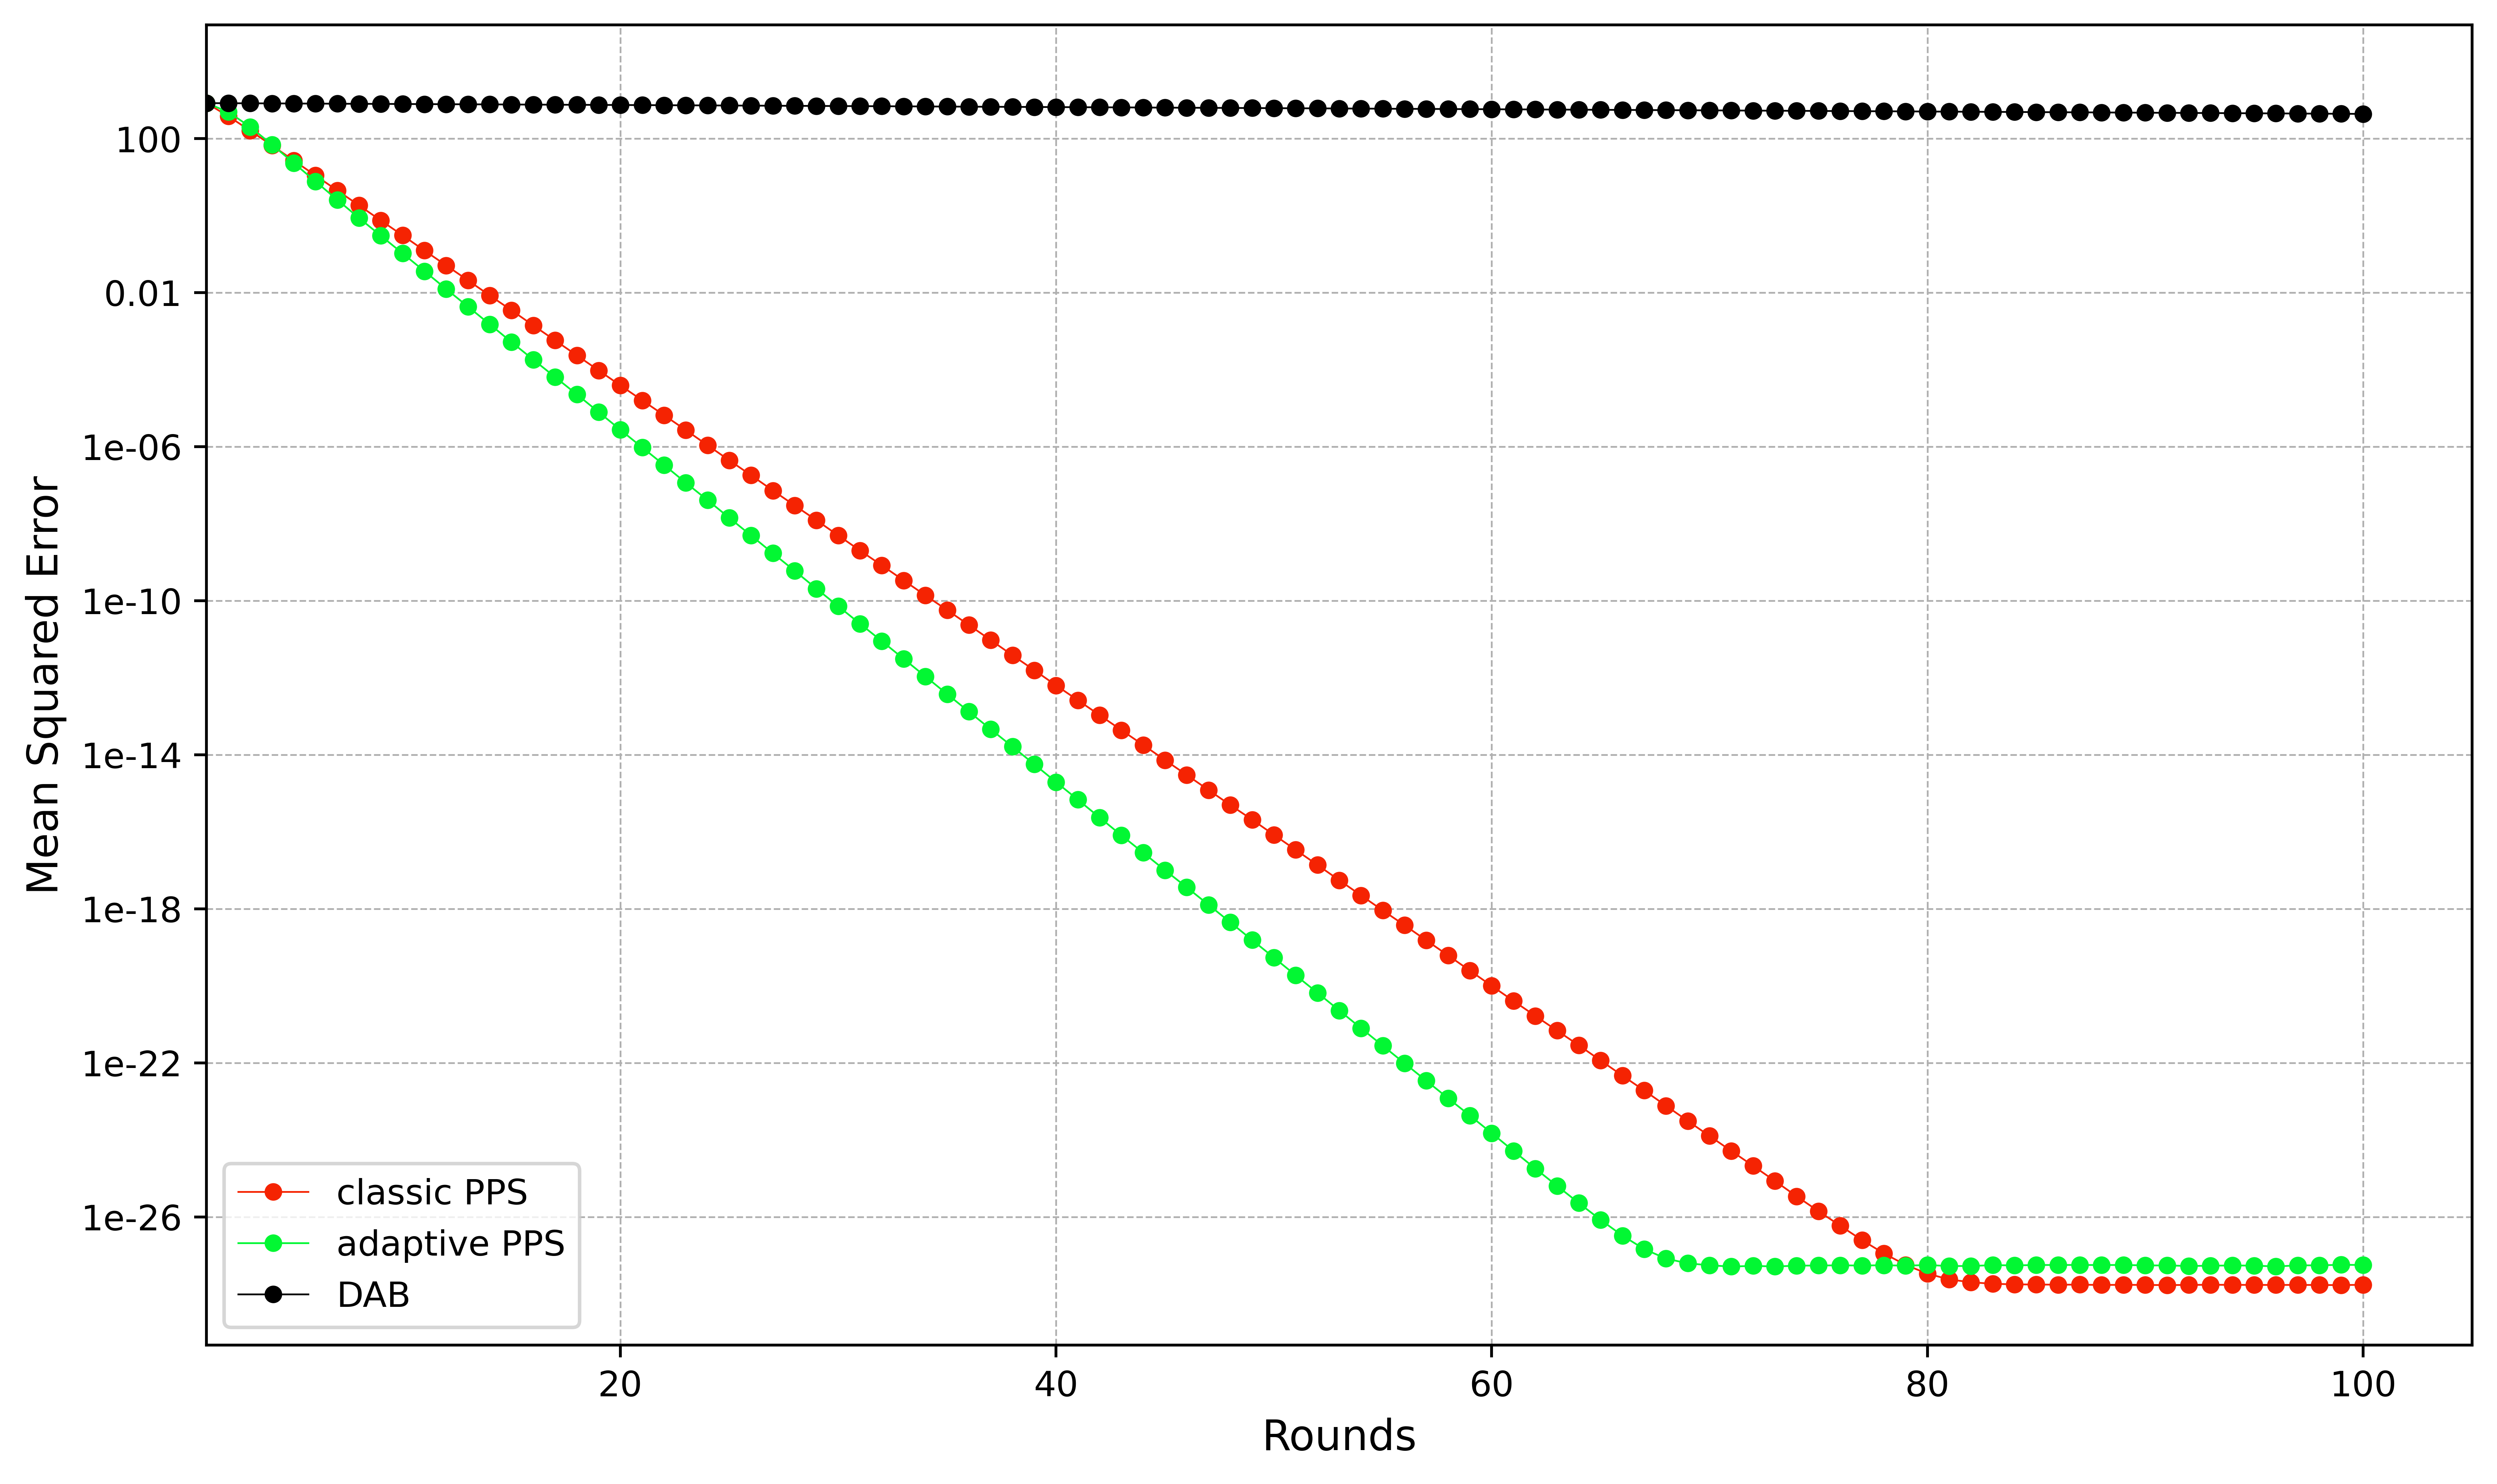
\includegraphics[width=0.49\linewidth]{figures/Simulation_outcomes/CompleteGraph/DAB_vs_PPS_CG_r100_n1024_averaged_log.png}}
    \hfil
        \subfloat[]{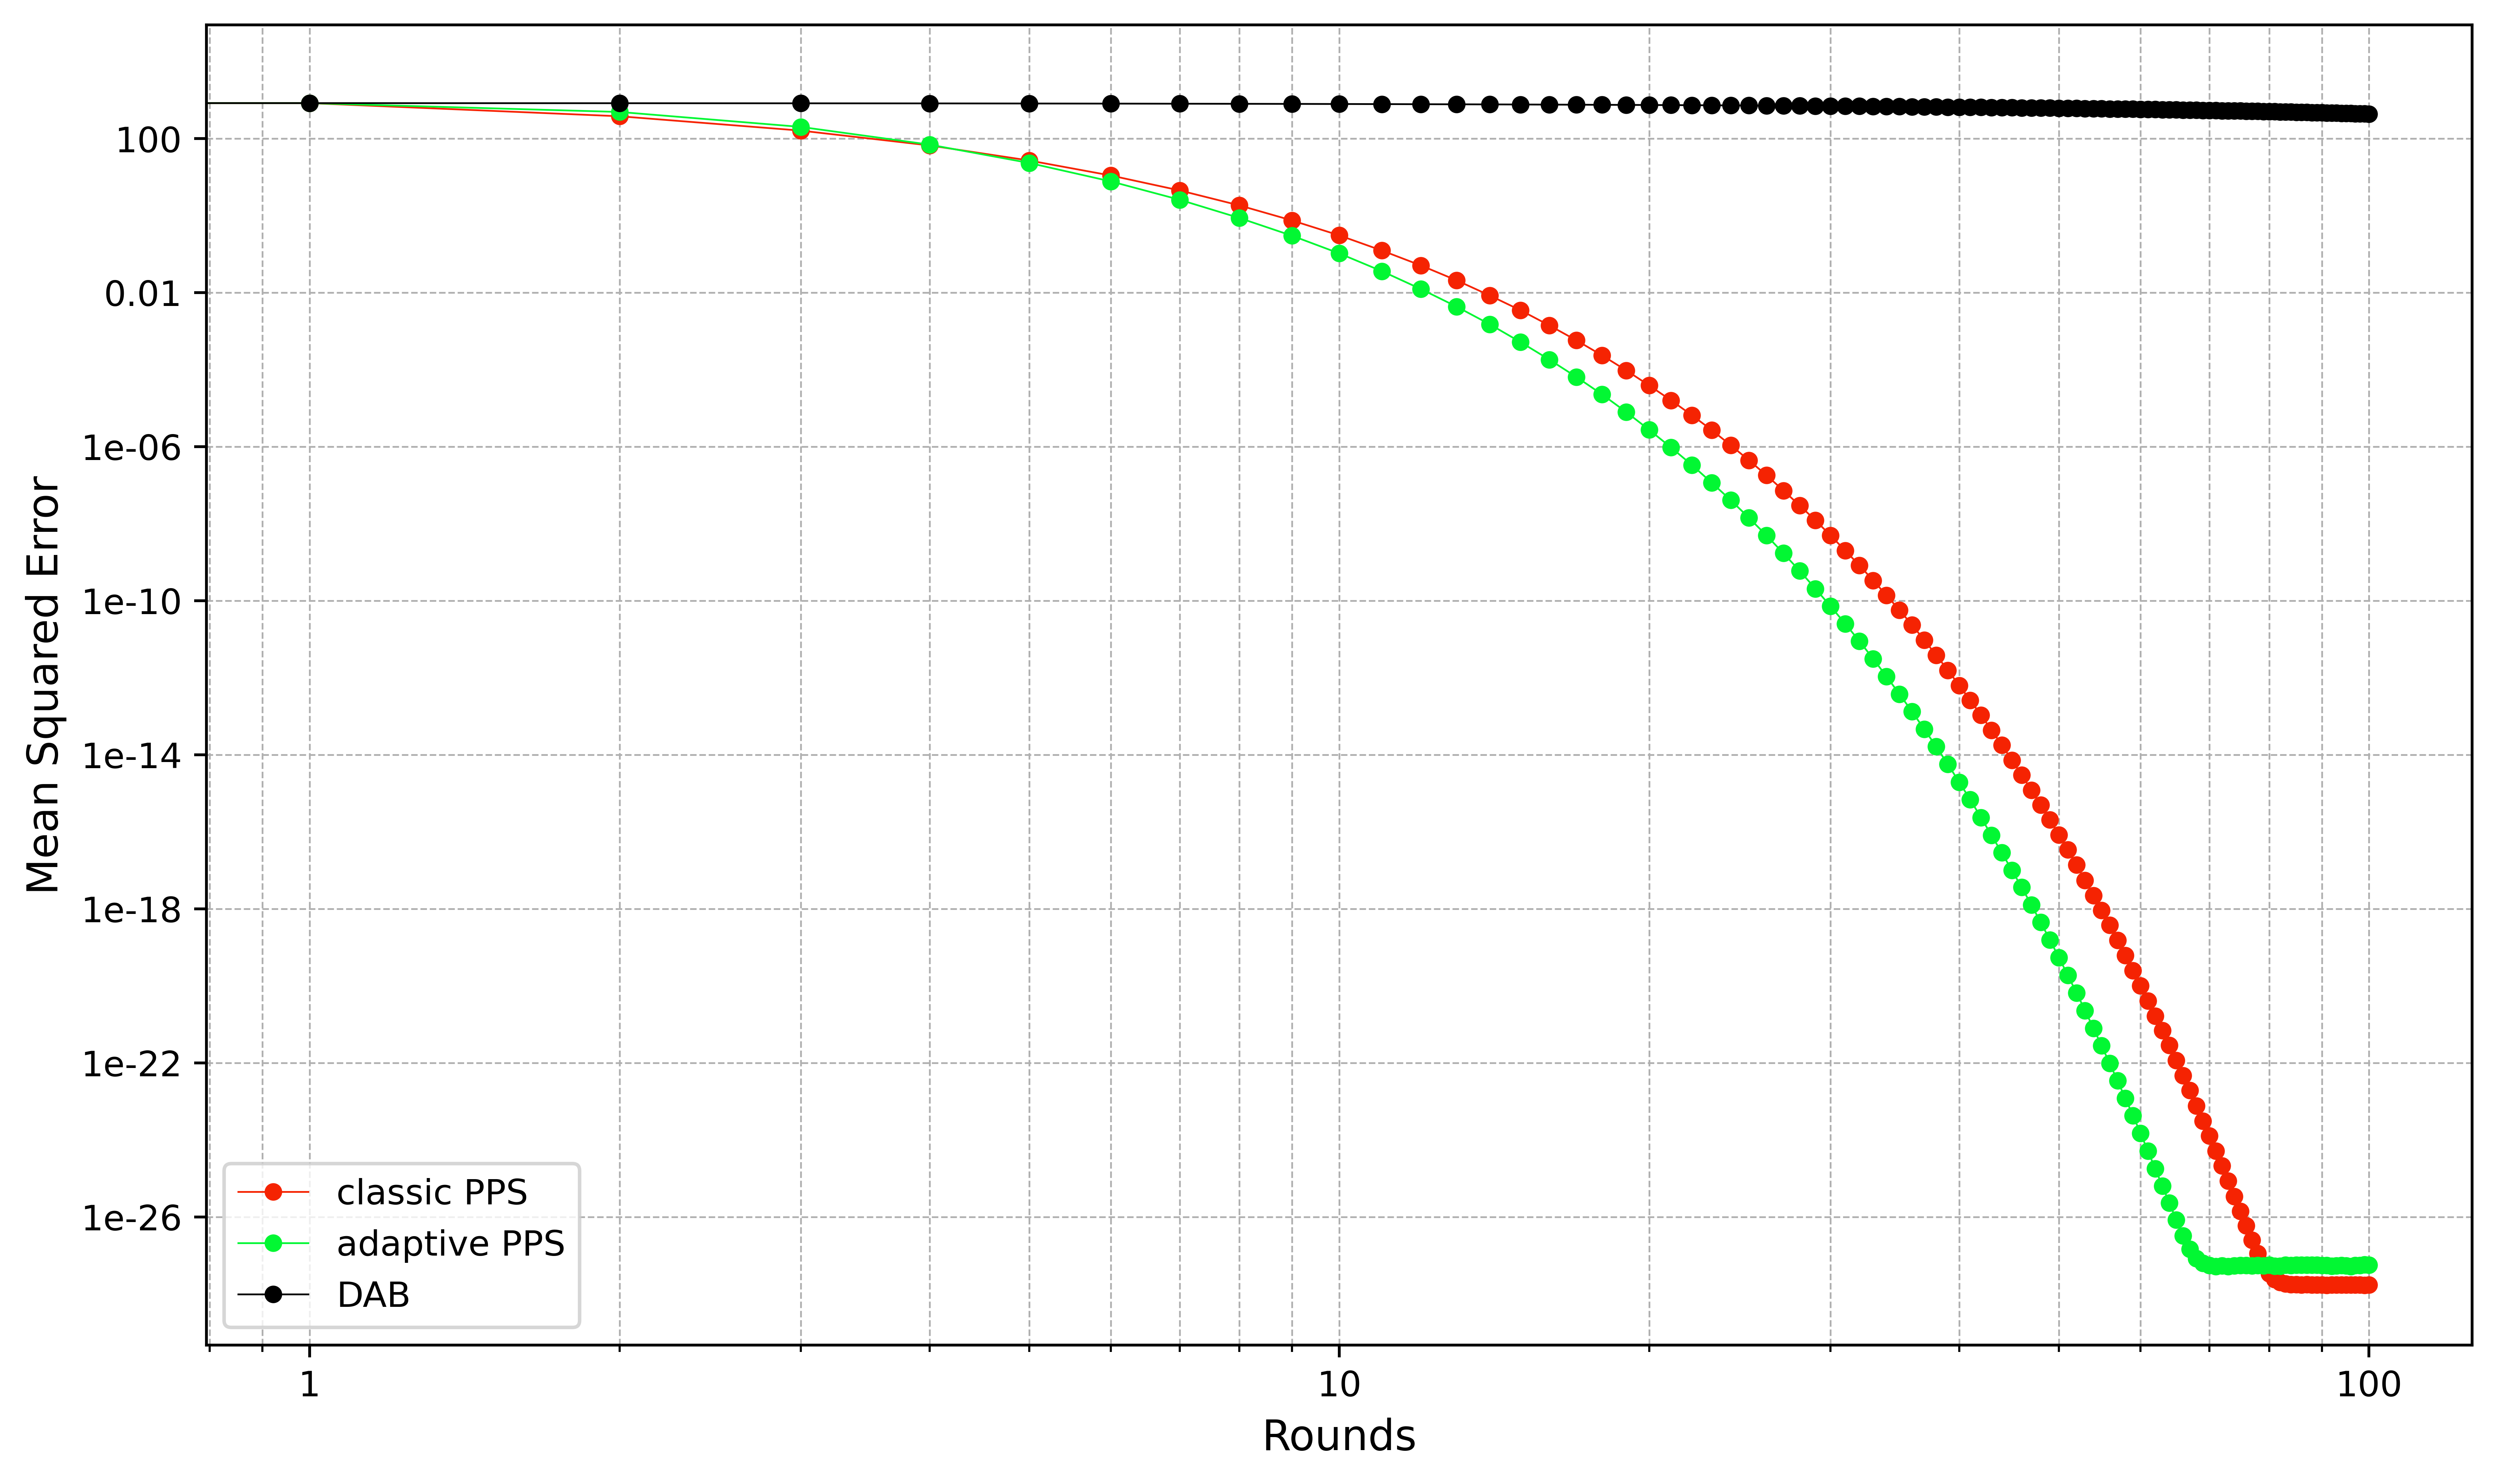
\includegraphics[width=0.49\linewidth]{figures/Simulation_outcomes/CompleteGraph/DAB_vs_PPS_CG_r100_n1024_averaged_loglog.png}}
    \caption{Complete graph - mean squared error per rounds - log-linear
    and log-log}
        \label{fig:completegraphMSEperRoundLogLog}
\end{figure}

Figure \ref{fig:completegraphMSEperRoundLogLog} a) presents the MSE reduction per round for the three load balancing algorithms simulated on the Complete graph $K_{1024}$ on a log-linear graph. Figure \ref{fig:completegraphMSEperRoundLogLog} b) shows the log-log graph of the same. The DAB curve (black curve) shows a linear trend and a gentle decrease of the MSE over the 100 rounds. The DAB performs poorly since it uses a fixed, deterministic load redistribution rule for its nodes, where each node selects the minimally loaded neighbor and proposes a load transfer. In a Complete graph where each node is interconnected, the same few nodes that hold the load of amount $L_{min}$ are the nodes that are receiving all the proposals. Since each minimal neighbor only accepts one proposal per round, the number of load transfers is heavily limited, resulting in slow MSE reduction. The PPS and ATPPS algorithms leverage the high connectivity of the network more effectively, due to their randomized nature. The PPS curve (red curve) exhibits a steady decrease in MSE, therefore showing efficient MSE reduction over time. Since all nodes are equally connected, no structural constraints slow down the process of pushing and pulling loads from neighbors. However, PPS does not distinguish between nodes that are highly imbalanced and those that are nearly balanced, leading to unnecessary load transfers in later rounds. The ATPPS (green curve) achieves even faster MSE reduction than PPS. As the system nears equilibrium, ATPPS reduces redundant exchanges. The stagnation at around $1.8\times 10^{-19}$ ($-2^{64}$) in the simulation is due to the limitations of Java's double precision, which cannot represent all integers exactly beyond a threshold. As a result, small increments become too insignificant to alter the MSE value, causing stagnation. In summary, DAB underperforms due to limitations on the amount of load transfers. PPS improves upon this but lacks adaptive control, while ATPPS optimally balances load while avoiding unnecessary exchanges, making it the most effective approach in this setting.

Figure \ref{fig:dabCompleteModelFit} a) shows the linear regression fit for the MSE data of the DAB. The data aligns well with the model, but the exponential regression fit suits better in this case. Figure \ref{fig:dabCompleteModelFit} b) shows the exponential regression fit for the MSE data when the DAB as a load balancing strategy is applied to the network. Even though the curve might not suggest an exponential decay, the MSE data fits with the exponential regression model following the equation:
\begin{align}
    MSE_r=844.63*e^{-0.01*r}.    
\end{align}
The decay rate of -0.01 suggests a very slow decrease in MSE. The fitted curve and model seem very suitable for the MSE data, since the fitted curve aligns with the MSE data. The MSE data of the PPS is fitted to the exponential regression model for rounds 10 to 80. Over time, randomized exchanges smooth out load imbalances, leading to an exponential decay in MSE, as seen in figure \ref{fig:ppsCompleteModelFit}. The best-fit follows the equation:
\begin{align}
    MSE_r=2530.41*e^{-0.9*r}.    
\end{align}
The decay rate of -0.9 suggests a steeper decline in error. In Figure \ref{fig:atppsCompleteModelFit}, the exponential regression fit is visualized for the MSE data of the ATPPS curve in the Complete graph for rounds 10 to 65. The fitted curve is expressed by the equation:
\begin{align}
    MSE_r=4309.94*e^{-1.06*r}.    
\end{align}
A steep error reduction is indicated by the decay rate of -1.06. As the PPS, the ATPPS reduces the error very effectively in an exponential manner. Rounds 66 to 100 show a plateauing of the MSE data, caused by precision problems of the double datatype in Java. The adaptive mechanism provides a faster decline in error indicated by the decay rate of -1.06 versus the one of the PPS of -0.9.

Figure \ref{fig:completegrapslopes} visualizes a heat map of the slopes in both the log-linear a) and log-log b) representations for the three load balancing algorithms across different regions of the graph. The values reflect how steeply the MSE decreases over rounds. In the start region (rounds 1 to 10), PPS and ATPPS achieve a decay rate of -0.38 and -0.43, while DAB only reaches a value of $-2.6 \times 10^{-3}$. In the early phase, PPS and ATPPS have a much faster exponential decay in MSE than DAB, meaning they reduce error more effectively at the start. In the middle region (rounds 11 to 65), the PPS and ATPPS algorithms slightly accelerate the error reduction to -0.39 for the PPS and -0.46 for the ATPPS. DAB proceeds to reduce the error in a slow manner. The decay rate is as low as $-2.7 \times 10^{-3}$ for the DAB. DAB has shallower negative slopes overall. The stagnation behavior described above can also be seen in the decay rate, which is close to zero in the final region, i.e. precisely when the ATPPS curve begins to stagnate. The PPS curve does not stagnate until round 80, so the decay rate is still relatively high. The general decay rates (rounds 1-100) for PPS and ATPPS (-0.3) are steeper than DAB ($-2.8 \times 10^{-3}$), which suggests that PPS and ATPPS converge much faster on average. The MSE is reduced significantly by the PPS and ATPPS. The initial MSE value of $832$ is reduced to $1.72 \times 10^{-28}$ for the PPS and $5.63 \times 10^{-28}$ for the ATPPS, while the DAB reduced the error to nearly half of the initial value, achieving a value of $436.84$.

\begin{figure}[!ht]
    \centering
        \subfloat[]{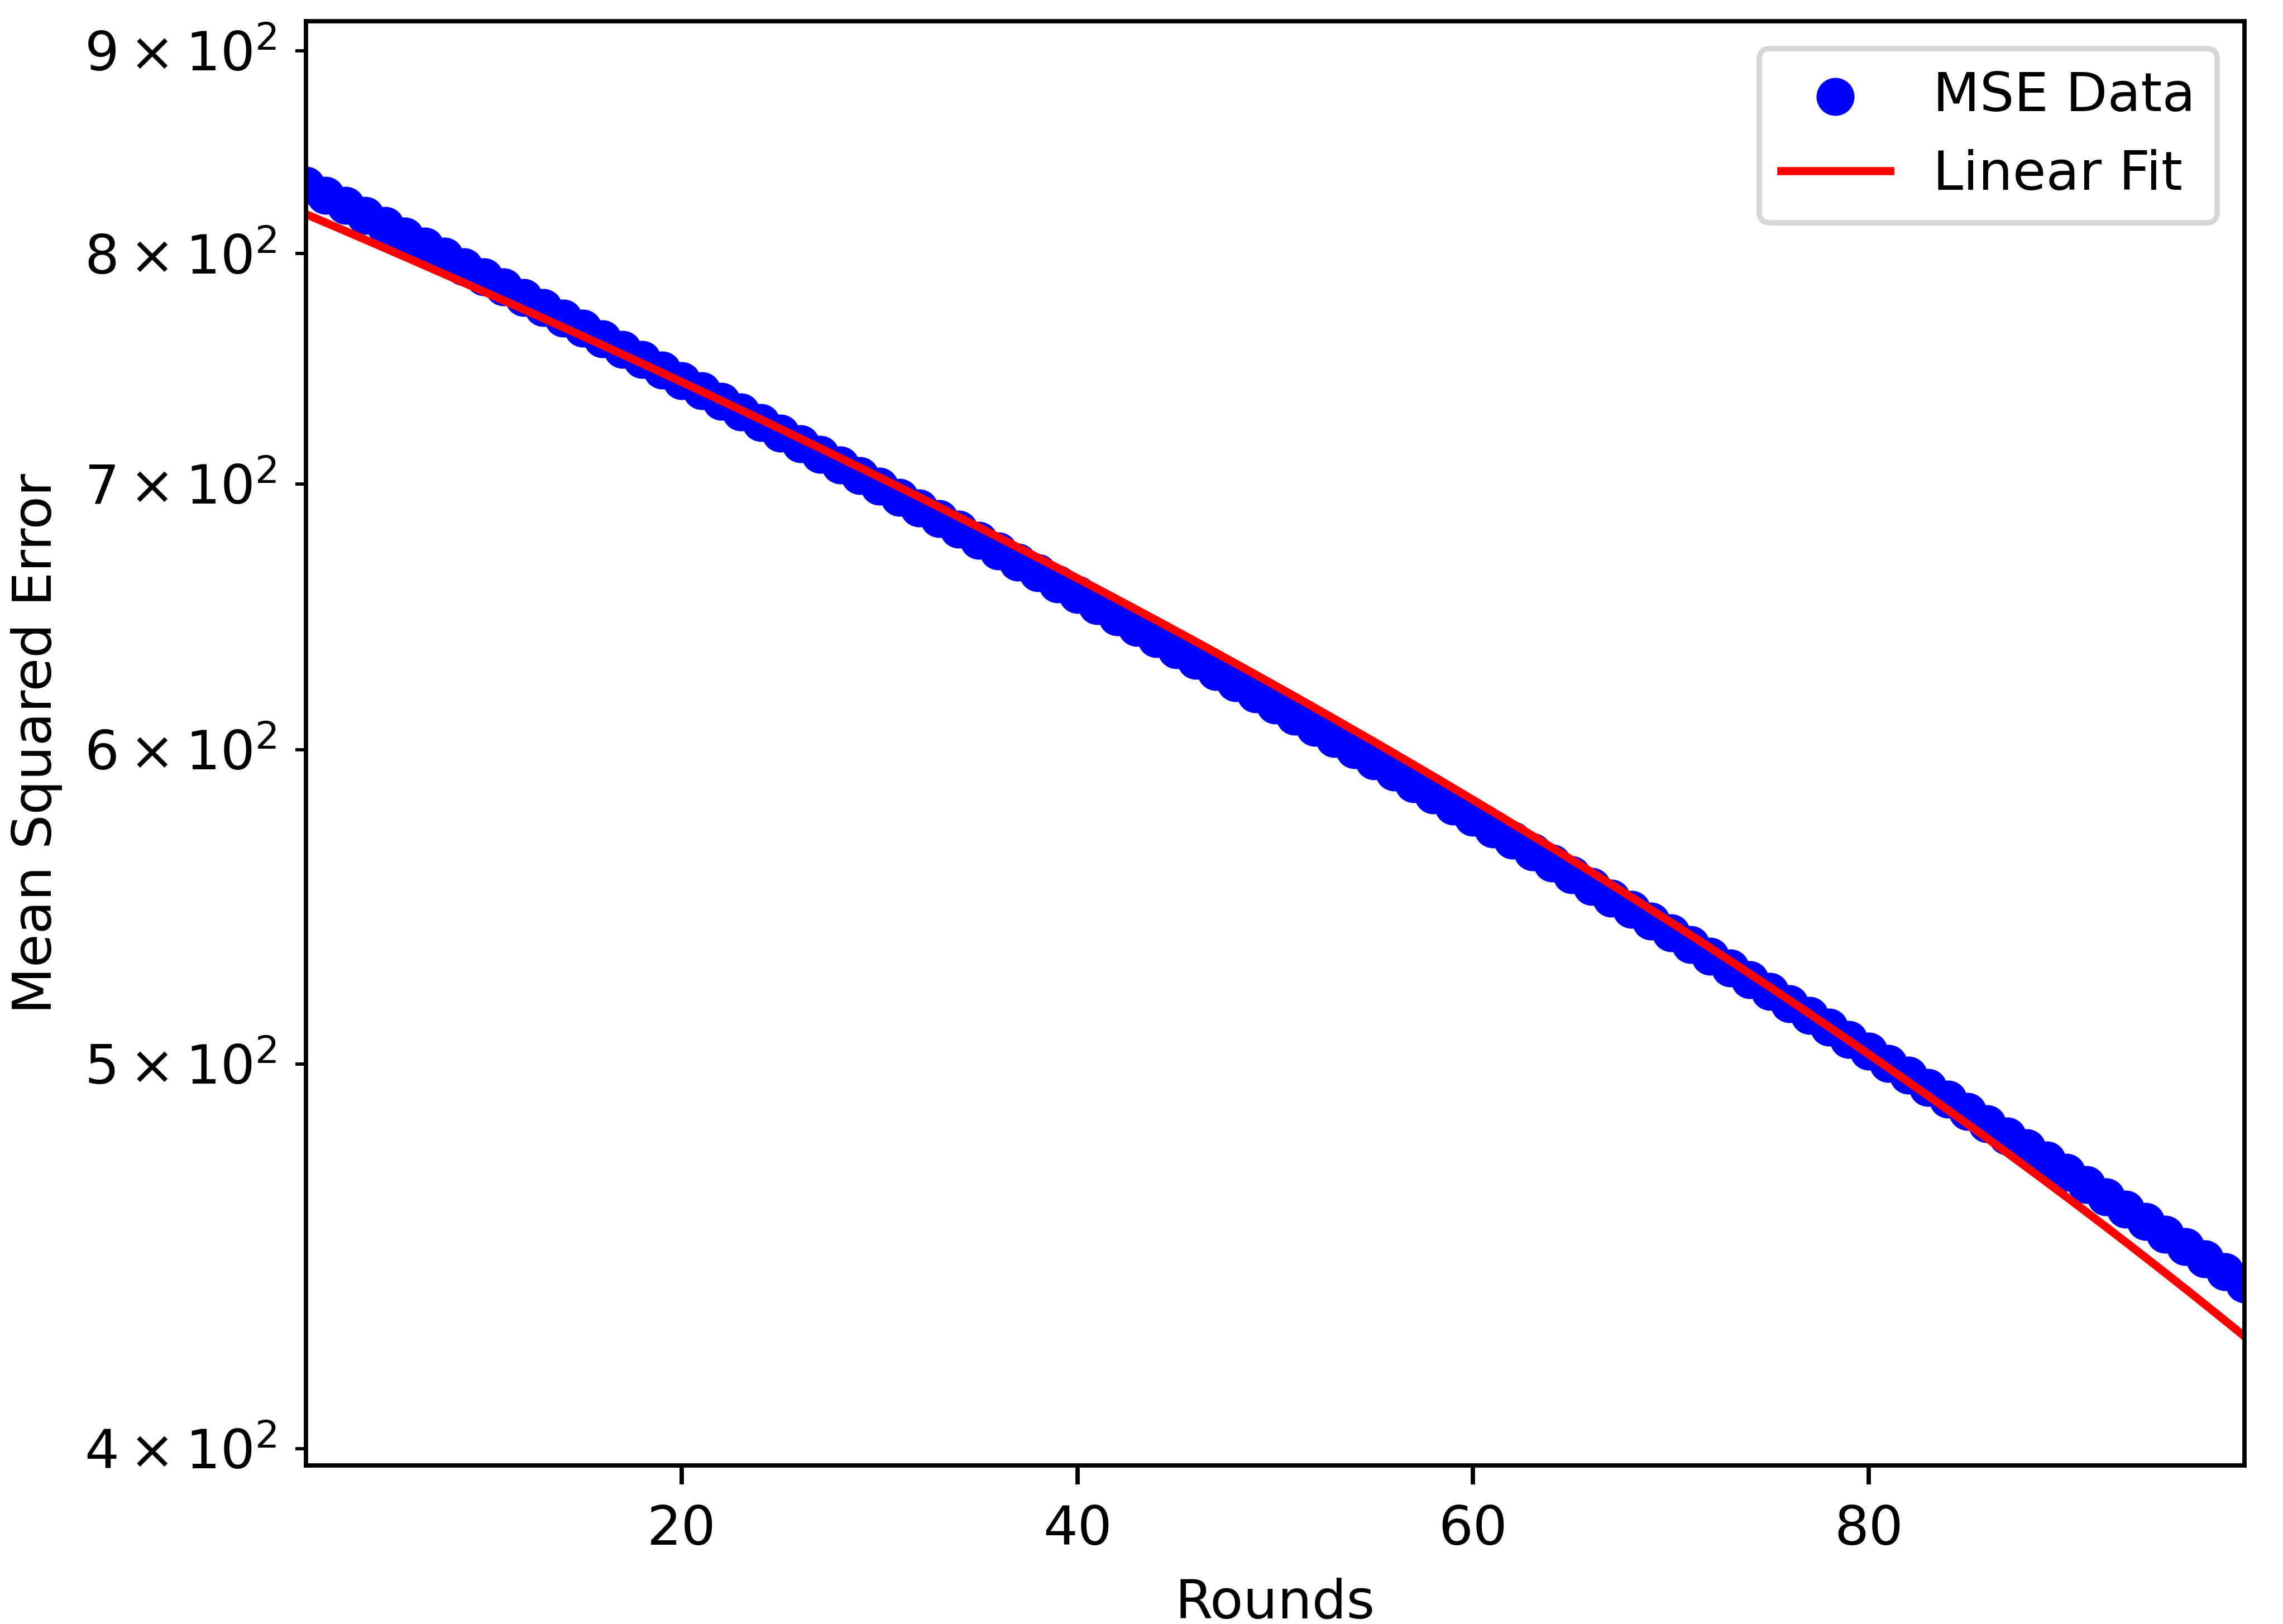
\includegraphics[width=0.49\linewidth]{figures/Simulation_outcomes/CompleteGraph/DAB/DAB_modelfitting_rounds_99_model_0.png}}
    \hfil
        \subfloat[]{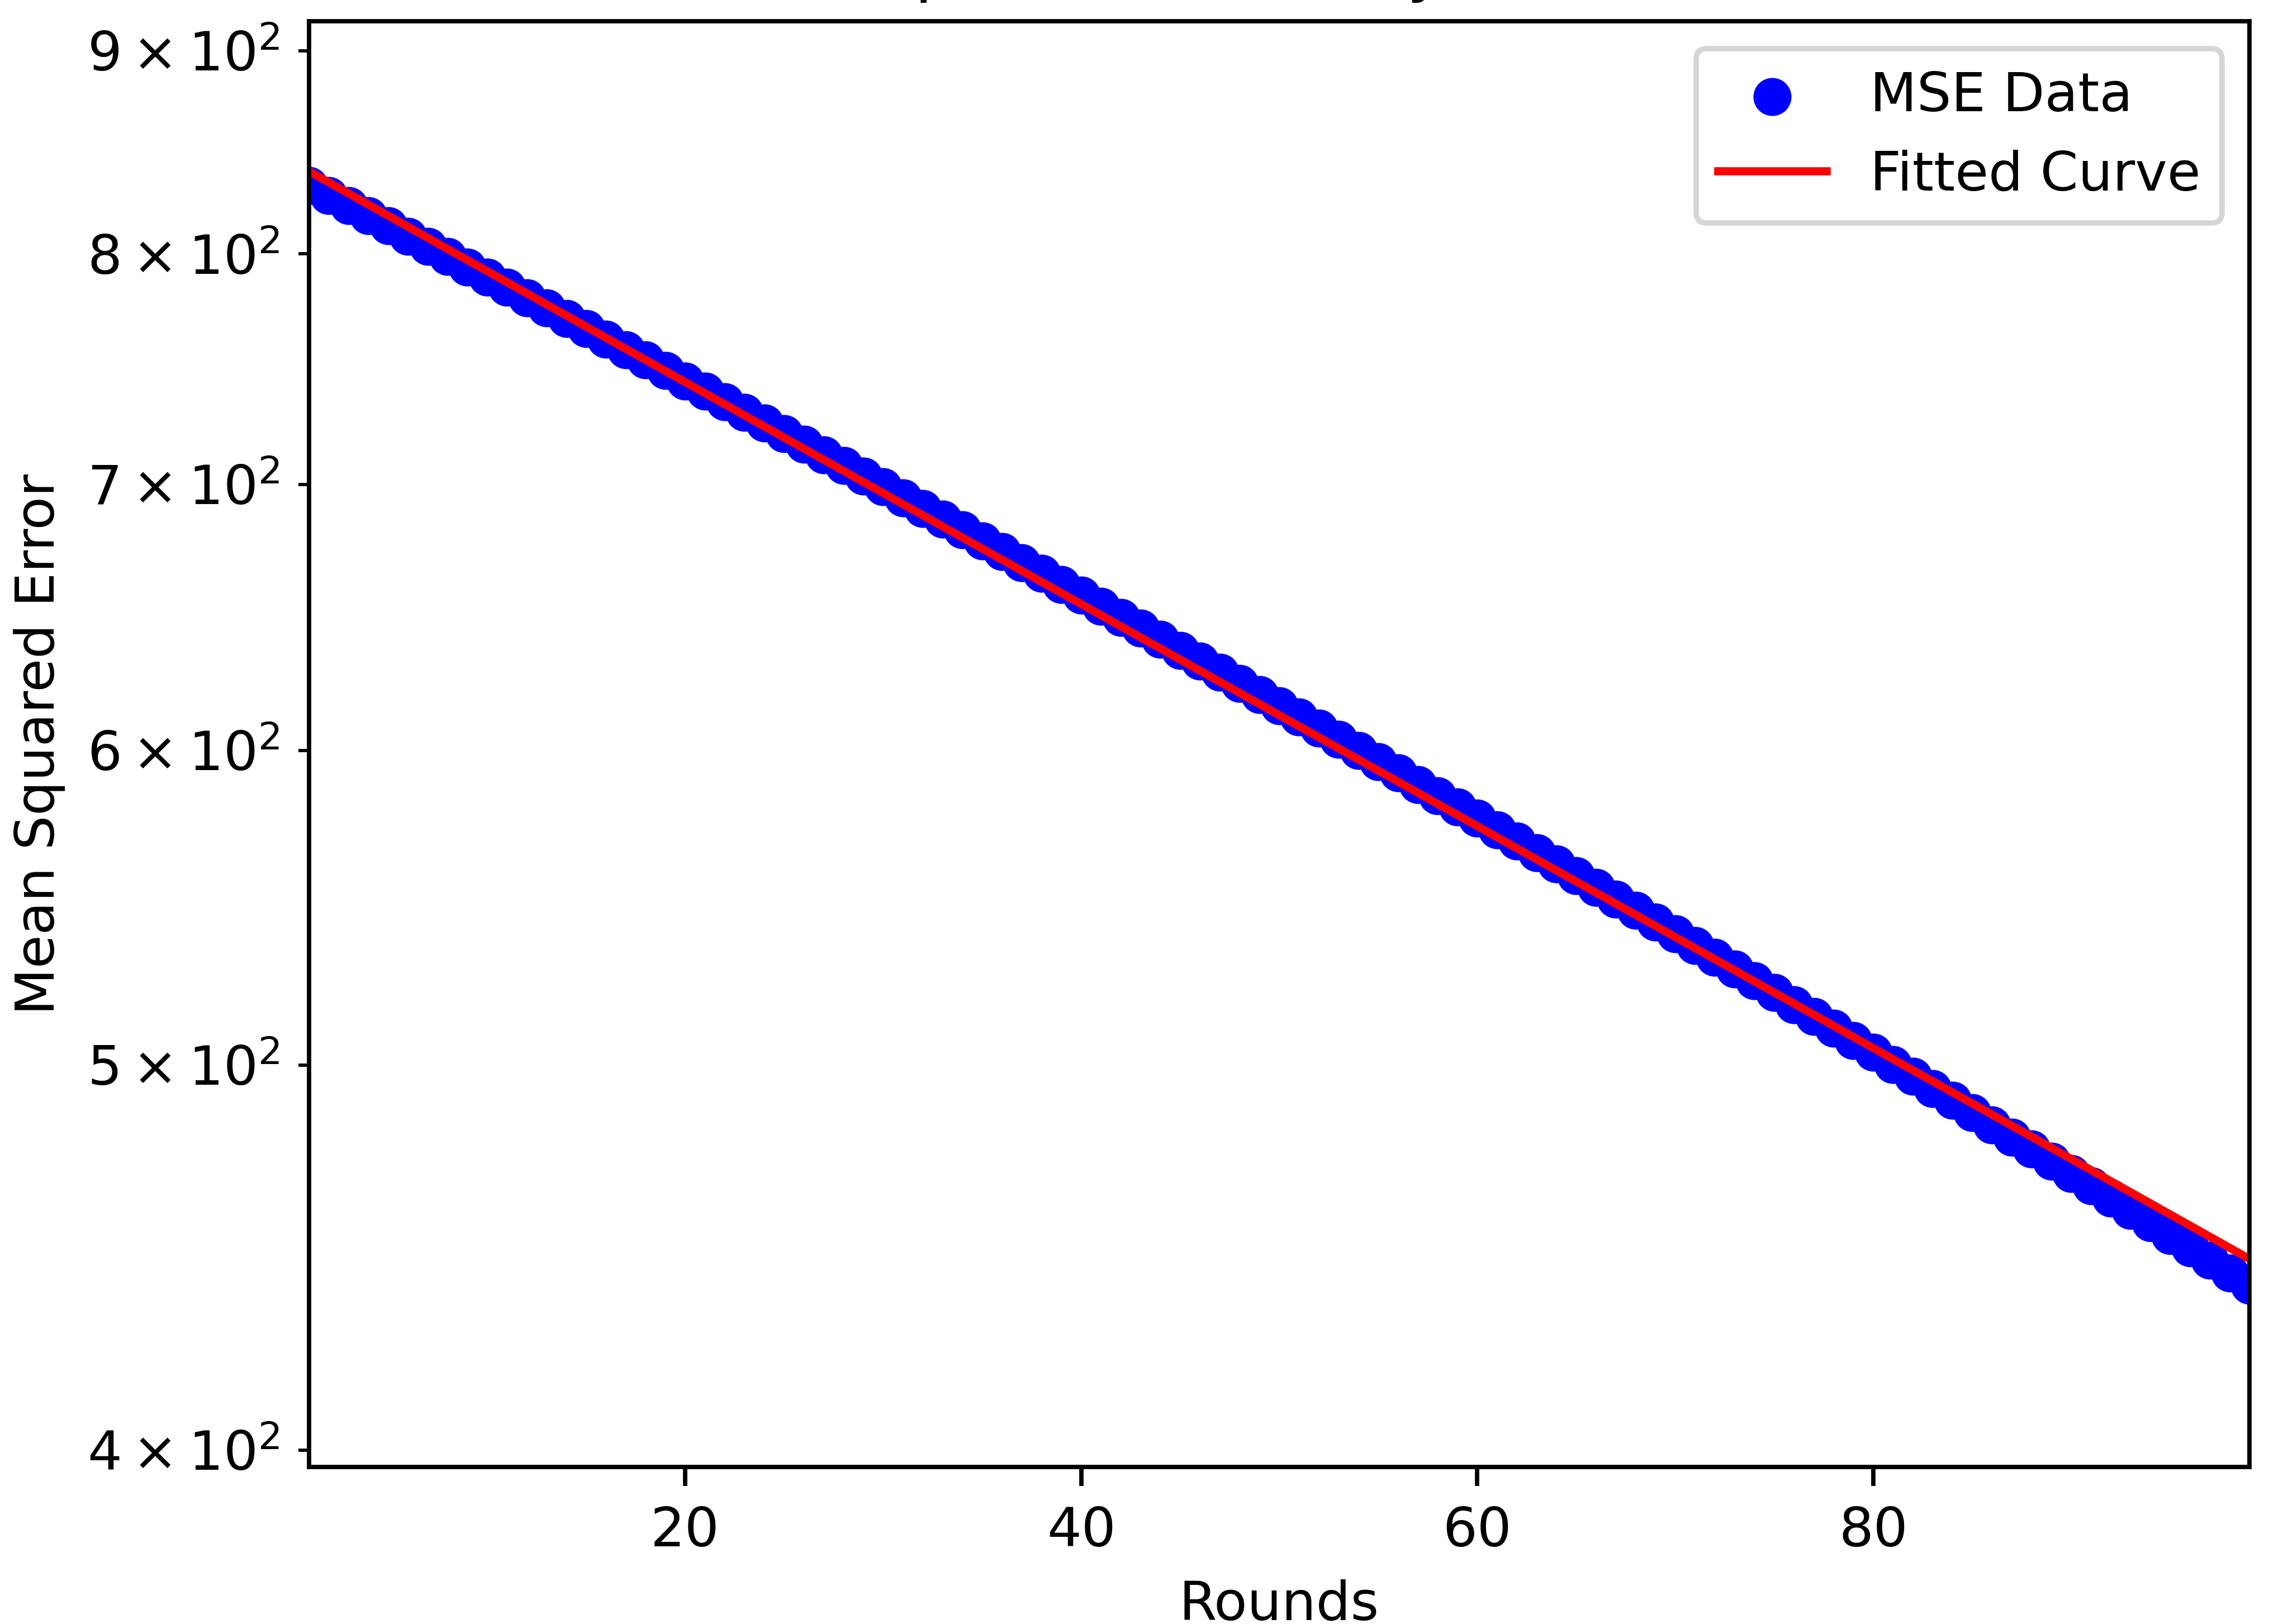
\includegraphics[width=0.49\linewidth]{figures/Simulation_outcomes/CompleteGraph/DAB/DAB_modelfitting_rounds_99_model_1.png}}
    \caption{Complete graph - linear and exponential regression - DAB}
        \label{fig:dabCompleteModelFit}
\end{figure}

\begin{figure}[]
    \centering
    \scalebox{0.8}{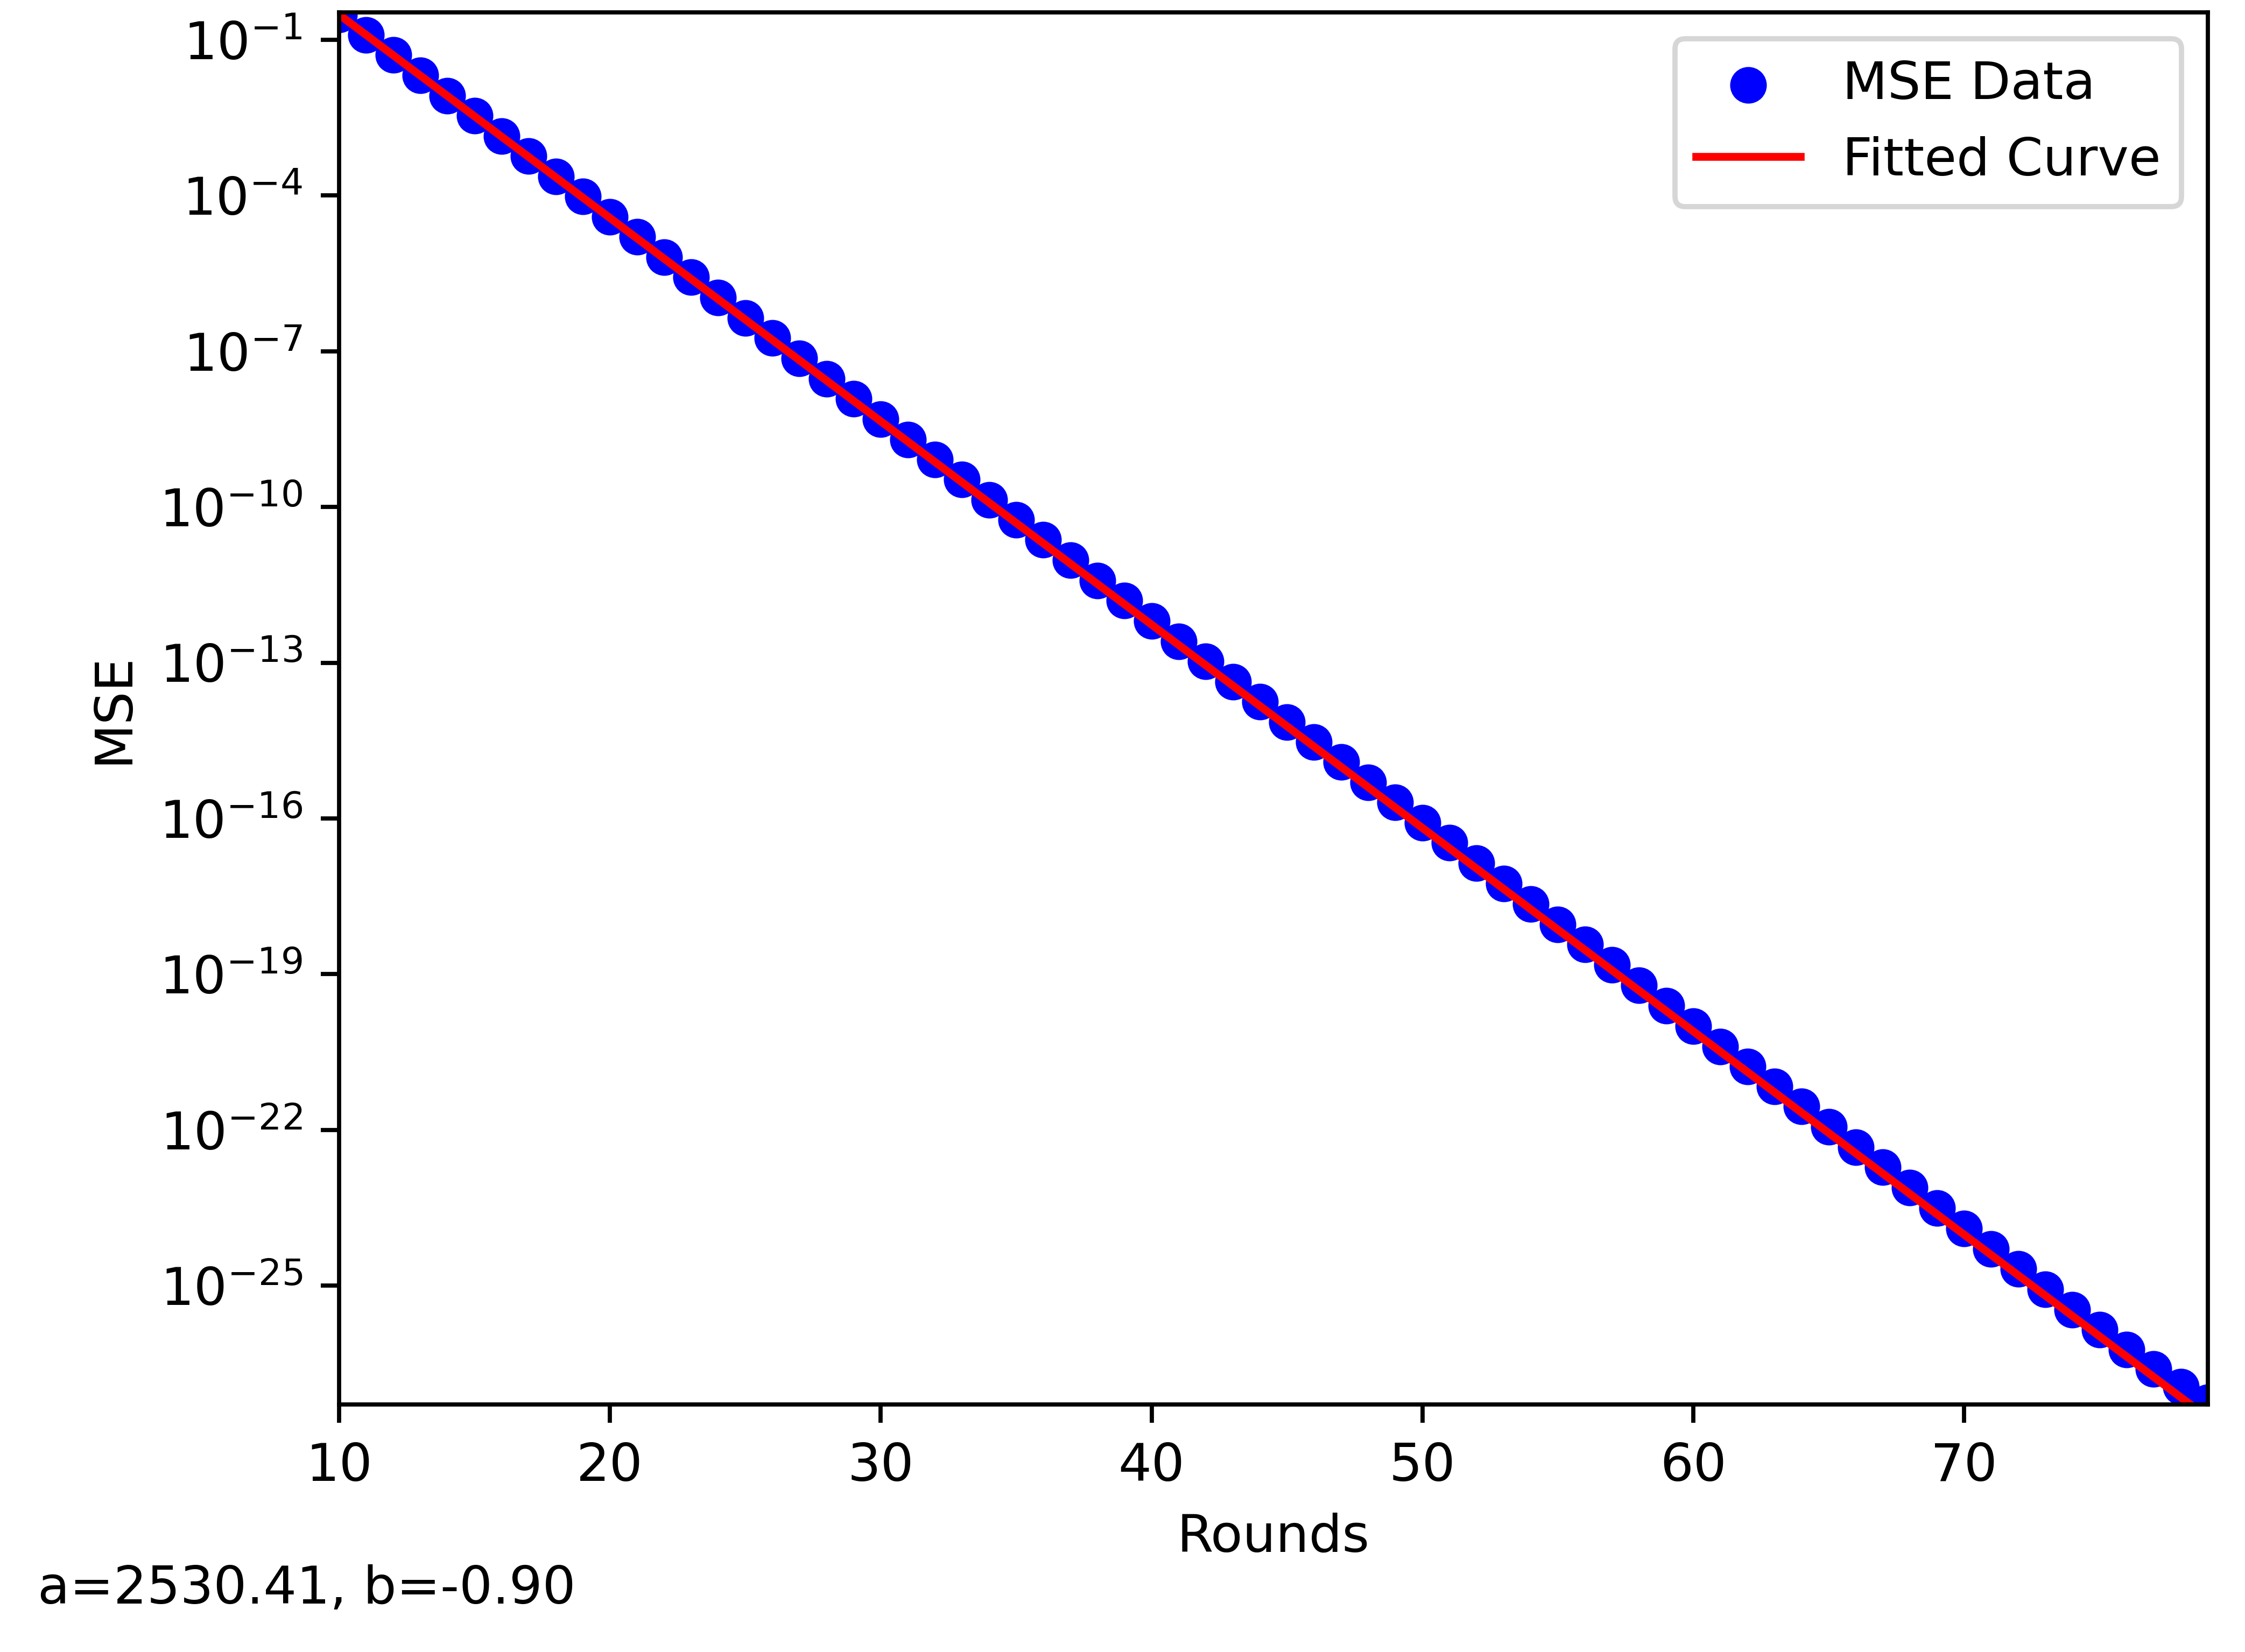
\includegraphics{figures/Simulation_outcomes/CompleteGraph/PPS/PPS_modelfitting_rounds_79_model_1.png}}
    \caption{Complete graph - exponential regression fit - PPS}
    \label{fig:ppsCompleteModelFit}
\end{figure}

\begin{figure}[]
    \centering
    \scalebox{0.8}{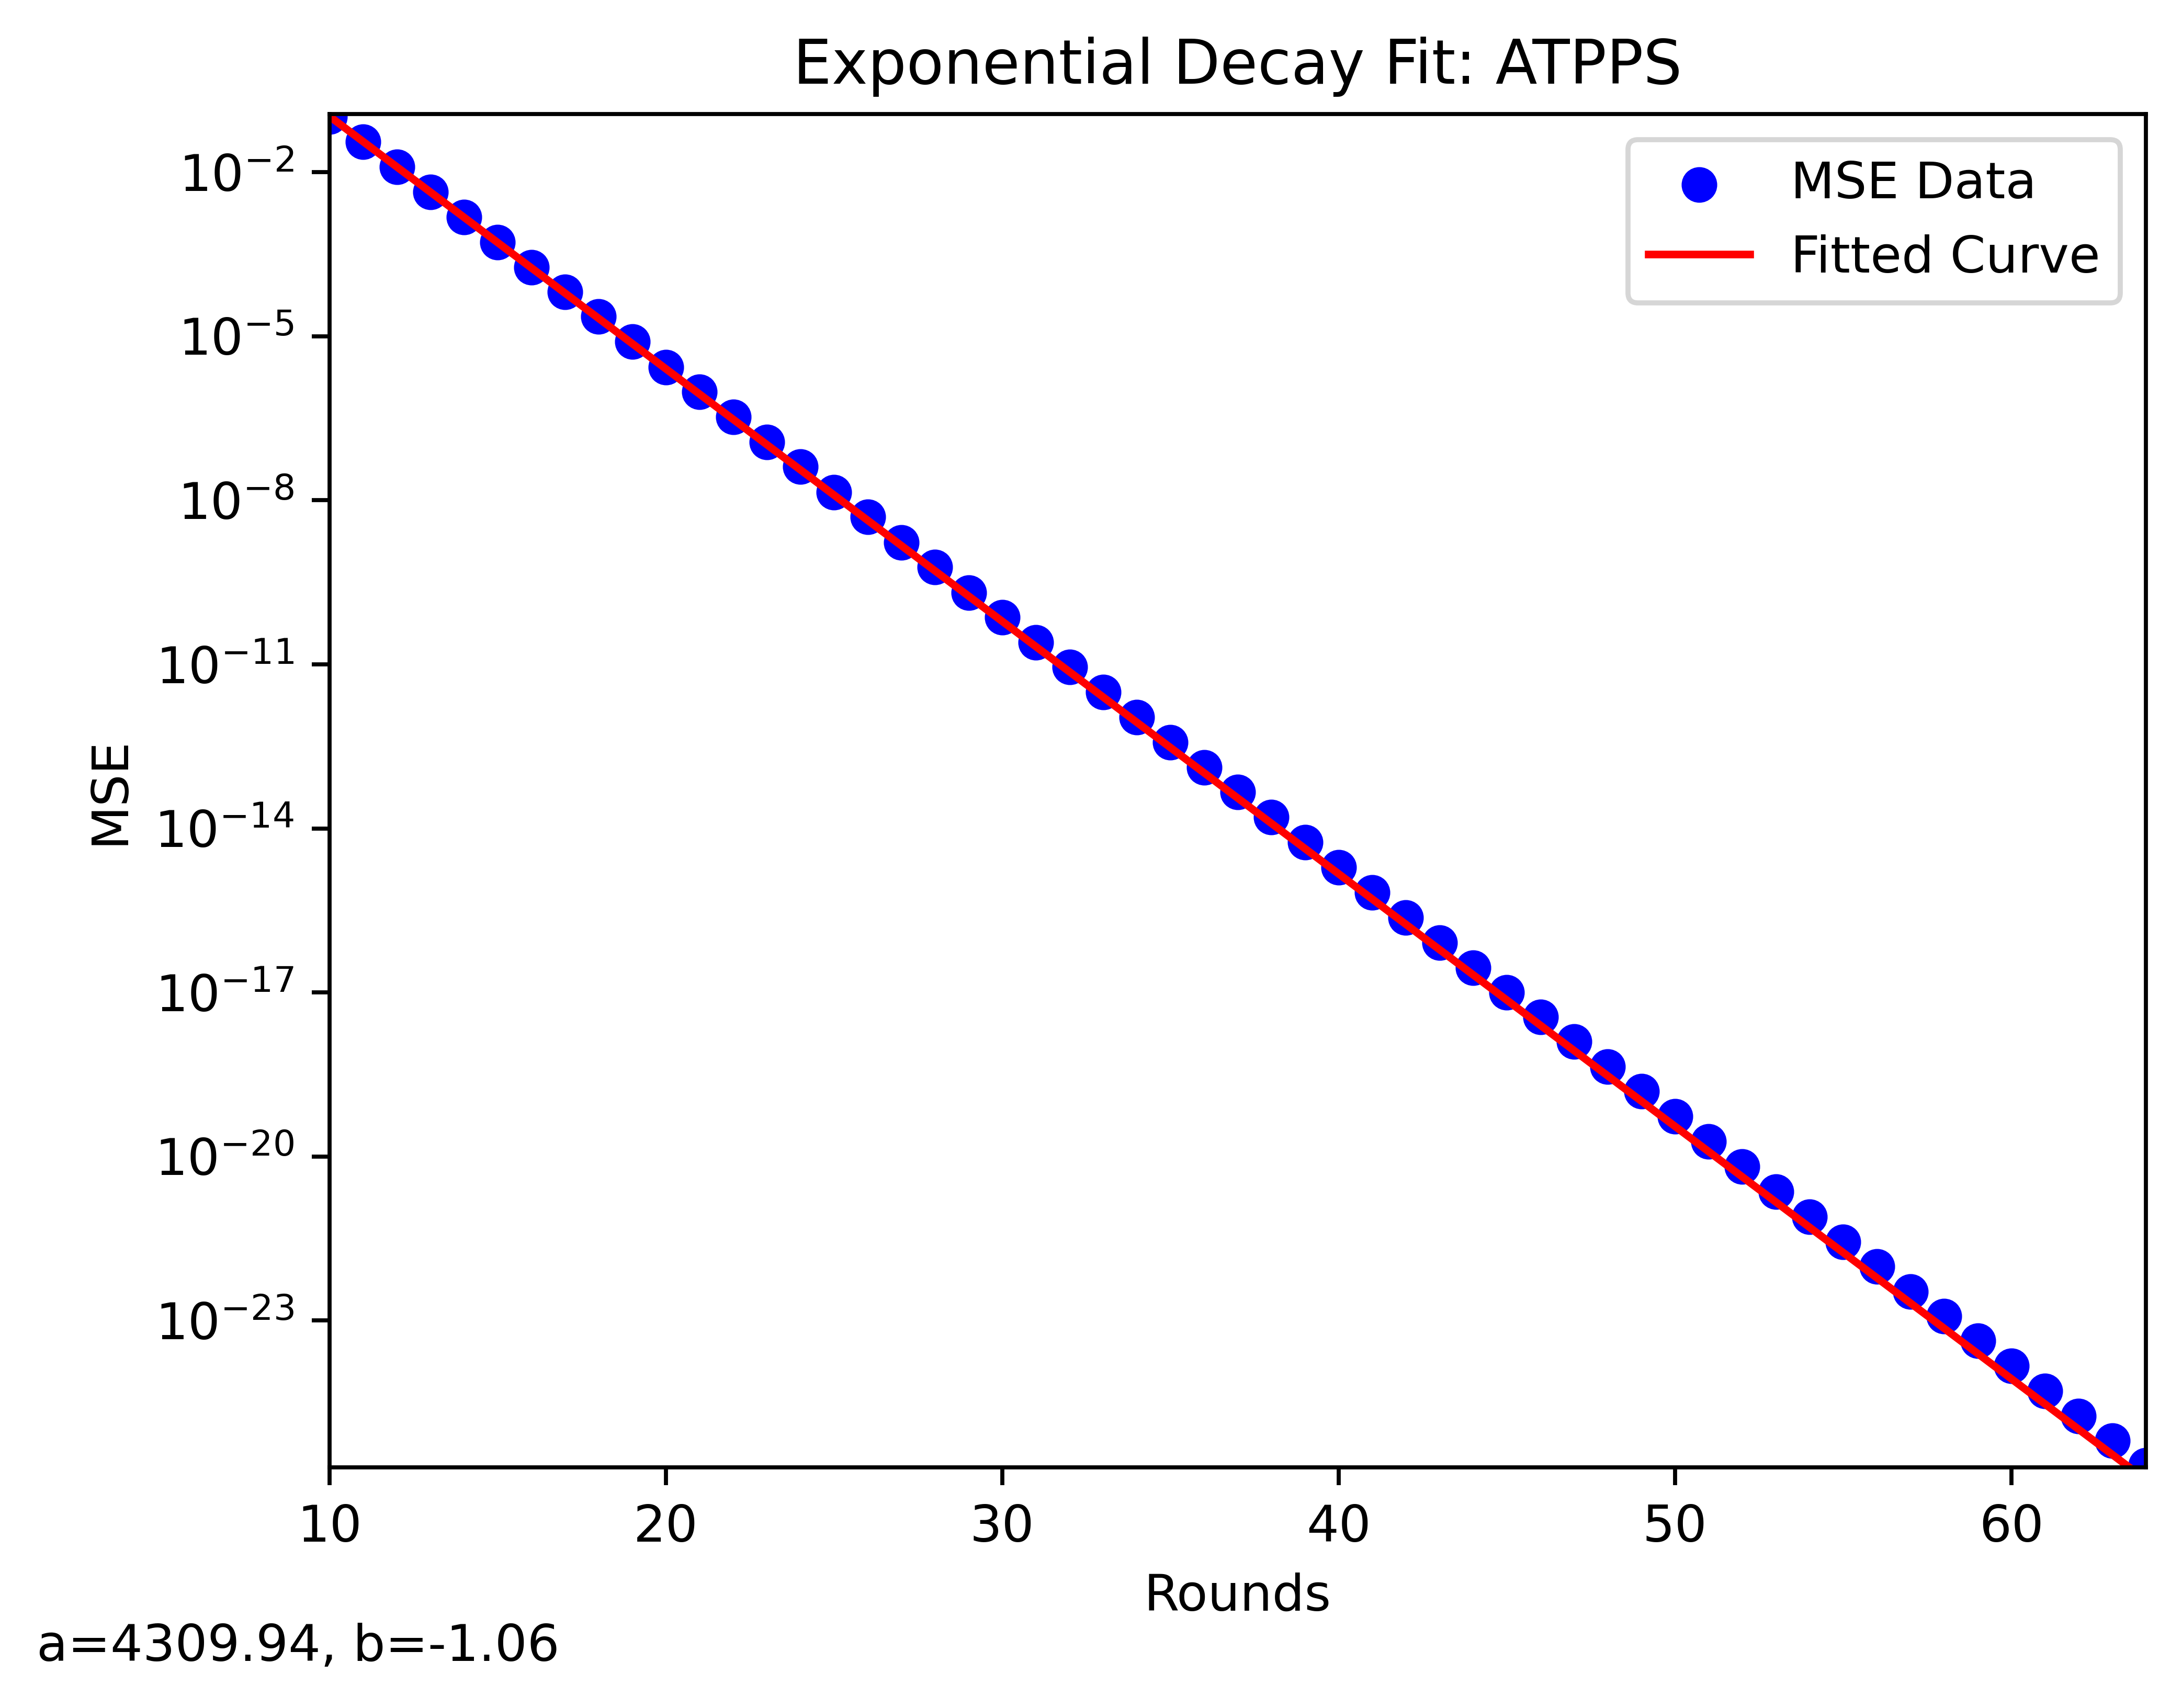
\includegraphics{figures/Simulation_outcomes/CompleteGraph/ATPPS/ATPPS_modelfitting_rounds_64_model_1.png}}
    \caption{Complete graph - exponential regression fit - ATPPS}
    \label{fig:atppsCompleteModelFit}
\end{figure}

\begin{figure}[!ht]
    \centering
        \subfloat[]{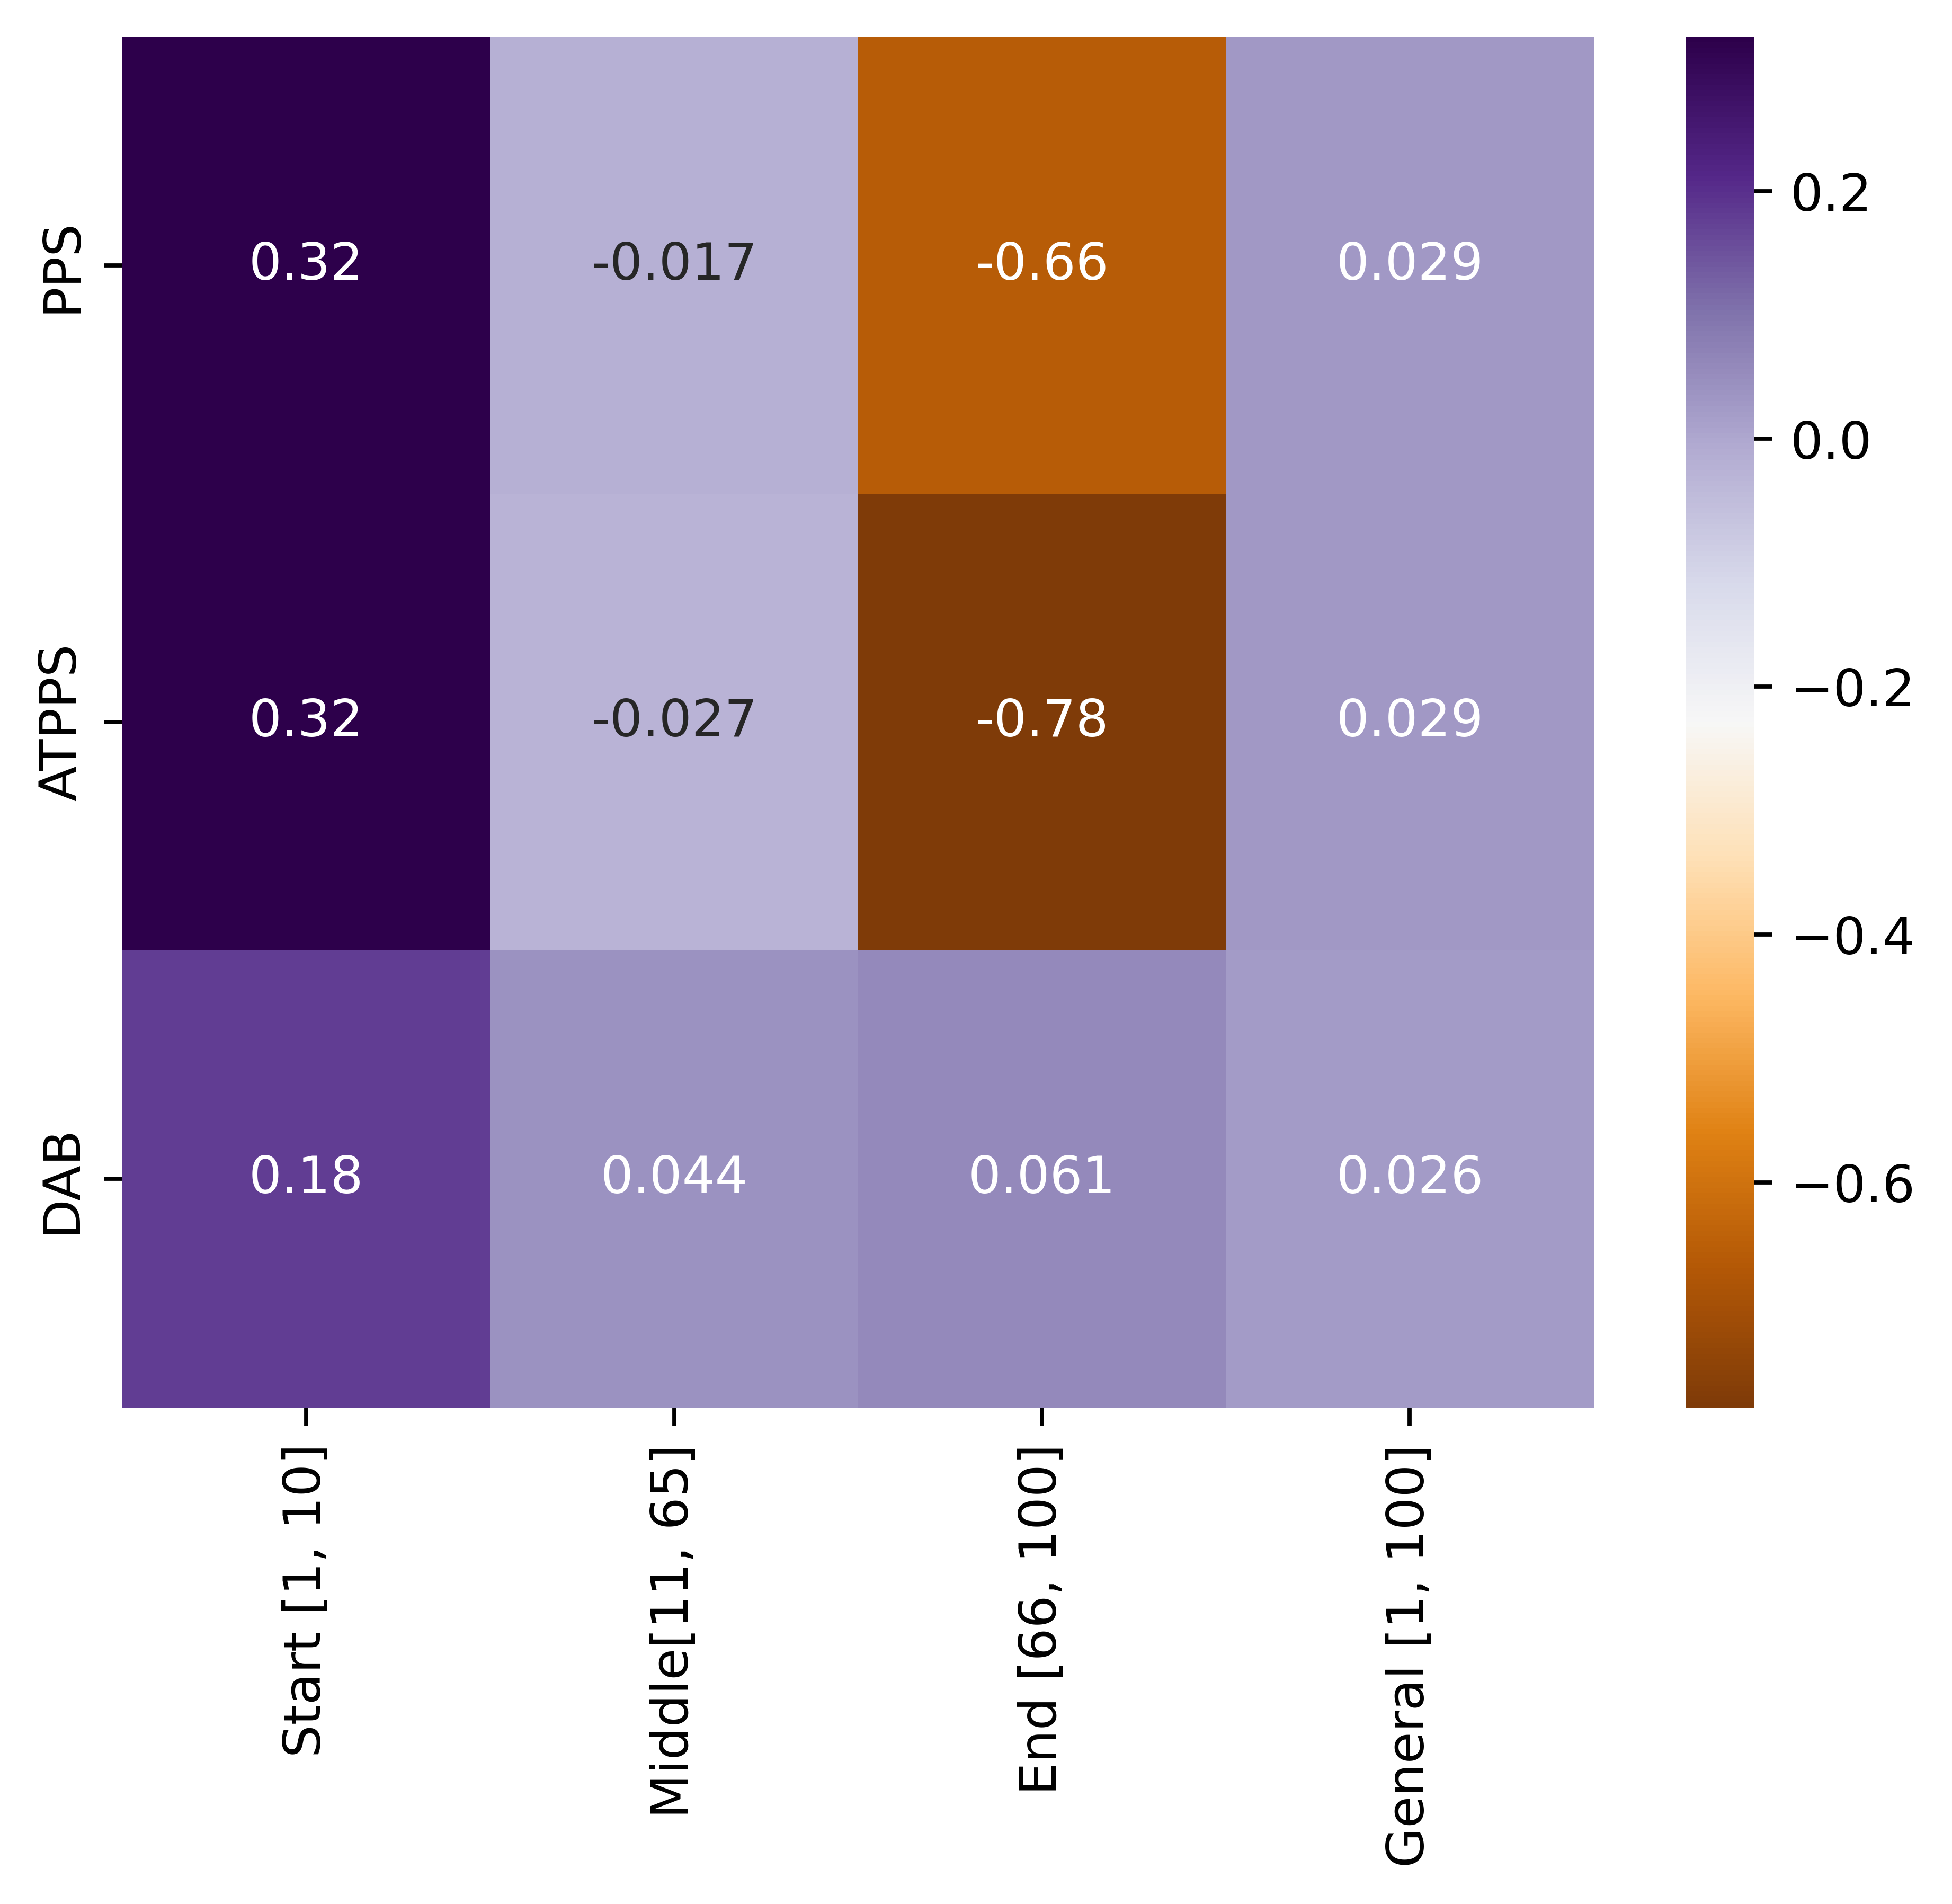
\includegraphics[width=0.49\linewidth]{figures/Simulation_outcomes/CompleteGraph/DAB_vs_PPS_vs_ATPPS_slopesheatmap_100rounds_log_lin.png}}
    \hfil
        \subfloat[]{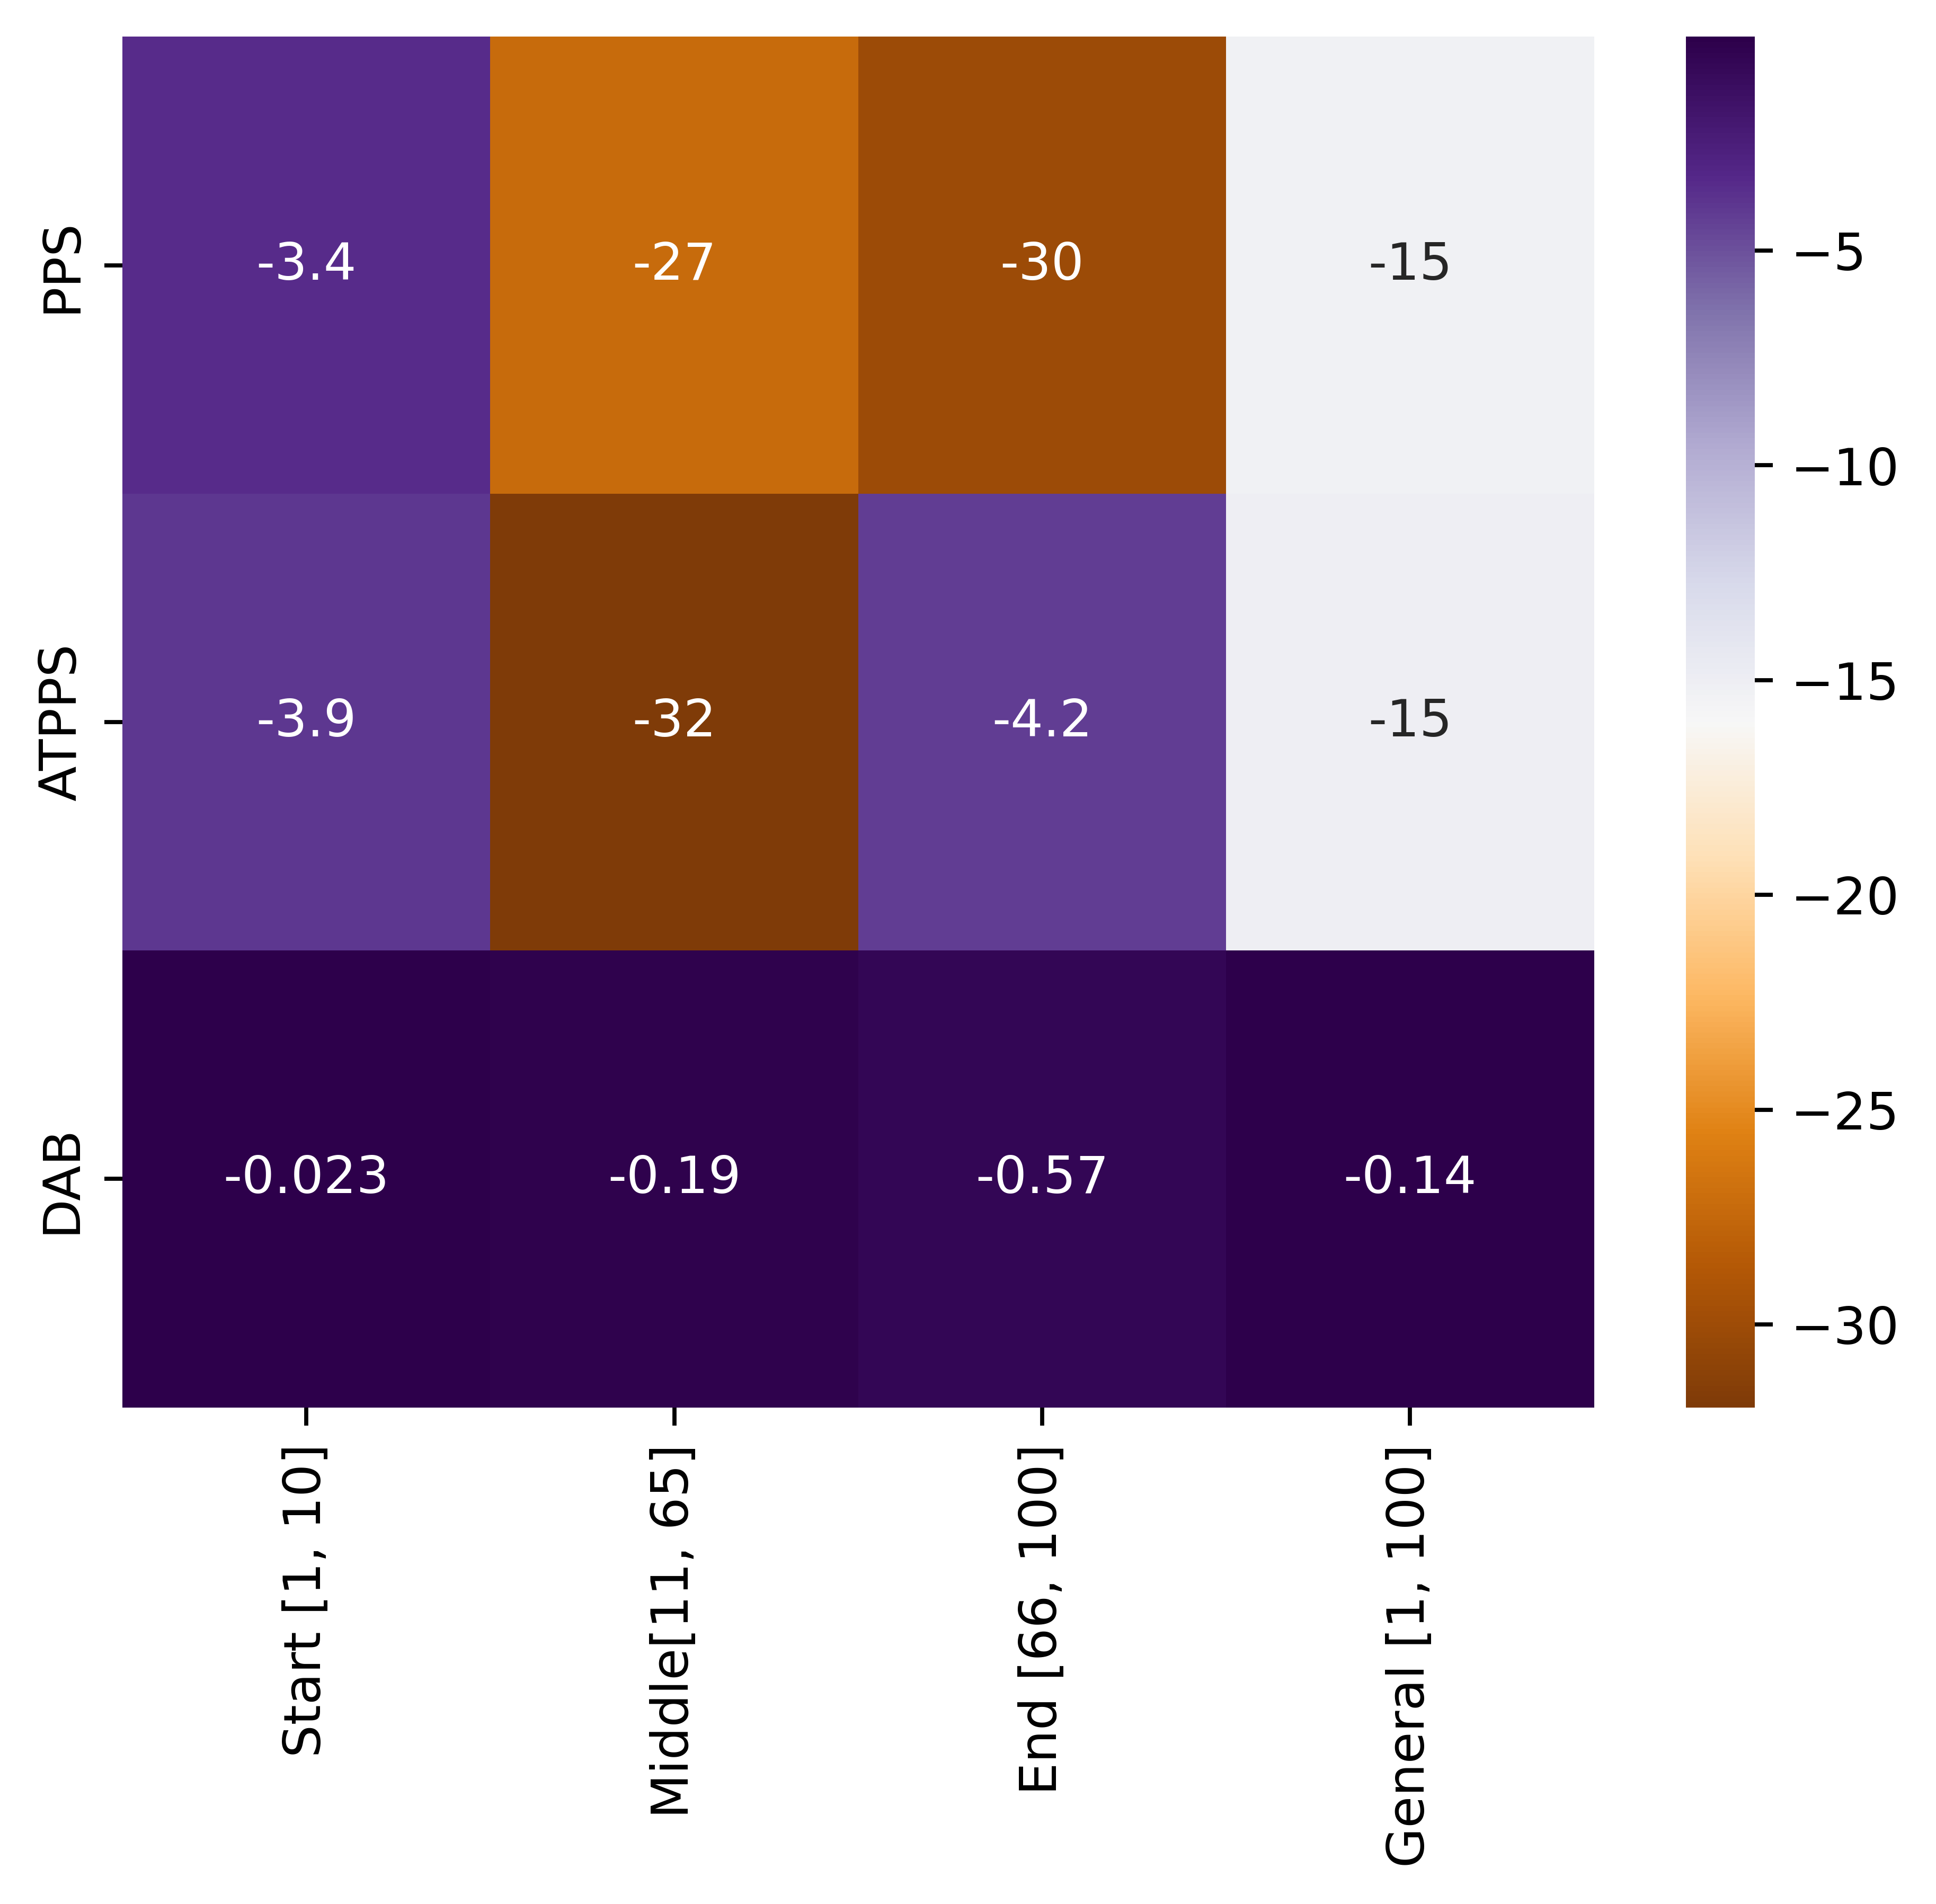
\includegraphics[width=0.49\linewidth]{figures/Simulation_outcomes/CompleteGraph/DAB_vs_PPS_vs_ATPPS_slopesheatmap_100rounds_log_log.png}}
    \caption{Complete graph - heat map of slopes per region - log-linear and log-log}
        \label{fig:completegrapslopes}
\end{figure}

\section{Star Graph}\label{sec:stargraph}
The behavior of the curves for the Star graph $S_{1024}$ simulations in figure \ref{fig:stargraphMSEperRoundLogLog} is similar to those for the Complete graph, with the difference that the PPS curve falls more steeply than the ATPPS curve. Figure \ref{fig:stargraphMSEperRoundLogLog} a) shows the log-linear representation of the MSE data, while figure \ref{fig:stargraphMSEperRoundLogLog} b) shows the log-log representation. Again, DAB shows a much slower MSE reduction compared to PPS and ATPPS, as indicated by the flatter slope of its curve. It converges minimally, with MSE reducing in a slow manner over rounds. This indicates that DAB is less efficient in balancing load in a Star graph, likely due to its deterministic nature and lack of dynamic adaptability. In the Star graph, all the leaves have the central node as a neighbor, meaning each leaf node selects the same central node to propose load transfers. When the central node has a higher load than the leaf requesting a transfer, no load transfer occurs between these two nodes, creating a bottleneck. Both PPS and ATPPS exhibit steep MSE reductions early on, as seen in the sharp downward trends in the log-log plot. The PPS balances load more efficiently than the ATPPS since it reduces MSE faster and reaches lower MSE values sooner (as of round 45). Again, the PPS and ATPPS curves start to plateau, as a result of the precision of double. The Push-Pull Sum-based algorithms draw an advantage from the Star graph, as the redistribution happens through the central node, which is chosen by every leaf node as a push destination. Following that, the central node redistributes parts of the load to the leaf nodes in magnitude of $\left(\frac{\frac{s_i,r}{2}}{N-1}, \frac{\frac{w_i,r}{2}}{N-1}\right)$.

As seen in figure \ref{fig:dabStarModelFit} b) the MSE data for the DAB-balanced network aligns nearly perfectly with the fitted curve of the exponential regression model given by the equation:
\begin{align}
    MSE_r=840.42*e^{-0.01*r}    
\end{align}
for the rounds 1 to 100. The decay rate of -0.01 indicates a very slow reduction in error. Since a linear decrease is suspected, the MSE data is also fitted to the linear regression model as presented in \ref{fig:dabStarModelFit} a). However, the exponential regression model aligns better with the DAB MSE data. From round to round, the improvement in the network remains minimal. This highlights the inability of the DAB to balance the network within 100 rounds to a satisfactory level. Figures \ref{fig:ppsStarModelFit} and \ref{fig:atppsStarModelFit} show the fitted curves for the MSE data of the PPS and ATPPS algorithms, respectively. The best-fit model for the MSE data of the PPS load balancing algorithm between rounds 10 to 45 follows the equation:
\begin{align}
    MSE_r=29794.60*e^{-1.39*r}.    
\end{align}
The rounds 10 to 45 exhibit the steepest decline in MSE, and for that reason, they have been fitted to an exponential regression model. The decay rate of $-1.39$ indicates a rapid reduction in error, especially in comparison to DAB. For the ATPPS, the MSE data fits best with the exponential model in the range of rounds 18 to 60, following the equation:
\begin{align}
    MSE_r=9329.40*e^{-1.05*r}.    
\end{align}
In Star graphs, the central node dominates communication, and load balancing heavily depends on that node. Threshold-based adjustments do not significantly impact performance under these conditions. The discrepancy between the two Push-Pull Sum-based algorithms can be explained by the fact that the ATPPS limits the number of messages due to the conditional threshold-based load transfer, which means that there is less interaction compared to the PPS.

Overall, the situation is similar to the Complete graph, with the Push-Pull Sum-based algorithms performing an extremely quick error reduction and the DAB reducing the error exponentially at a very slow rate. This behavior is captured in the heat map of figure \ref{fig:stargraphslopes}, where both trends: log-linear a) and log-log b) are presented. In the first 10 rounds, the PPS achieves the fastest decay with a decay rate of -0.5, followed by the ATPPS with a decay rate of -0.45. The DAB experiences a very slow decay with a value of $-2.3 \times 10^{-3}$. Between rounds 11 to 45, the PPS even reaches a faster decay rate of -0.6. The ATPPS and DAB decay rates do not change in this region. Similar to the Complete graph, the PPS and ATPPS curves stagnate again. Now with the difference that the PPS stagnates in an earlier round than the ATPPS. This can be seen again in the final region, where the decay rate of the PPS approaches zero. The DAB's lack of adaptability leads to slower convergence and less effective load balancing, as reflected in its consistently shallow decay rates. The MSE decreases from an initial value of $832$ to approximately $480.47$ for the DAB, while for the PPS and ATPPS algorithms, the MSE reaches values of $8.3\times 10^{-24}$ for the PPS and $6.5 \times 10^{-24}$ for the ATPPS.
\begin{figure}[!ht]
    \centering
        \subfloat[]{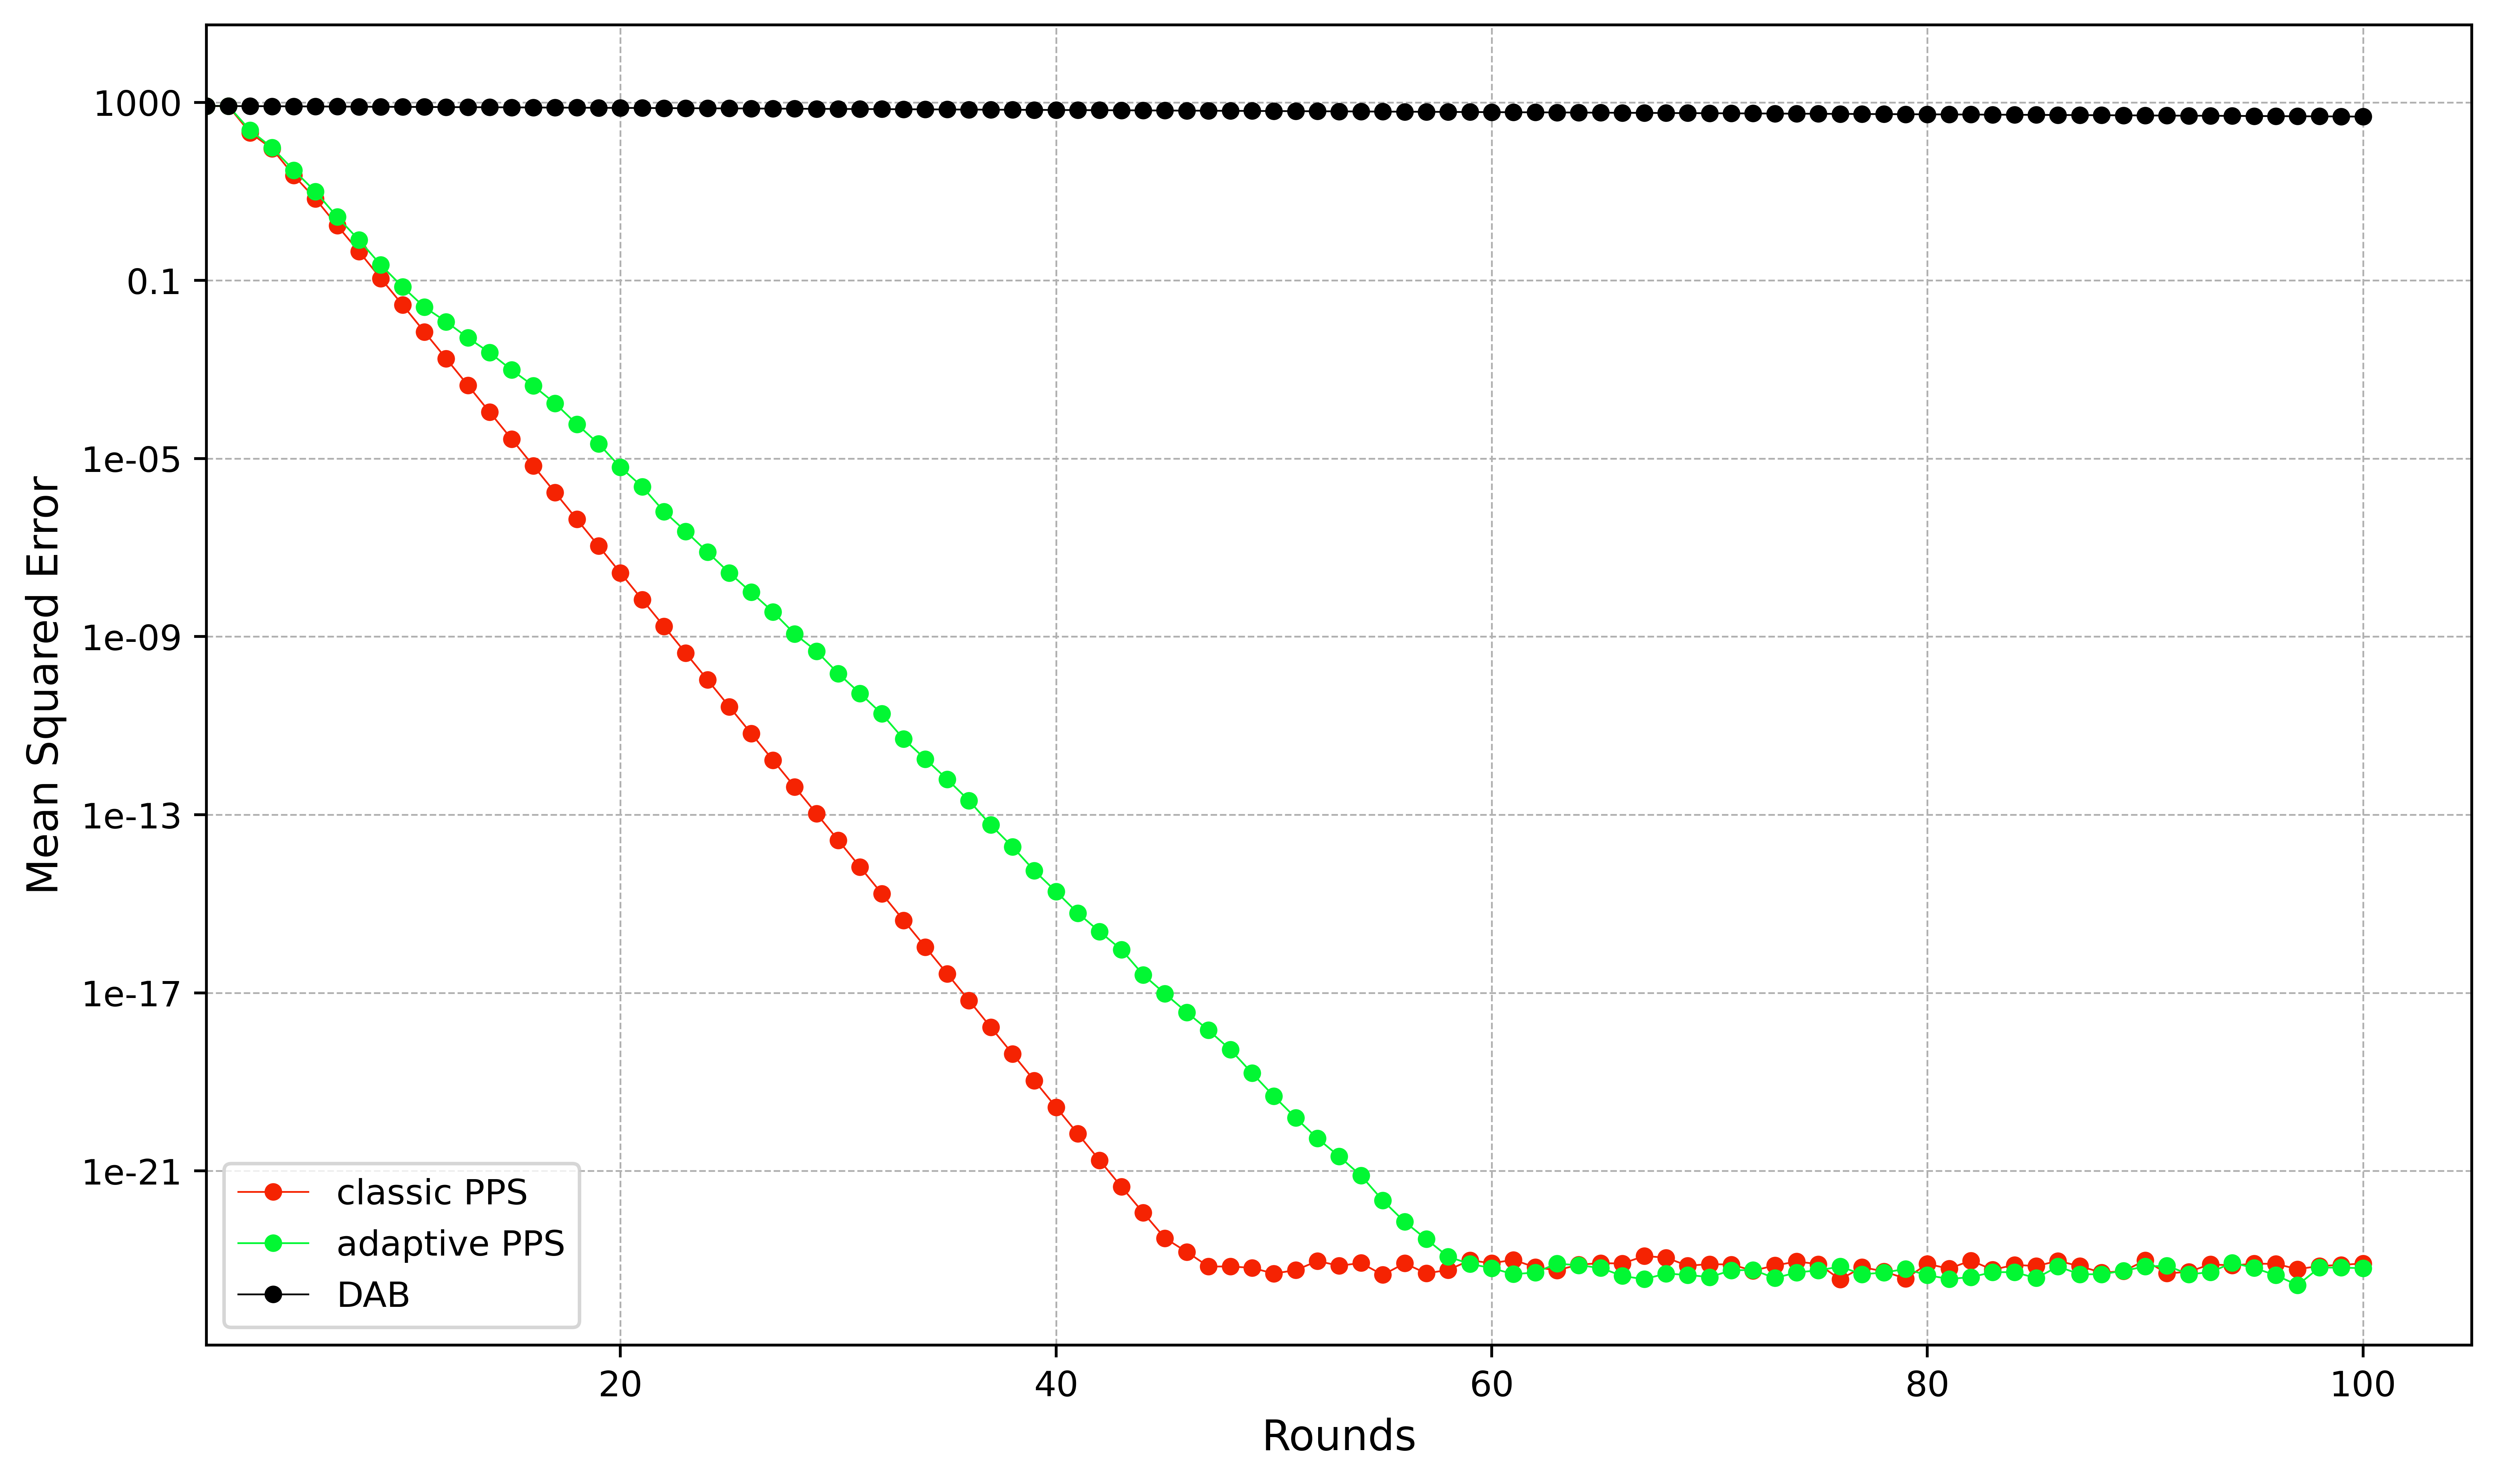
\includegraphics[width=0.49\linewidth]{figures/Simulation_outcomes/StarGraph/DAB_vs_PPS_SG_r100_n1024_averaged_log.png}}
    \hfil
        \subfloat[]{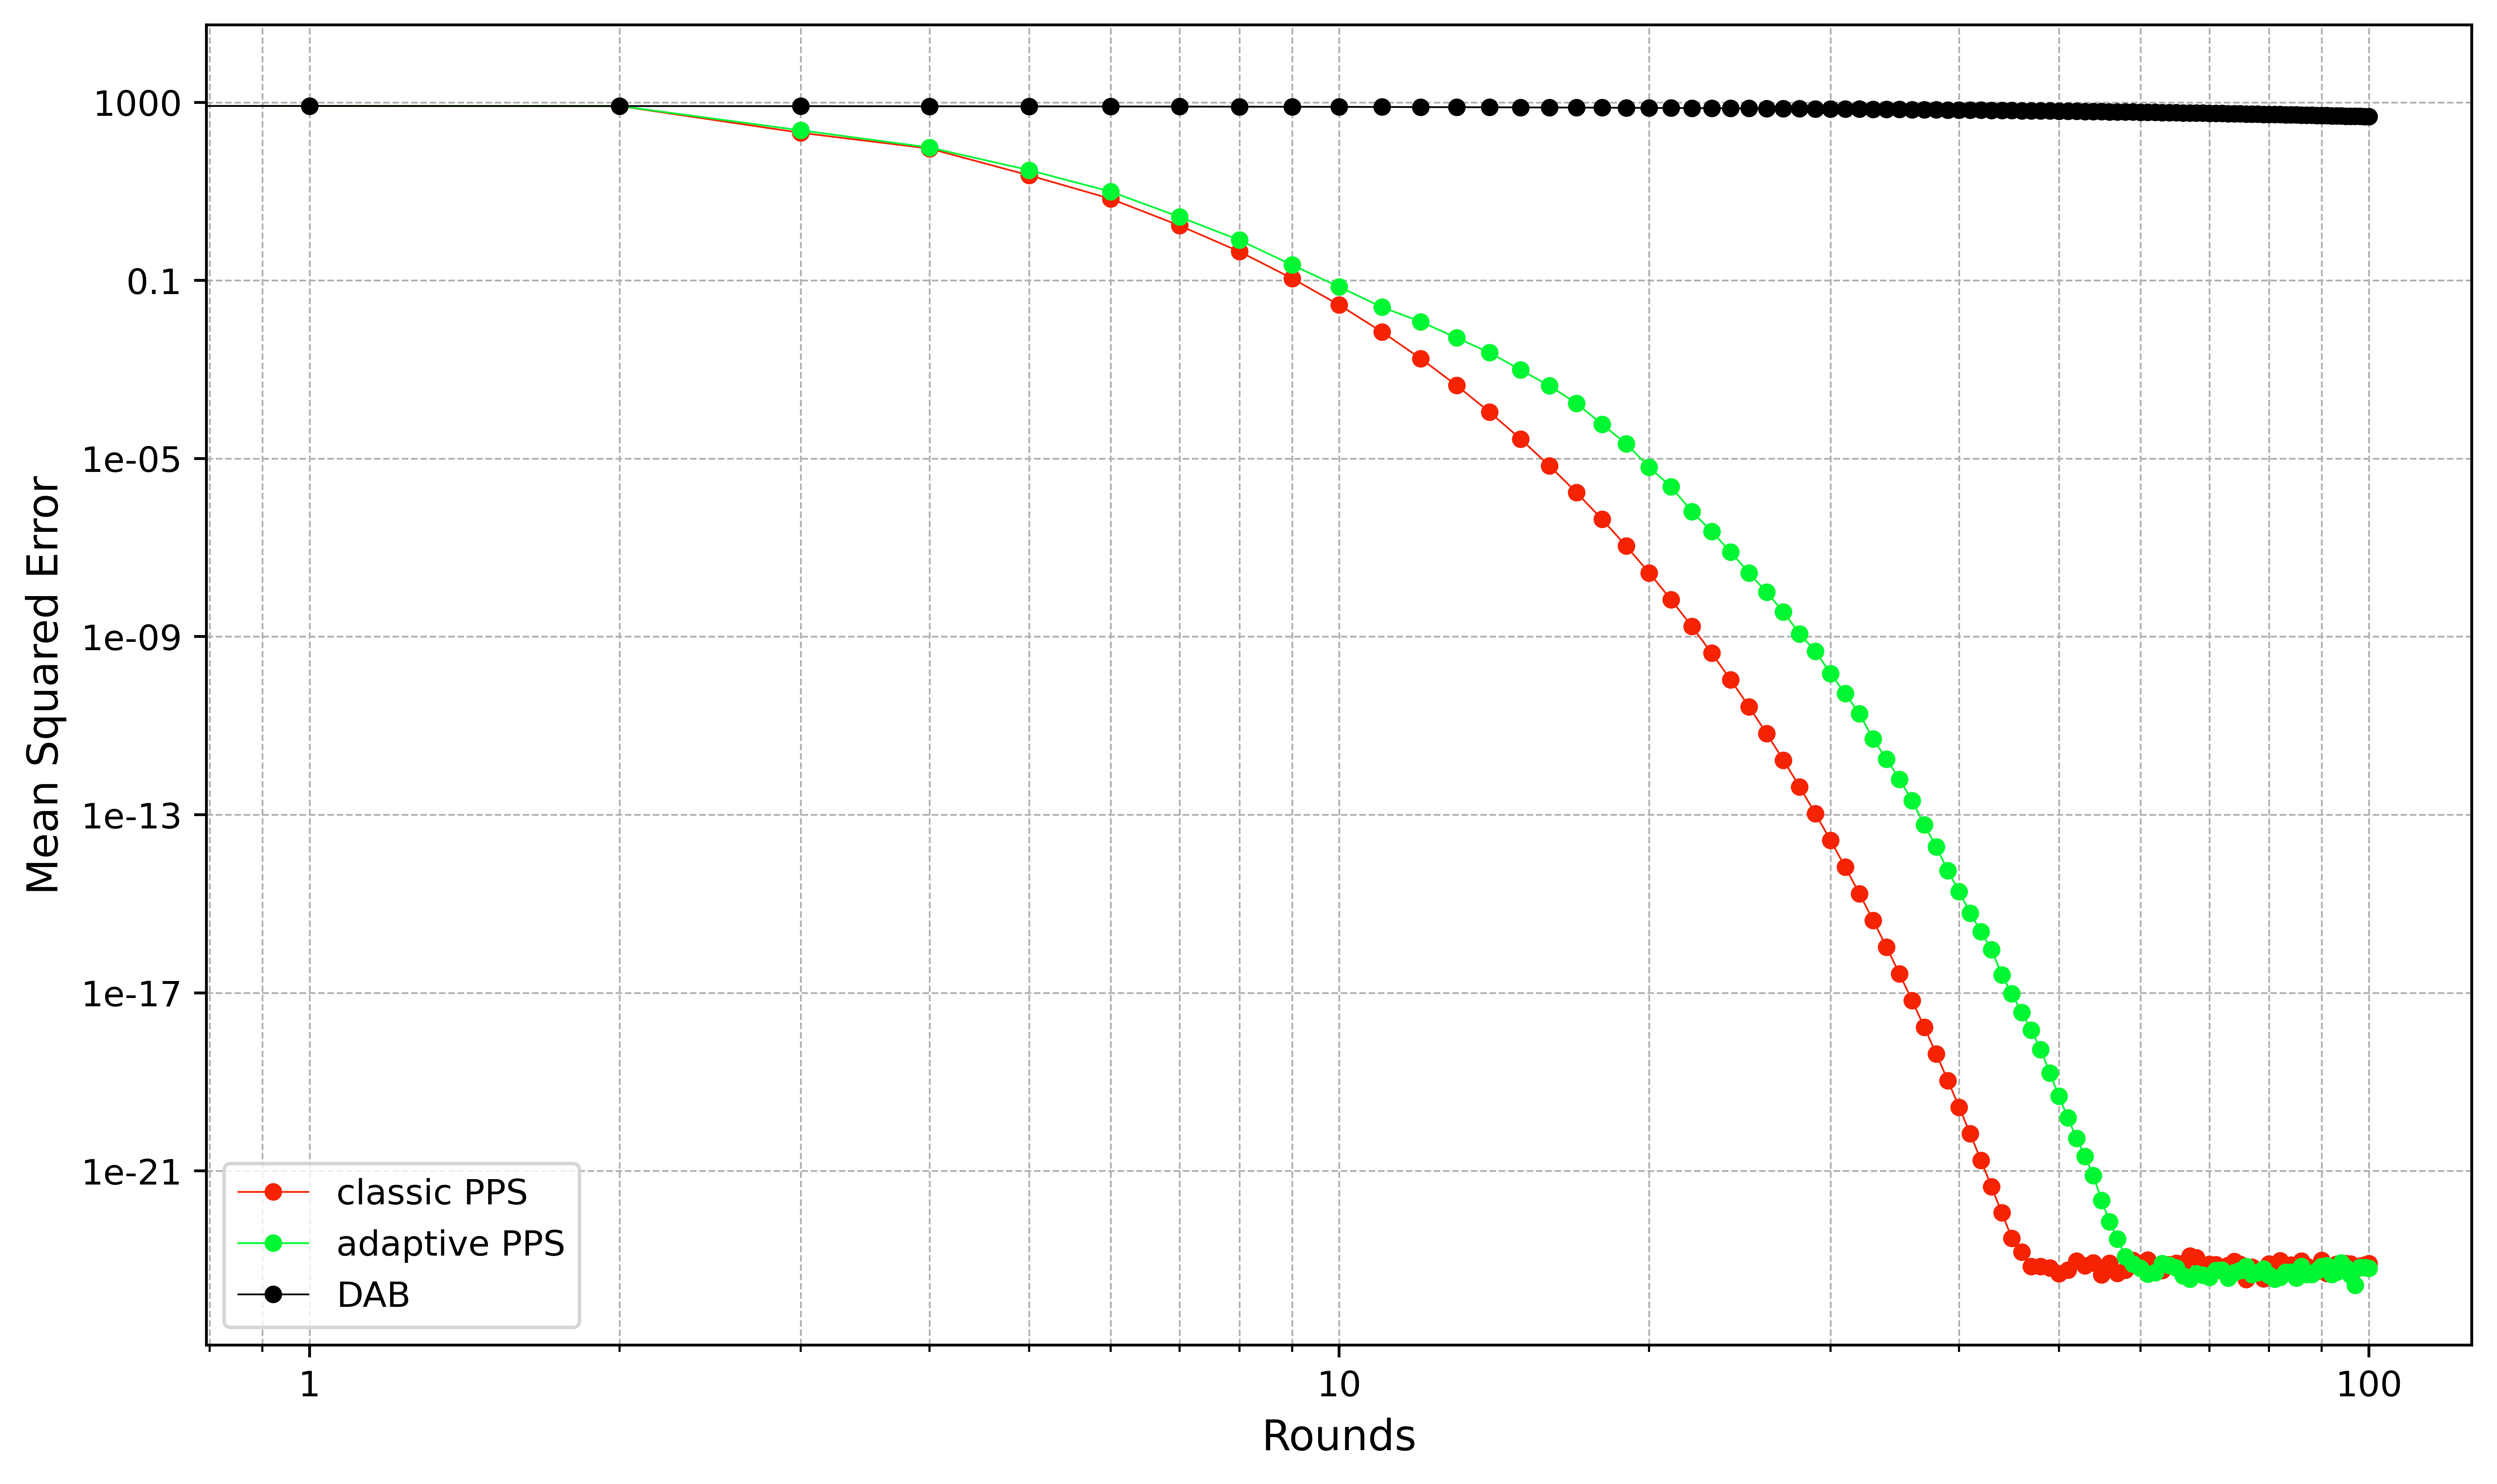
\includegraphics[width=0.49\linewidth]{figures/Simulation_outcomes/StarGraph/DAB_vs_PPS_SG_r100_n1024_averaged_loglog.png}}
    \caption{Star graph - mean squared error per rounds - log-linear and log-log}
        \label{fig:stargraphMSEperRoundLogLog}
\end{figure}

\begin{figure}[!ht]
    \centering
        \subfloat[]{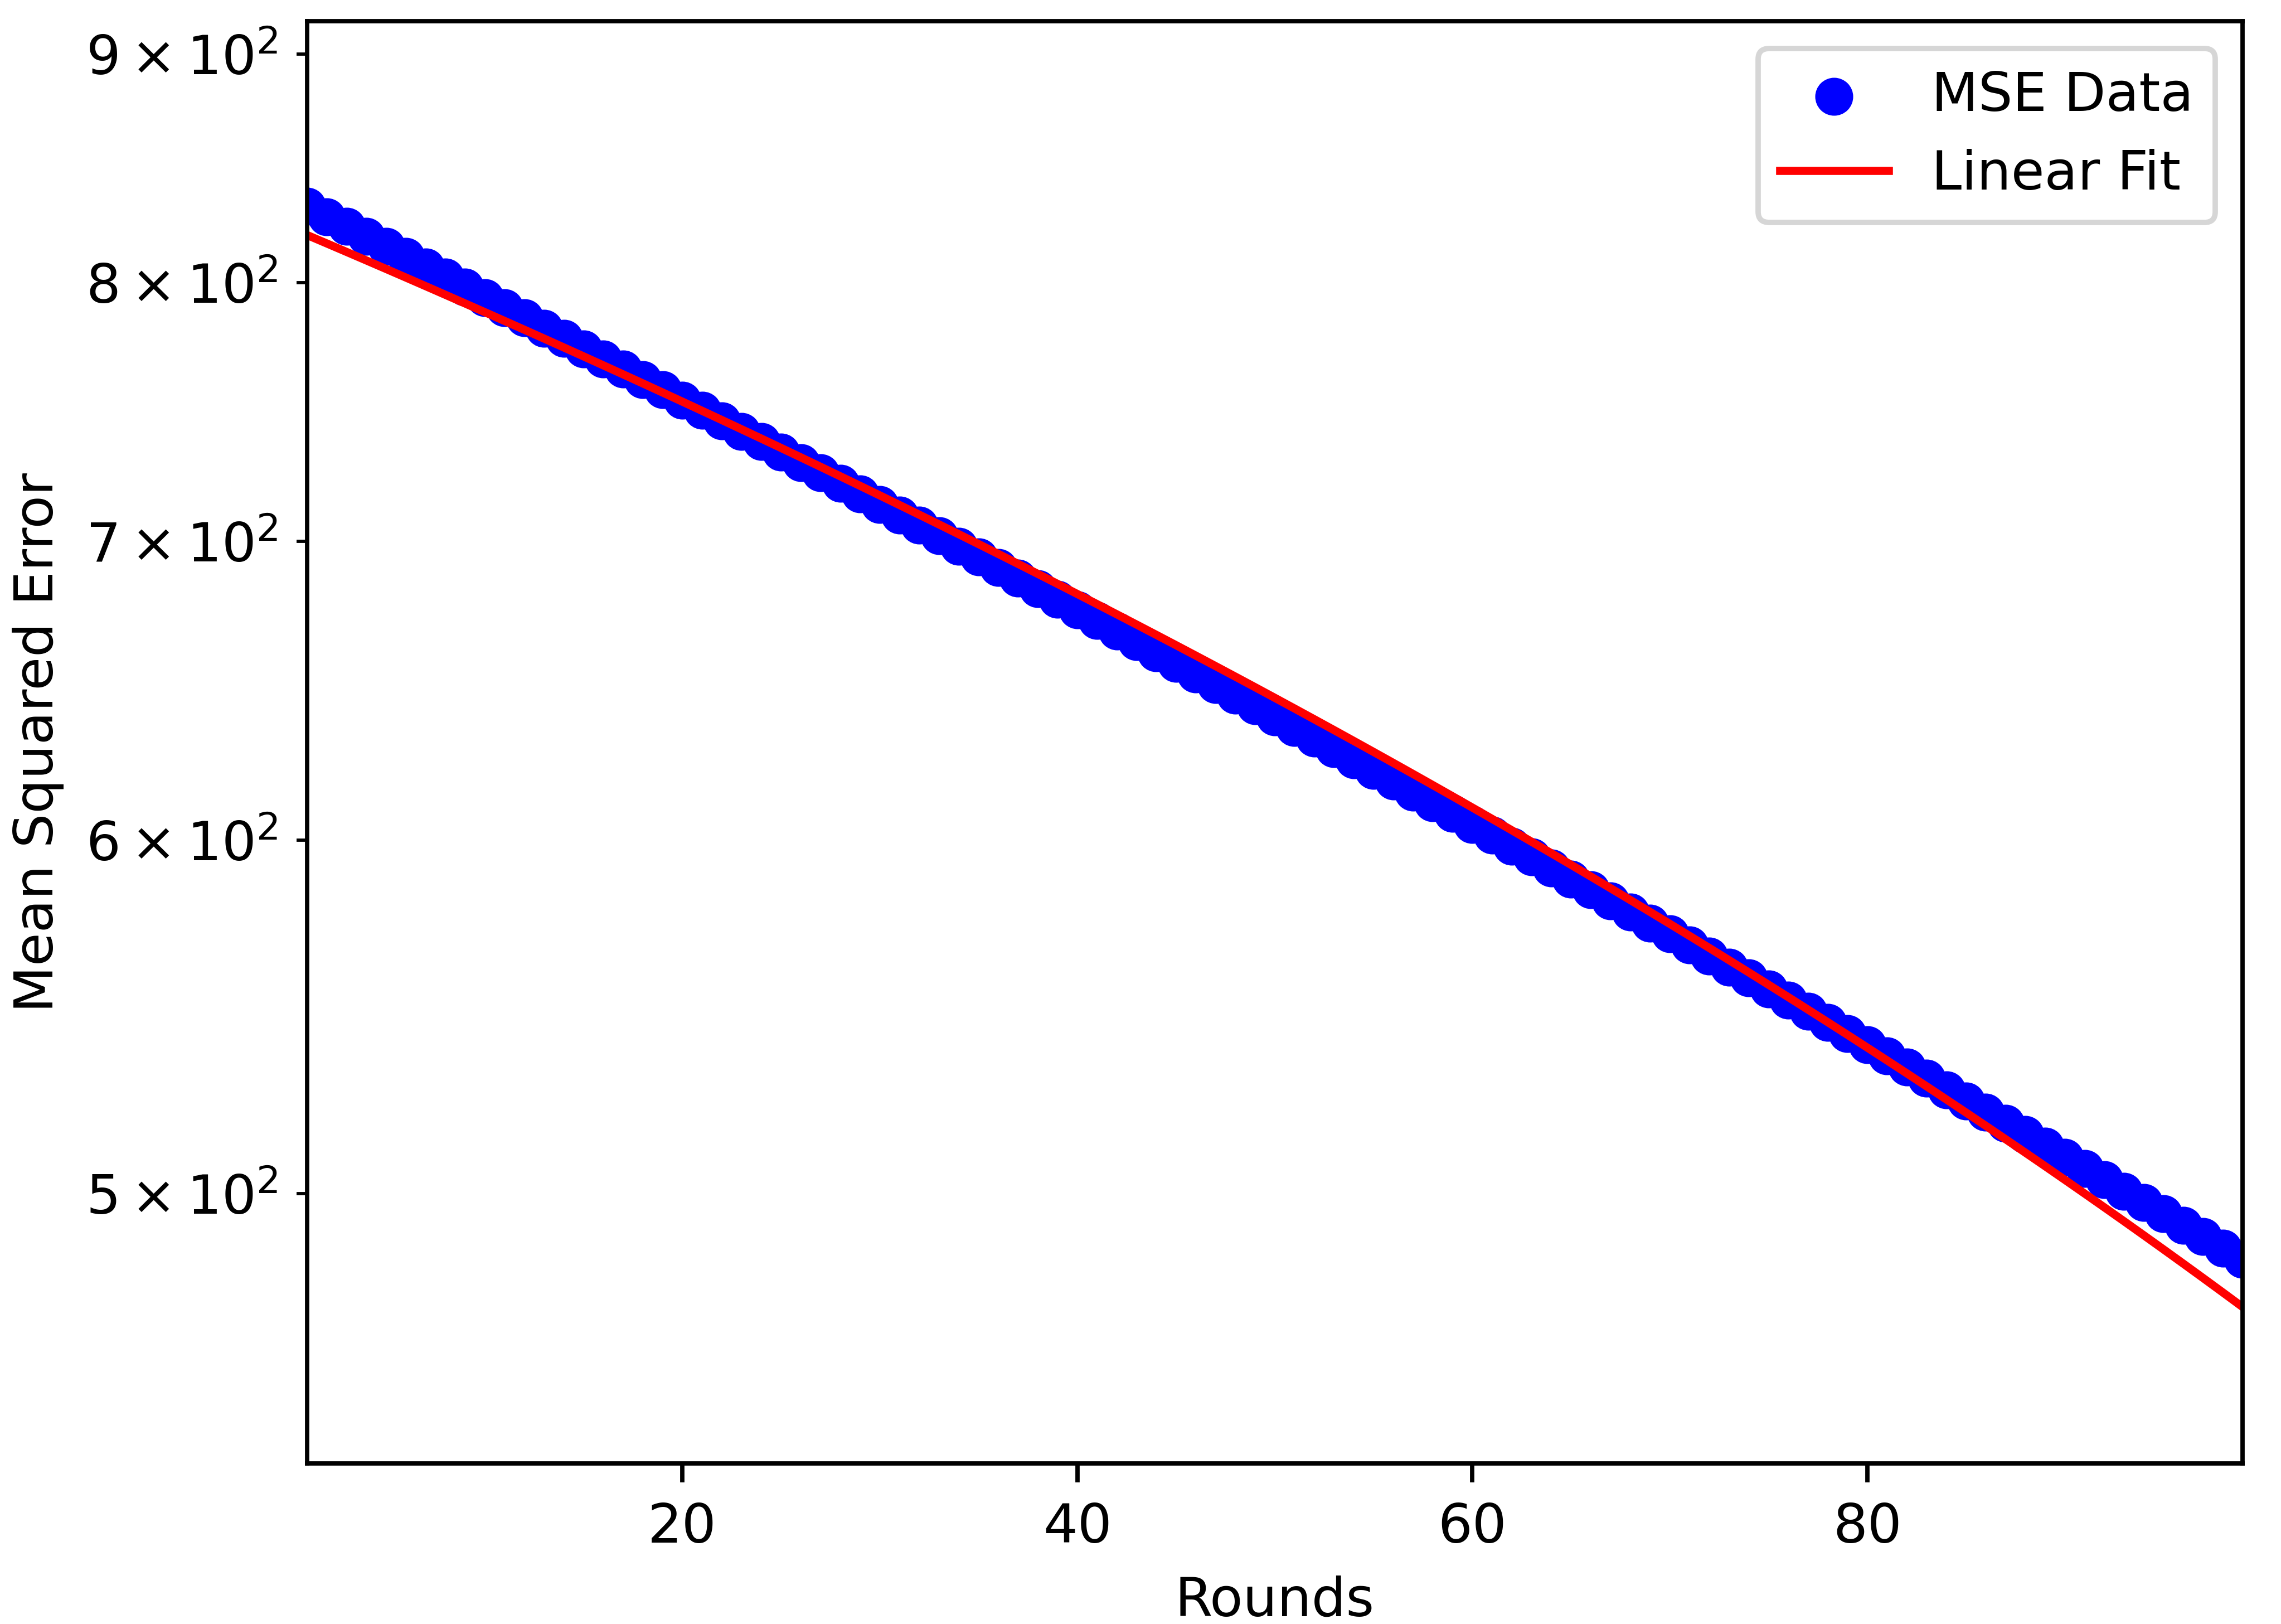
\includegraphics[width=0.49\linewidth]{figures/Simulation_outcomes/StarGraph/DAB/DAB_modelfitting_rounds_99_model_0.png}}
    \hfil
        \subfloat[]{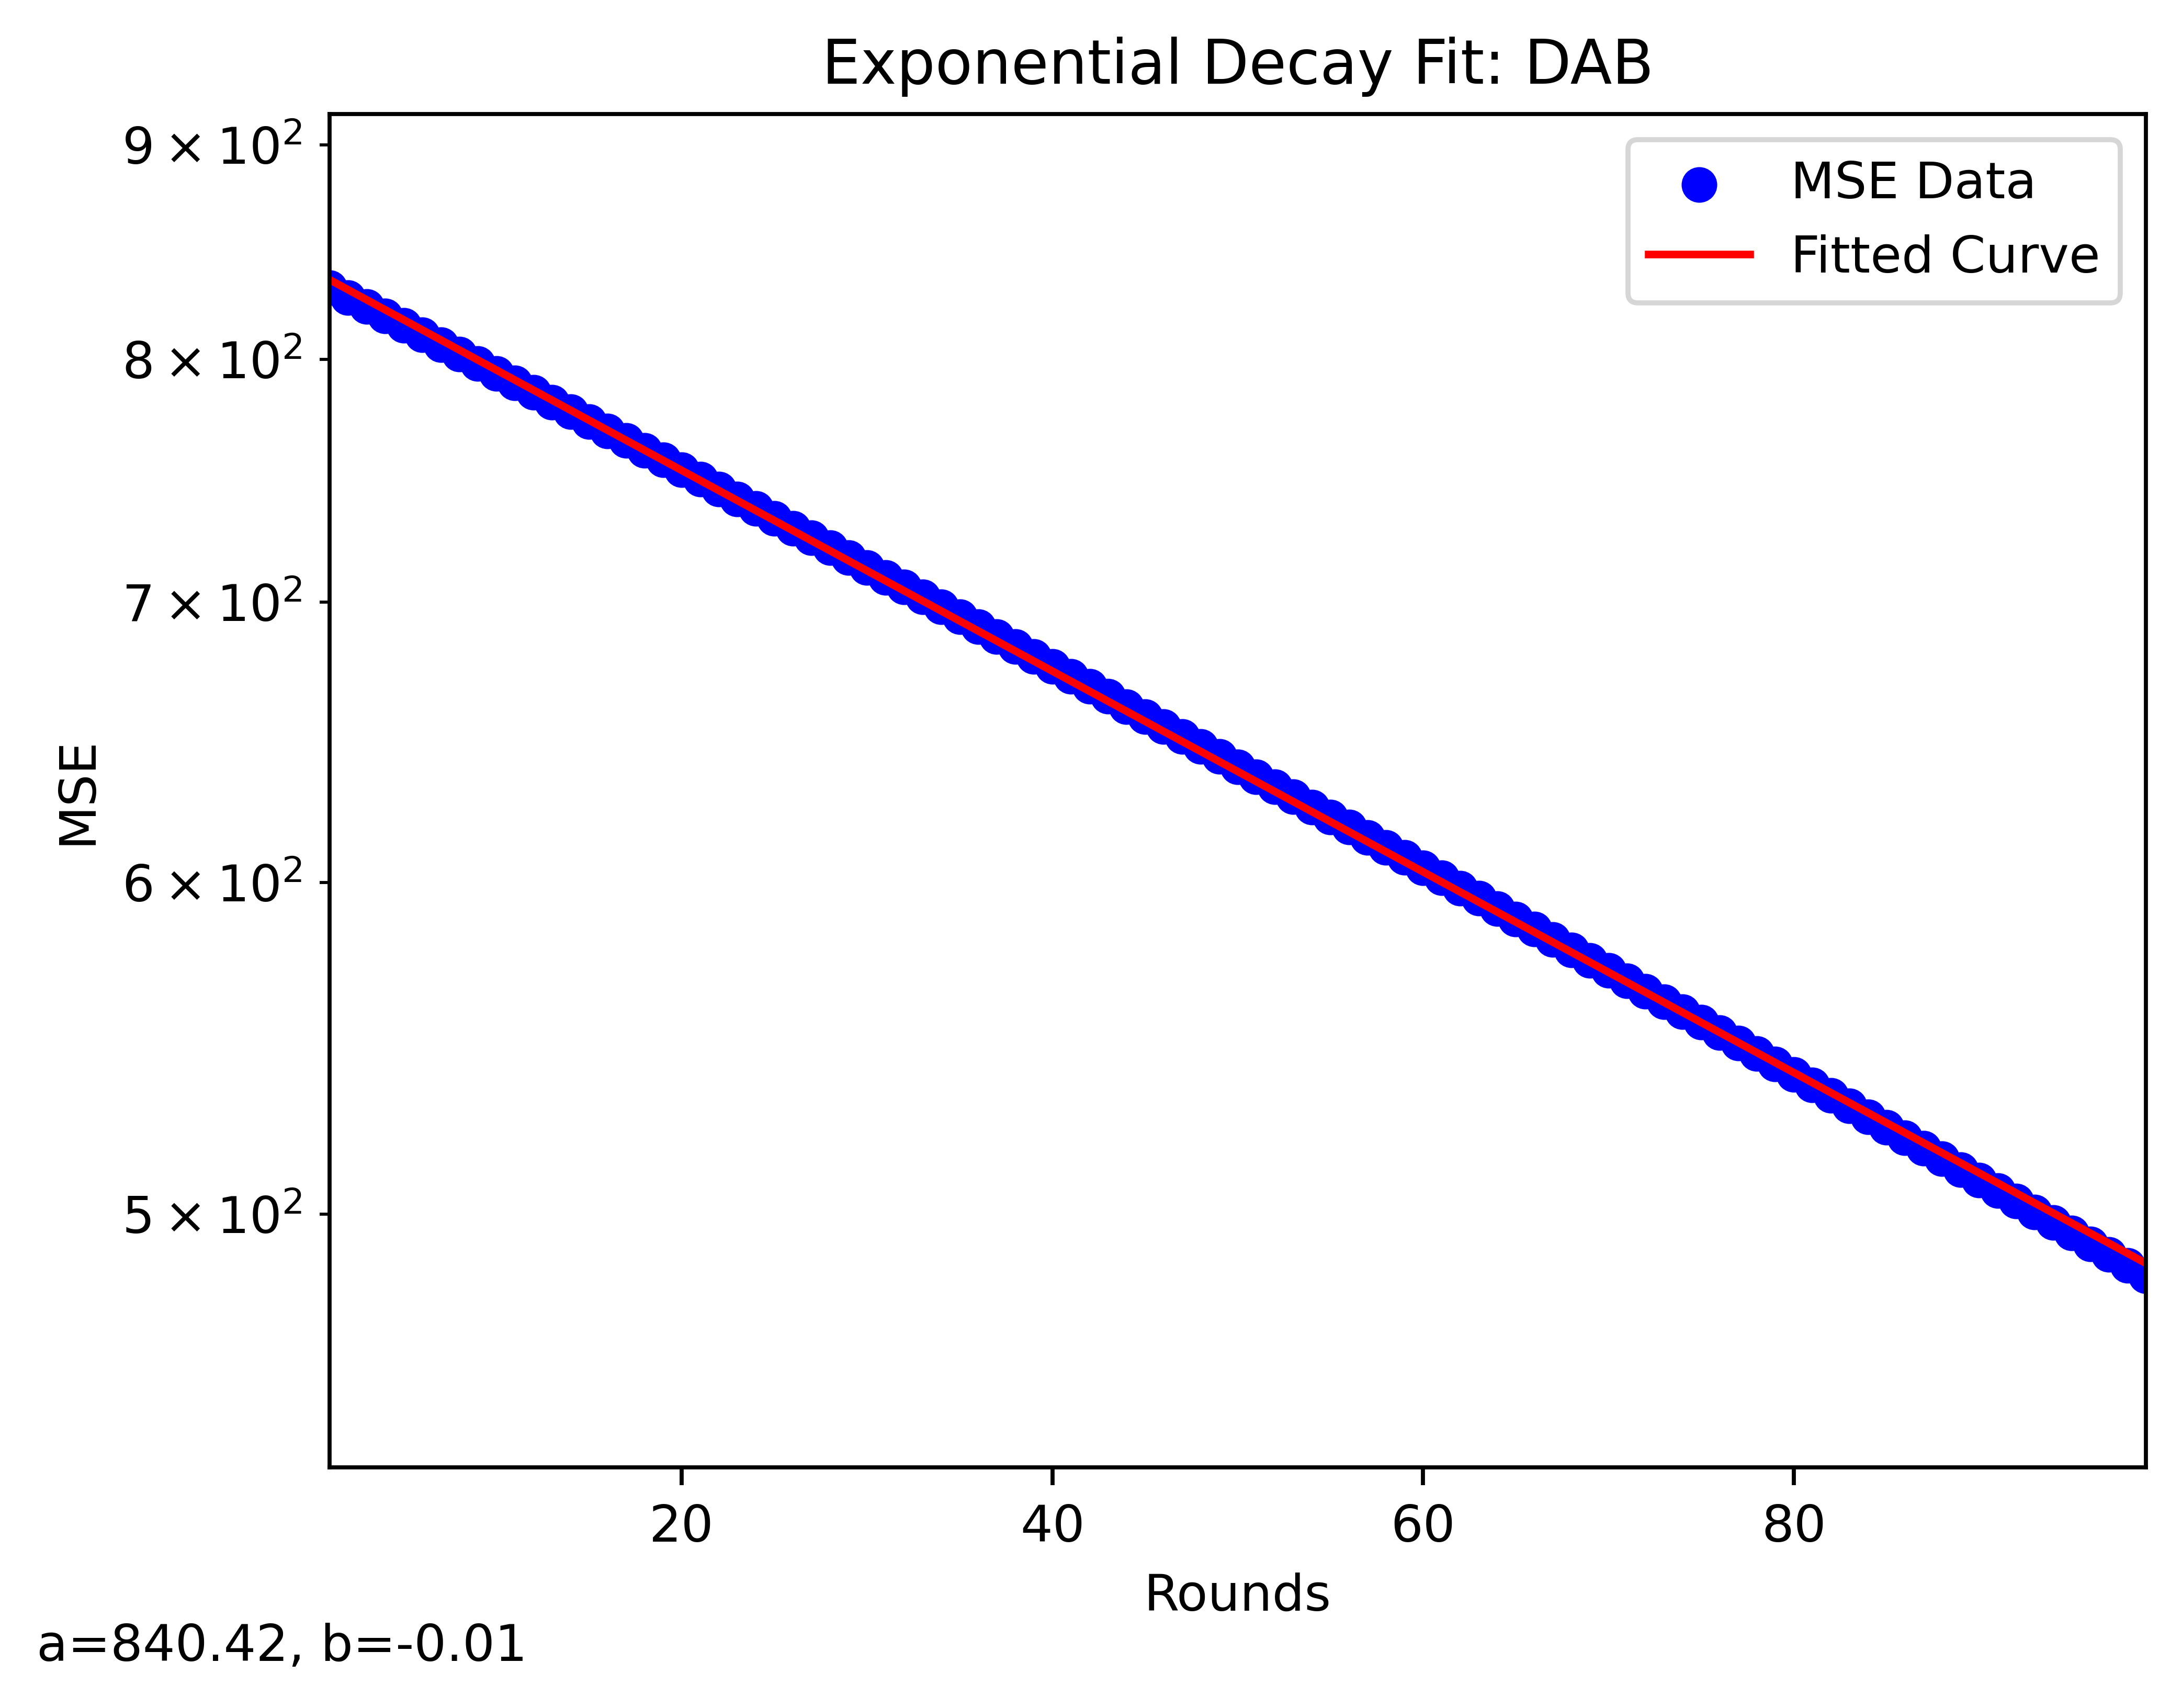
\includegraphics[width=0.49\linewidth]{figures/Simulation_outcomes/StarGraph/DAB/DAB_modelfitting_rounds_99_model_1.png}}
    \caption{Star graph - linear and exponential regression - DAB}
        \label{fig:dabStarModelFit}
\end{figure}

\begin{figure}[]
    \centering
    \scalebox{0.8}{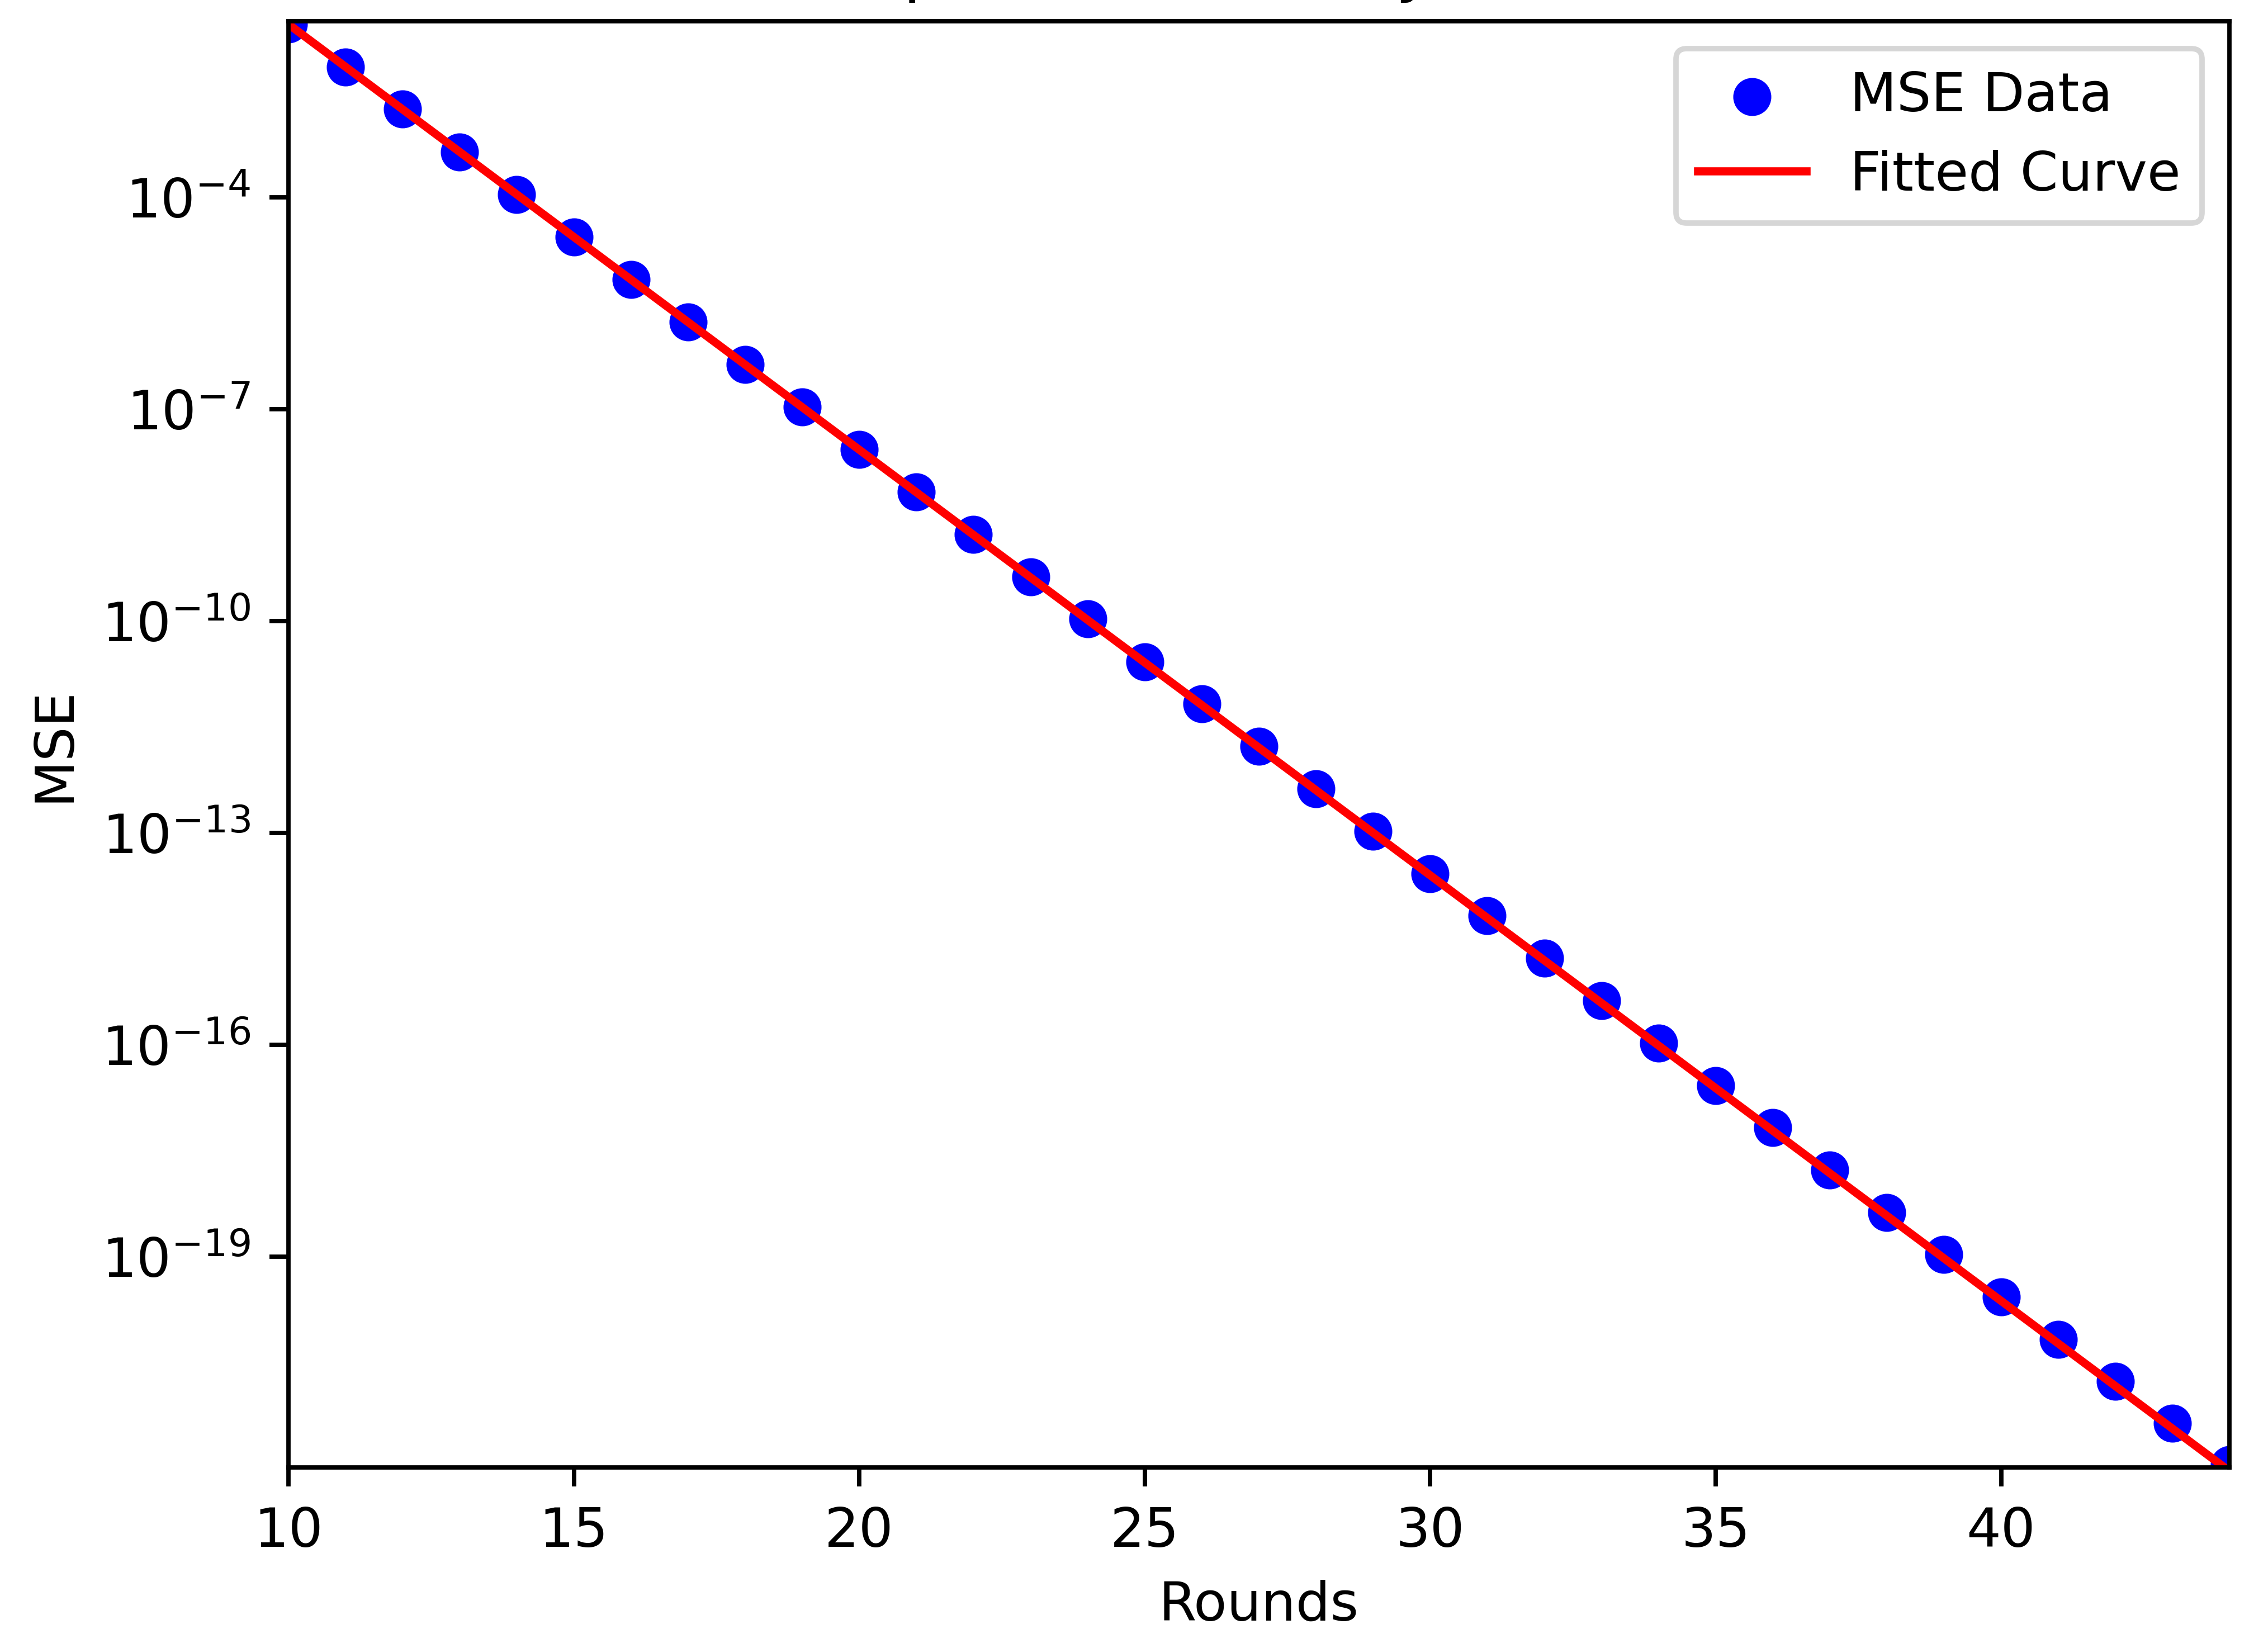
\includegraphics{figures/Simulation_outcomes/StarGraph/PPS/PPS_modelfitting_rounds_44_model_1.png}}
    \caption{Star graph - exponential regression fit - PPS}
    \label{fig:ppsStarModelFit}
\end{figure}
\begin{figure}[]
    \centering
    \scalebox{0.8}{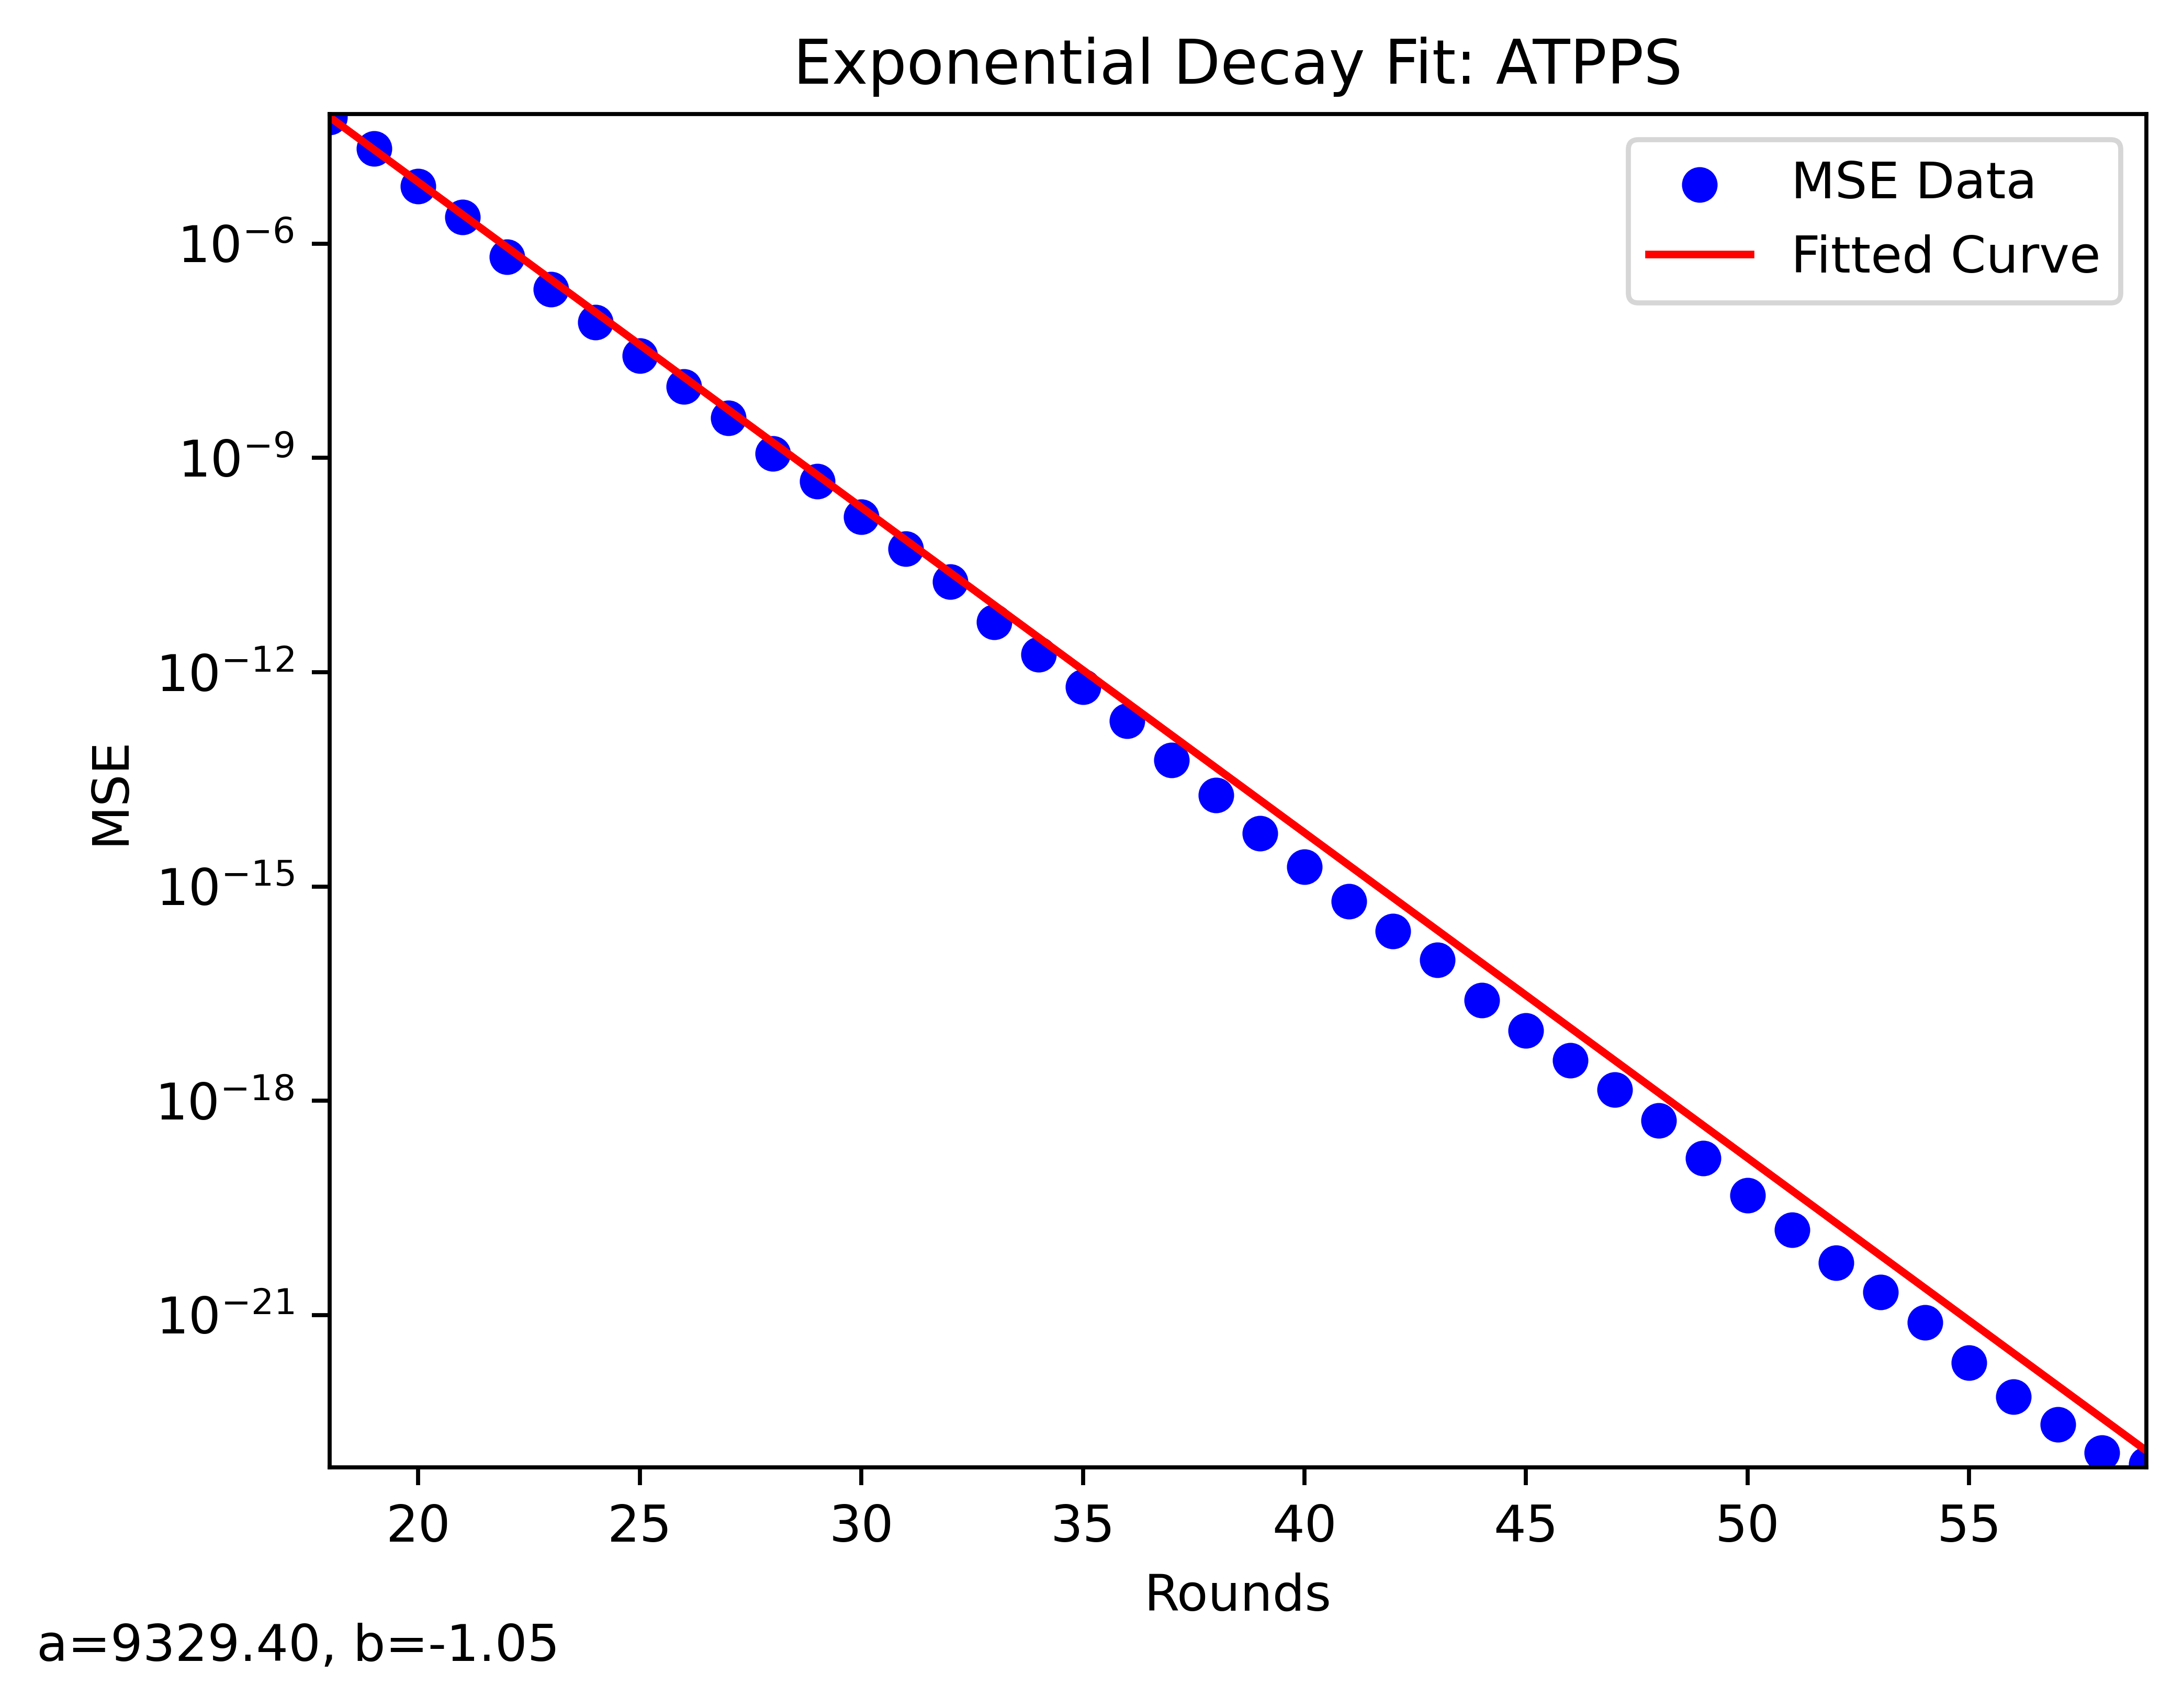
\includegraphics{figures/Simulation_outcomes/StarGraph/ATPPS/ATPPS_modelfitting_rounds_59_model_1.png}}
    \caption{Star graph - exponential regression fit - ATPPS}
    \label{fig:atppsStarModelFit}
\end{figure}

\begin{figure}[!ht]
    \centering
        \subfloat[]{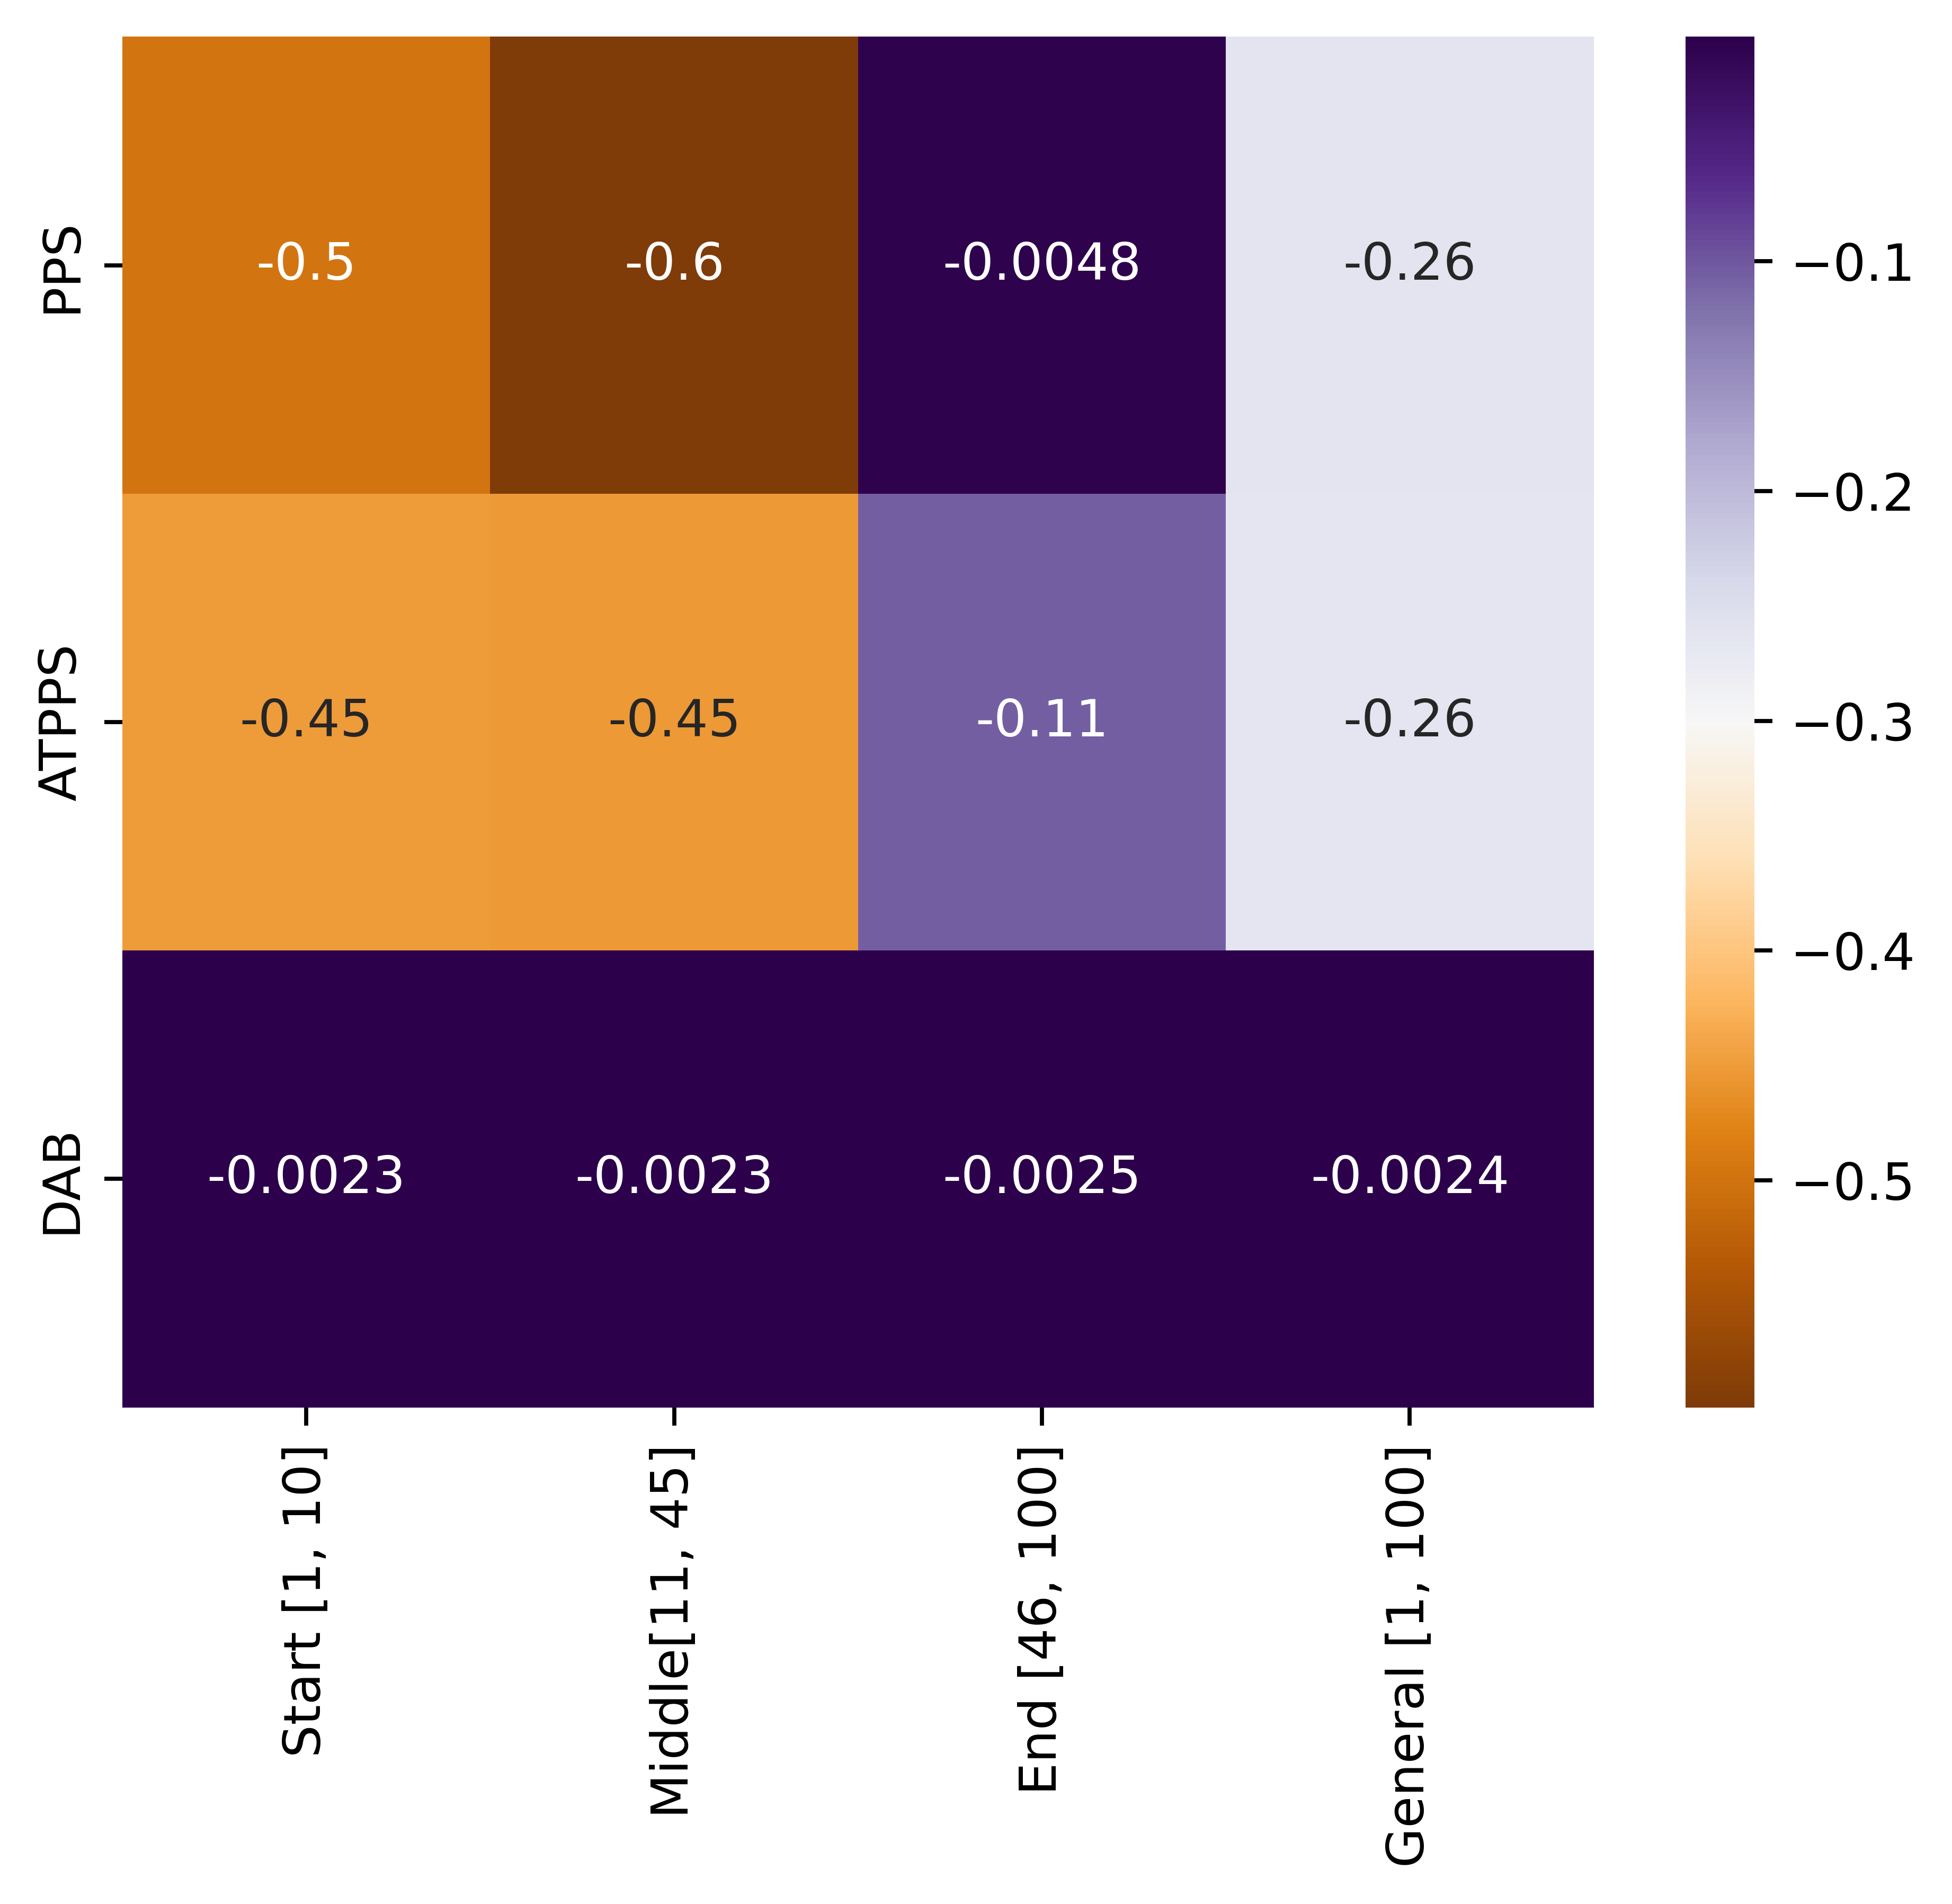
\includegraphics[width=0.49\linewidth]{figures/Simulation_outcomes/StarGraph/DAB_vs_PPS_vs_ATPPS_slopesheatmap_100rounds_log_linear.png}}
    \hfil
        \subfloat[]{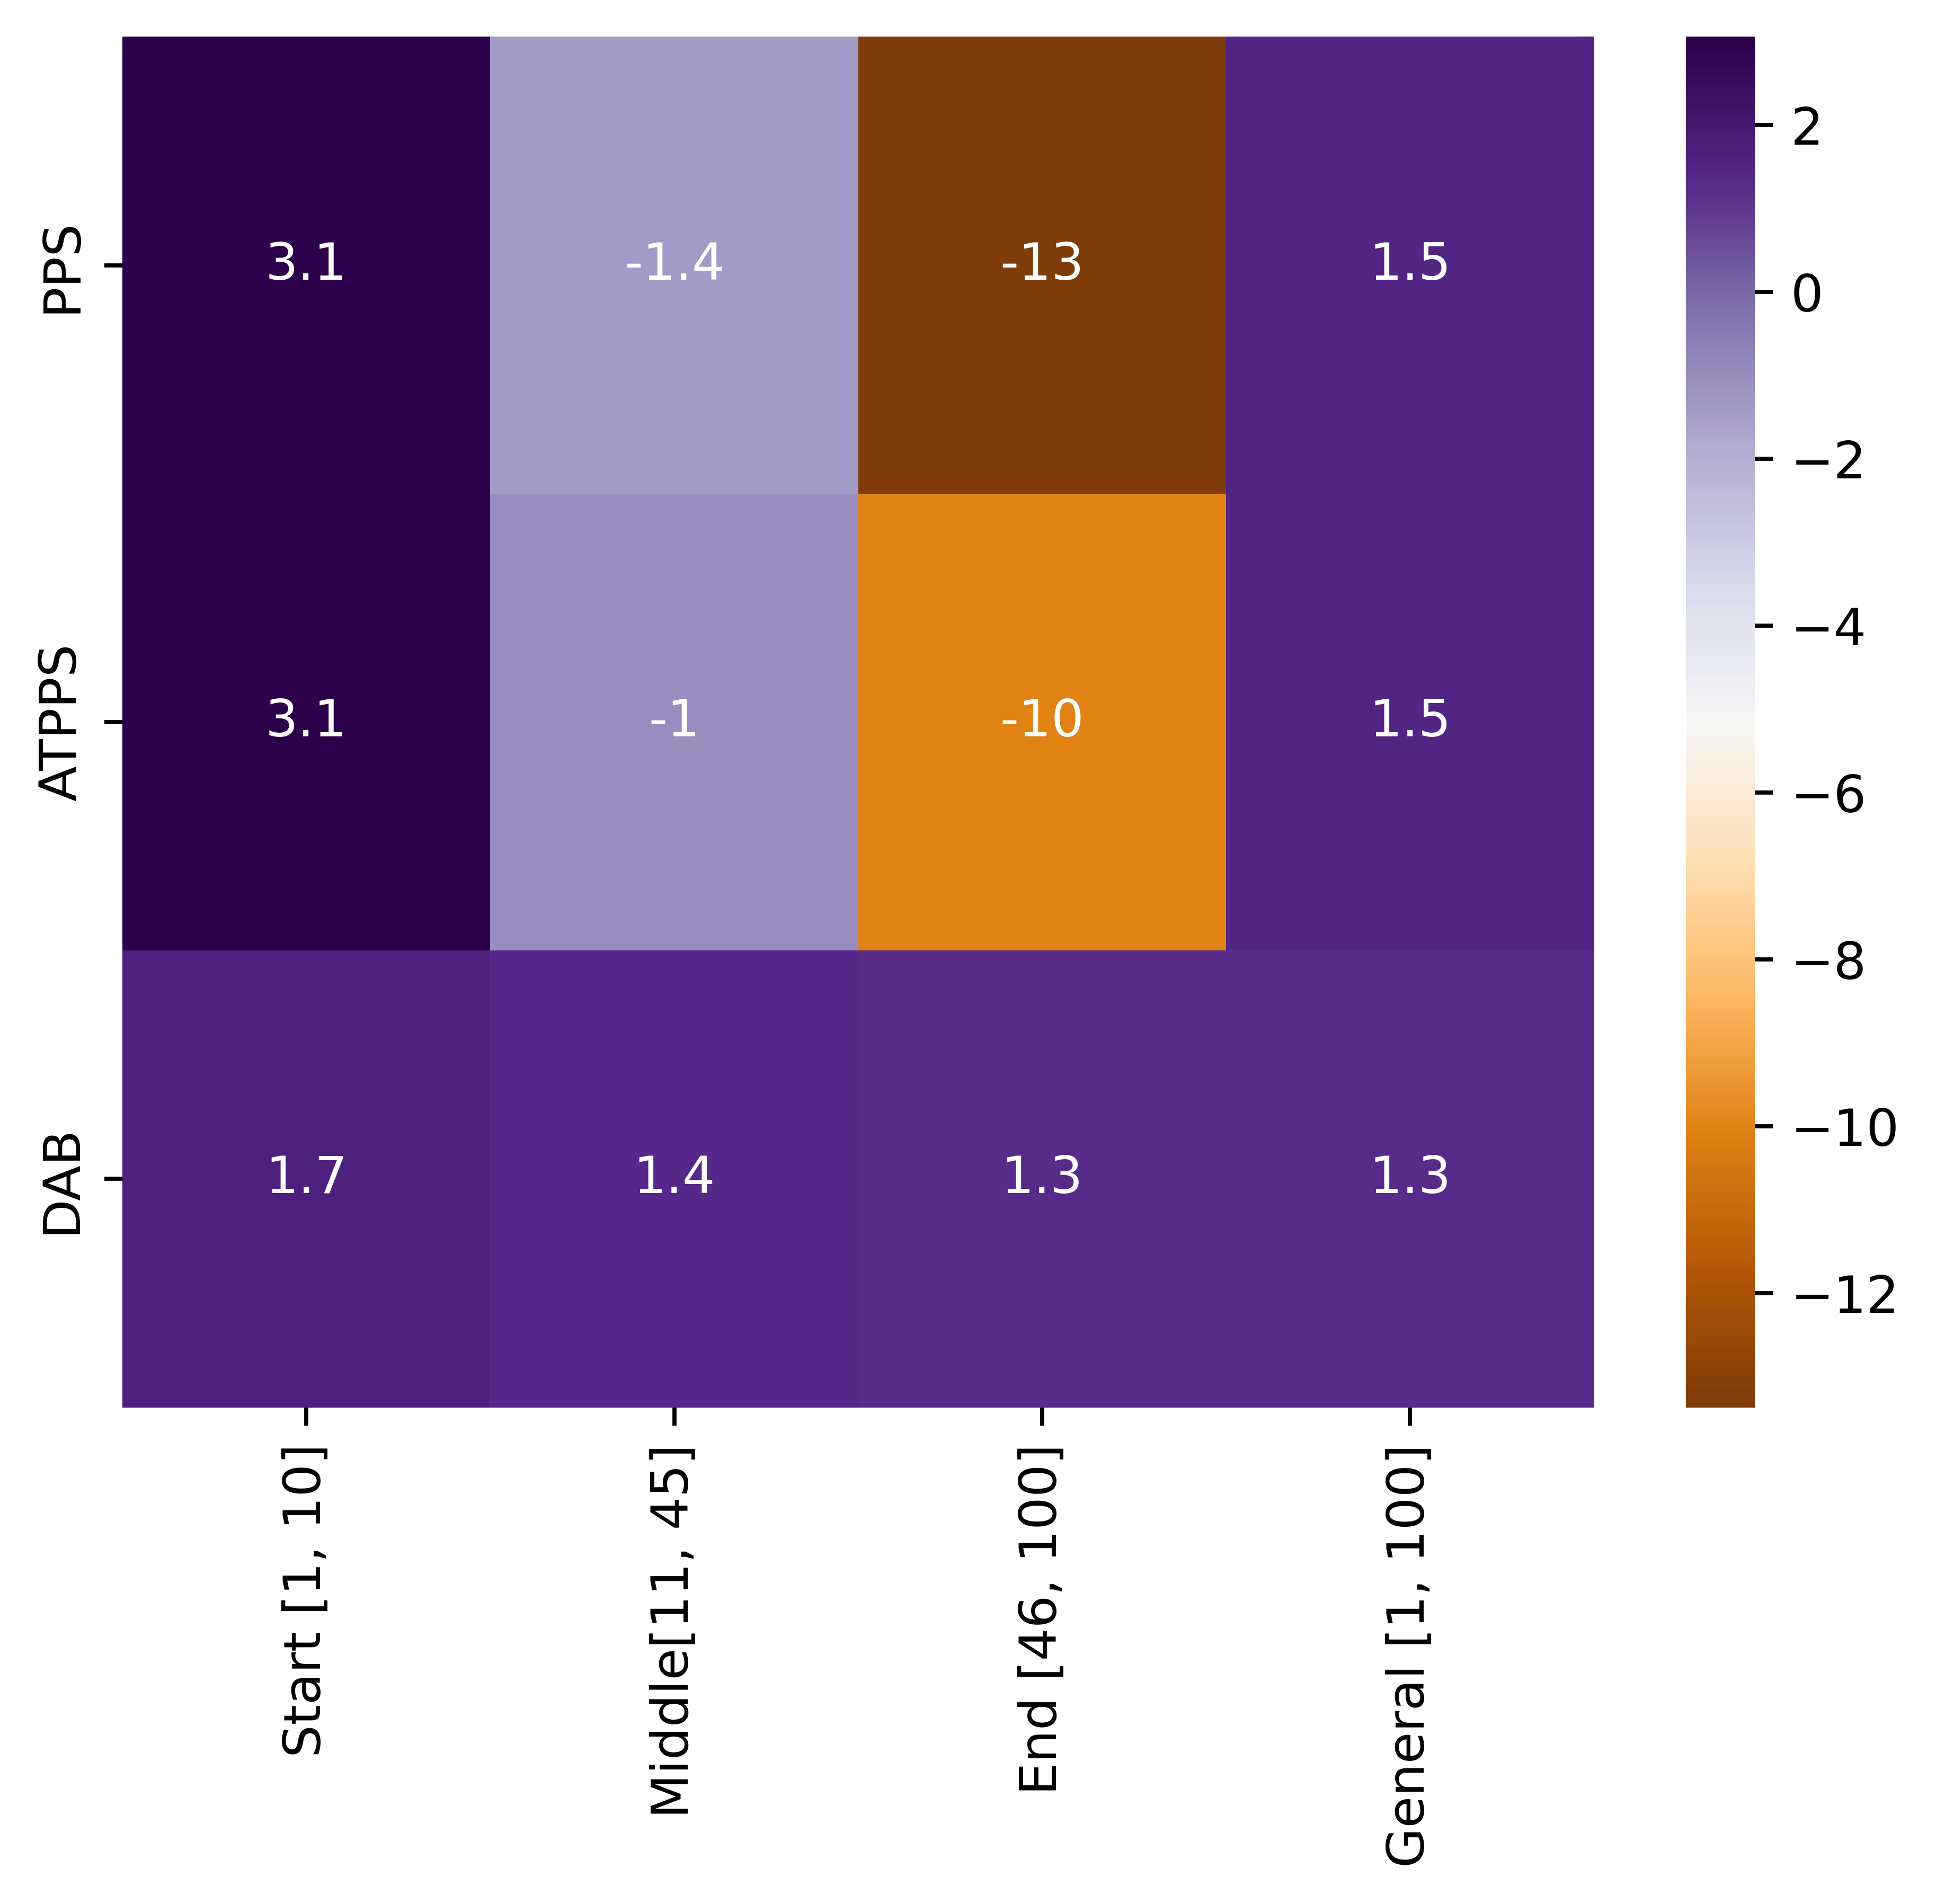
\includegraphics[width=0.49\linewidth]{figures/Simulation_outcomes/StarGraph/DAB_vs_PPS_vs_ATPPS_slopesheatmap_100rounds_log_log.png}}
    \caption{Star graph - heat map of slopes per region - log-linear and log-log}
        \label{fig:stargraphslopes}
\end{figure}

\section{Ring Graph}\label{sec:ringgraph}
For the Ring graph $R_{1024}$, the DAB curve in figure \ref{fig:ringgraphMSEperRoundLogLog} shows the steepest decline in error in the first few rounds of the simulation. The slopes in figure \ref{fig:ringgraphslopes}, represent the exponents in the power-law relationship between the MSE and $r$. The slope of the first 10 rounds is $-1.1$ for the DAB curve compared to $-0.94 \pm 0.1$ for each Push-Pull Sum-based algorithm. The slopes decrease for all three algorithms to $-0.53 \pm 0.3$ in the middle region and remain at these values for the end region. The near-overlap of PPS and ATPPS across the 100 rounds of simulation suggests that the adaptive mechanism provides limited additional benefit in a Ring graph, where selecting a random neighbor might already target an optimal load transfer partner. In a Ring topology, each node only interacts with its two immediate neighbors. The adaptive threshold mechanism relies on significant load differences between nodes to trigger transfers, but in a Ring graph, local load differences might not be significant enough to make the threshold mechanism advantageous. For the PPS, every node communicates with its neighbors in every round. This constant exchange ensures rapid propagation of load. The adaptive threshold might reduce some of these exchanges. However, in a Ring graph, where the network diameter is large, reducing communication might delay convergence rather than improve it. The threshold mechanism could therefore counteract its own benefits and limit its advantage over the PPS. The DAB performs better in this scenario since it always interacts with the optimal partner to exchange loads. The benefit of randomness vanishes for a network topology where each node only has two neighbors, and a deterministic approach actually performs better.

The MSE data from each algorithm's simulations were fitted to a polynomial regression model of degree 4. The best-fit model for the DAB MSE data for rounds 10 to 60 follows the equation:
\begin{align}
    MSE_r=1.72\times 10^{-5}r^{4}-2.30\times 10^{-3}r^{3}+ 0.19r^{2}-5.99r+114.83    
\end{align}
as shown in figure \ref{fig:dabRingModelFit}. For small $r$ the constant term dominates. As the time proceeds and $r$ increases the higher-degree terms influence the behavior of the curve more and more. The MSE data of the PPS is fitted to a fourth-degree polynomial model:
\begin{align}
    MSE_r= 2.99\times 10^{-5}r^{4}-5.0\times 10^{-3}r^{3} + 0.32r^{2} -9.68r + 166.30    
\end{align}
as shown in figure \ref{fig:ppsRingModelFit}. The ATPPS MSE data is also fitted to a fourth-degree polynomial:
\begin{align}
    MSE_r=3.04\times 10^{-5}r^{4}-5.0\times 10^{-3}r^{3} + 0.32r^{2}-9.64r+161.86    
\end{align}
as depicted in figure \ref{fig:atppsRingModelFit}. The polynomial fit suggests that MSE reduction slows down over time.

\begin{figure}[]
    \centering
    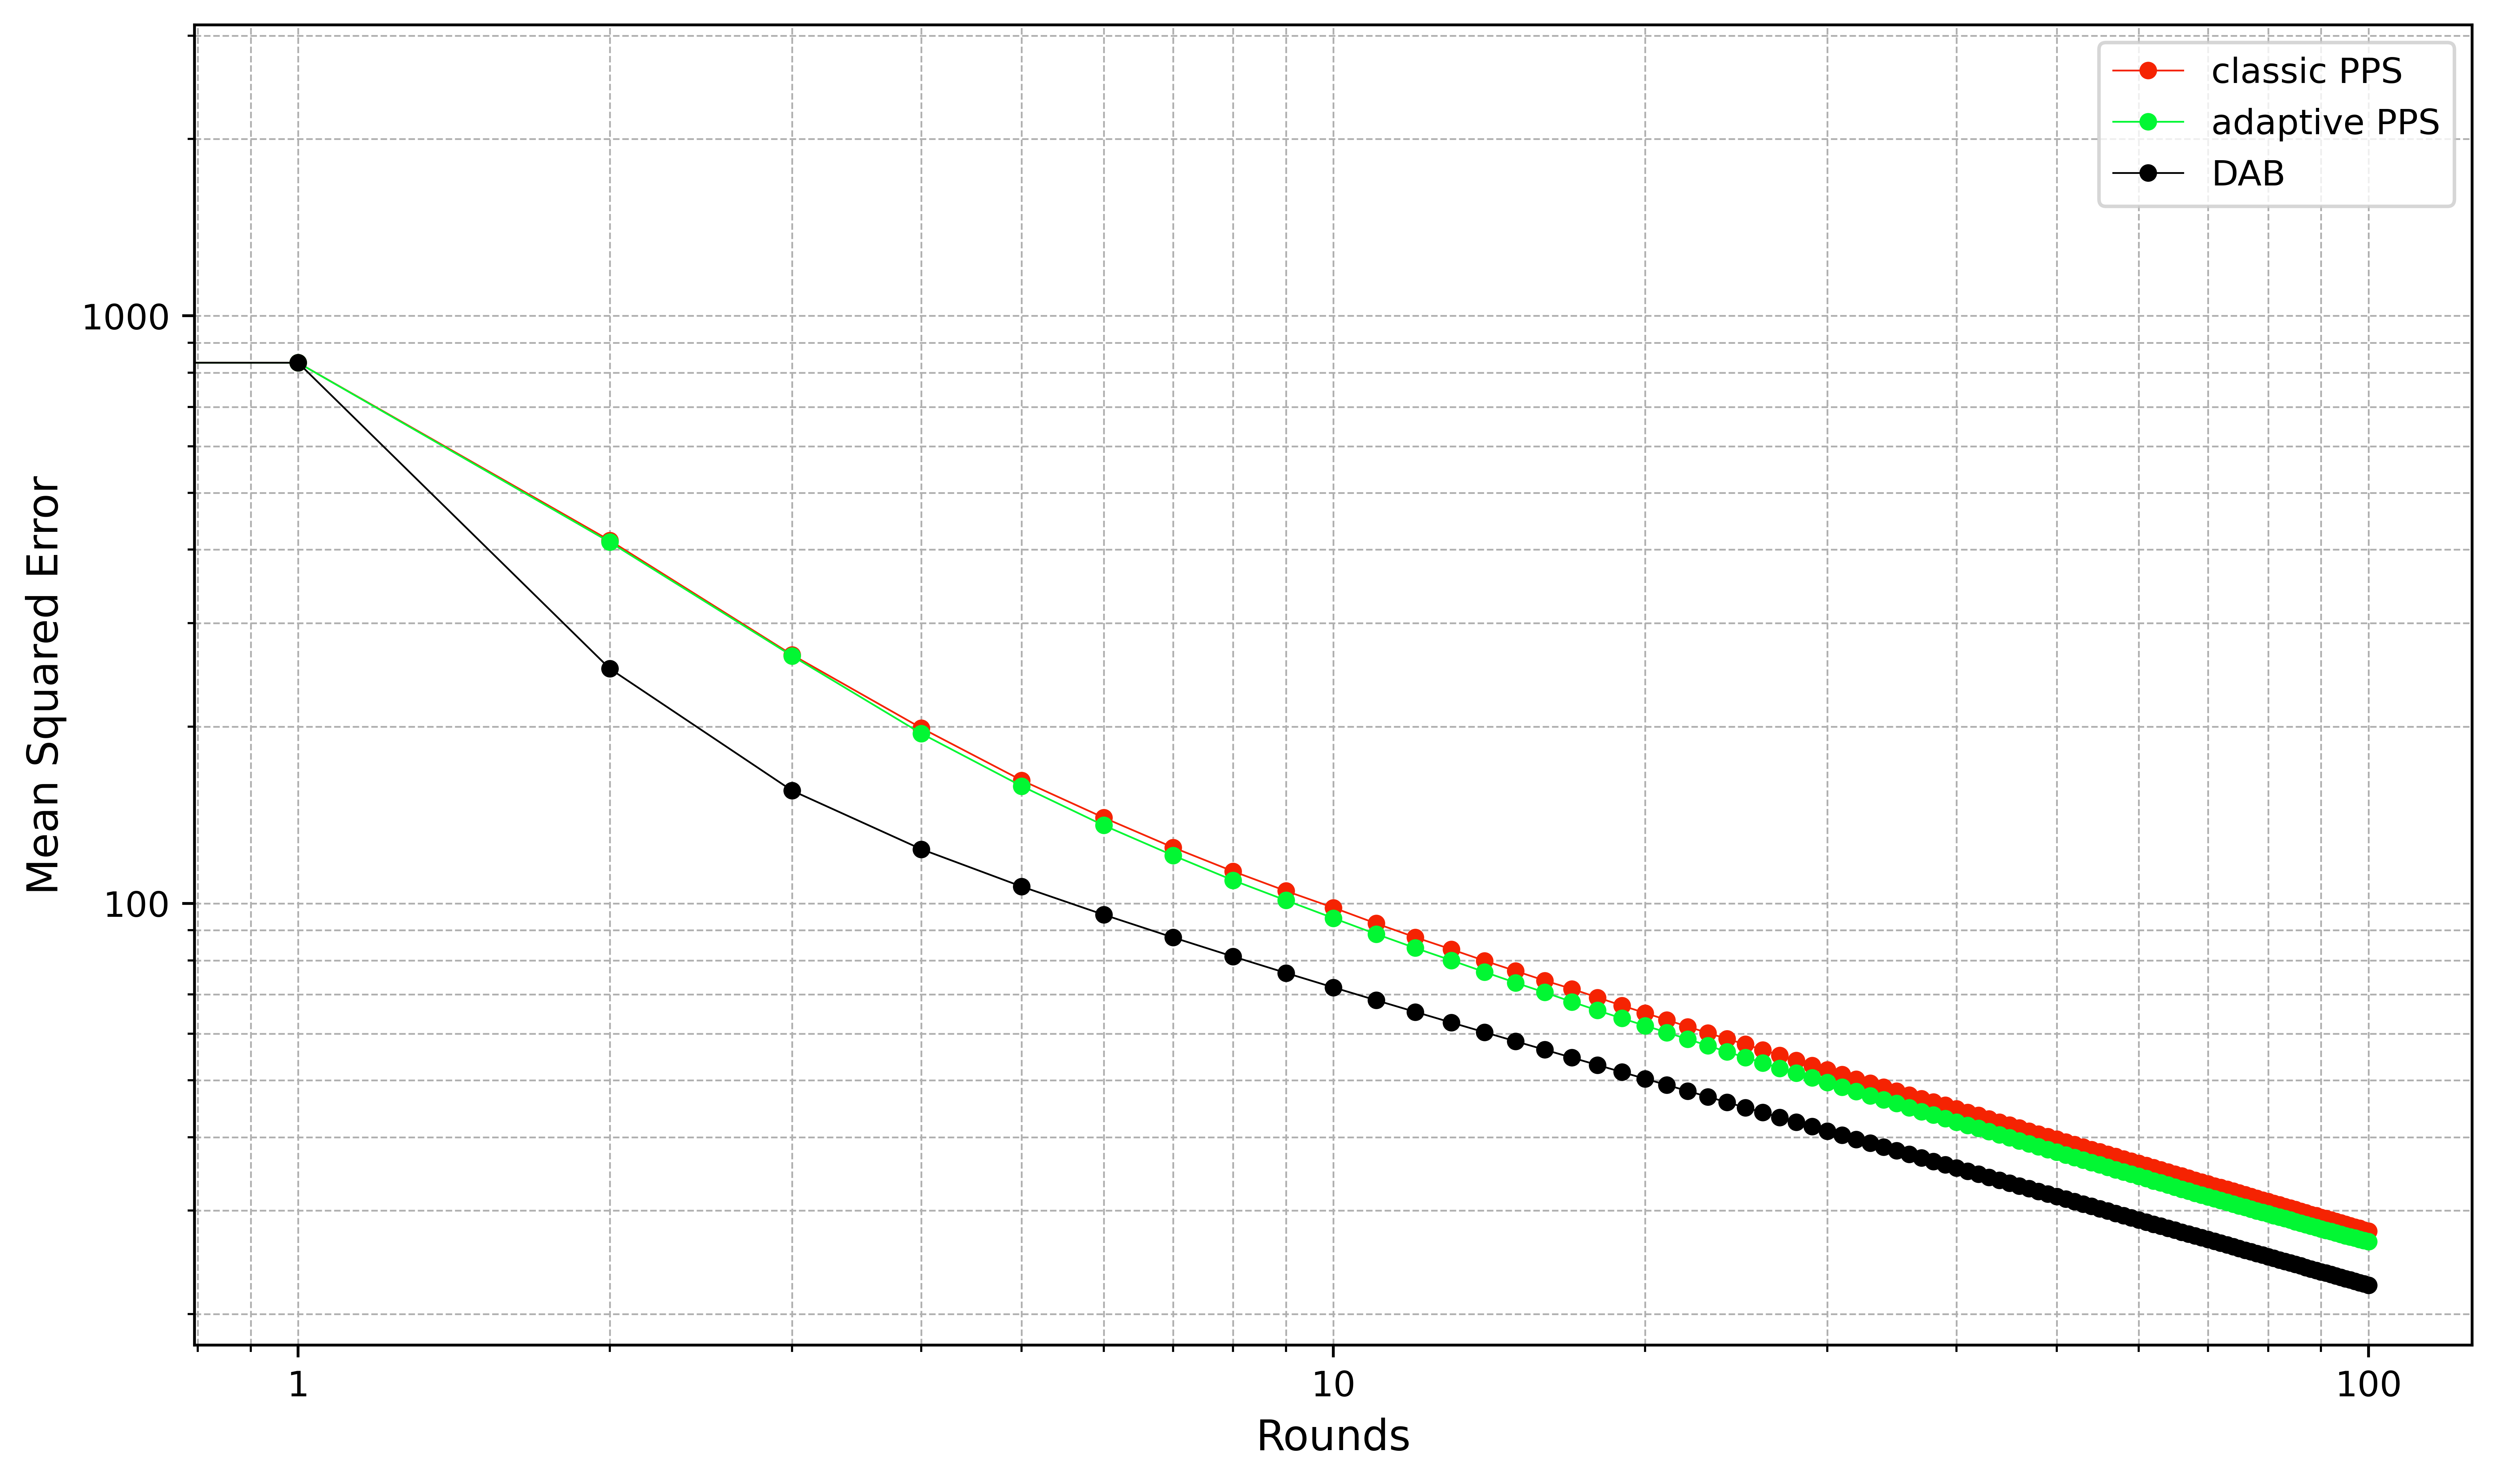
\includegraphics[width=\linewidth]{figures/Simulation_outcomes/RingGraph/DAB_vs_PPS_RG_r100_n1024_averaged_loglog.png}
    \caption{Ring graph - mean squared error per rounds - log-log}
    \label{fig:ringgraphMSEperRoundLogLog}
\end{figure}
\begin{figure}[]
    \centering
    \scalebox{0.8}{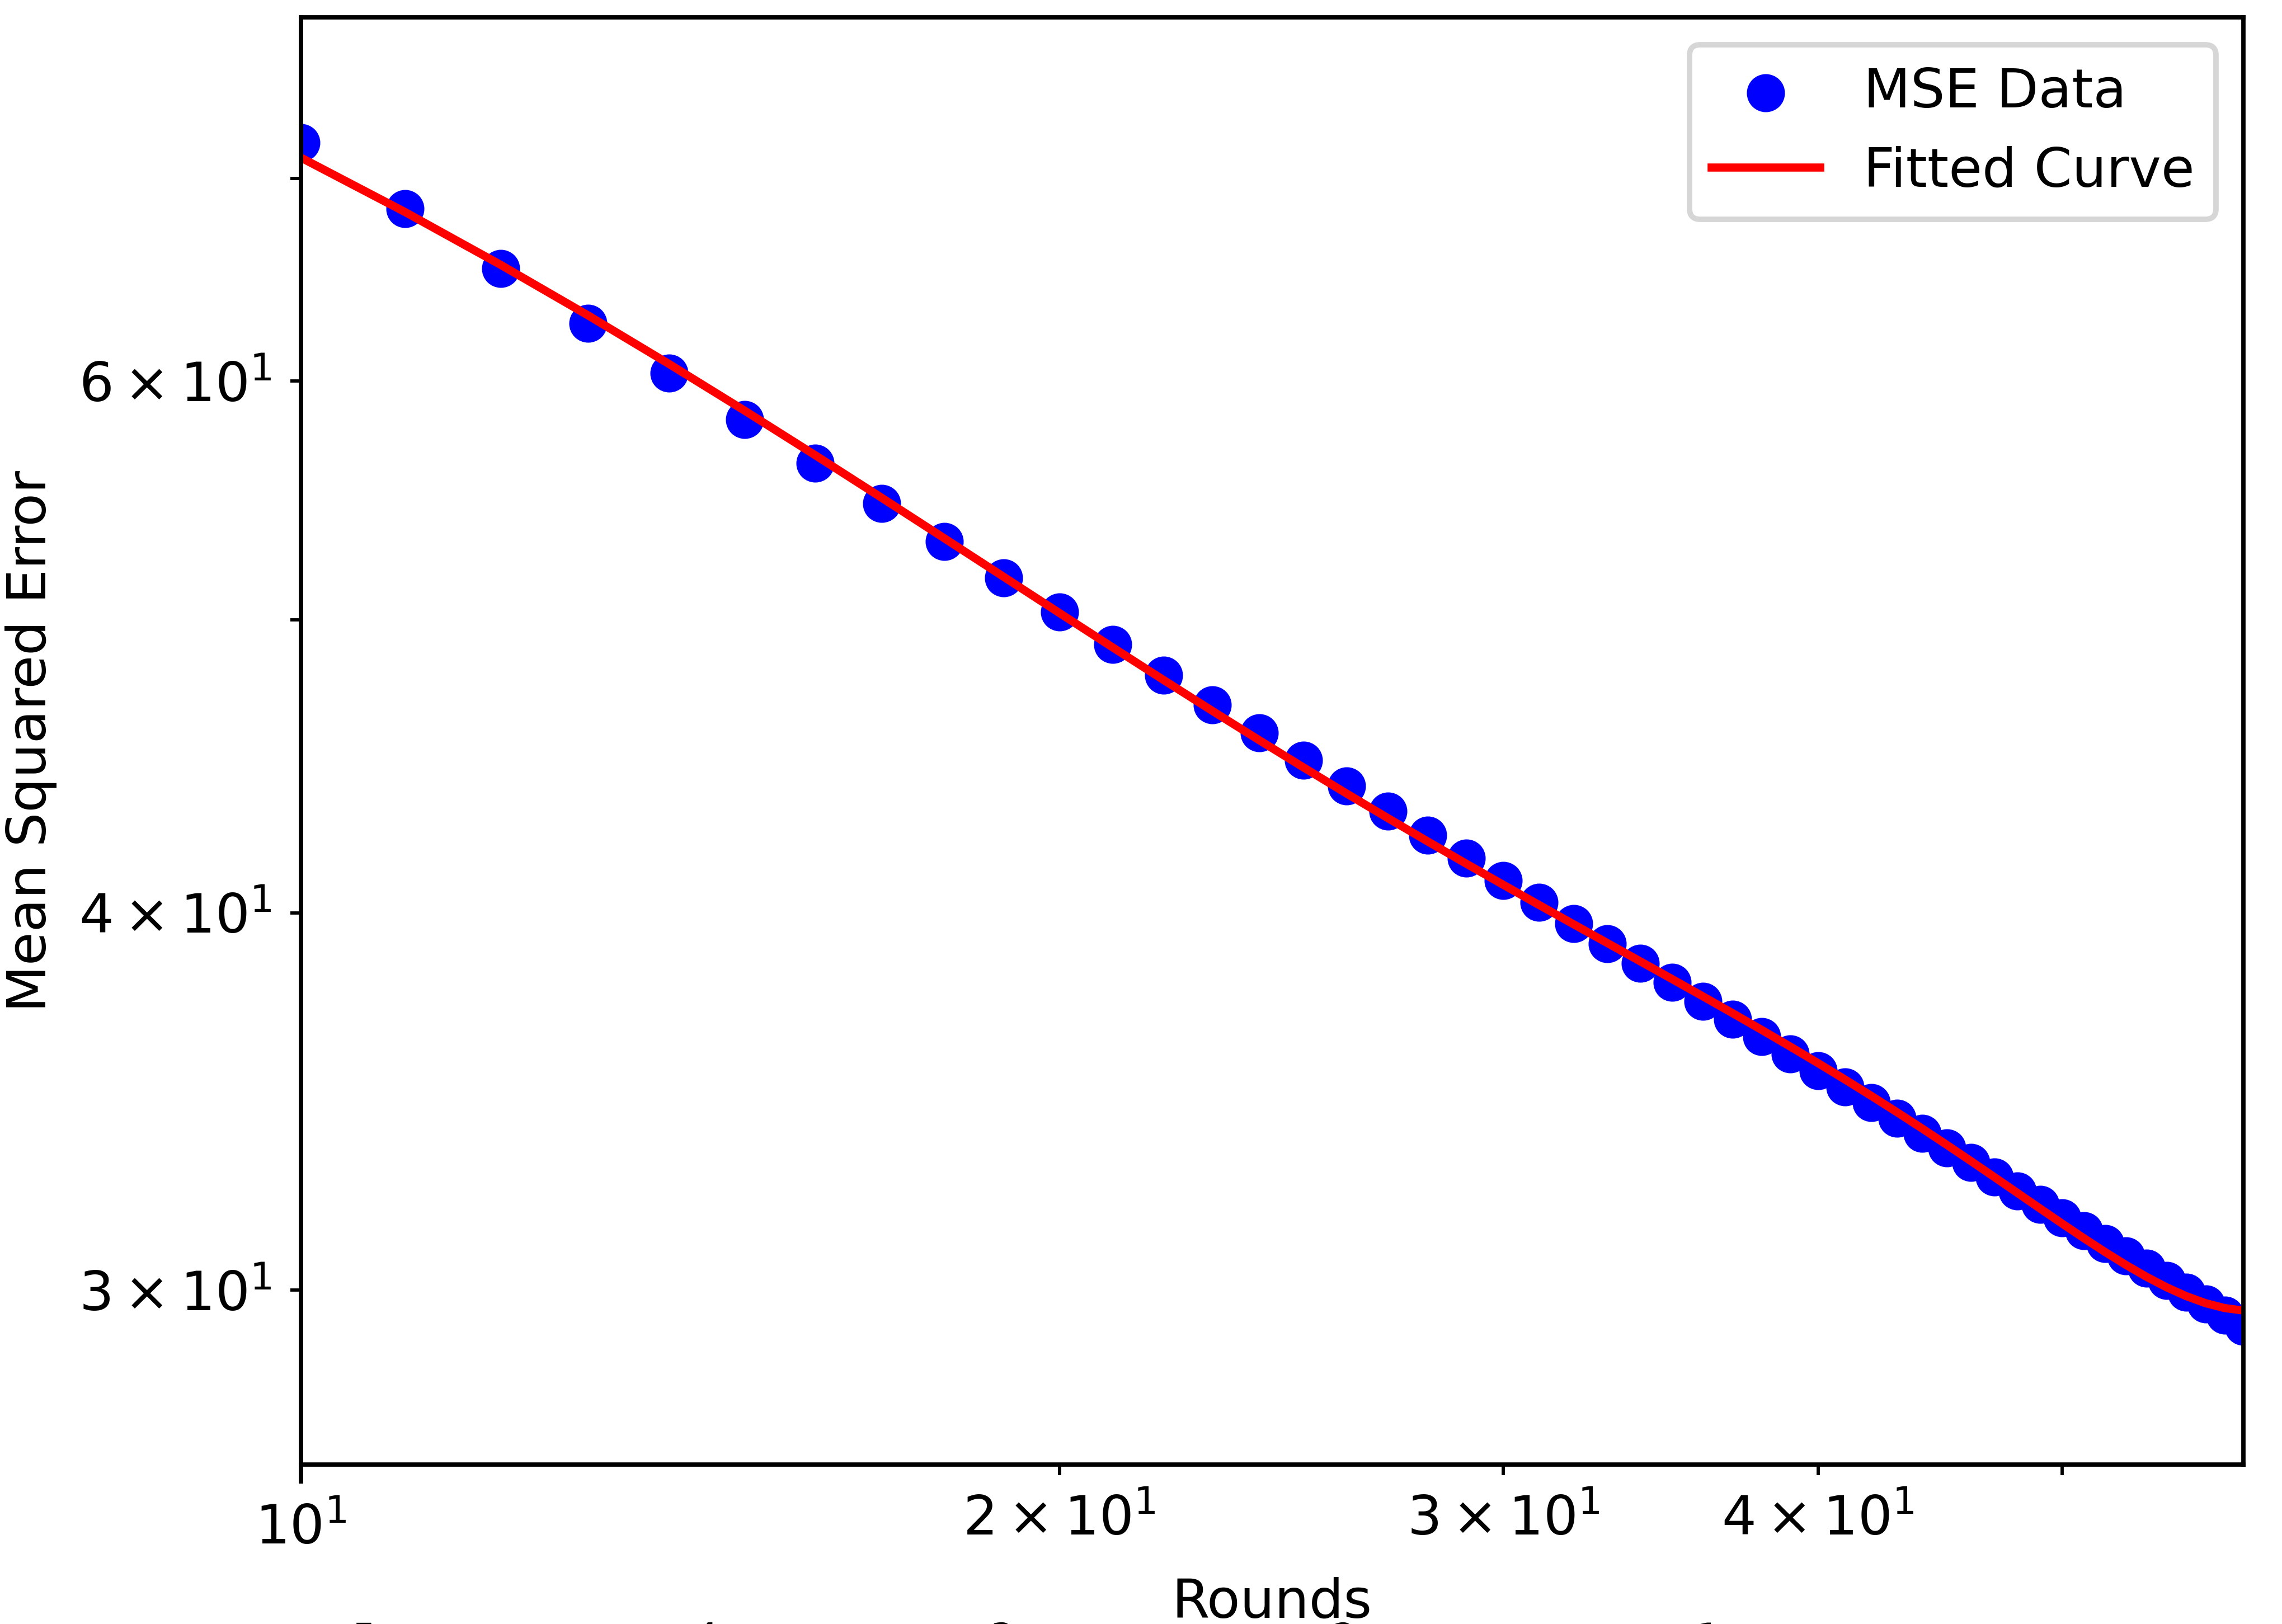
\includegraphics{figures/Simulation_outcomes/RingGraph/DAB/DAB_modelfitting_rounds_59_model_2.png}}
    \caption{Ring graph - polynomial regression fit - DAB}
    \label{fig:dabRingModelFit}
\end{figure}
\begin{figure}[]
   \centering
   \scalebox{0.8}{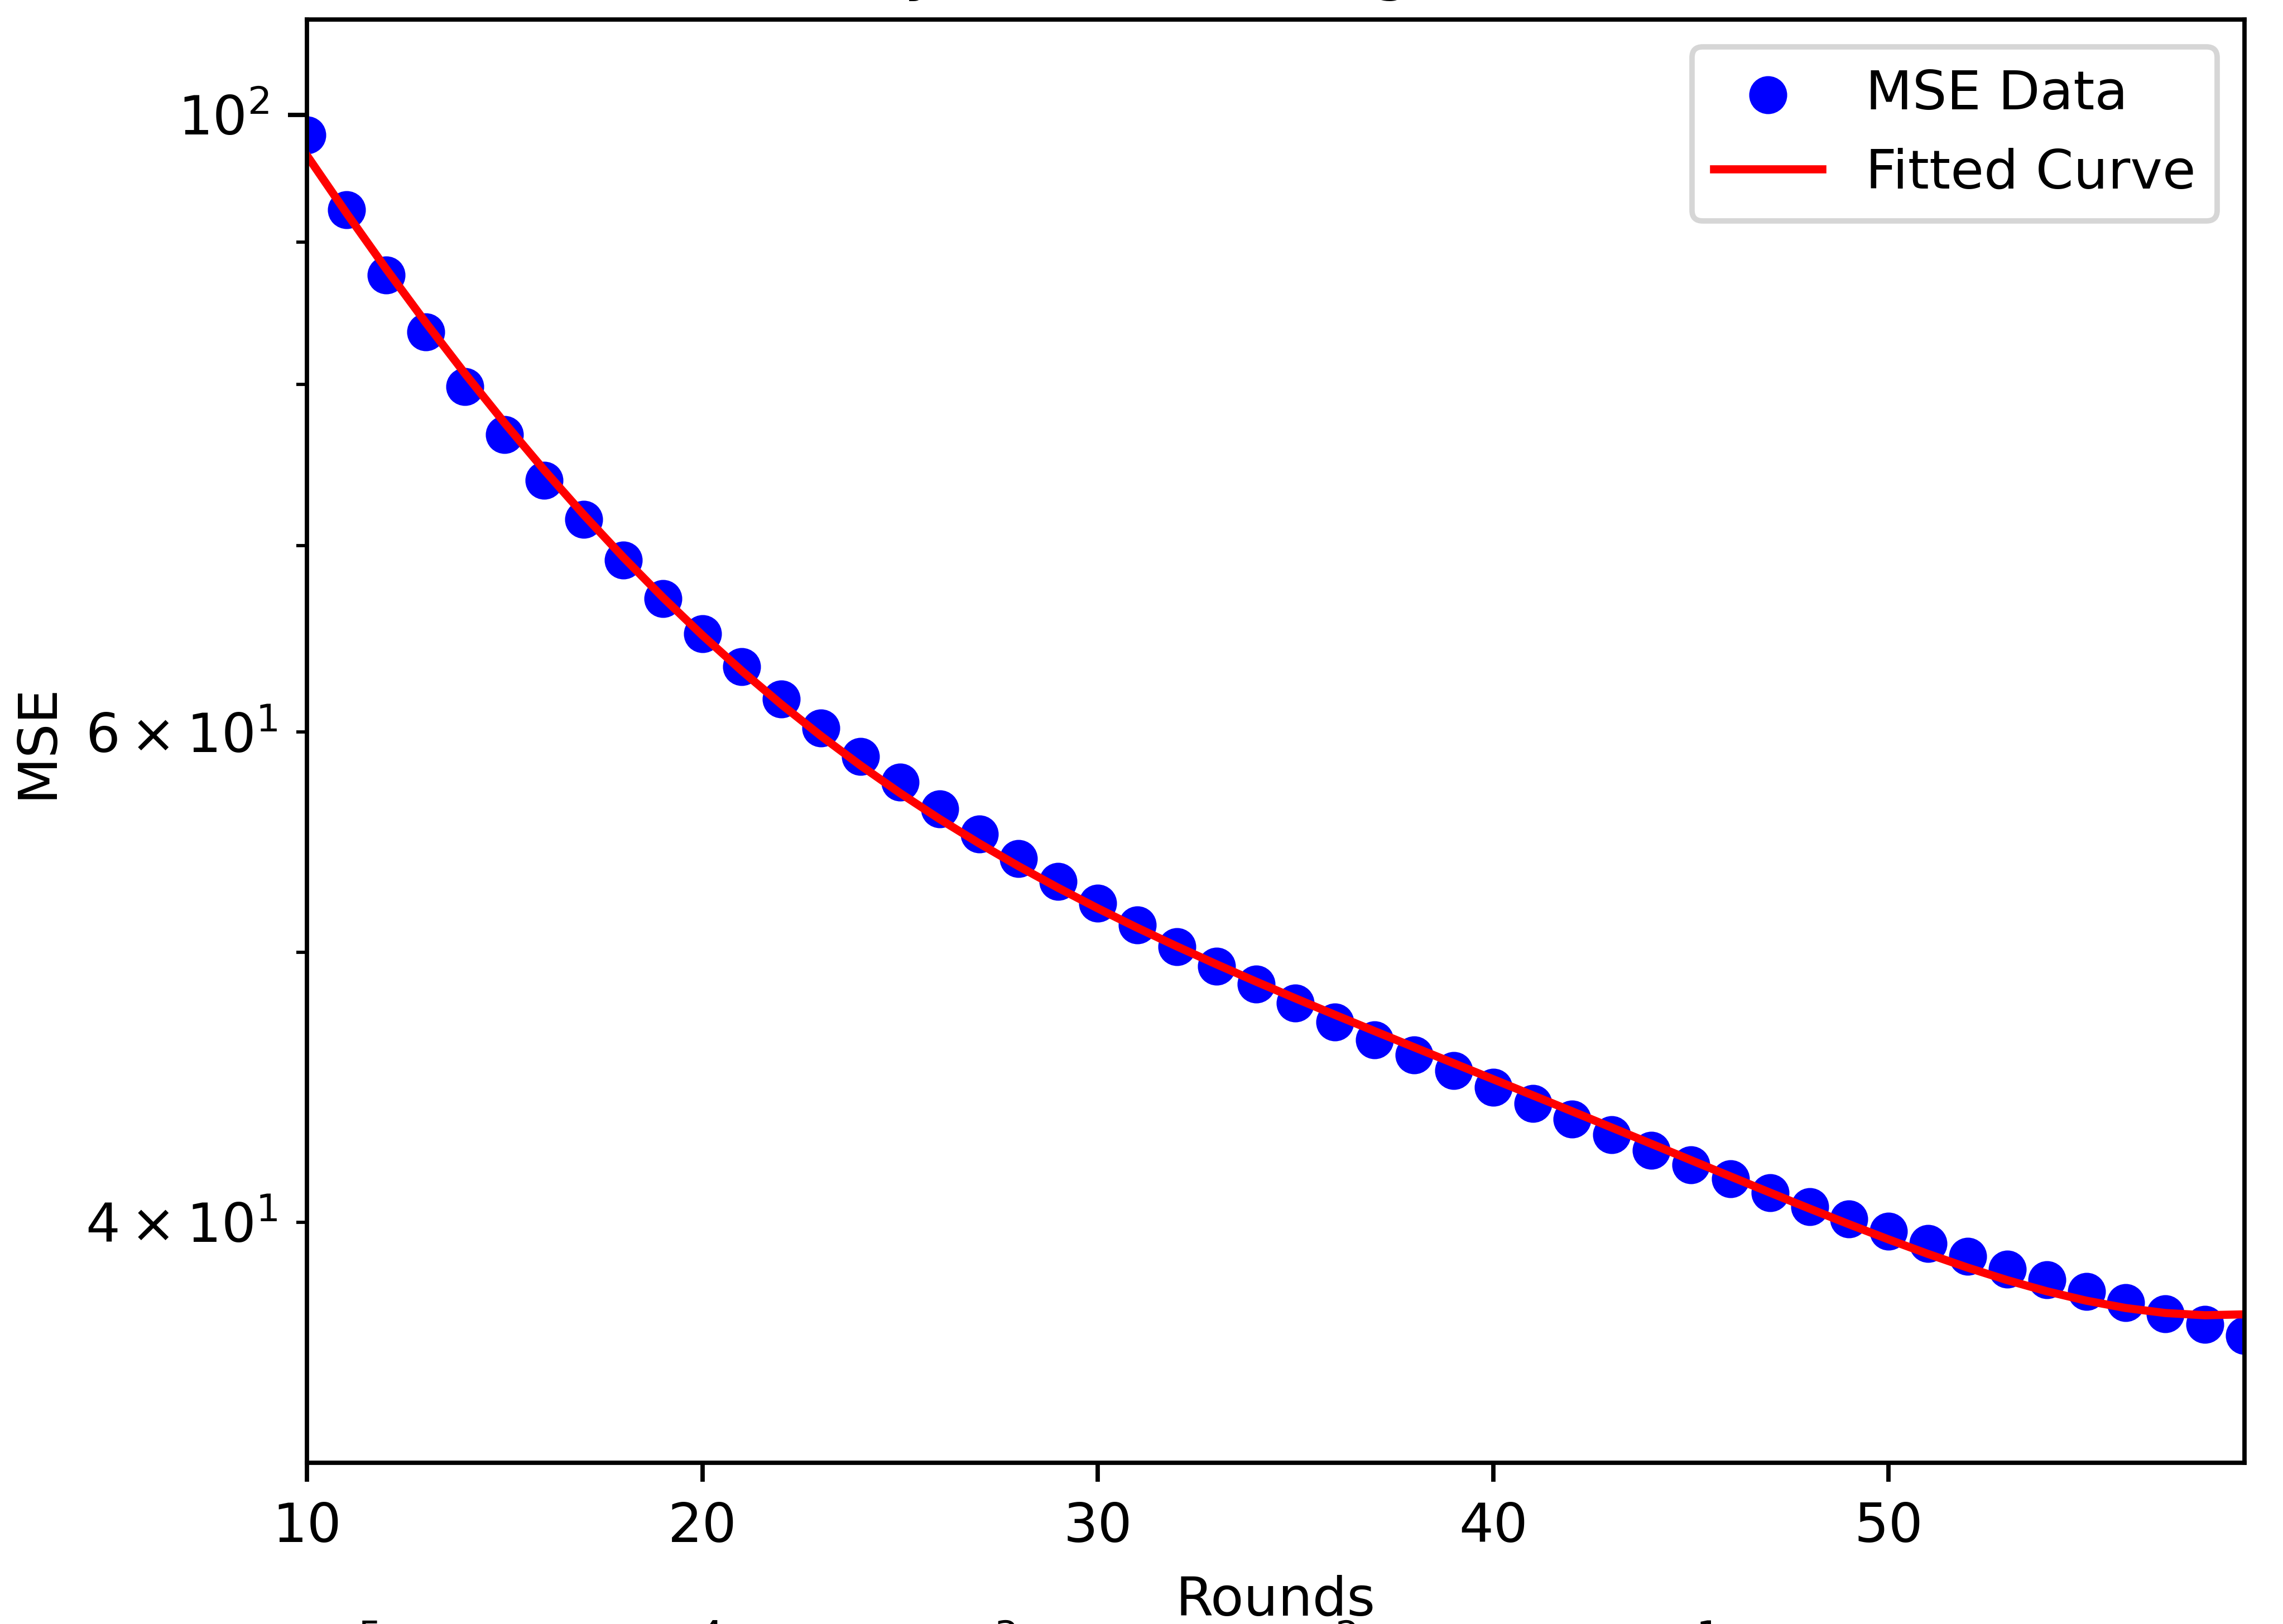
\includegraphics{figures/Simulation_outcomes/RingGraph/PPS/PPS_modelfitting_rounds_59_model_2.png}}
   \caption{Ring graph - polynomial regression fit - PPS}
   \label{fig:ppsRingModelFit}
\end{figure}
\begin{figure}[]
    \centering
    \scalebox{0.8}{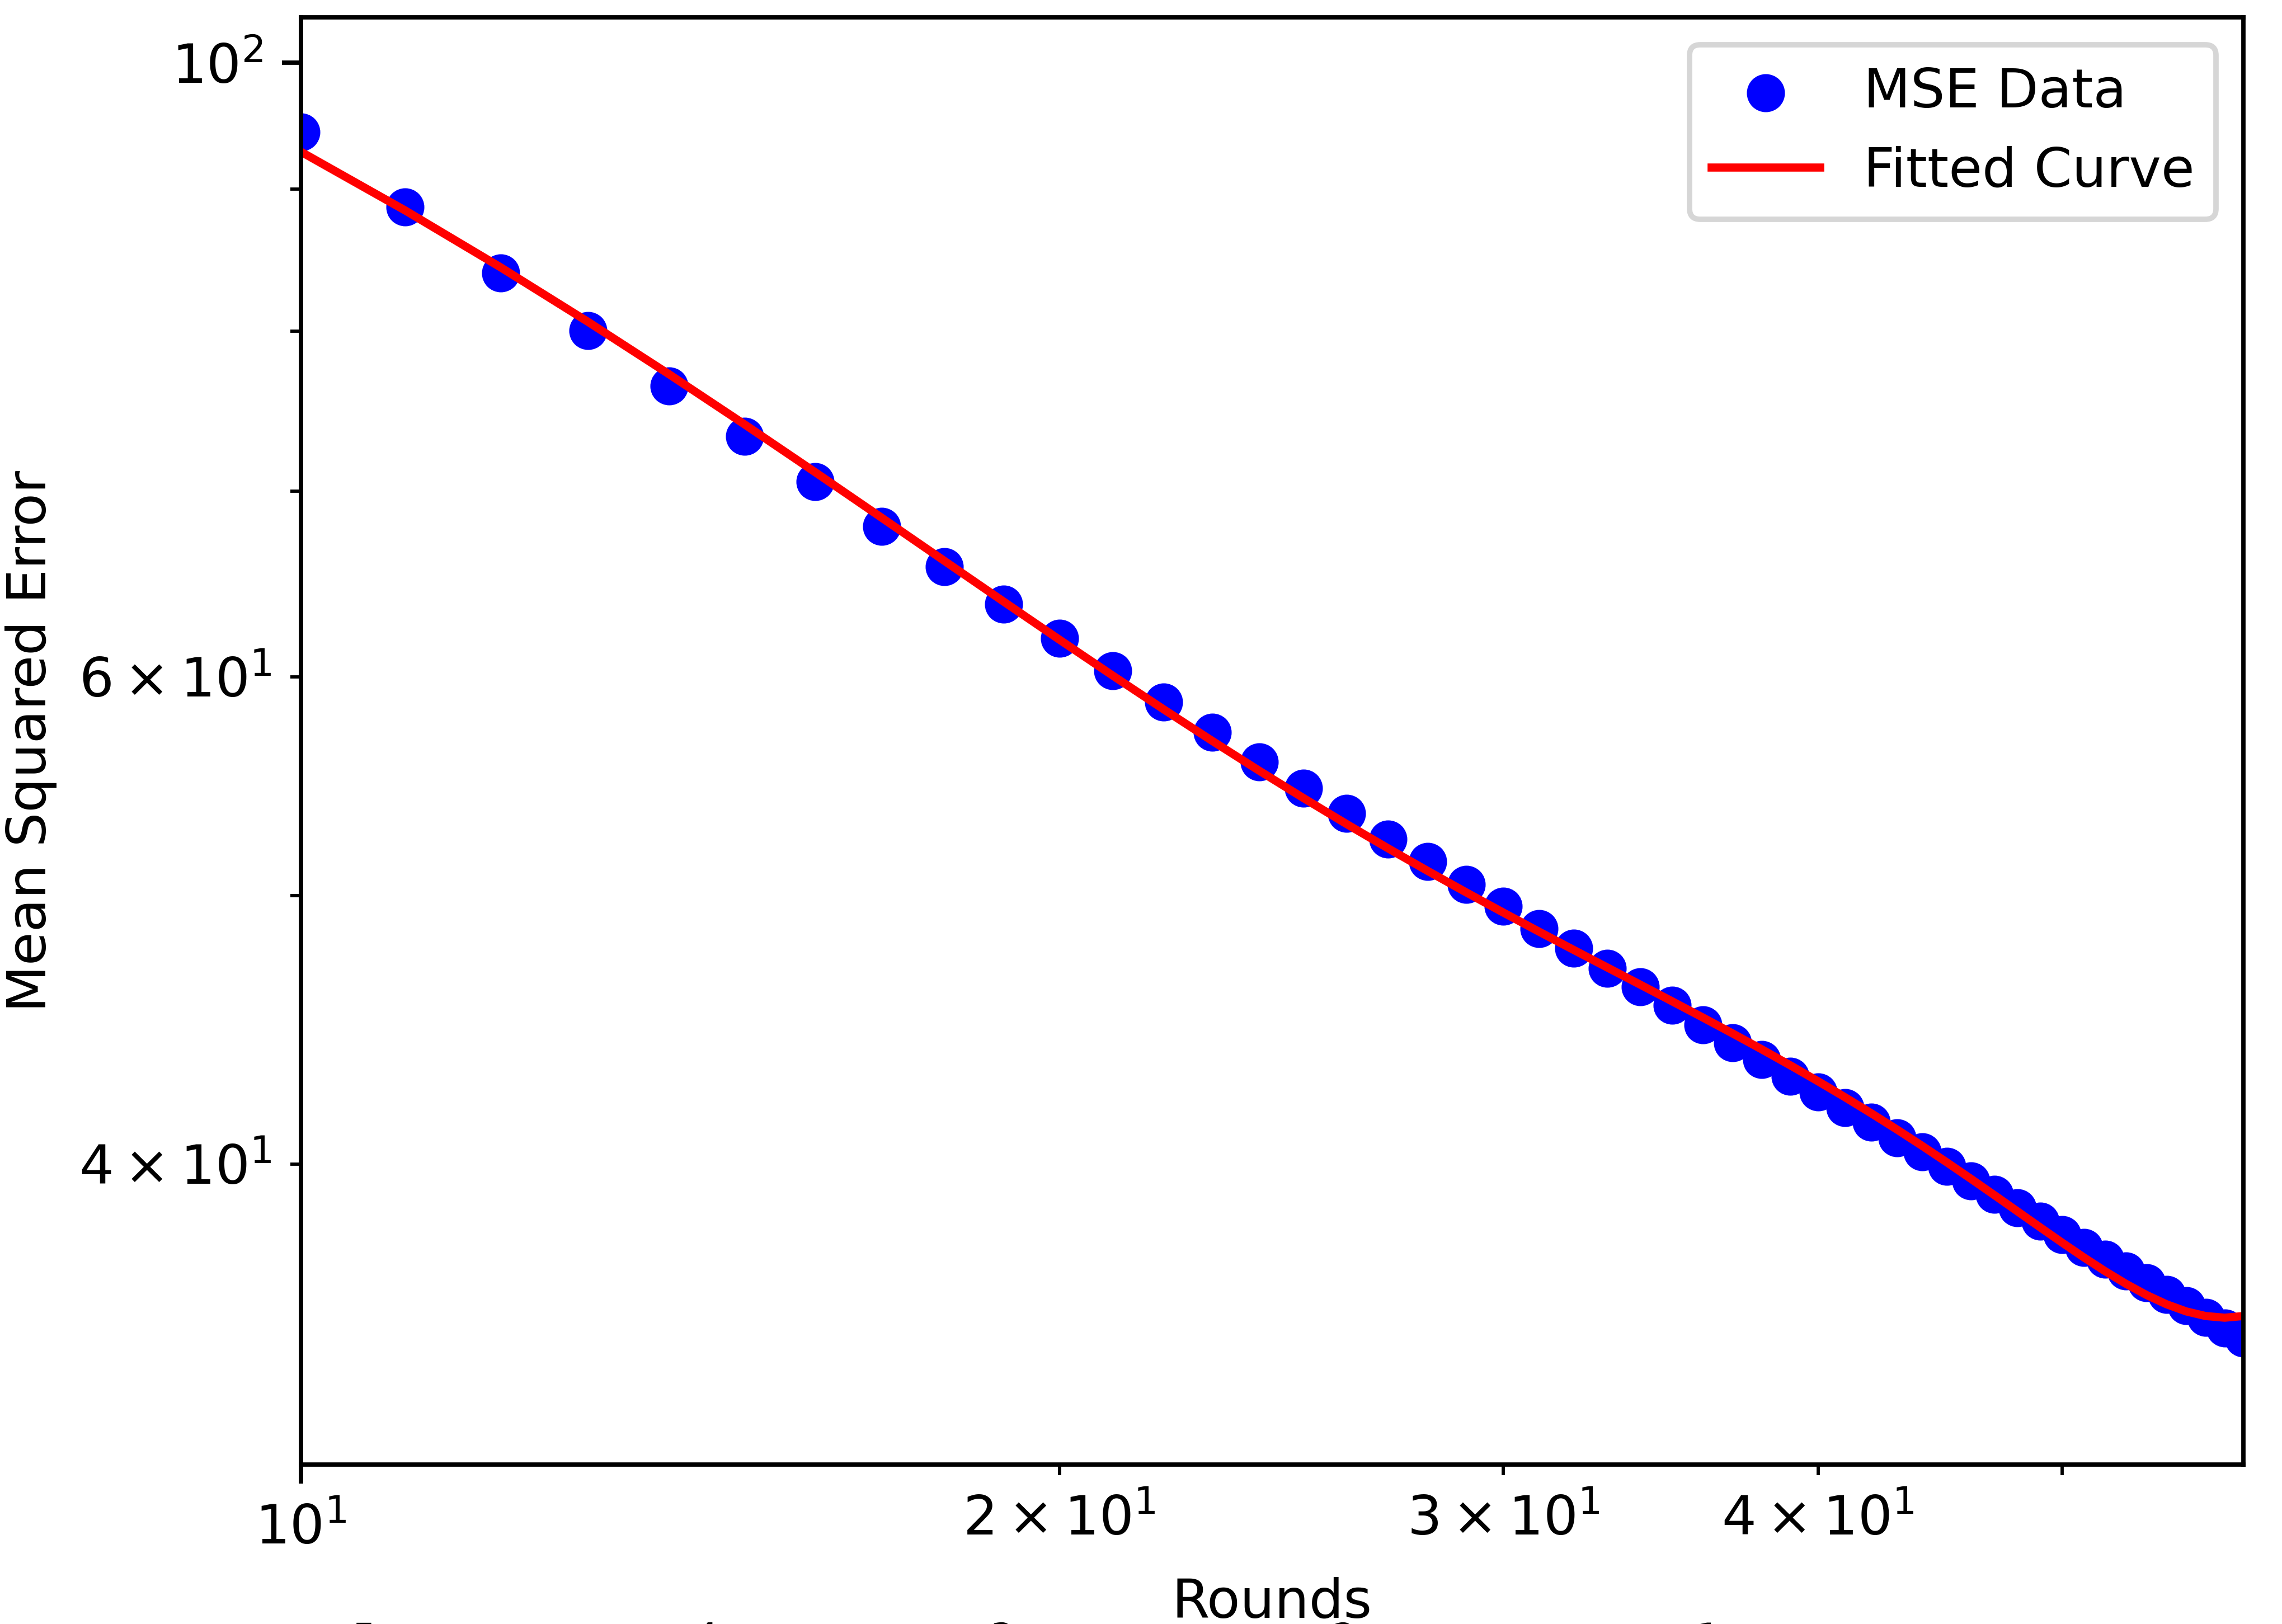
\includegraphics{figures/Simulation_outcomes/RingGraph/ATPPS/ATPPS_modelfitting_rounds_59_model_2.png}}
    \caption{Ring graph - polynomial regression fit - ATPPS}
    \label{fig:atppsRingModelFit}
\end{figure}
\begin{figure}
    \centering
    \scalebox{0.8}{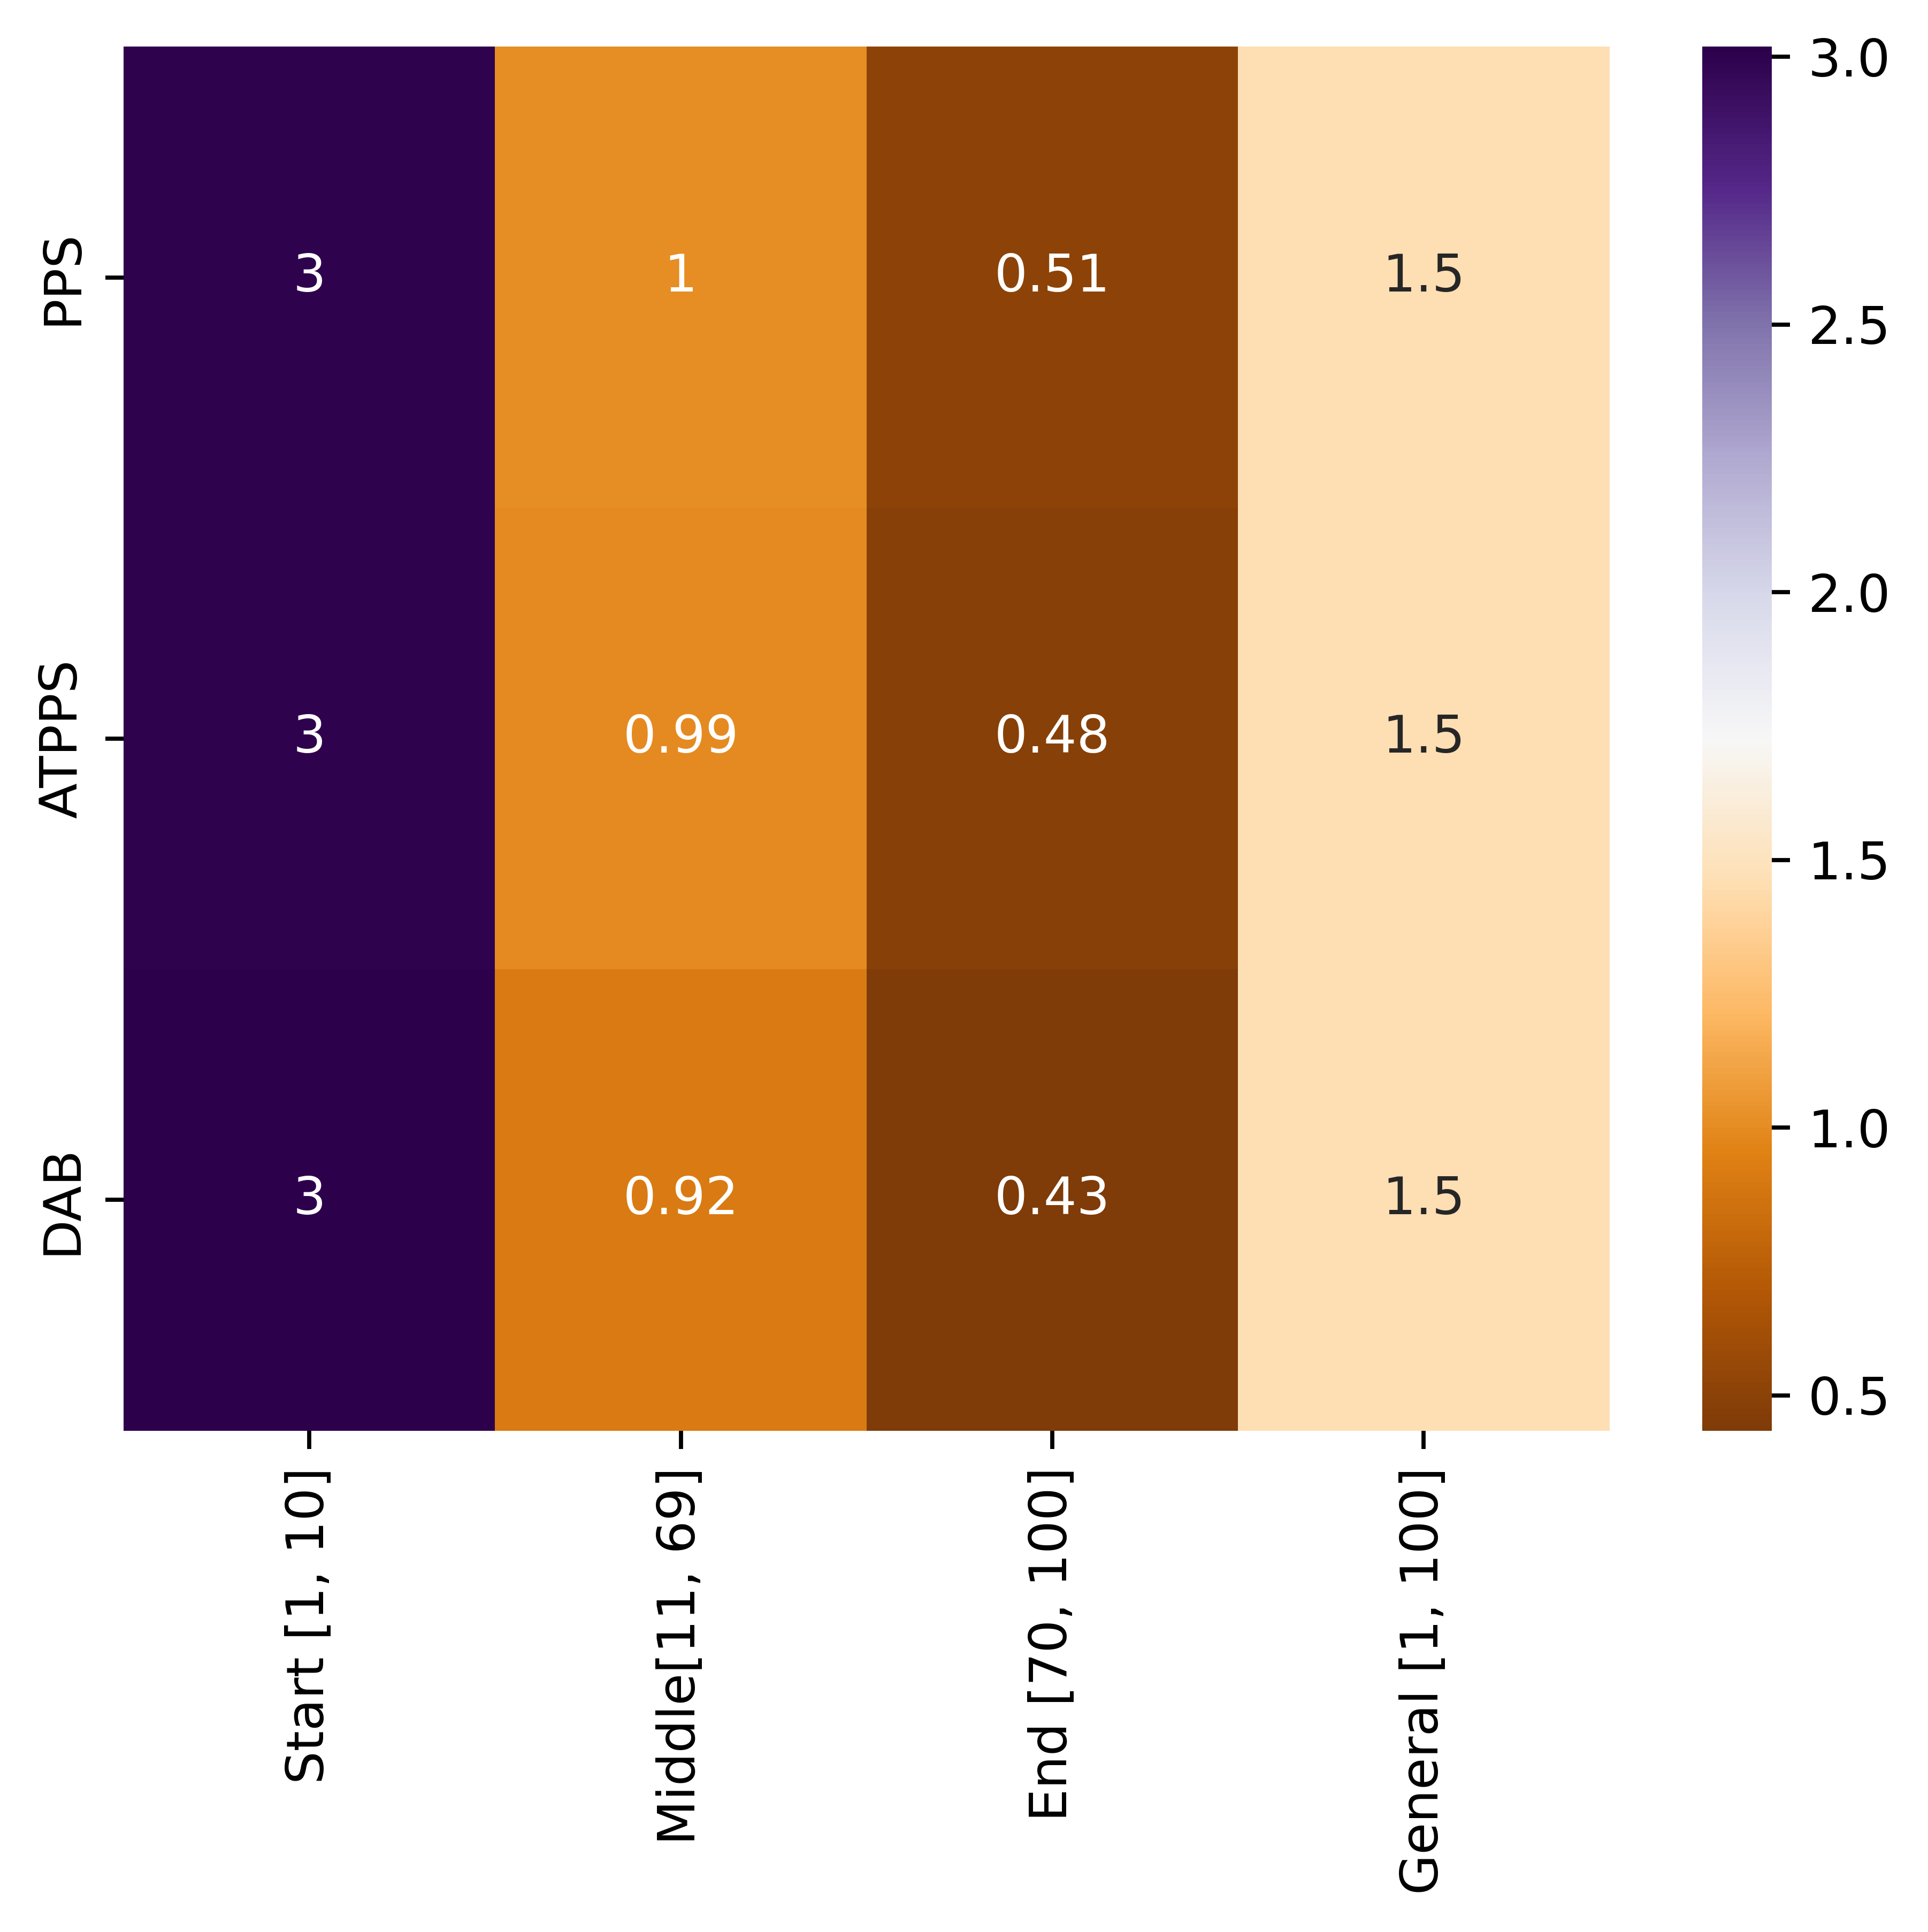
\includegraphics{figures/Simulation_outcomes/RingGraph/DAB_vs_PPS_vs_ATPPS_slopesheatmap_100rounds_log_log.png}}
    \caption{Ring graph - heat map of slopes per region - log-log}
    \label{fig:ringgraphslopes}
\end{figure}

\section{Torus Grid Graph}\label{sec:torusgridGraph}
Figure \ref{fig:torusMSEperRoundLogLog} shows the MSE reduction over rounds on a Torus Grid graph, plotted on a log-log scale. The DAB curve has a slightly faster initial reduction compared to PPS' and ATPPS' curves in the beginning (rounds 1 to 7). The slope in this region is superior for the DAB with a value of -2.1 compared to approximately -1.5 for the Push-Pull Sum-based algorithms (figure \ref{fig:torusgraphslopes} - log-log). The PPS and ATPPS curves maintain nearly identical performances during the middle region (rounds 8 to 40), reducing MSE at a similar rate, with a slope of -1.2 for the PPS curve and -1.3 for the ATPPS curve. DAB shows a similar slope as the PPS. In the final region DAB scores the highest slope with a value of -2, followed by the ATPPS with a value of -1.7. The PPS achieves a slope of -1.4 in this region. This suggests that DAB and ATPPS adapt more efficiently to the graph's structure during advanced rounds. PPS and ATPPS exhibit convergence, but they lag behind the DAB in reaching such low MSE values. Tori have more structured connectivity compared to a Star or Complete graph, allowing better distribution of loads via deterministic interactions. DAB's superior performance stems from it leveraging this regularity. The ATPPS achieves a balanced trade-off in this scenario. It outperforms the PPS approach, particularly in later rounds, where its adaptive mechanism prevents redundant load transfers and prioritizes exchanges that have a more significant impact on error reduction.

The uniform neighborhood structure of Tori ensures that DAB's deterministic decisions (e.g., always choosing the minimal neighbor) are consistently effective across the graph. The algorithm does not suffer from suboptimal decisions introduced by probabilistic neighbor choices, which makes it well-suited to the topology. Both PPS and ATPPS protocols rely on randomly selecting a neighbor for load exchange. While this randomness is beneficial in irregular or dense graphs (e.g., Star or Complete graphs), it is less effective in structured topologies compared to the DAB, like a Torus Grid. The Push-Pull Sum-based algorithms do not always target the most unbalanced areas. This means that load propagation can sometimes "stall" in certain regions, where they require more rounds to achieve global balance. The ATTPS draws its benefit over the PPS (especially in later rounds) by deciding which option of the available subset is the best. The discrepancy between the two load balancing algorithms widens in the last few rounds as trades between two nodes with higher load differences are more impactful once the network is already heavily balanced.

The fitted polynomial curve of degree 5 matches the MSE data for DAB effectively. During the rounds 10 to 39 the MSE data is fitted to the polynomial regression model following the equation: 
\begin{align}
    MSE_r=-1.35\times 10^{-6}r^{5}+ 1.89\times 10^{-4}r^{4}-0.01r^{3}+0.30r^{2}-4.6r+34.10    
\end{align}
as shown in figure \ref{fig:dabTorusModelFit} a). This suggests that in these rounds, the MSE reduction follows a complex pattern, as the loads propagate to different regions of the graph thanks to the wrap-around edges of the Tori. In later rounds, the performance of the DAB can be captured by a polynomial curve of degree 3 with the equation:
\begin{align}
    MSE_r=-6.01\times 10^{-<6}r^{3}+1.66\times 10^{-3}r^{2}-0.16r+6    
\end{align}
(figure \ref{fig:dabTorusModelFit} b)). At this stage, load balancing stabilizes, and the reduction in MSE becomes more linear or gradual. Thus, a lower-degree polynomial suffices to model the behavior in these later rounds. The curve behavior for the PPS and ATPPS are similar to that of the DAB curve expressed for rounds 10 to 39 by the equations:
\begin{align}
    MSE_r=-5.54\times 10^{-6}r^{5}+7.65\times 10^{-4}r^{4}-0.04r^{3}+1.16r^{2}-16.81r+112.86    
\end{align}
for the PPS (figure \ref{fig:ppsTorusModelFit} a)) and:
\begin{align}
    MSE_r = -3.65 \times 10^{-6}r^{5} + 5.16 \times 10^{-4}r^{4} - 0.03r^{3} + 0.83r^{2} - 12.52r + 88.16    
\end{align}
for the ATPPS (figure \ref{fig:atppstorusModelFit} a)). The equations that describe the behavior of the two Push-Pull Sum-based algorithms are fitted for rounds 40 to 100 for the PPS: 
\begin{align}
    MSE_r = -1.15 \times 10^{-5}r^{3} + 3.205\times 10^{-3}r^{2} - 0.33r + 13.72    
\end{align}
(figure \ref{fig:ppsTorusModelFit} b)) and for the ATPPS is:
\begin{align}
    MSE_r = -9.99 \times 10^{-6}r^{3} + 2.80\times 10^{-3}r^{2} - 0.28r + 11.29    
\end{align}
(figure \ref{fig:atppstorusModelFit} b)).

\begin{figure}[]
    \centering
    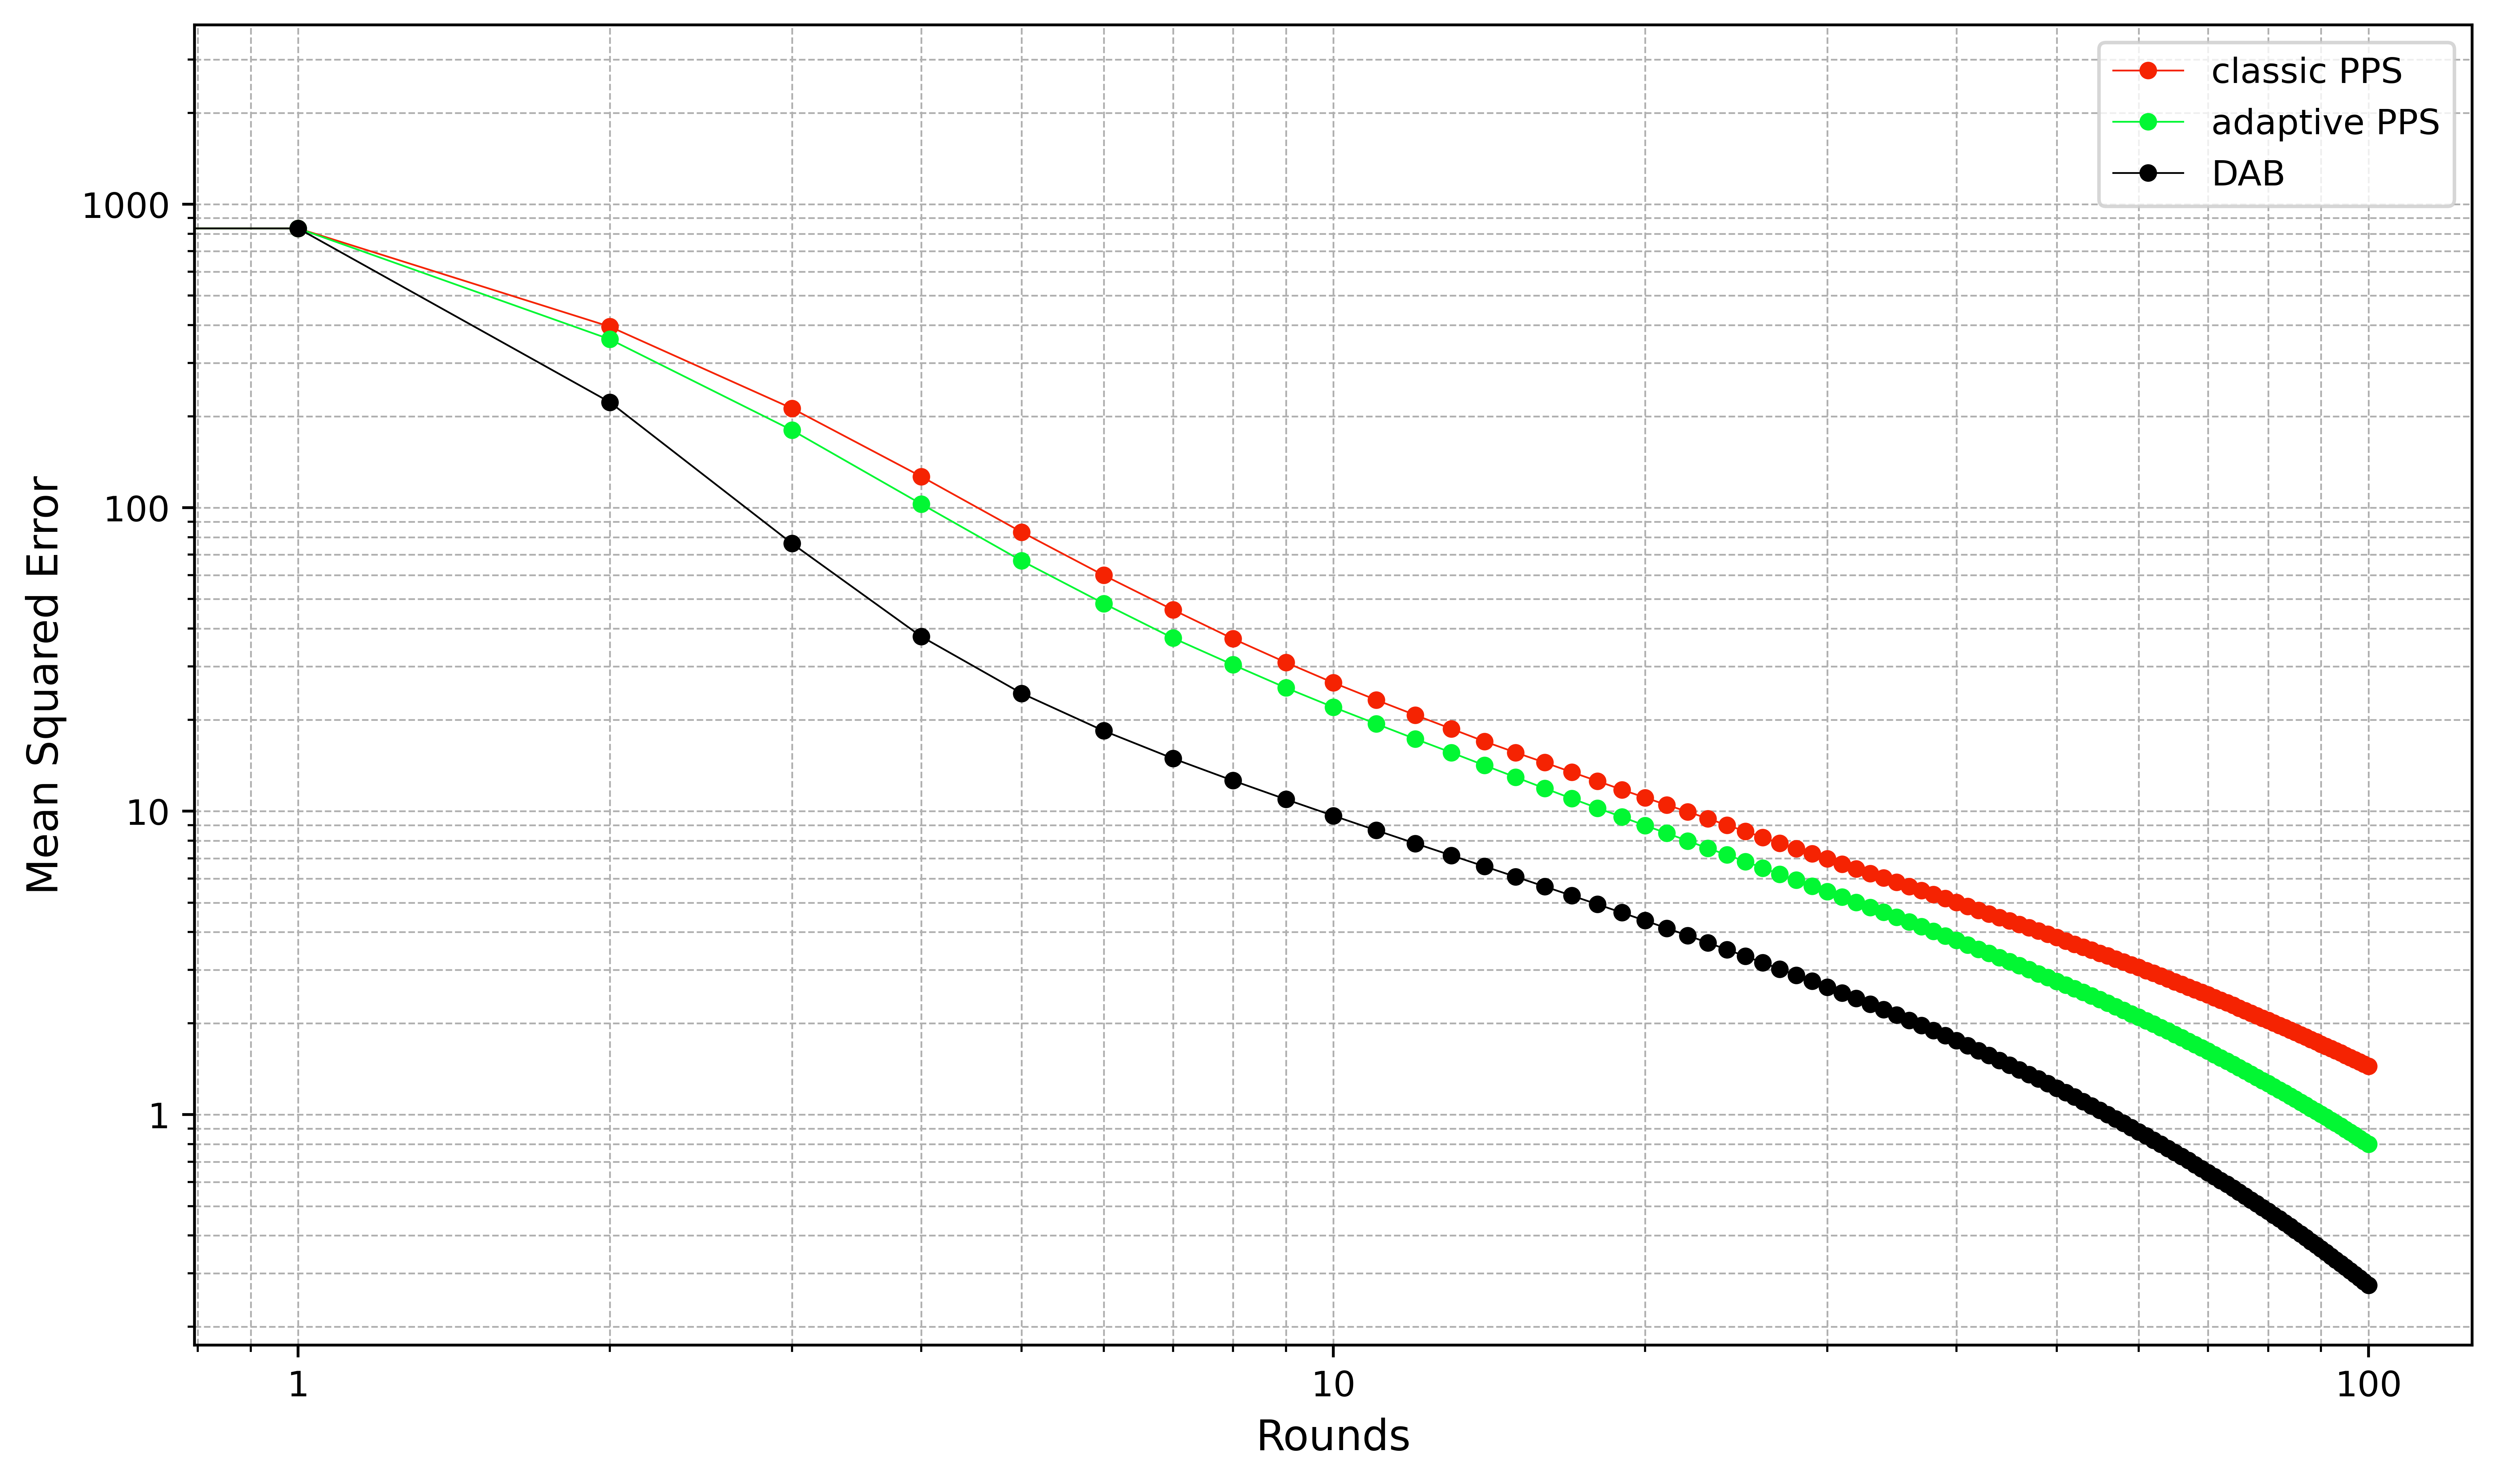
\includegraphics[width=\linewidth]{figures/Simulation_outcomes/TorusGridGraph/DAB_vs_PPS_TGG_r100_n1024_averaged_loglog.png}
    \caption{Torus Grid - mean squared error per rounds - log-log}
    \label{fig:torusMSEperRoundLogLog}
\end{figure}
\begin{figure}[!ht]
     \centering
         \subfloat[]{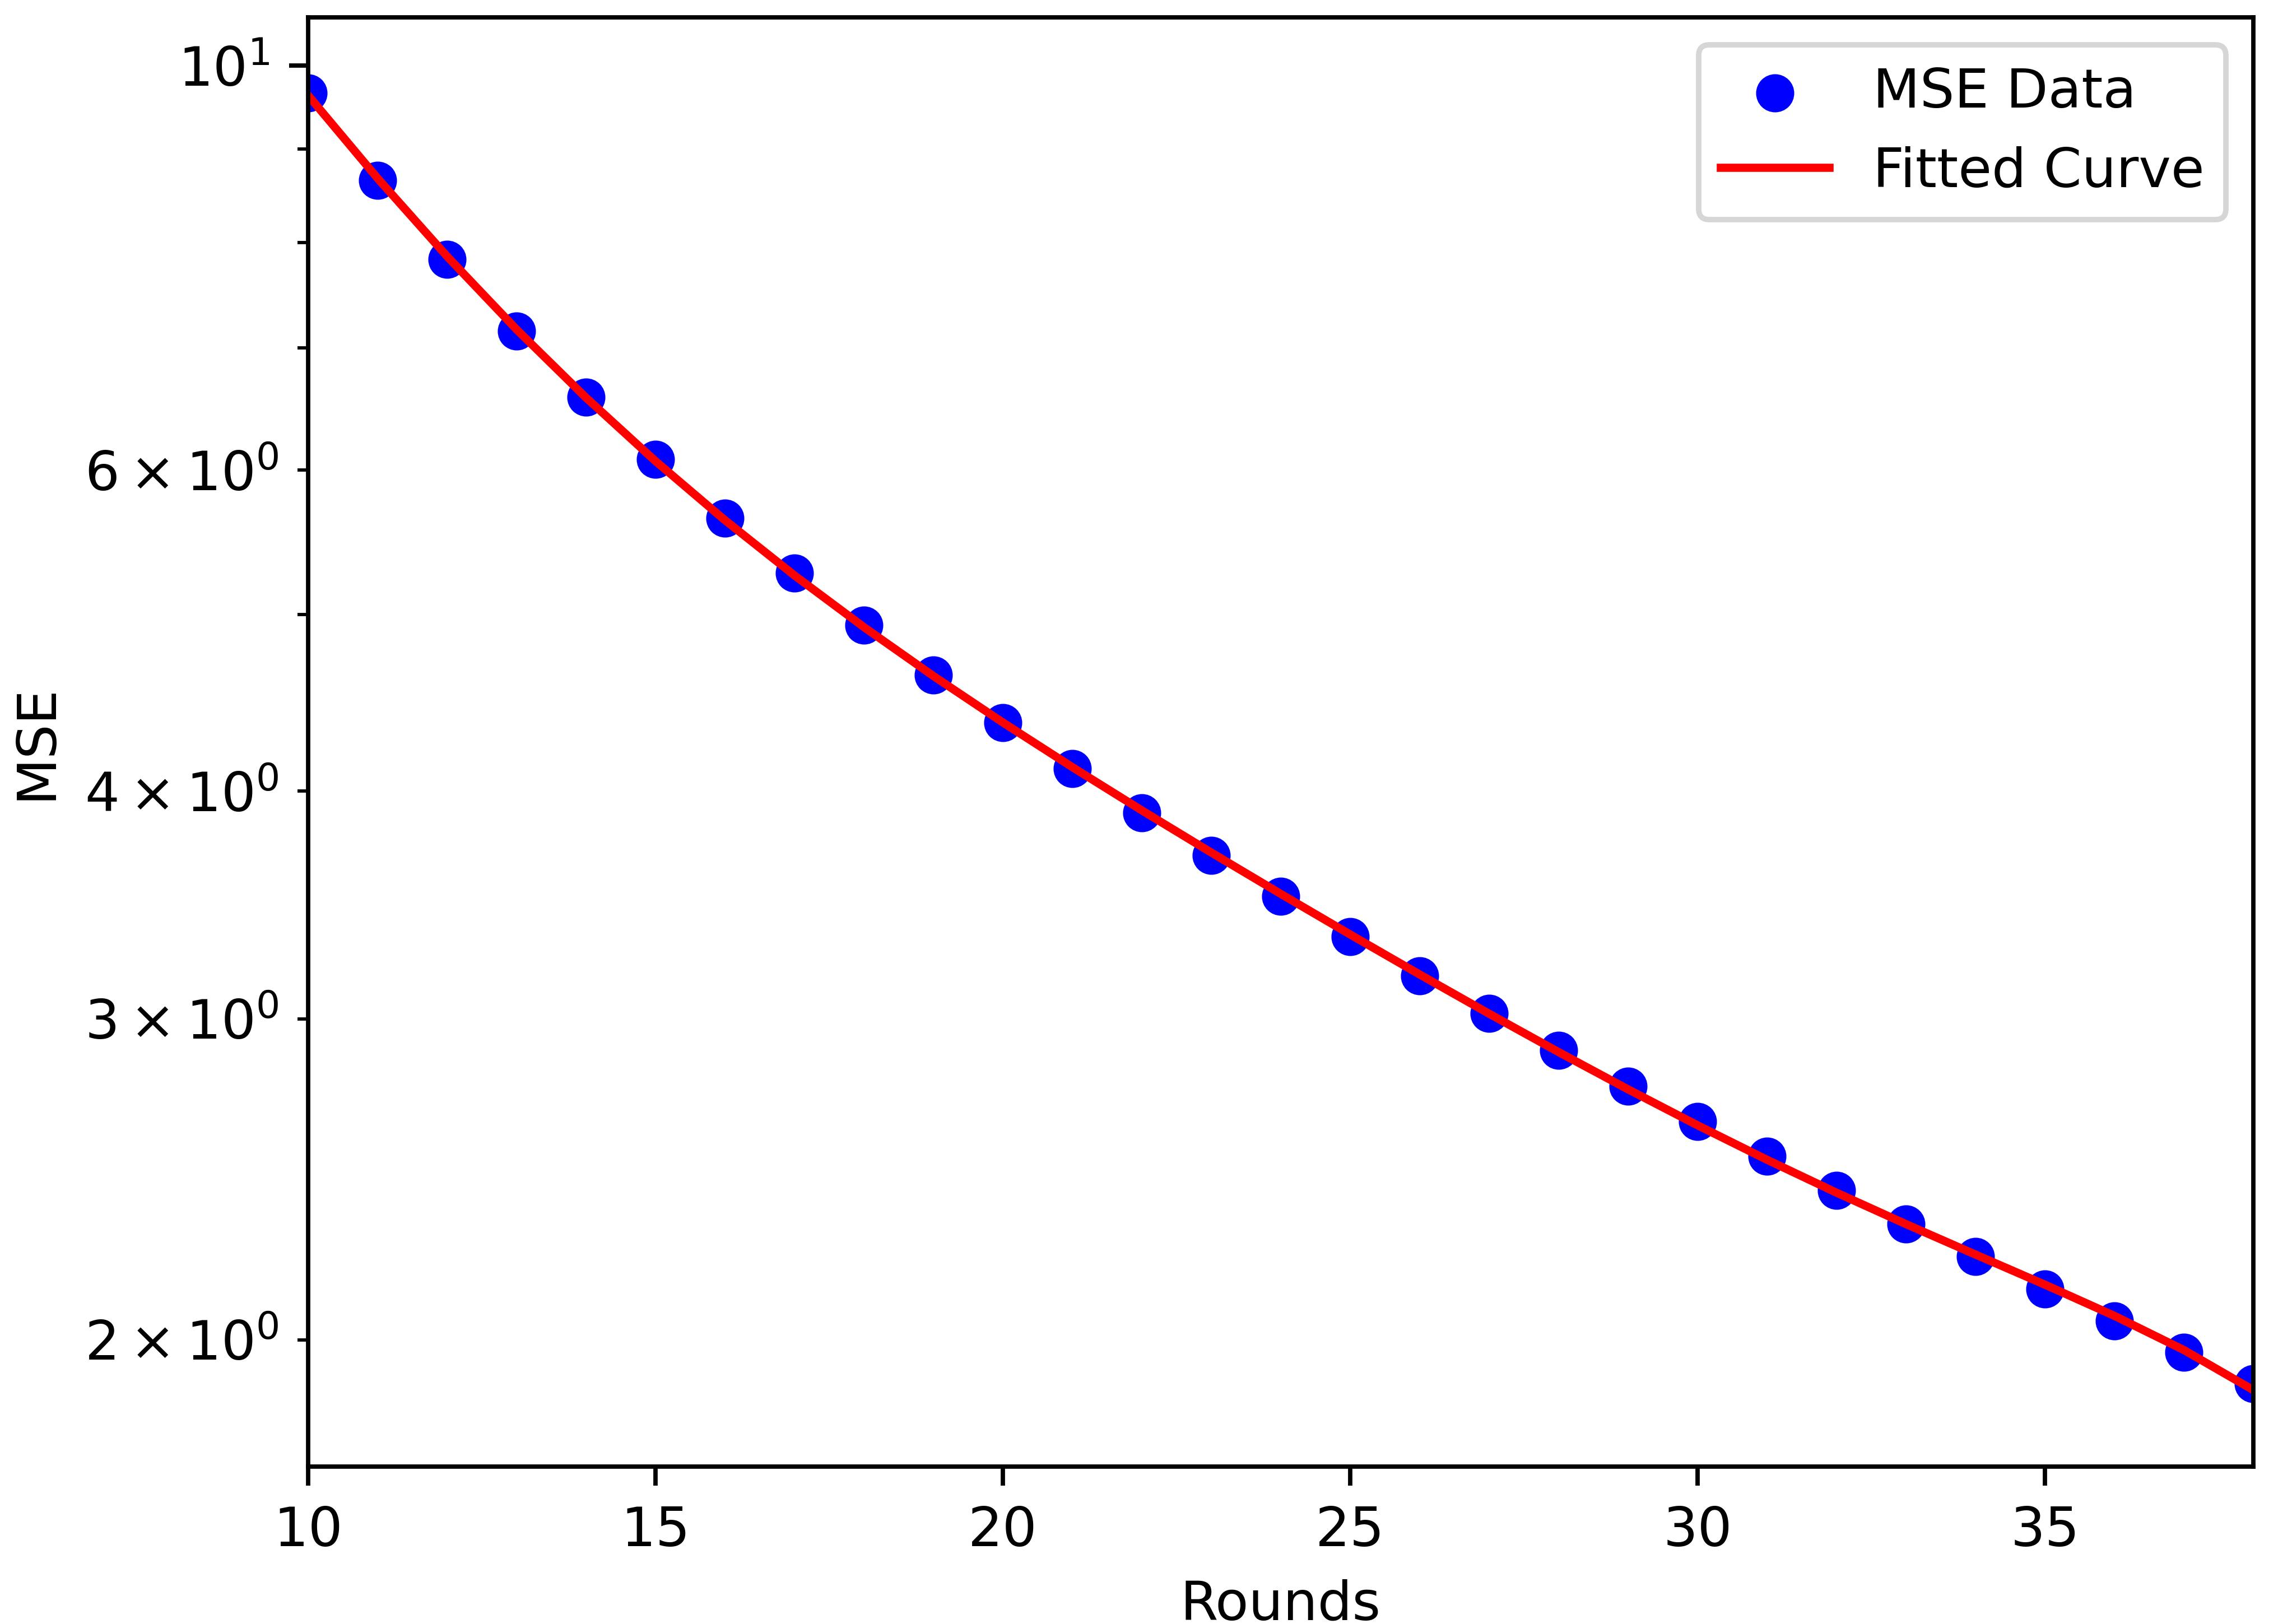
\includegraphics[width=0.49\linewidth]{figures/Simulation_outcomes/TorusGridGraph/DAB/DAB_modelfitting_rounds_38_model_2.png}}
     \hfil
         \subfloat[]{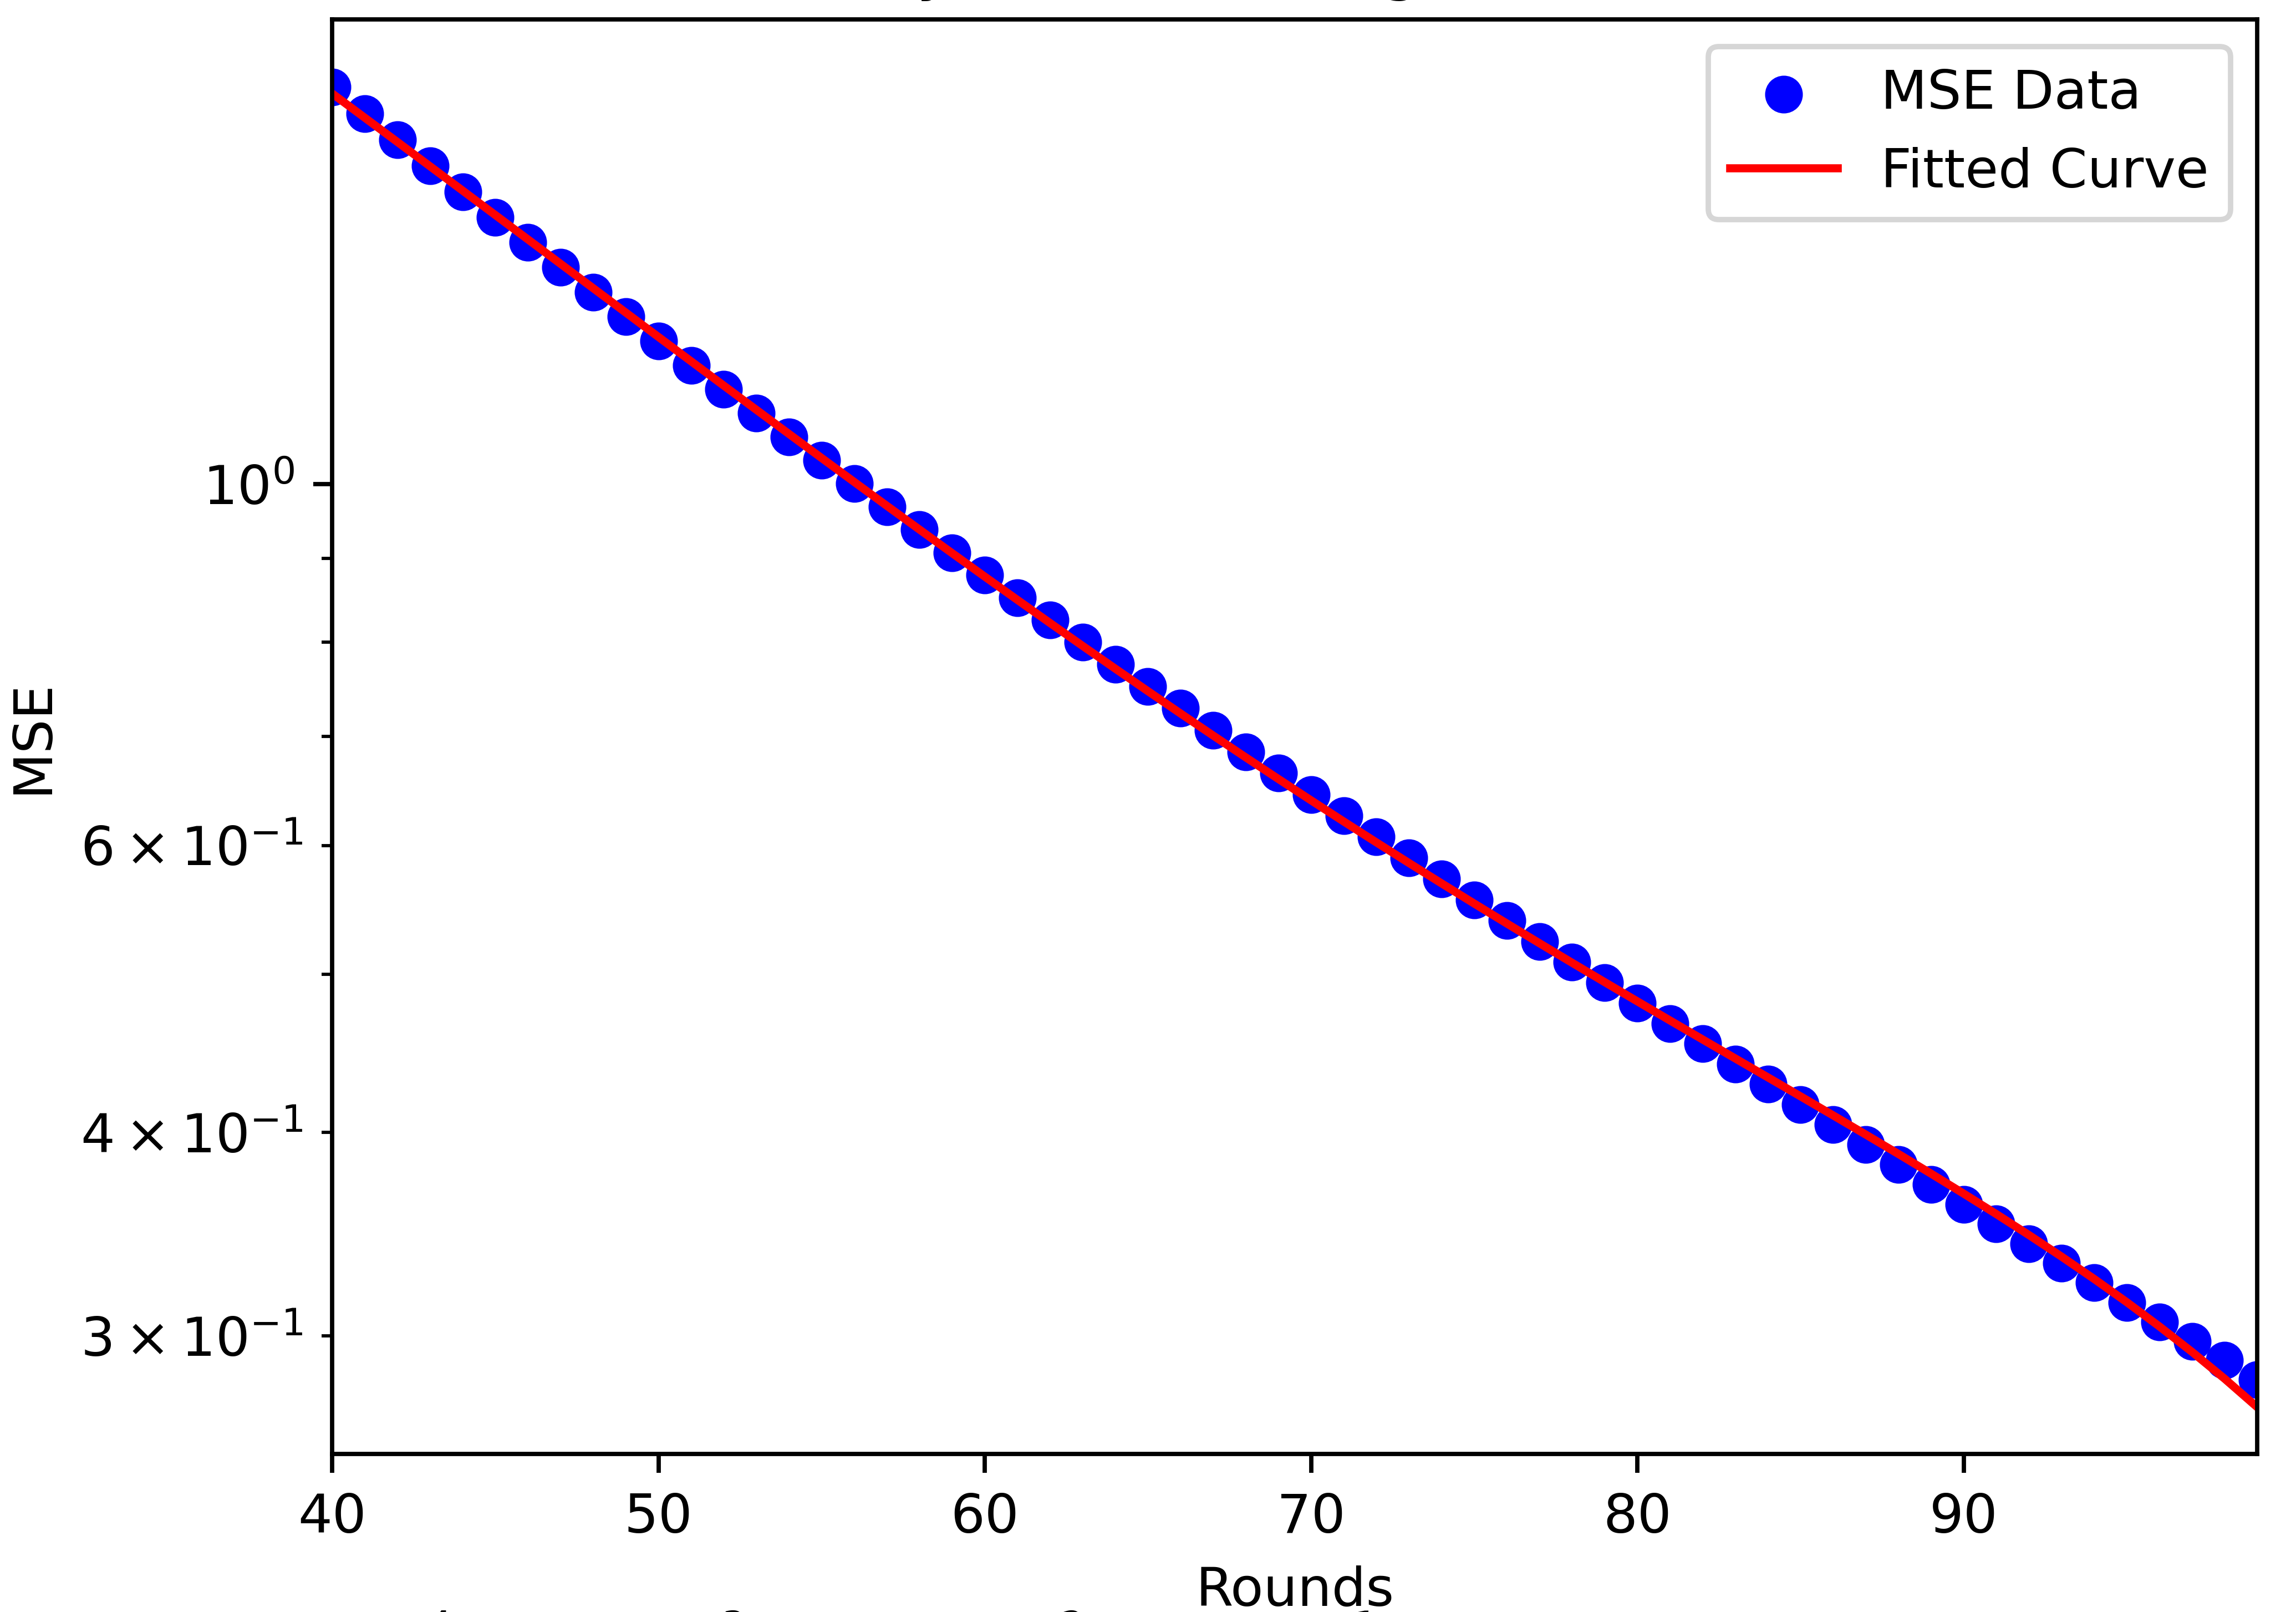
\includegraphics[width=0.49\linewidth]{figures/Simulation_outcomes/TorusGridGraph/DAB/DAB_modelfitting_rounds_99_model_2.png}}
     \caption{Torus Grid - polynomial regression fit - DAB; rounds 10-39 and 40-100}
         \label{fig:dabTorusModelFit}
 \end{figure}
 \begin{figure}[!ht]
     \centering
         \subfloat[]{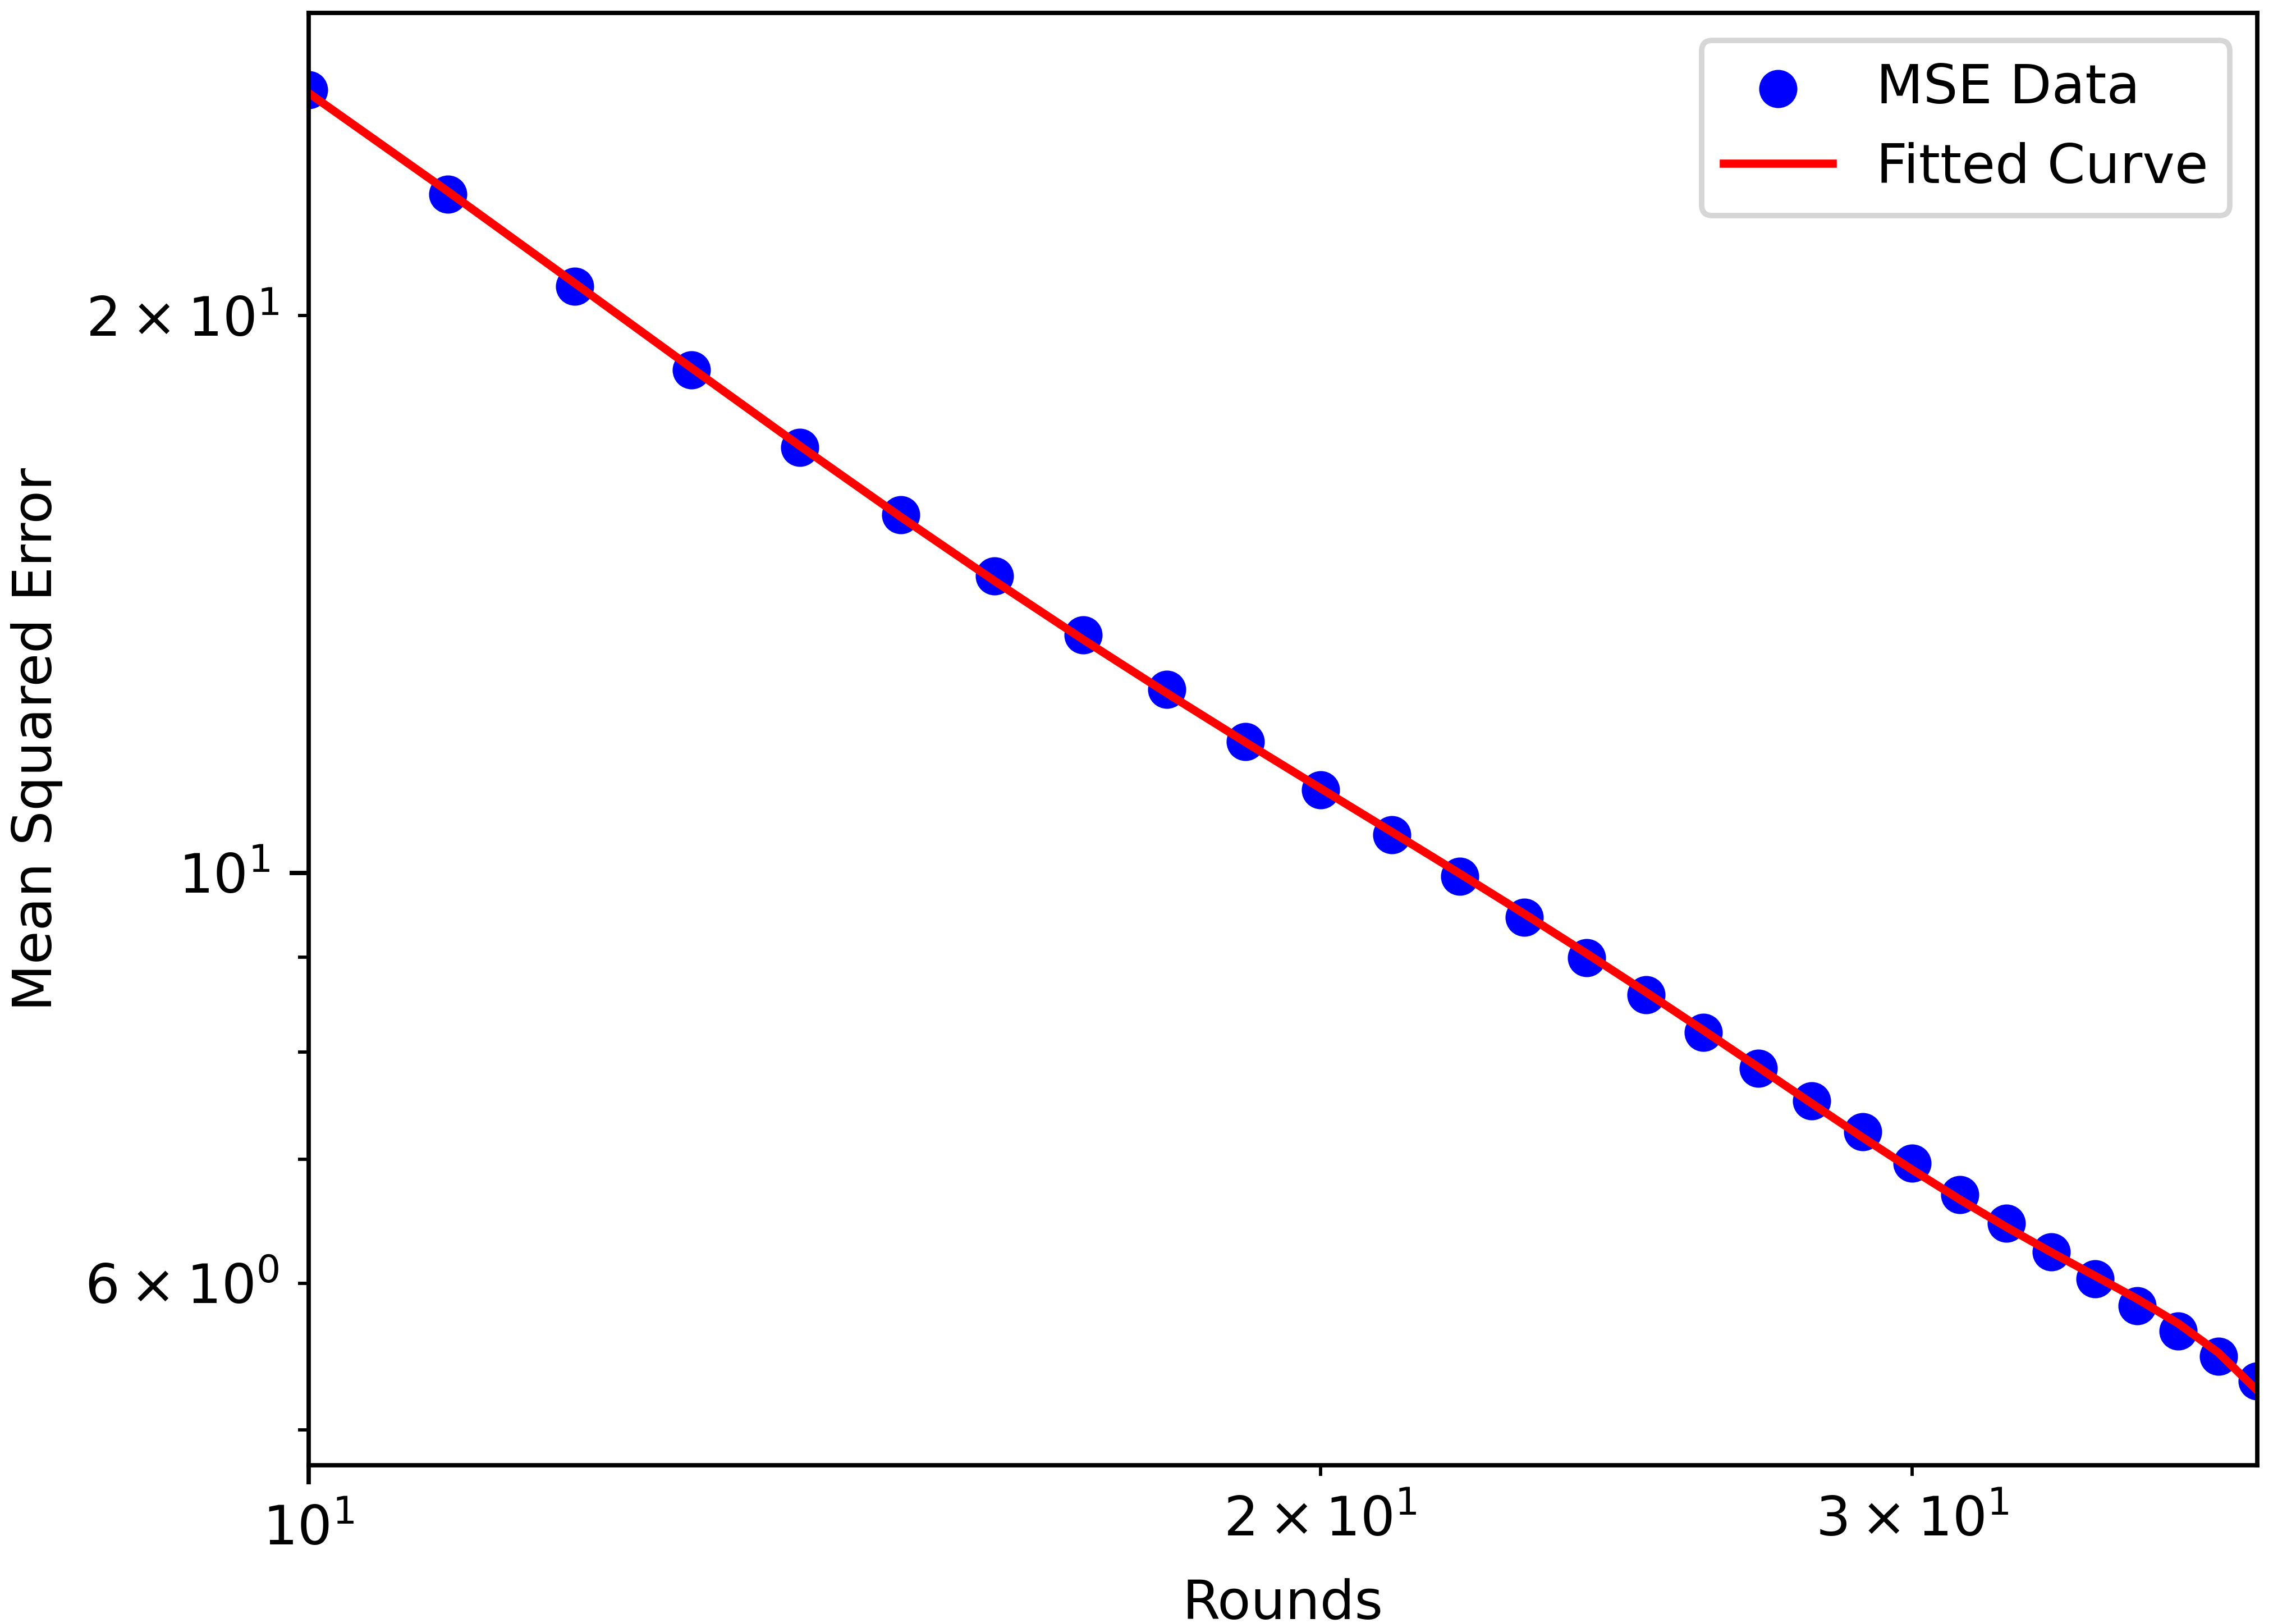
\includegraphics[width=0.49\linewidth]{figures/Simulation_outcomes/TorusGridGraph/PPS/PPS_modelfitting_rounds_38_model_2.png}}
     \hfil
         \subfloat[]{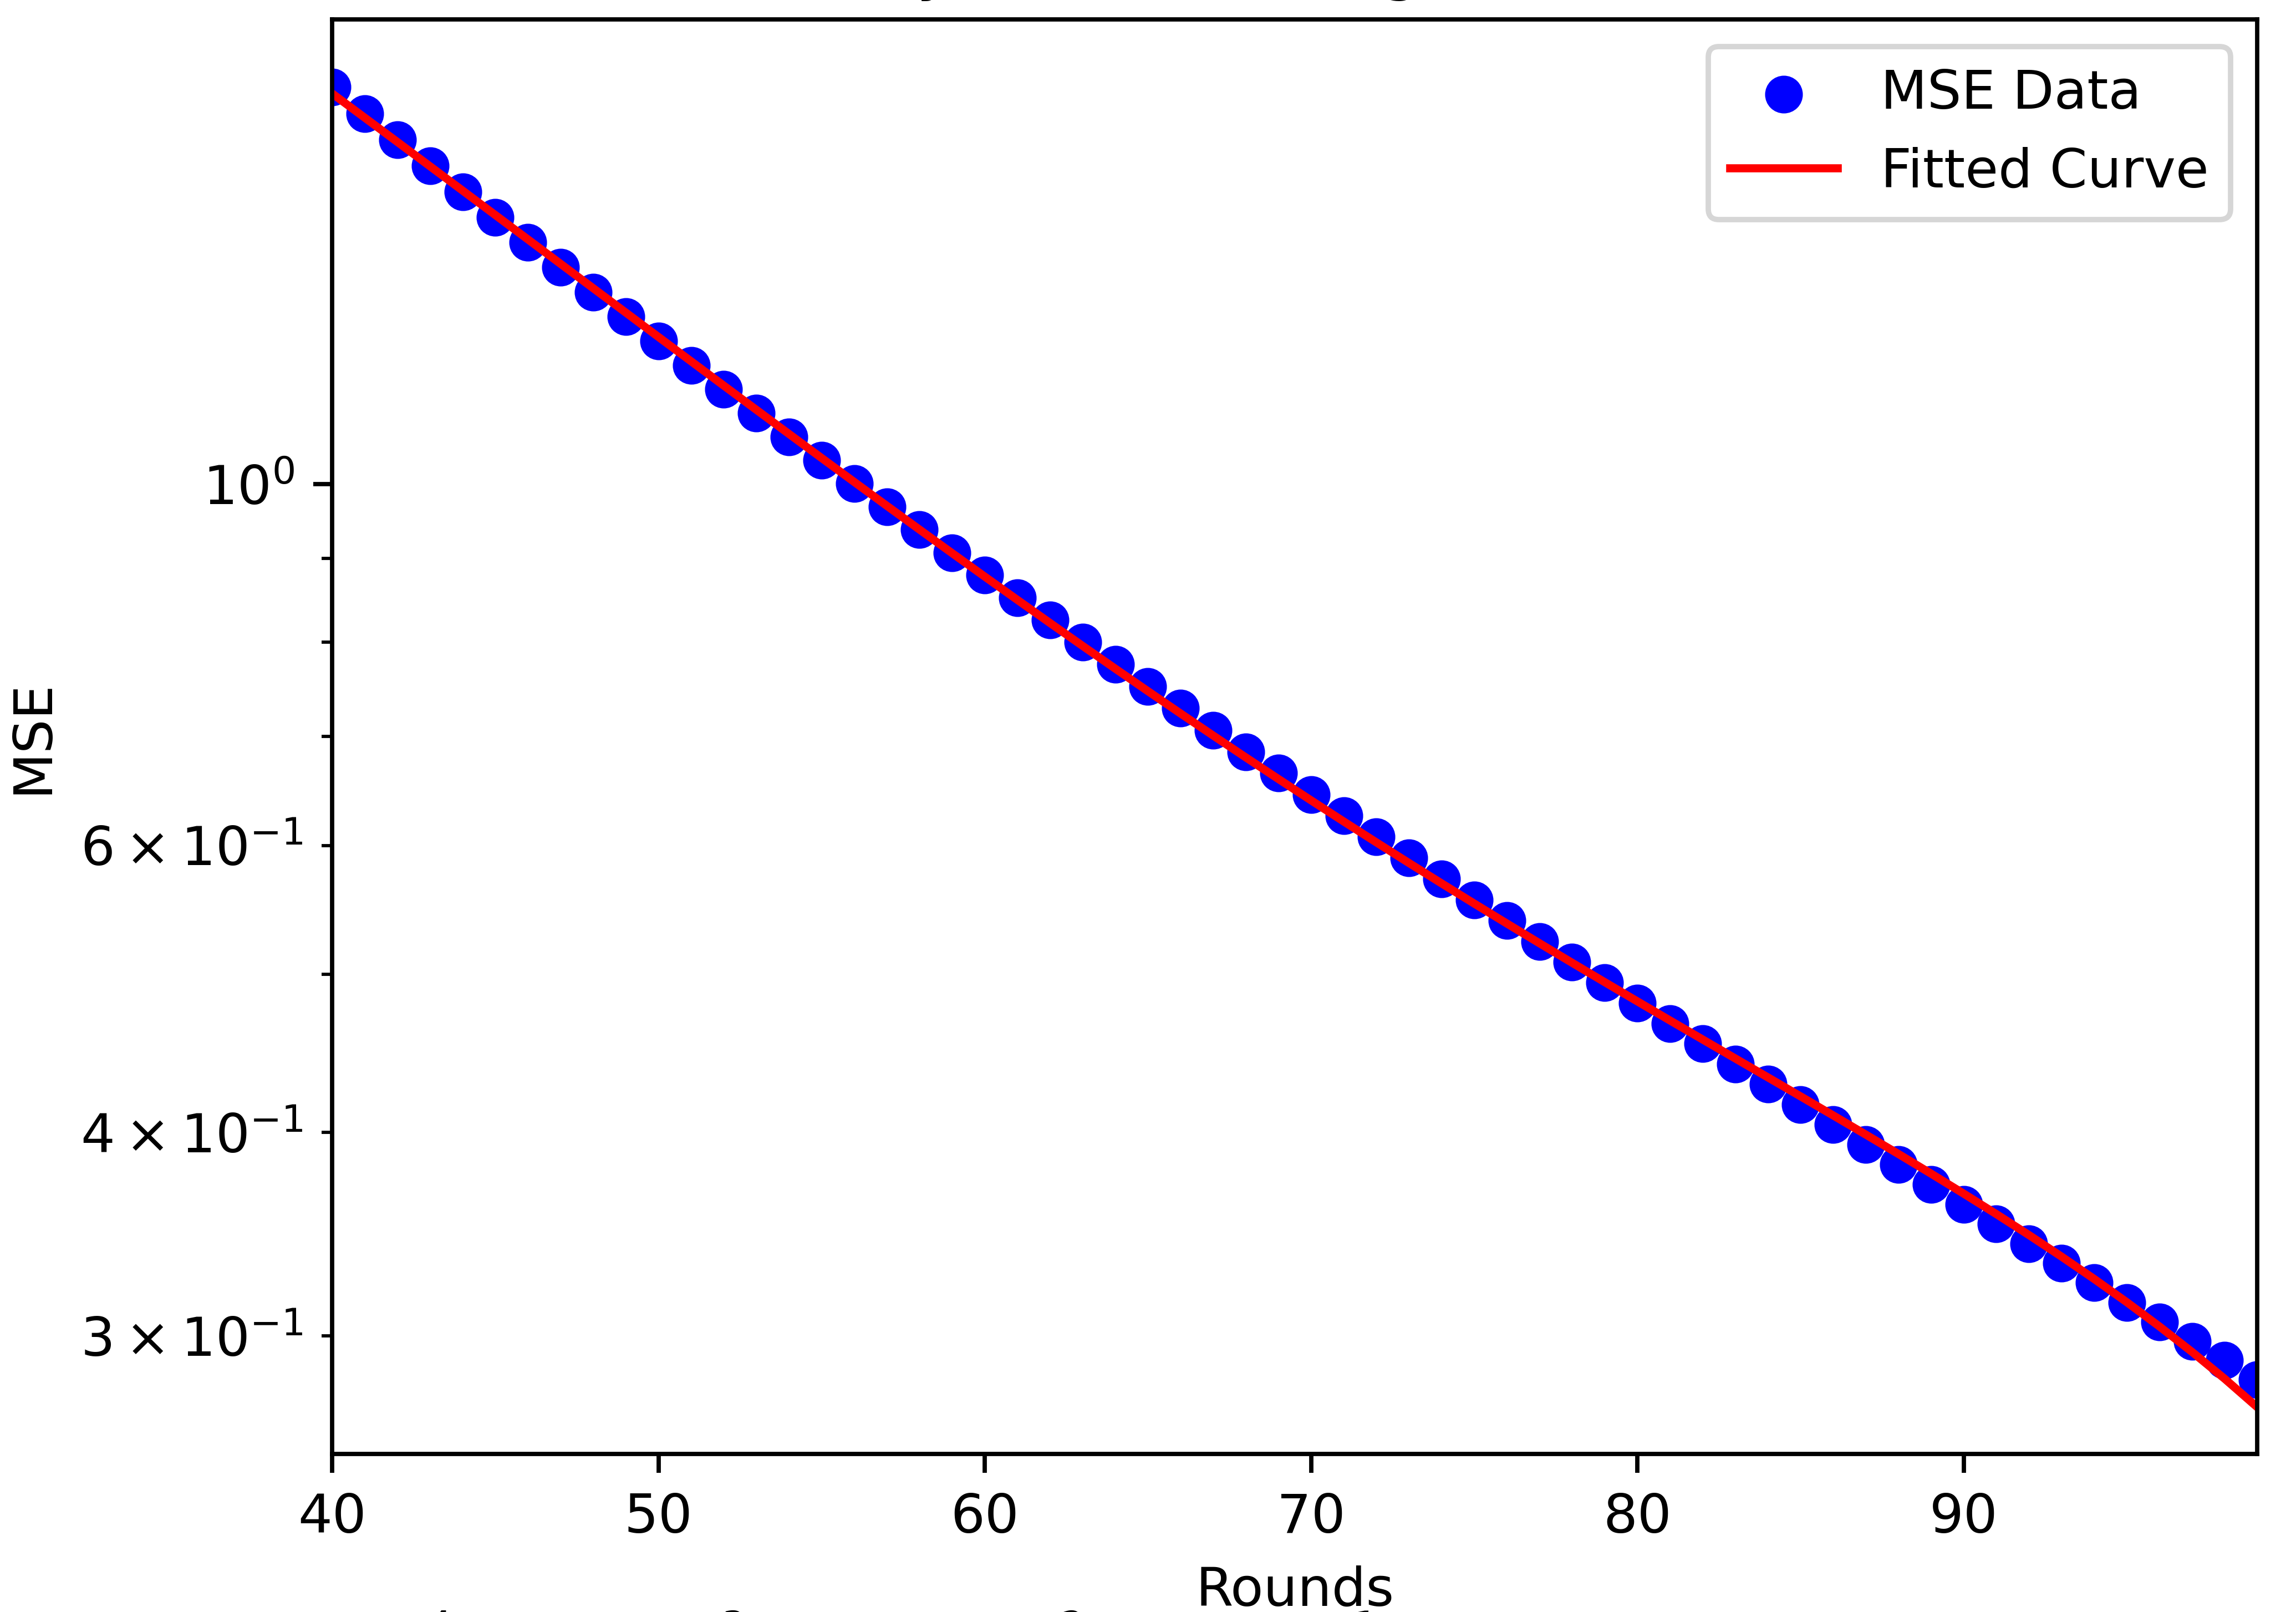
\includegraphics[width=0.49\linewidth]{figures/Simulation_outcomes/TorusGridGraph/DAB/DAB_modelfitting_rounds_99_model_2.png}}
     \caption{Torus Grid - polynomial regression fit - PPS; rounds 10-39 and 40-100}
         \label{fig:ppsTorusModelFit}
 \end{figure}
\begin{figure}[!ht]
    \centering
        \subfloat[]{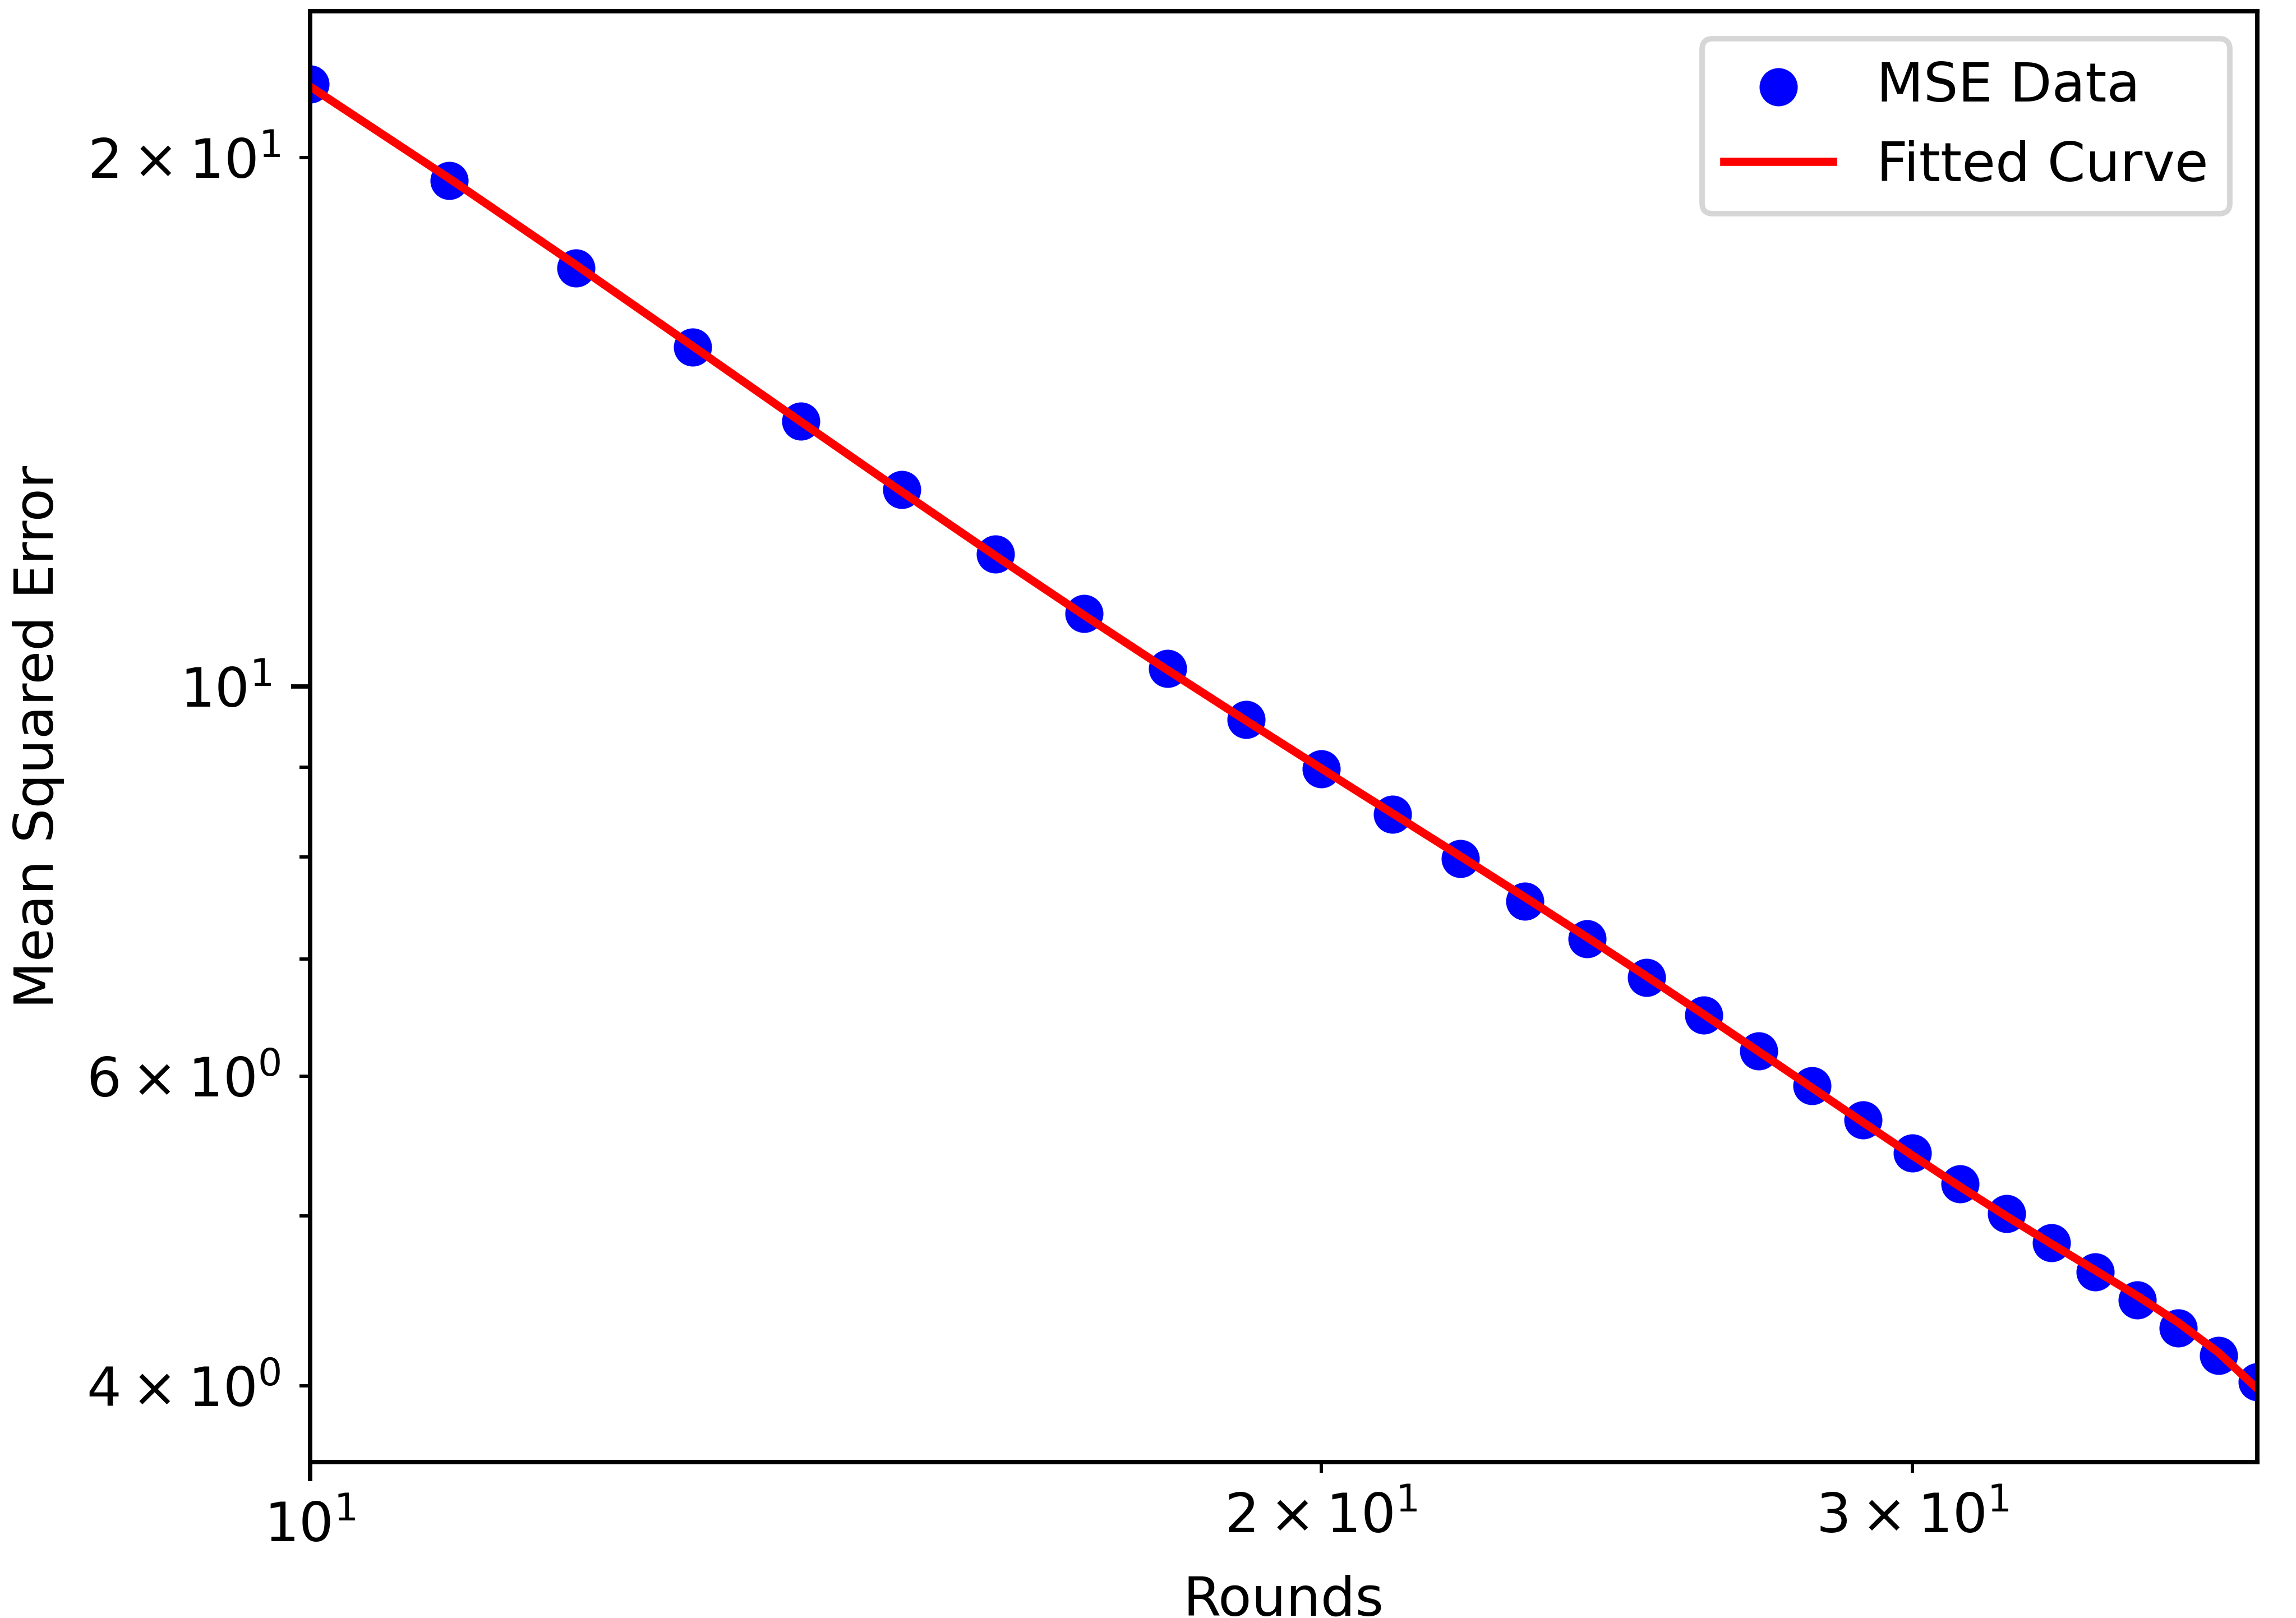
\includegraphics[width=0.49\linewidth]{figures/Simulation_outcomes/TorusGridGraph/ATPPS/ATPPS_modelfitting_rounds_38_model_2.png}}
    \hfil
        \subfloat[]{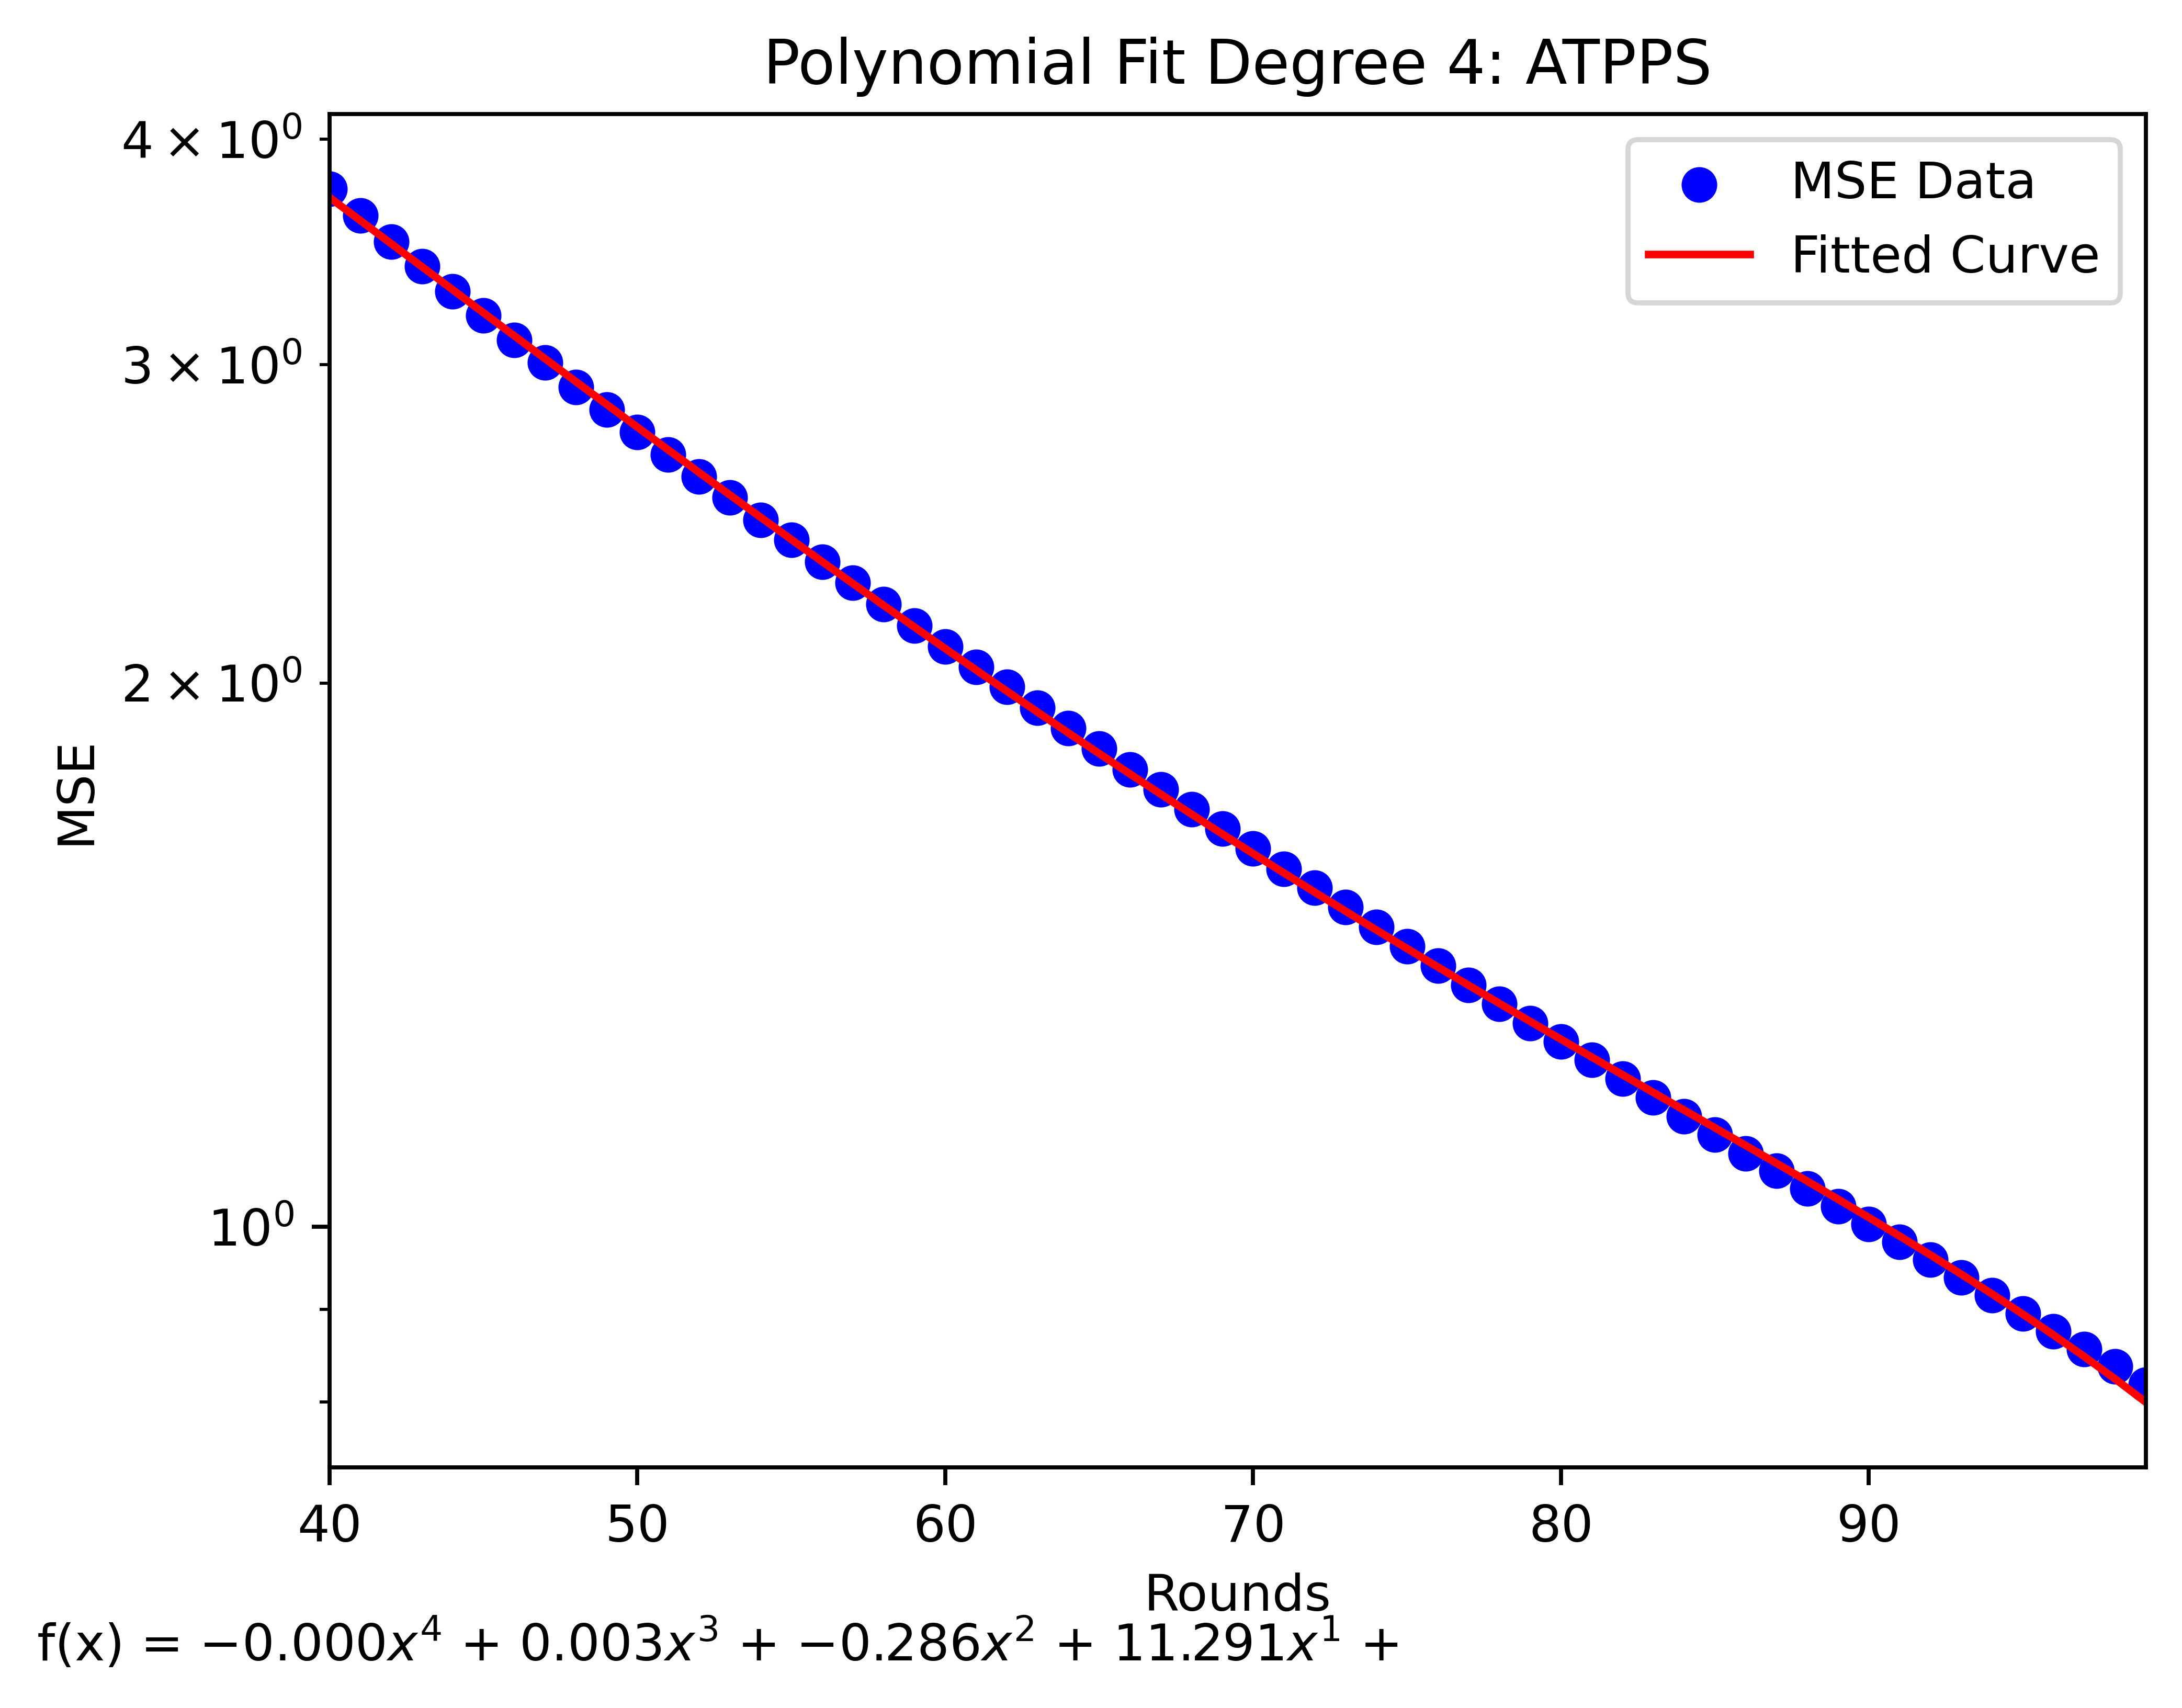
\includegraphics[width=0.49\linewidth]{figures/Simulation_outcomes/TorusGridGraph/ATPPS/ATPPS_modelfitting_rounds_99_model_2.png}}
    \caption{Torus Grid - polynomial regression fit - ATPPS; rounds 10-39 and 40-100}
        \label{fig:atppstorusModelFit}
\end{figure}
 \begin{figure}
     \centering
     \scalebox{0.8}{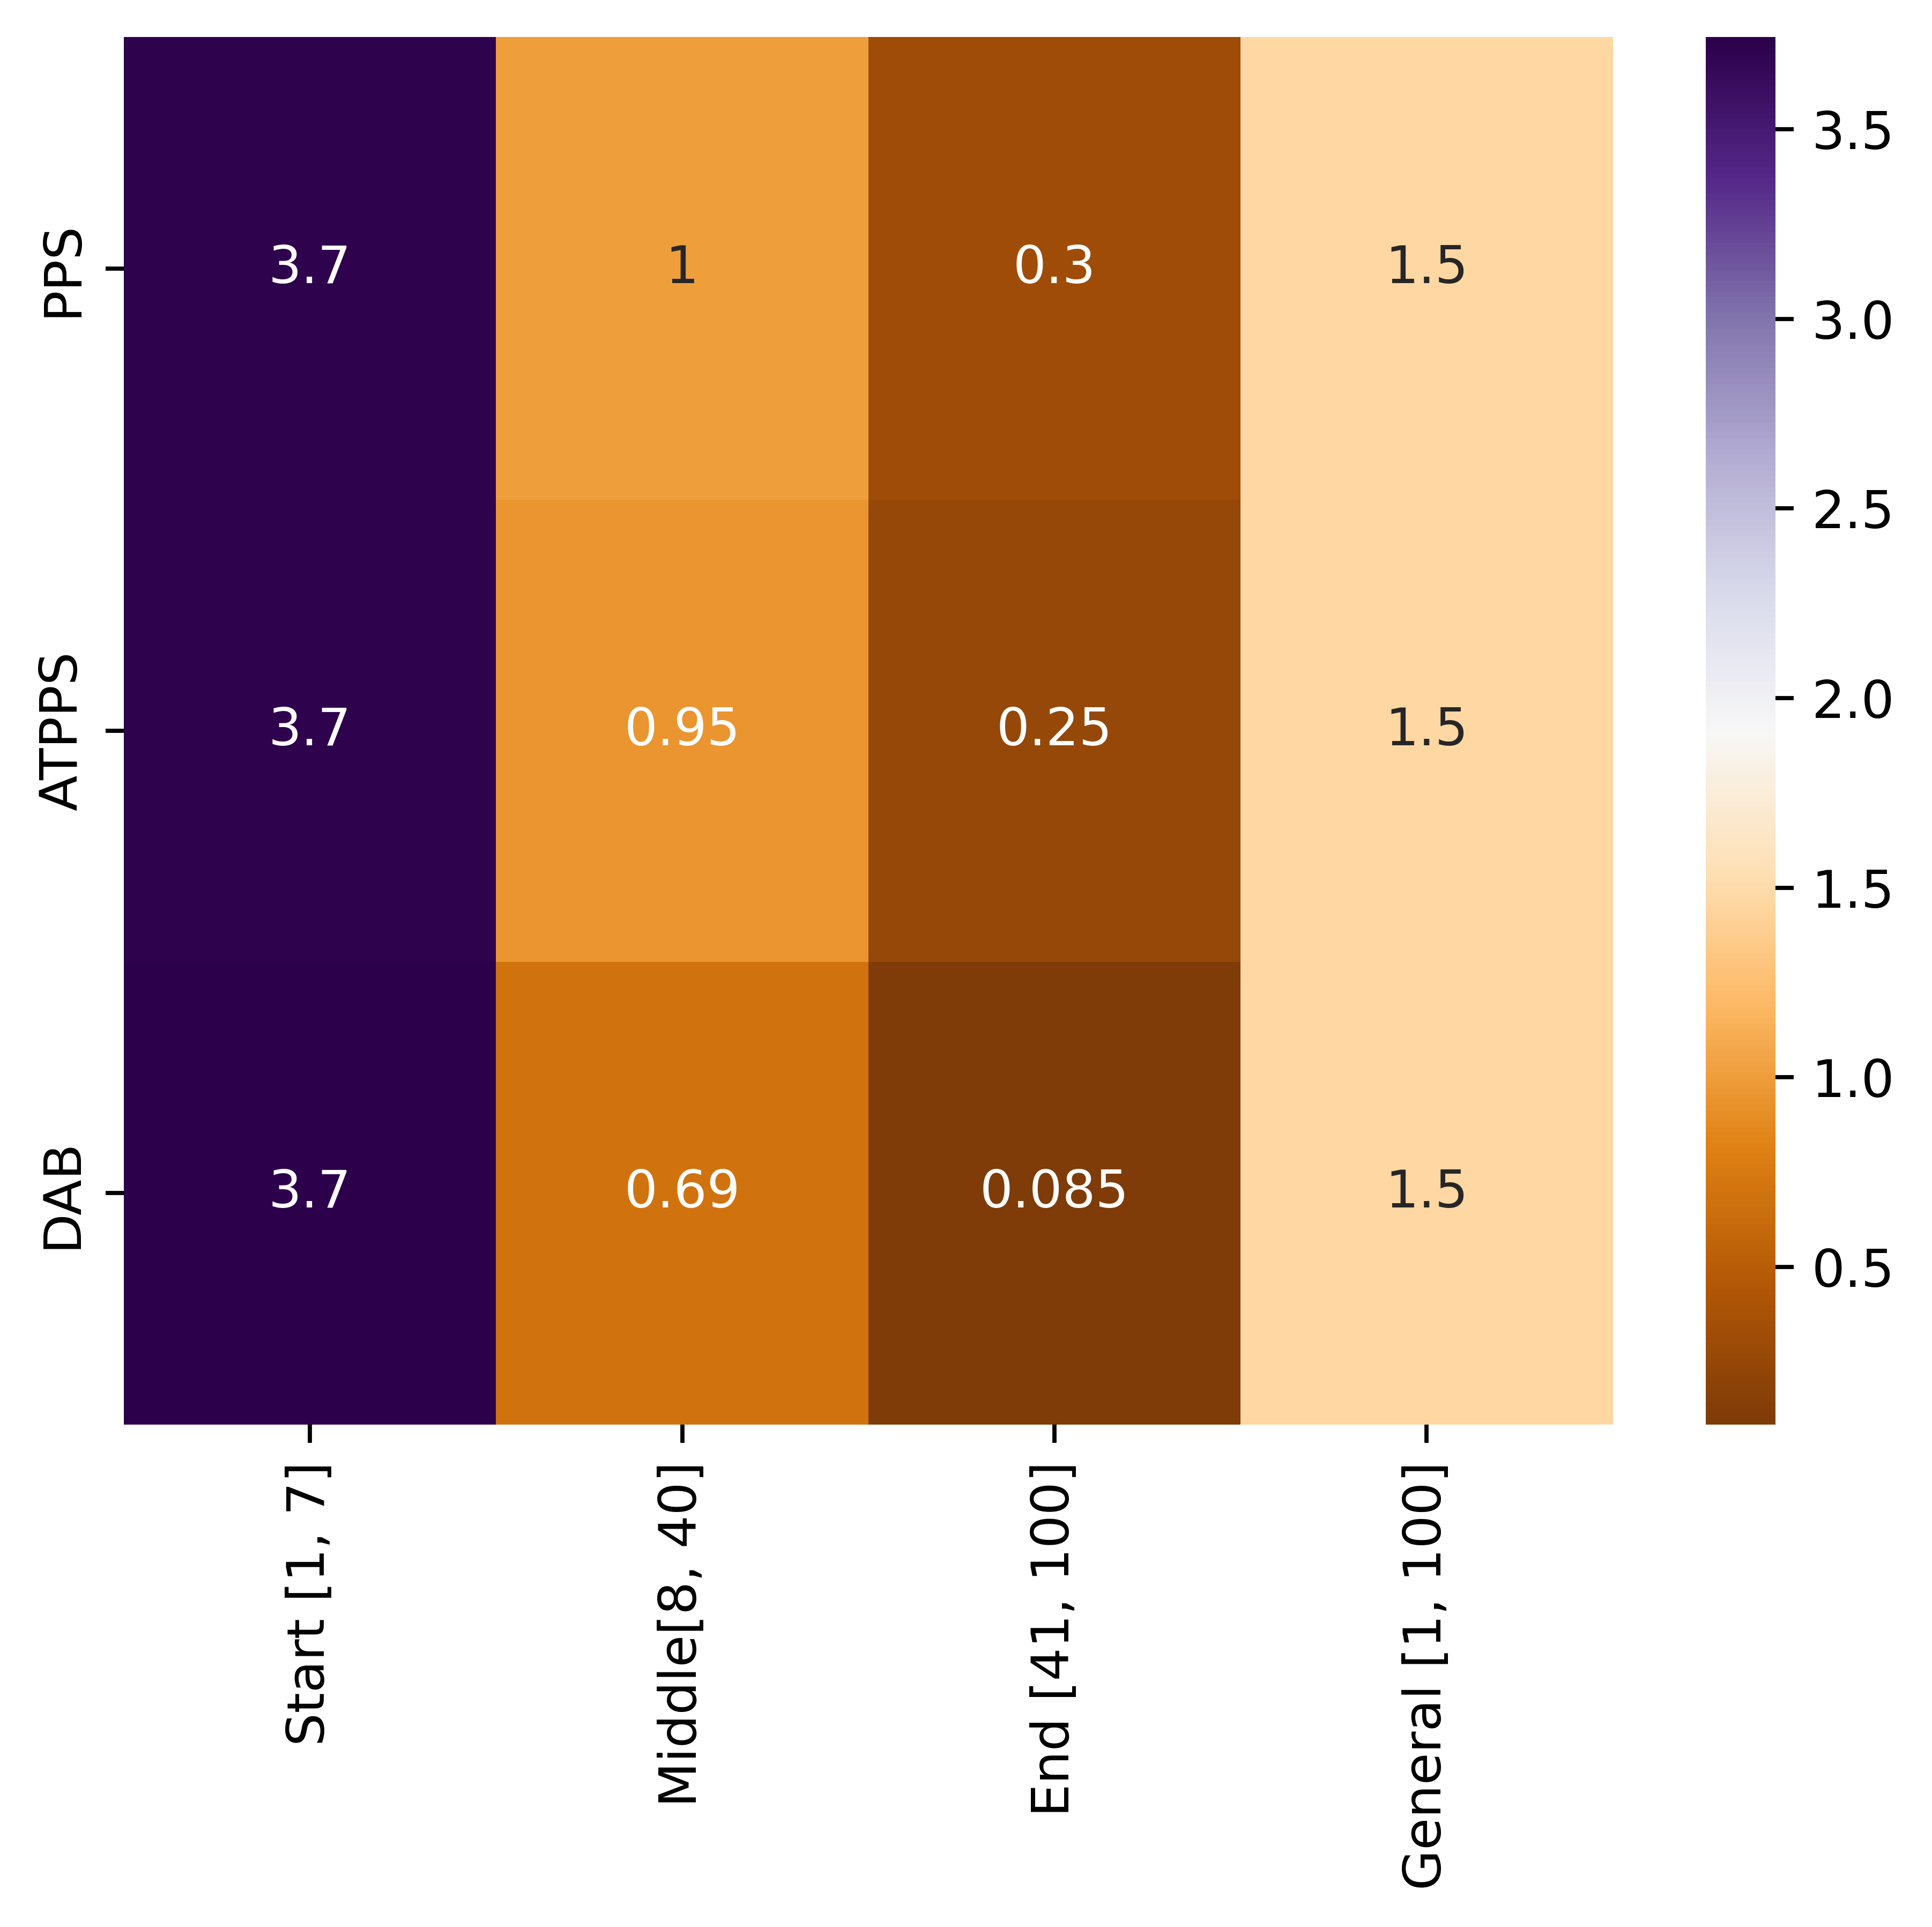
\includegraphics{figures/Simulation_outcomes/TorusGridGraph/DAB_vs_PPS_vs_ATPPS_slopesheatmap_100rounds_log_log.png}}
     \caption{Torus Grid - heat map of slopes per region - log-log}
     \label{fig:torusgraphslopes}
 \end{figure}

 \section{Lollipop Graph}\label{sec:lollipopgraph}
\subsection{(512, 512)-Lollipop Graph}
Figure \ref{fig:lollipopgraphMSEperRoundLogLog} displays the three curves of the load balancing algorithms. The ATPPS slightly outperforms the PPS, while the DAB underperforms compared to both Push-Pull Sum-based methods in reducing the error. The superior performance of PPS and ATPPS compared to DAB in the Lollipop graph $L_{512,512}$ can be explained by the structure of the graph and the fundamental differences in how these algorithms operate. The clique region is characterized by high connectivity and enables fast local balancing due to the low diameter for the Push-Pull Sum-based algorithms. The path region with low connectivity slows down information propagation and balancing for the Push-Pull Sum-based algorithms and favors the deterministic DAB. The initial discrepancy between the DAB and the Push-Pull Sum-based algorithms in the first 10 rounds arises due to the fast error reduction achieved by PPS and ATPPS within the clique. The DAB struggles to perform well for cliques, as observed in section \ref{sec:completeGraph}. DAB performs rather well in the Path graph which in theory is similar to the Ring graph without the edge connecting the first and last nodes as described in section \ref{sec:ringgraph}. It prioritizes nodes with the least load, which can lead to inefficient propagation along the clique. DAB does not exploit the random spreading mechanism of the Push-Pull Sum-based algorithms. The Push-Pull Sum-based algorithms achieve a steep downward slope with value -1.3 between rounds 1 and 7, while the DAB achieves a value of -0.34 (figure \ref{fig:lollipopslopes}). In the mid-to-late phase, the slope flattens for both Push-Pull Sum-based algorithms. This is evident from the slope values dropping to as low as $-0.56$ for PPS and $-0.57$ for ATPPS. In this phase, the path section of the Lollipop graph dominates the residual imbalances. The ATPPS achieves nearly identical behavior to the PPS in the early rounds, as it starts with similar strategies where the threshold is relatively easy to surpass as the load differences in the network are still very high. ATPPS outperforms the PPS slightly in the later rounds due to its ability to dynamically adjust its balancing strategy based on the current state of load imbalances. This allows it to better address residual imbalances in the path section of the Lollipop graph as showcased in section \ref{sec:ringgraph}.

The MSE data for the DAB is best described by a polynomial of degree 3, following the equation:
\begin{align}
    MSE_r=-5.89\times10^{-5}r^{3}+0.03r^{2}-5.68r+459.42    
\end{align}
as shown in figure \ref{fig:dablollipopgraphModelFit}. The MSE trends for the PPS and ATPPS algorithms are better captured by polynomials of degree 4. The best-fit equation for the PPS model is:
\begin{align}
    MSE_r=8.44\times 10^{-7}r^{4}-2.52\times 10^{-4}r^{3}-0.03r^{2}-1.64r+56.68    
\end{align}
(figure \ref{fig:ppslollipopgraphModelFit}) and the ATPPS model fit follows the equation:
\begin{align}
    MSE_r=8.69 \times 10^{-7}r^{4}-2.56 \times 10^{-4}r^{3}+0.03r^{2}-1.62r+54.48    
\end{align}
(figure \ref{fig:atppslollipopgraphModelFit}).

\begin{figure}[]
    \centering
    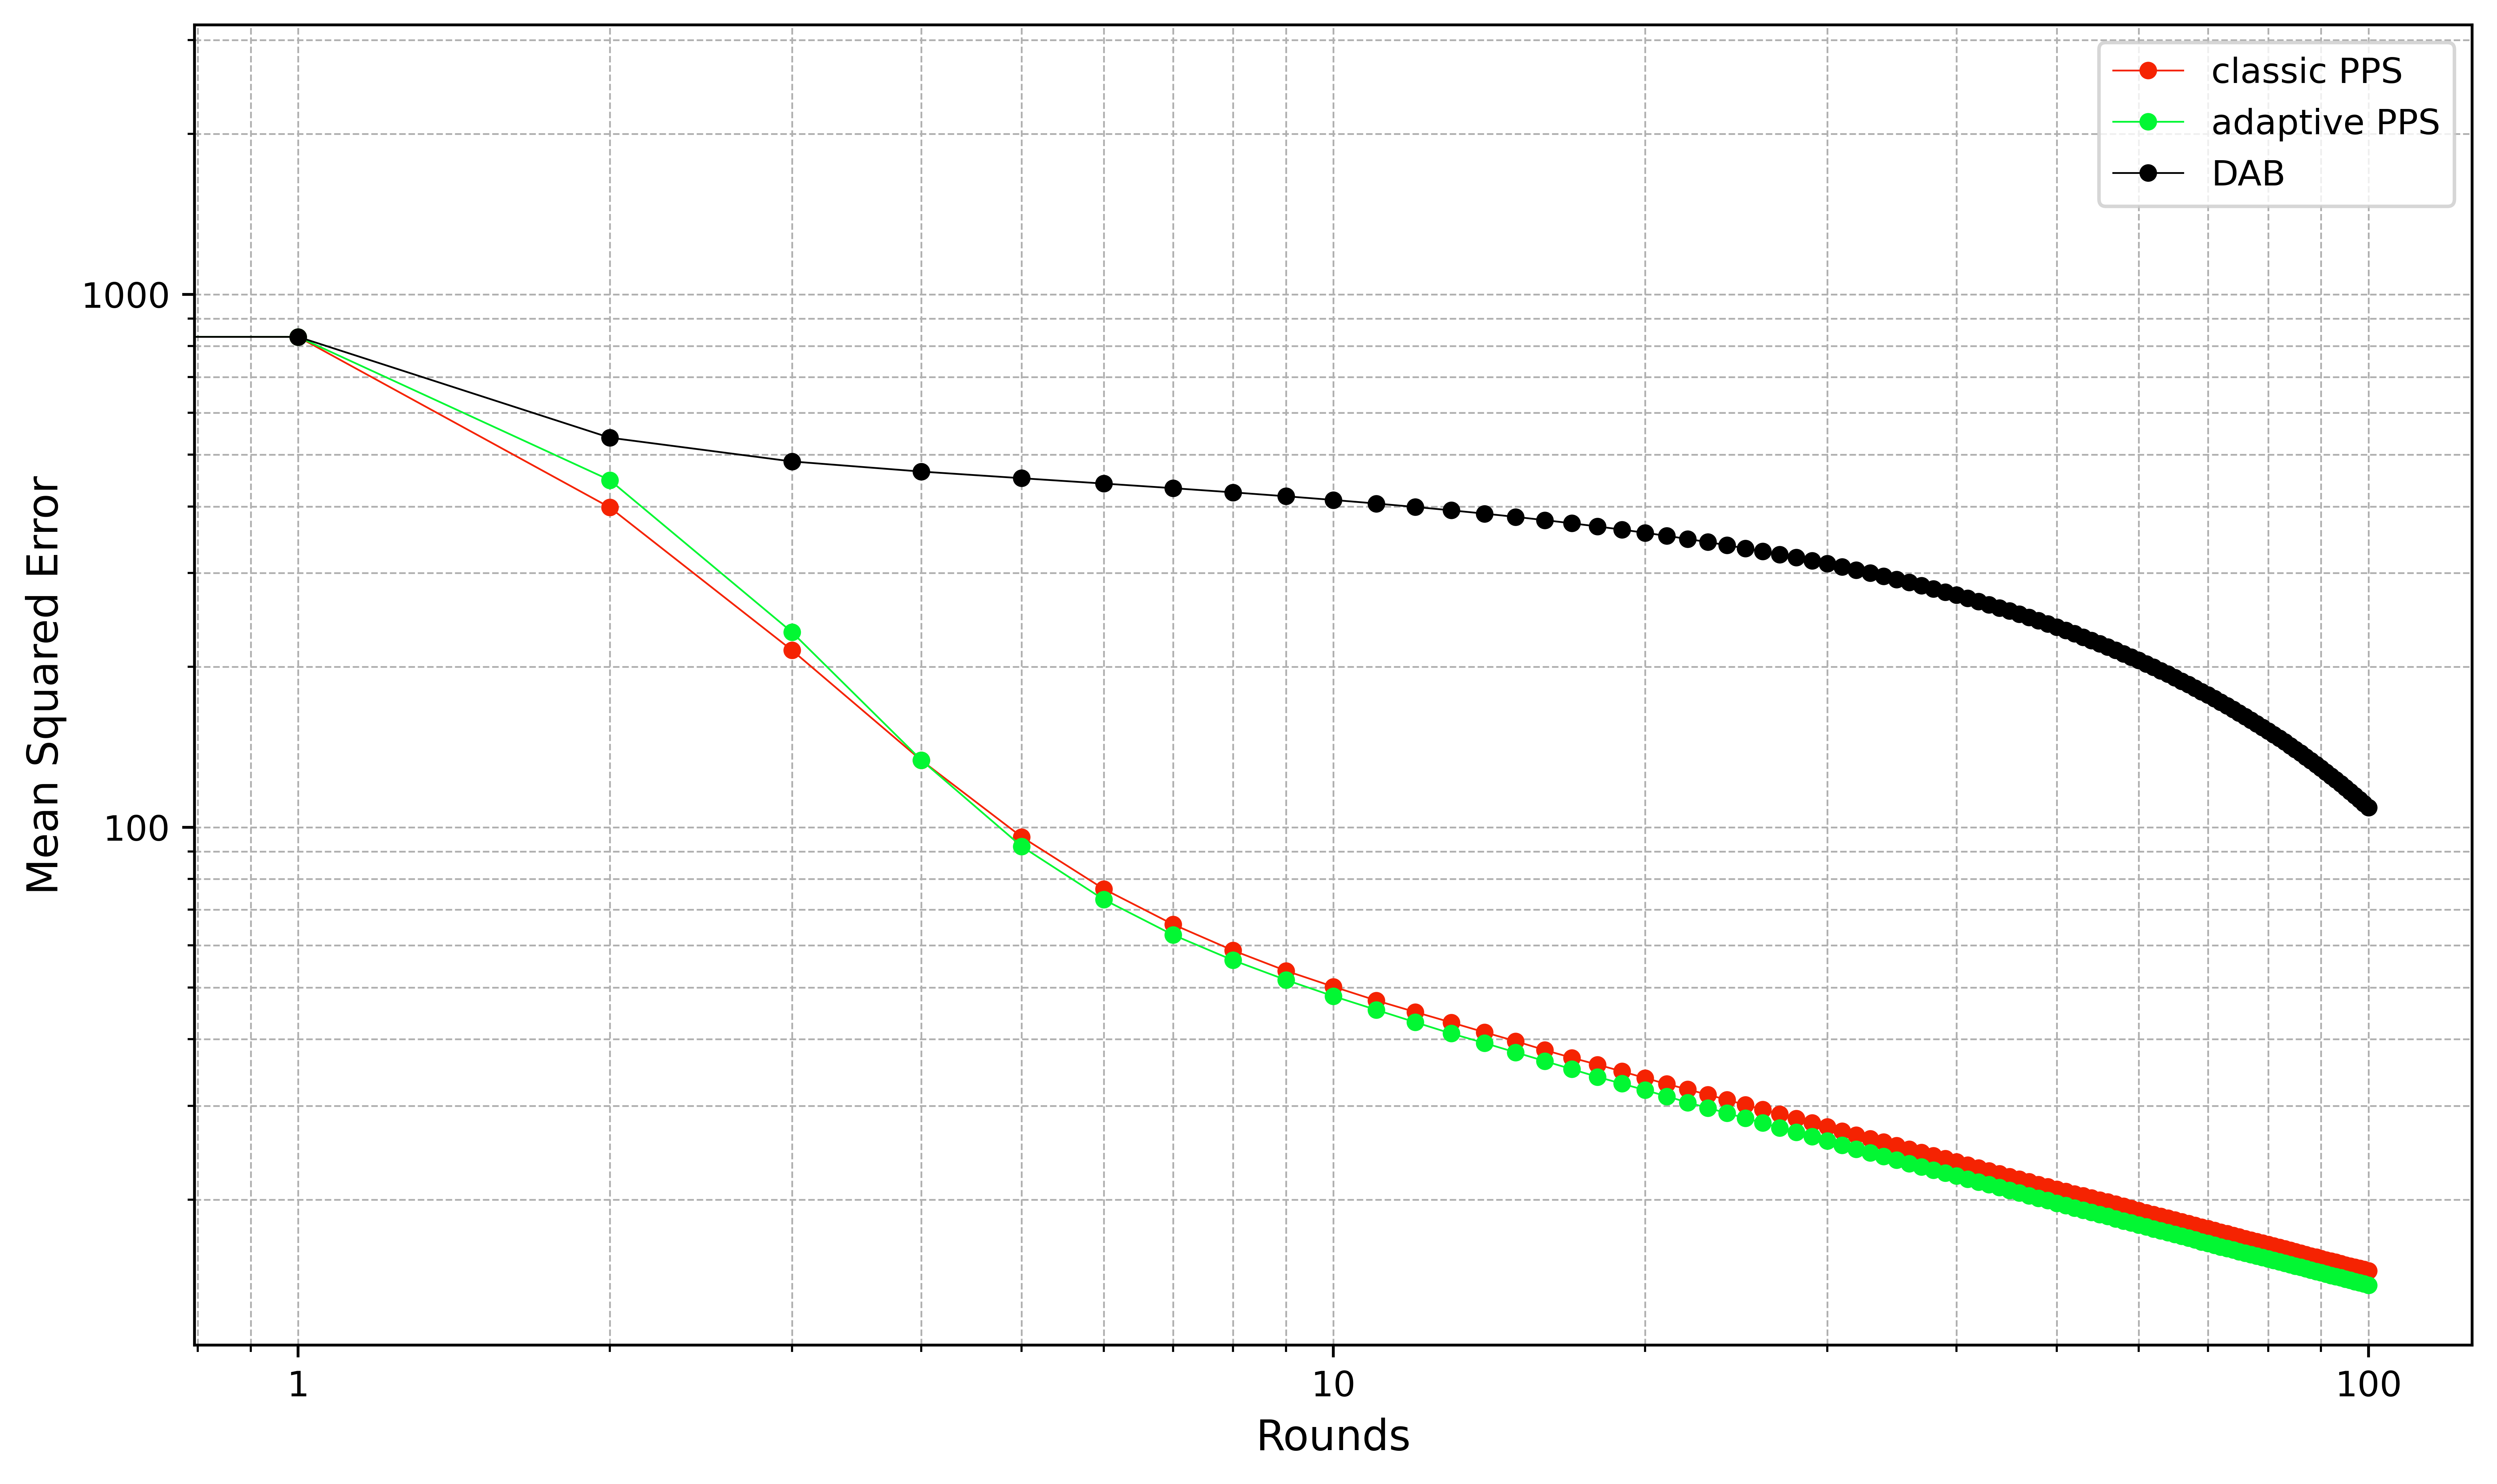
\includegraphics[width=\linewidth]{figures/Simulation_outcomes/LollipopGraph/512_512/DAB_vs_PPS_LG_r100_n1024_averaged_loglog.png}
    \caption{(512, 512)-Lollipop graph - mean squared error per rounds - log-log}
    \label{fig:lollipopgraphMSEperRoundLogLog}
\end{figure}

\begin{figure}[]
    \centering
    \scalebox{0.8}{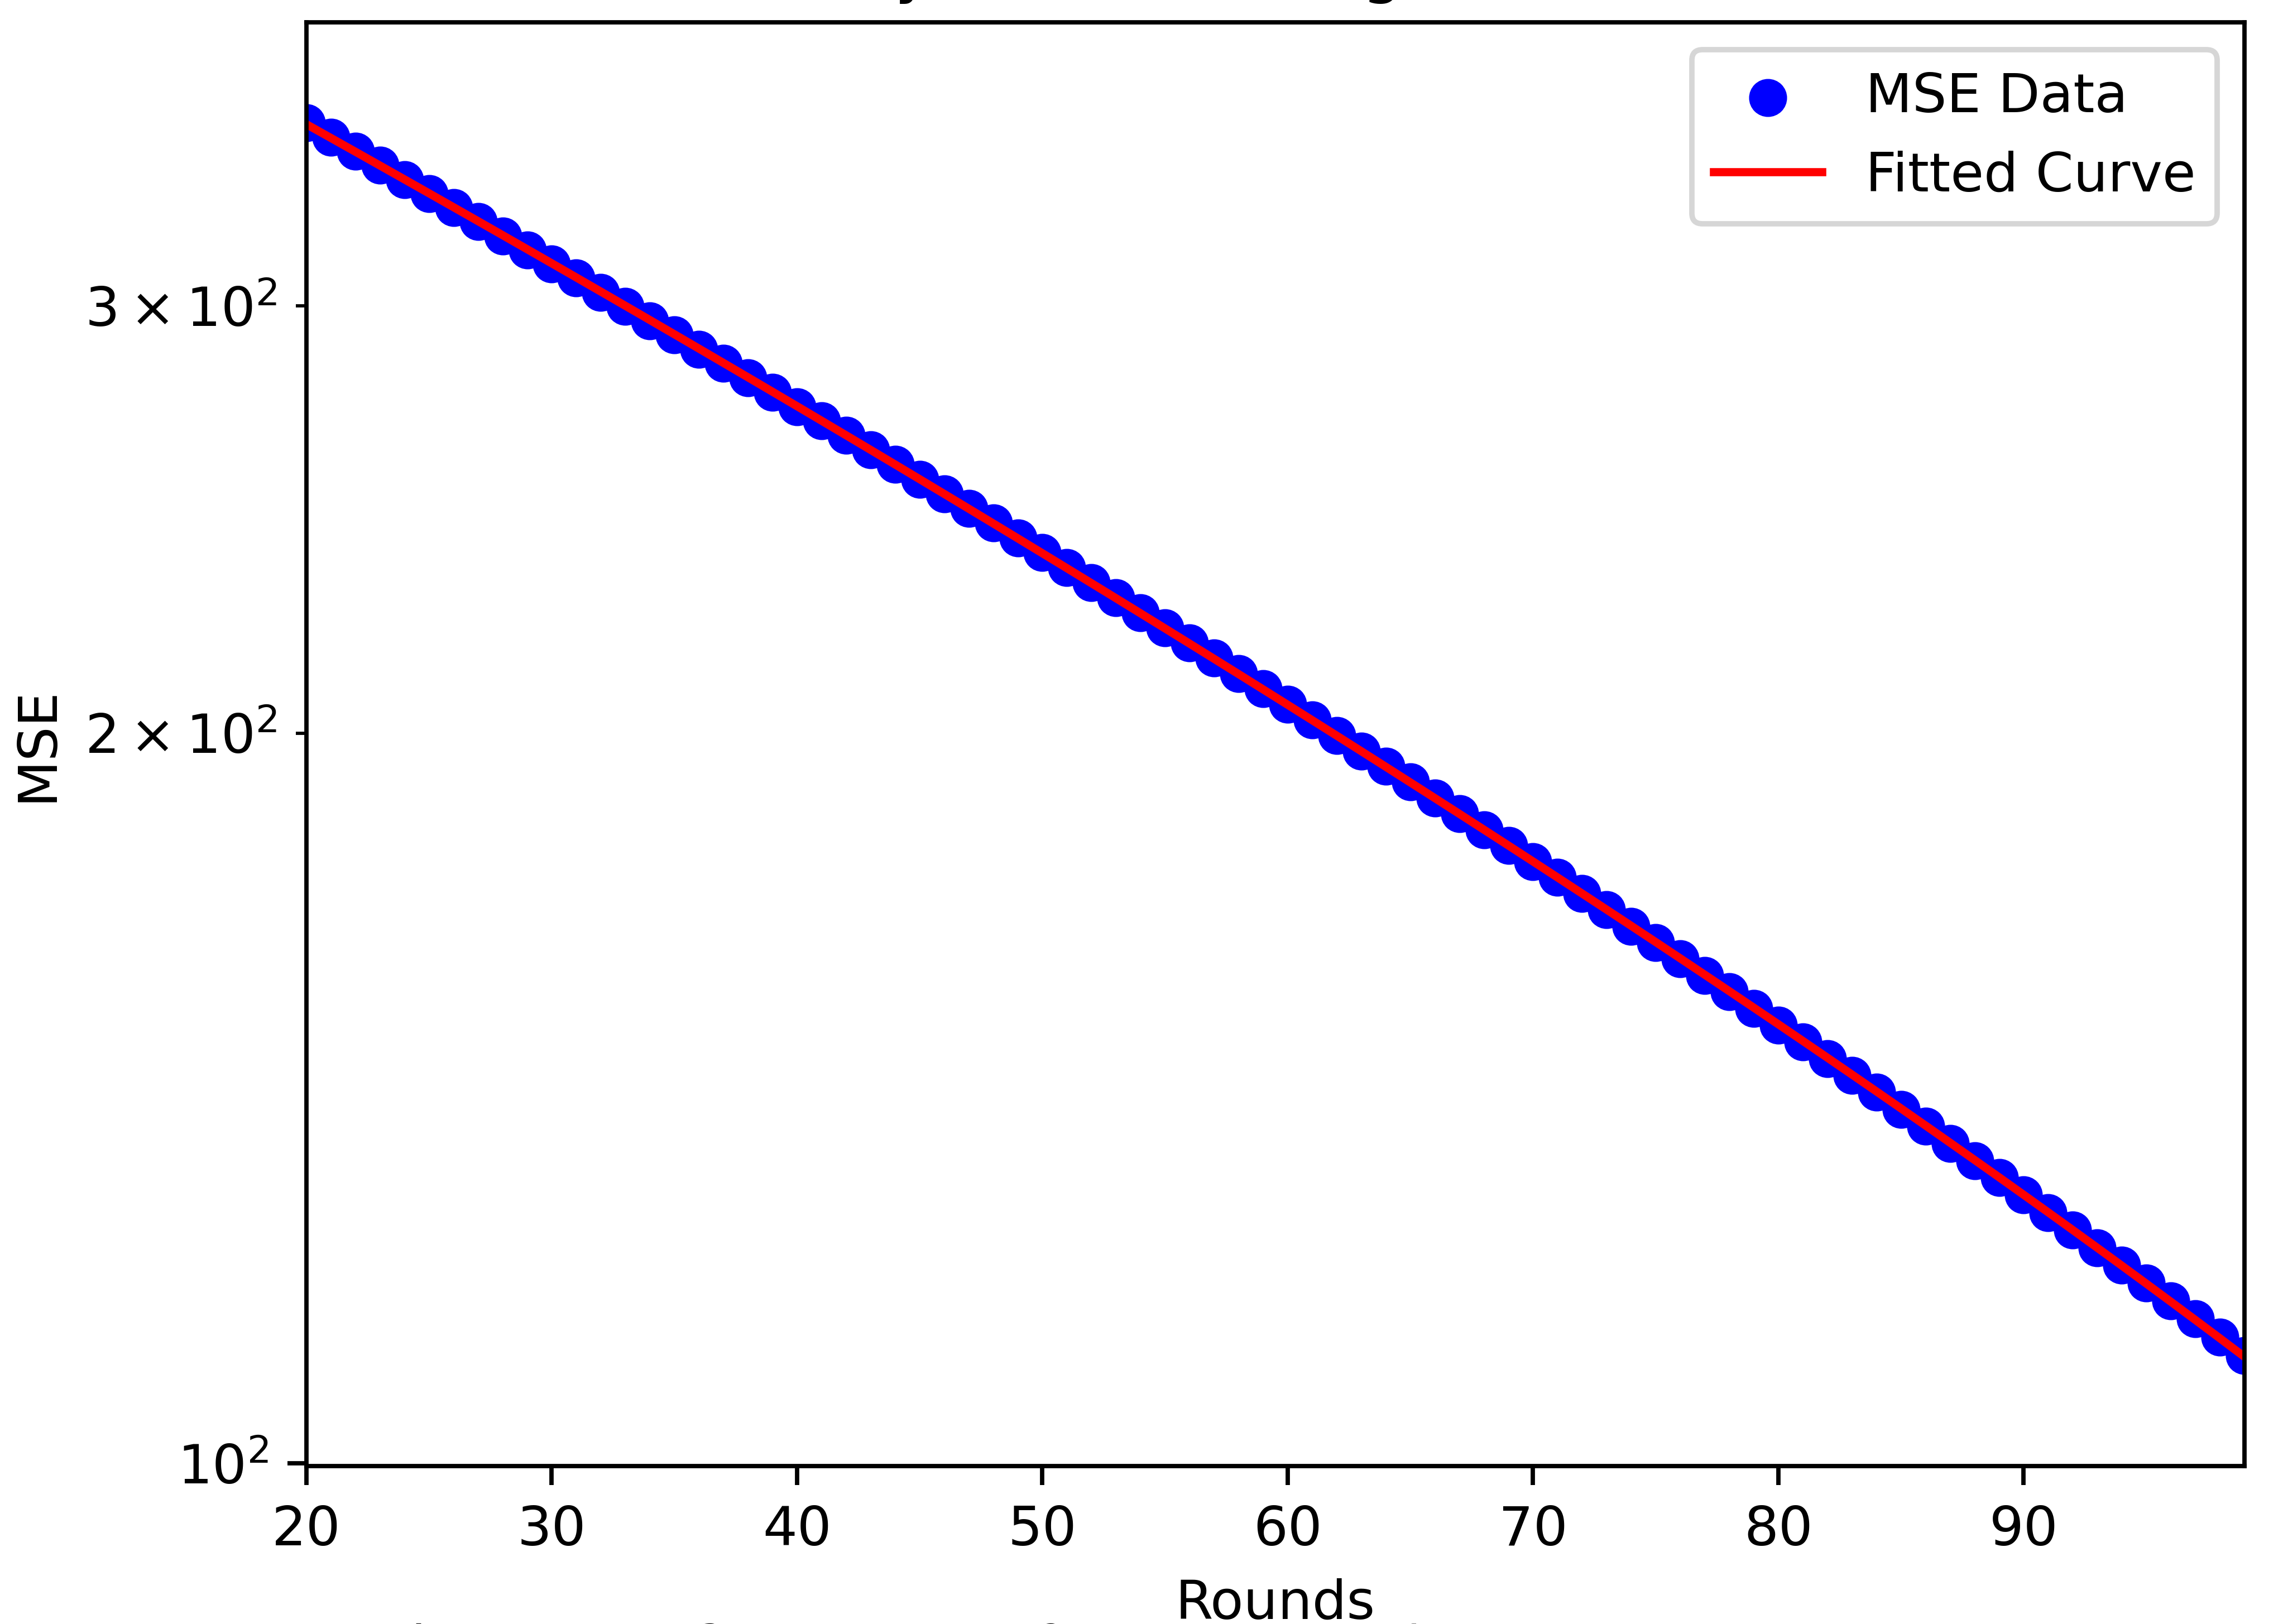
\includegraphics{figures/Simulation_outcomes/LollipopGraph/512_512/DAB/DAB_modelfitting_rounds_99_model_2.png}}
    \caption{(512, 512)-Lollipop graph - polynomial regression fit - DAB}
    \label{fig:dablollipopgraphModelFit}
\end{figure}

\begin{figure}[]
    \centering
    \scalebox{0.8}{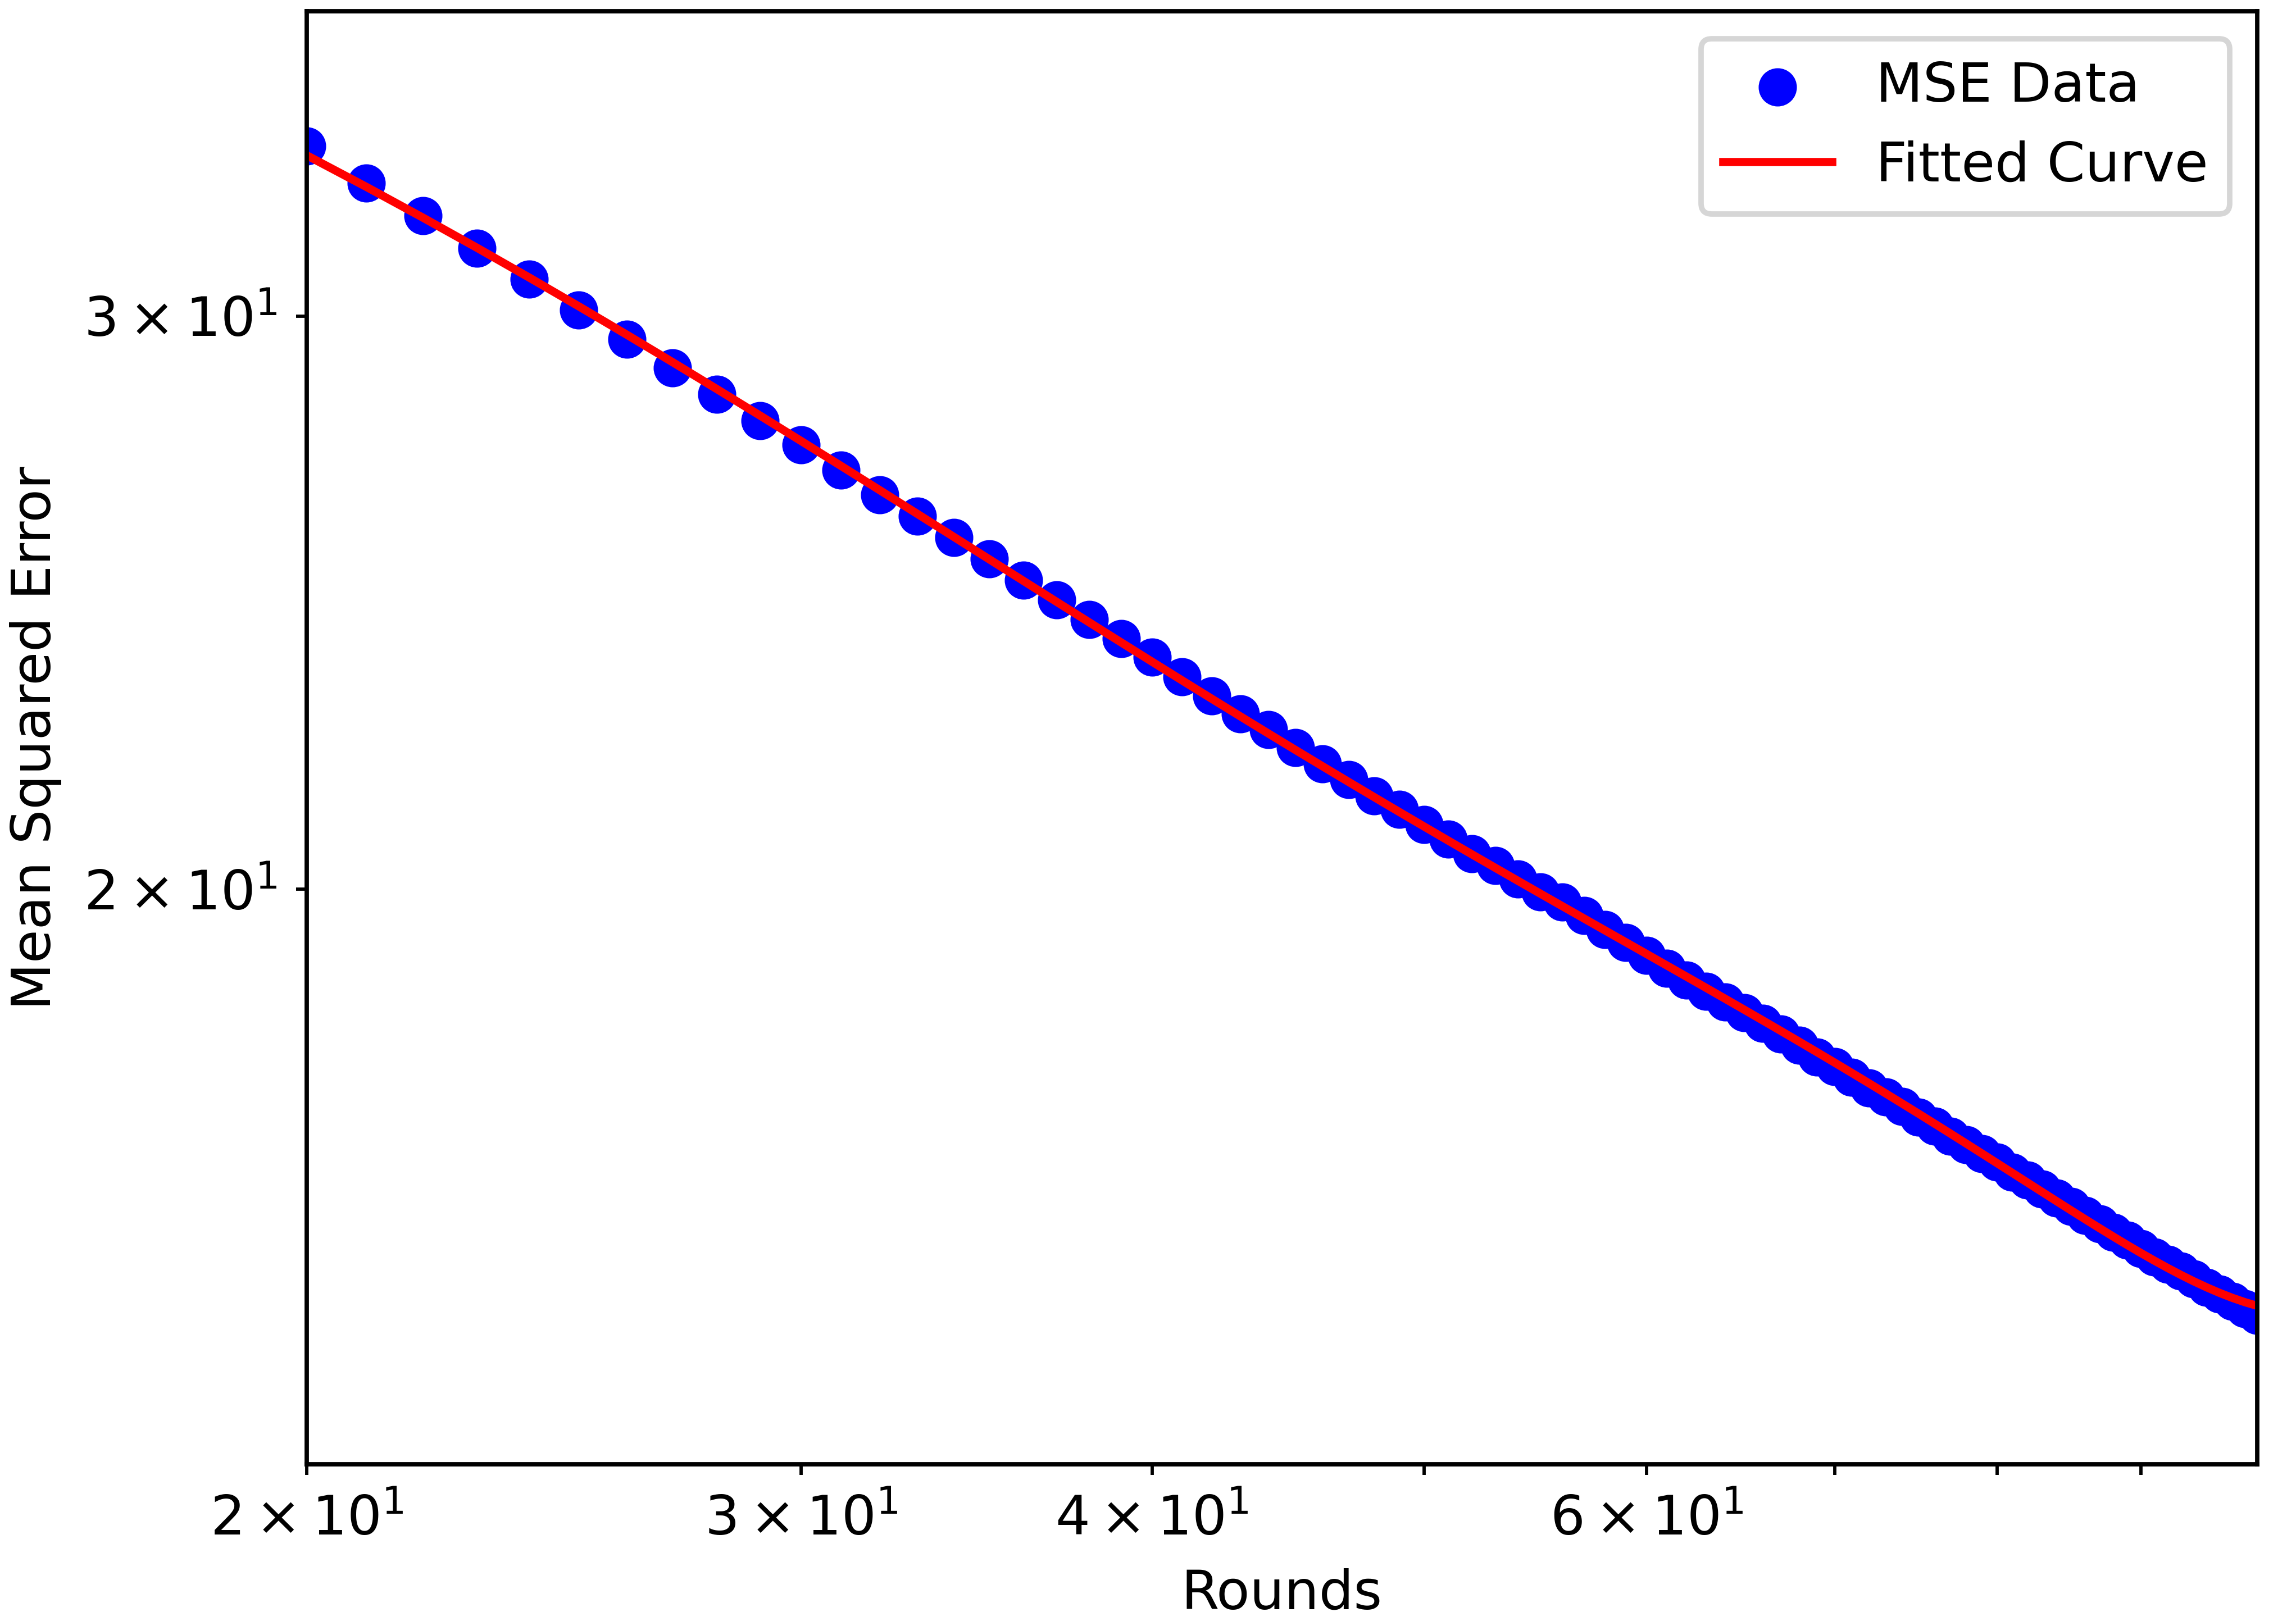
\includegraphics{figures/Simulation_outcomes/LollipopGraph/512_512/PPS/PPS_modelfitting_rounds_99_model_2.png}}
    \caption{(512, 512)-Lollipop graph - polynomial regression fit - PPS}
    \label{fig:ppslollipopgraphModelFit}
\end{figure}

\begin{figure}[]
    \centering
    \scalebox{0.8}{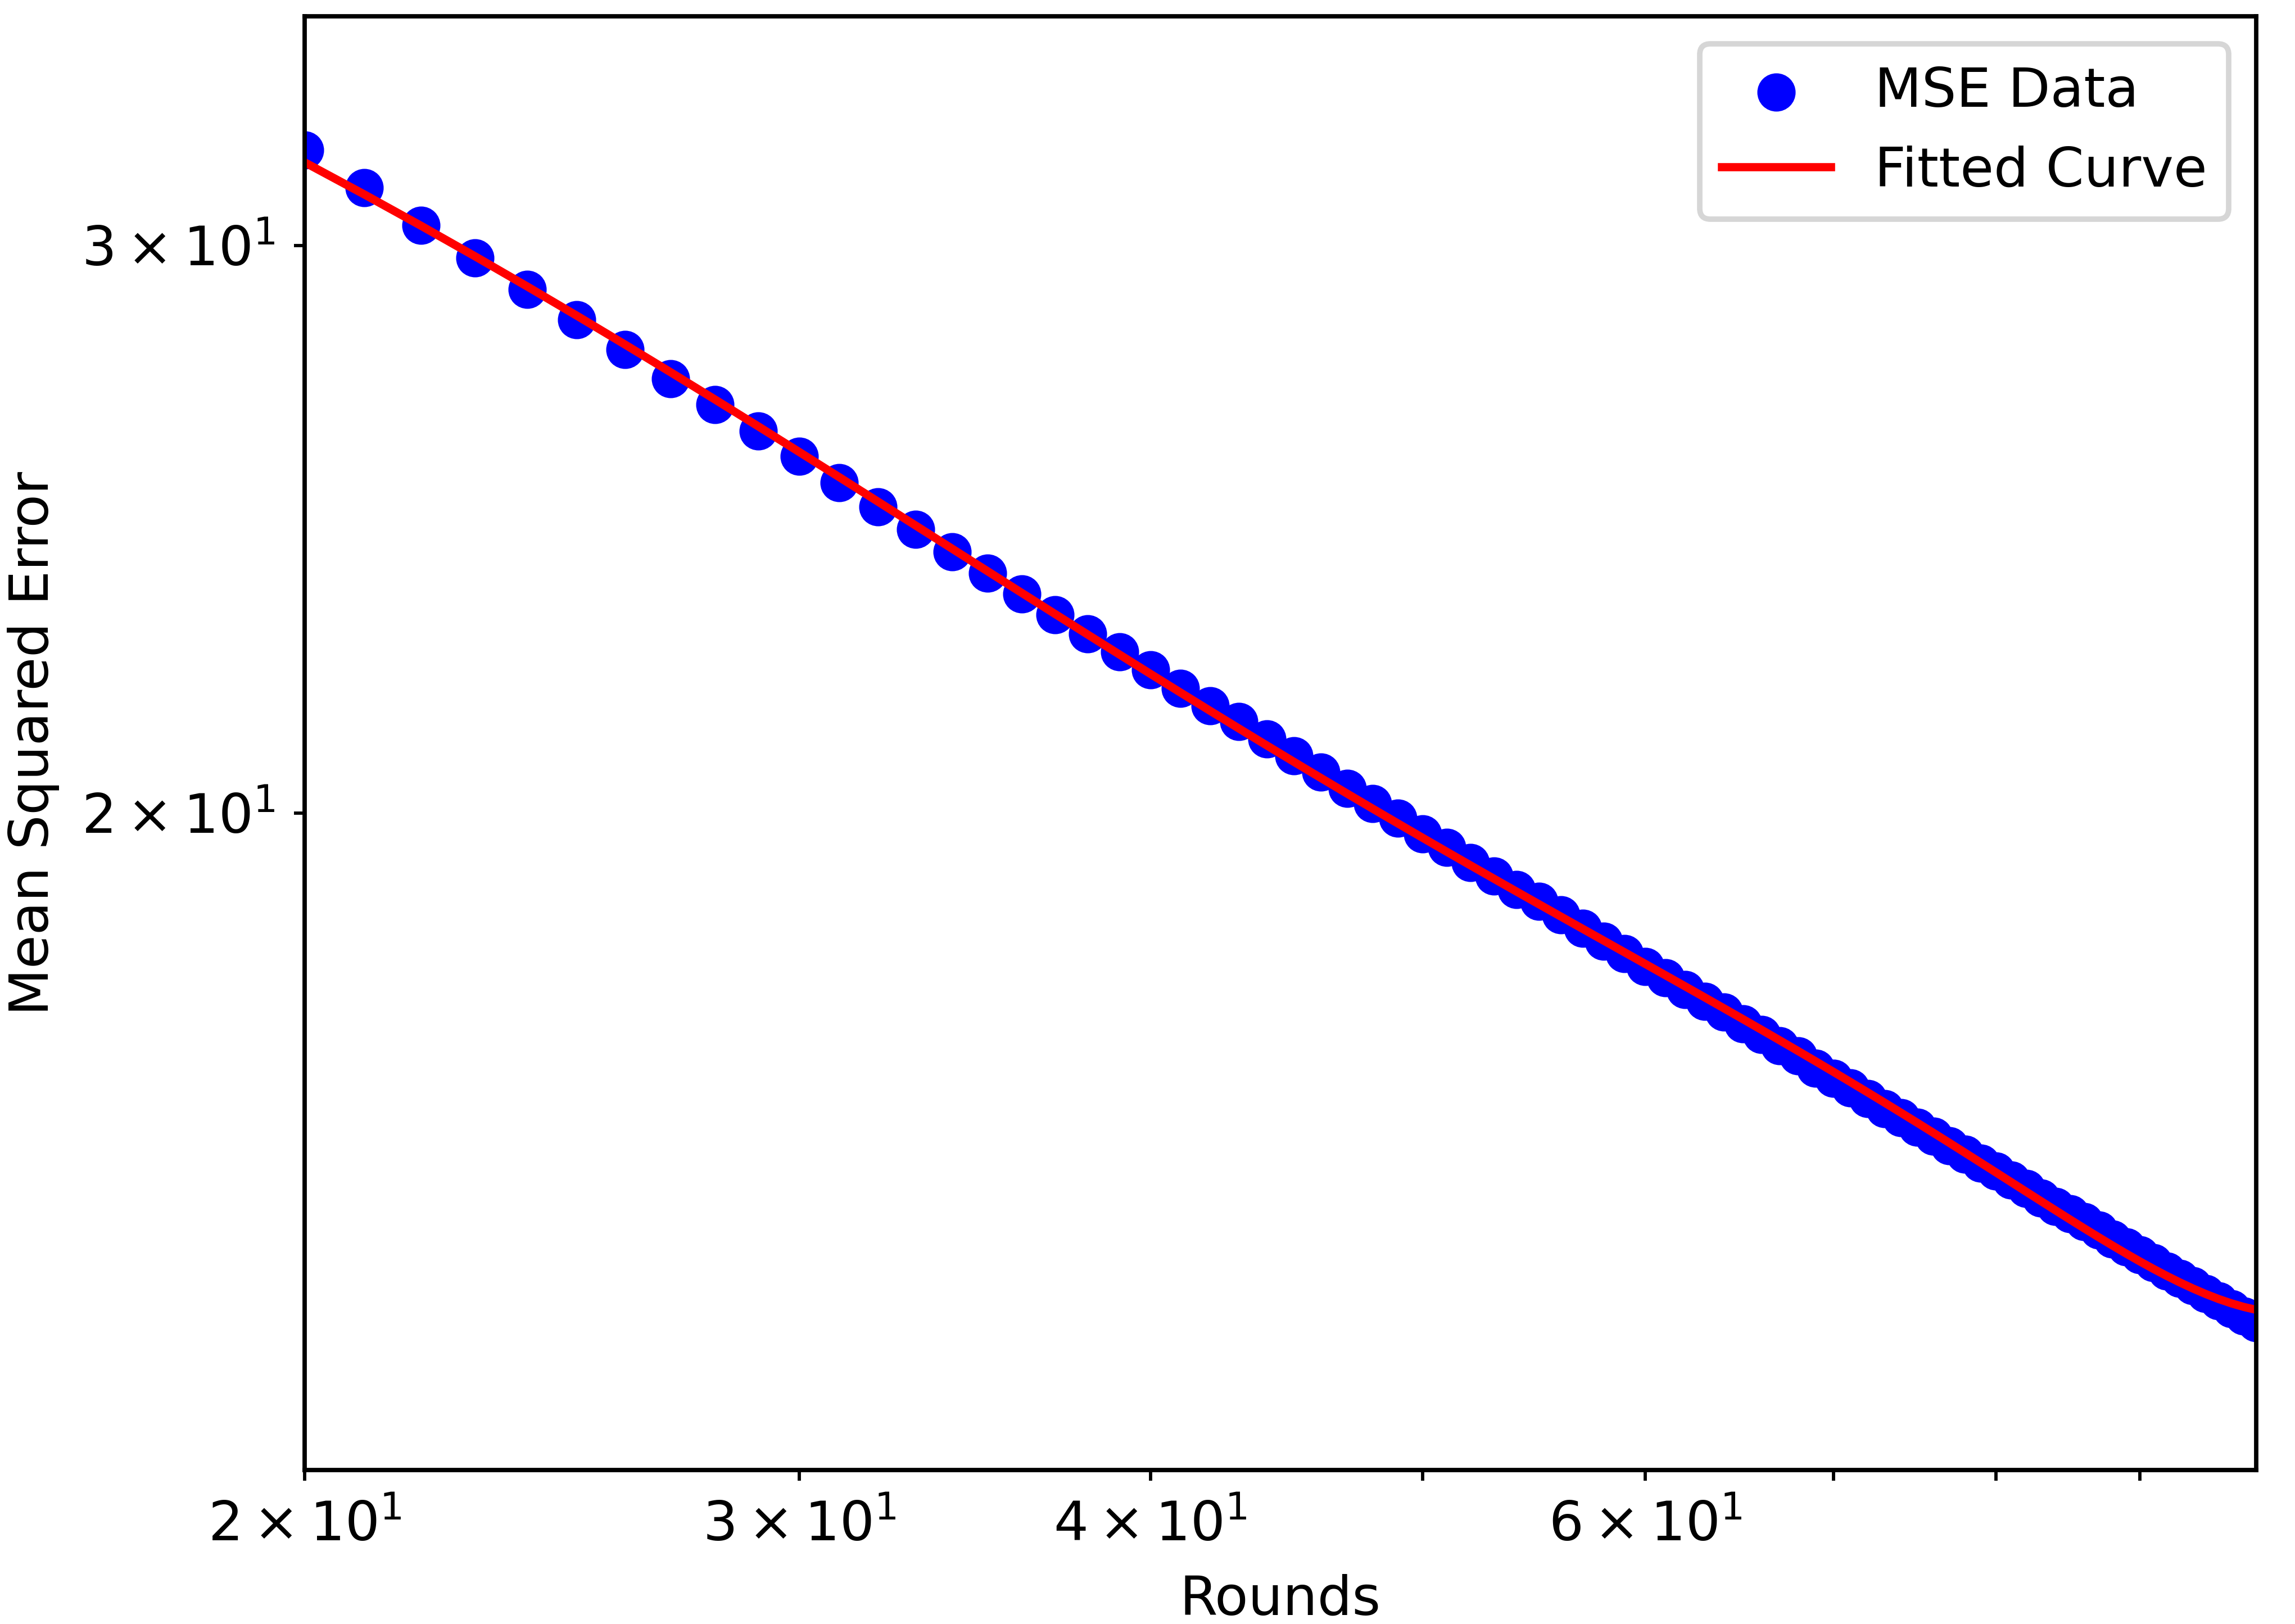
\includegraphics{figures/Simulation_outcomes/LollipopGraph/512_512/ATPPS/ATPPS_modelfitting_rounds_99_model_2.png}}
    \caption{(512, 512)-Lollipop graph - polynomial regression fit - ATPPS}
    \label{fig:atppslollipopgraphModelFit}
\end{figure}

\begin{figure}
    \centering
    \scalebox{0.8}{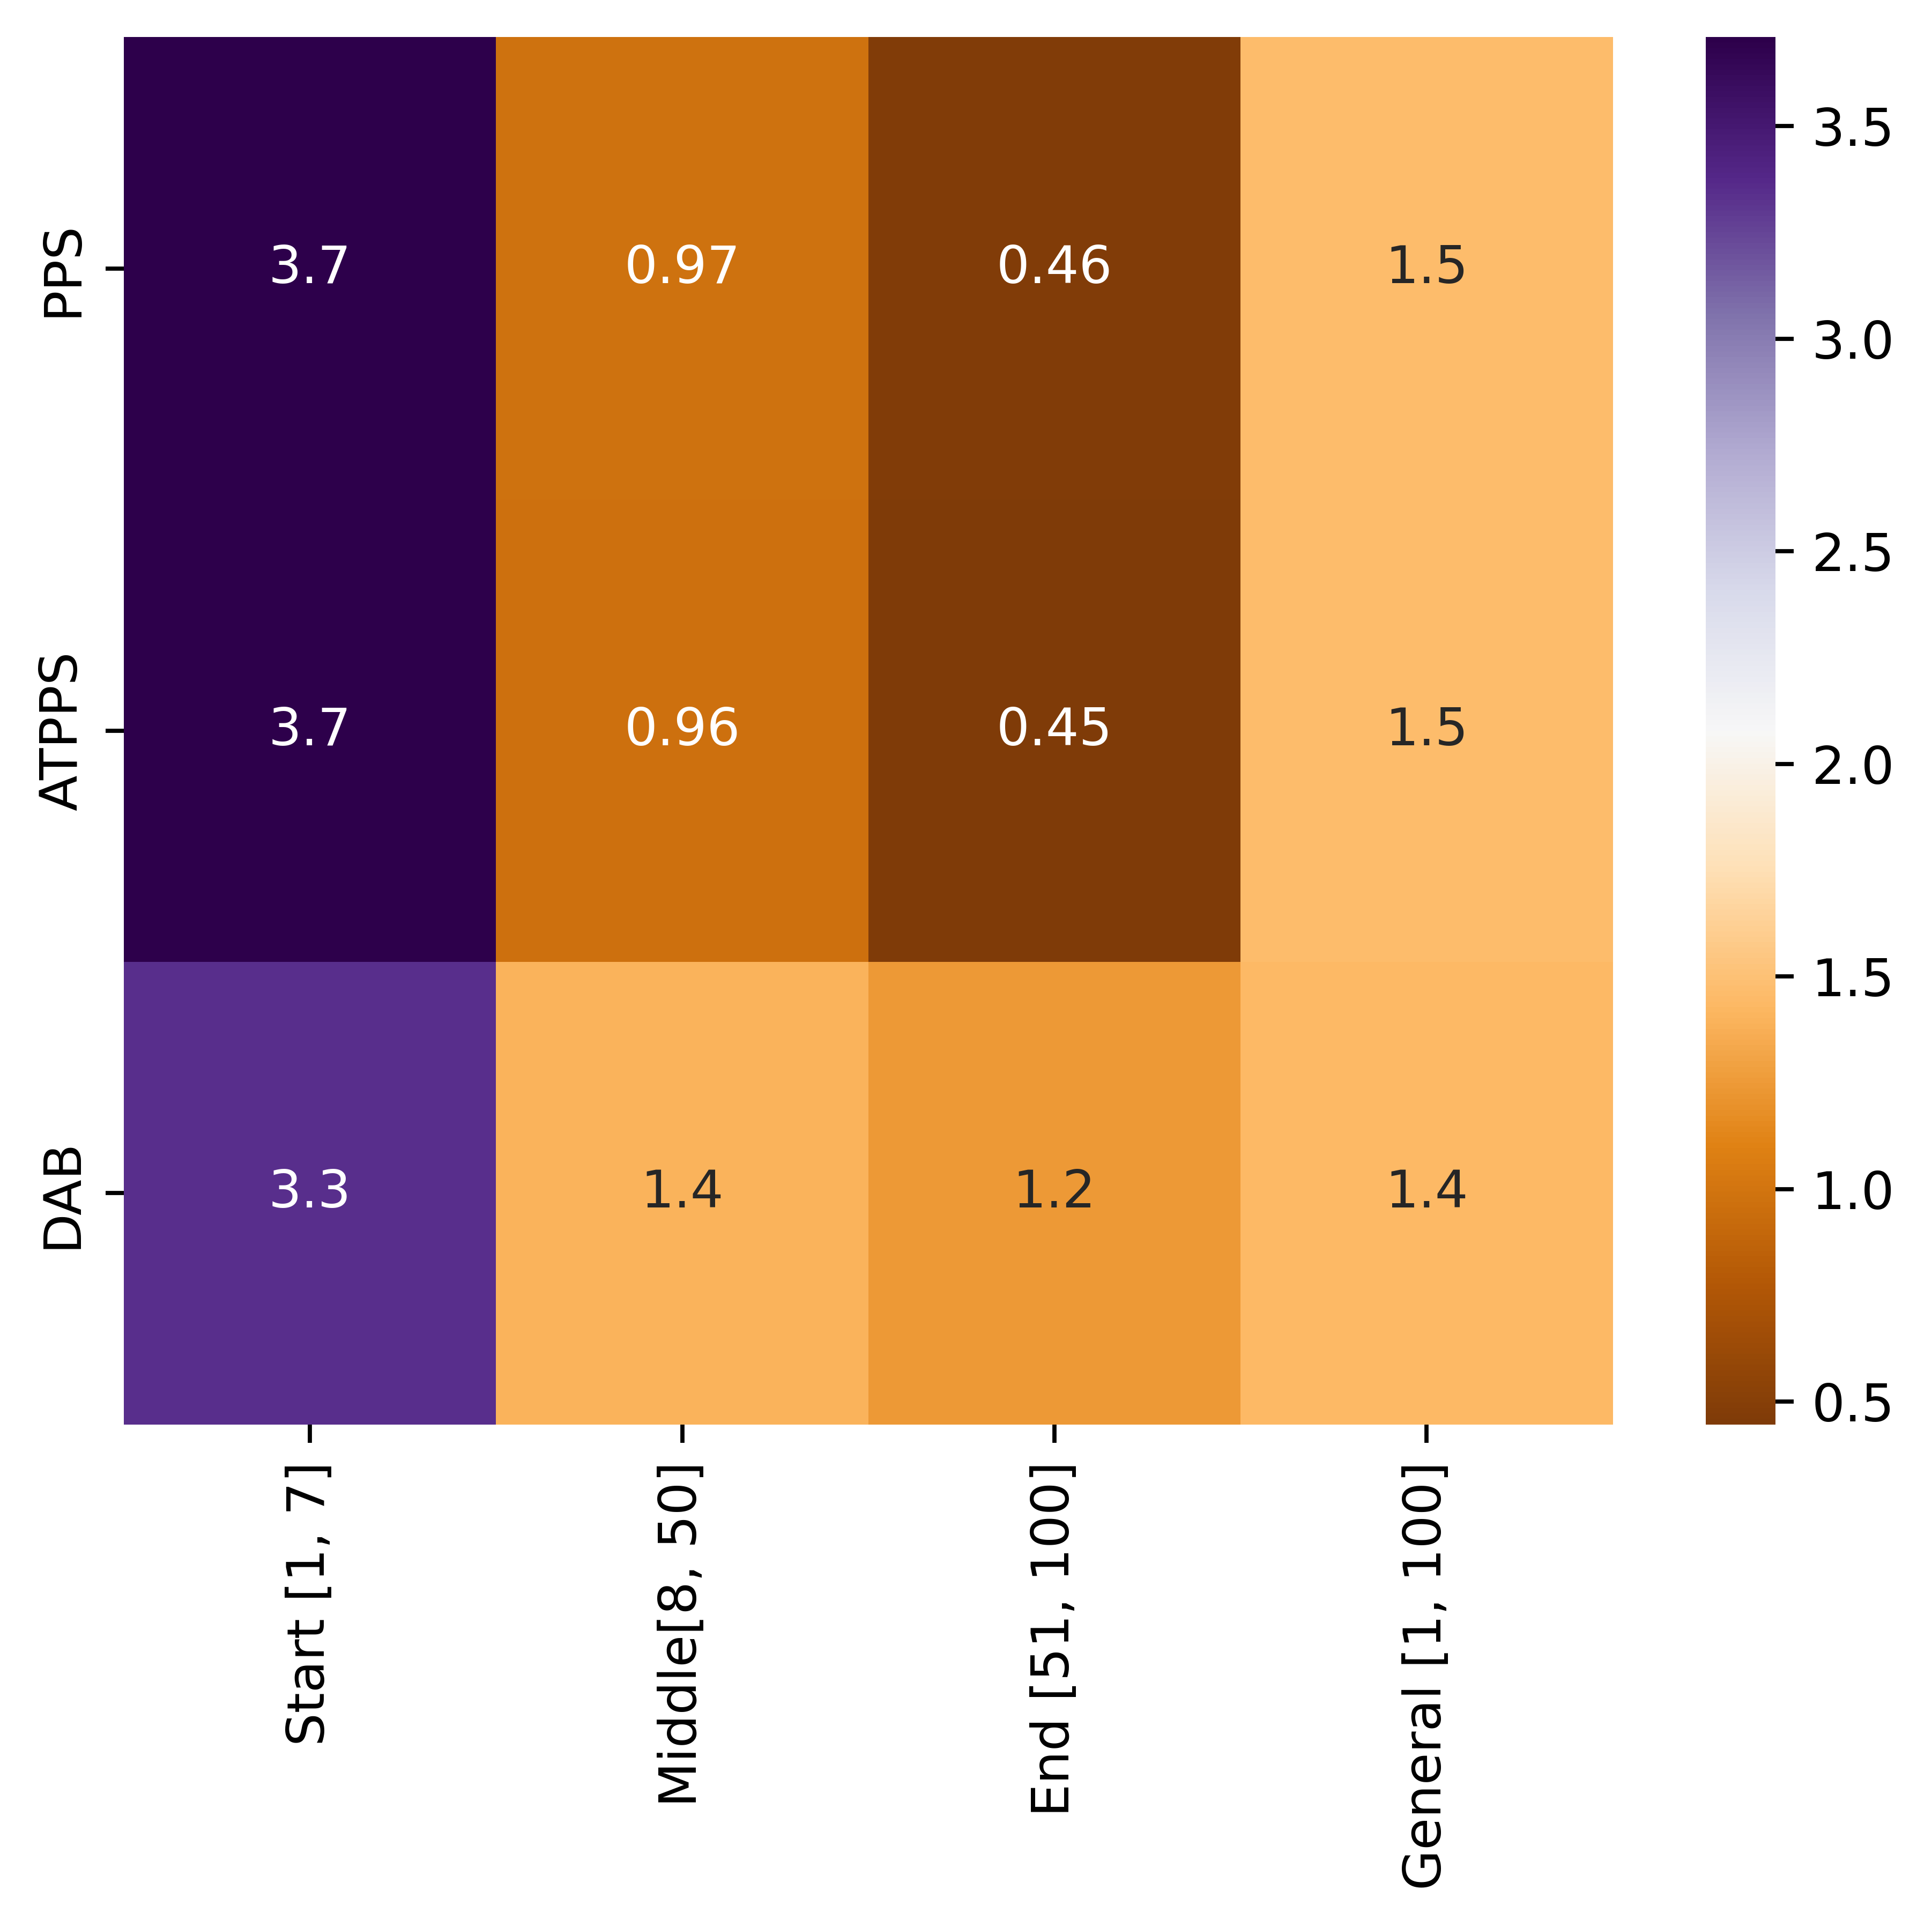
\includegraphics{figures/Simulation_outcomes/LollipopGraph/512_512/DAB_vs_PPS_vs_ATPPS_slopesheatmap_100rounds_log_log.png}}
    \caption{(512, 512)-Lollipop graph - heat map of slopes per region - log-log}
    \label{fig:lollipopslopes}
\end{figure}

To analyze the impact of the path size and clique size on the simulation results, additional simulations were conducted with varying proportions of nodes assigned to each region. In subsection \ref{subsec:128_896lollipop}, the number of nodes assigned to the clique is reduced to 128, which is one-fourth of the previous value of 512. Consequently, the path section now consists of 896 nodes. The total network size remains unchanged. This adjustment allows us to observe how a more dominant path section influences the load balancing behavior of the different algorithms. Similarly, in subsection \ref{subsec:896_128lollipop}, the simulations are performed with a reduced path size, assigning 896 nodes to the clique and only 128 nodes to the path. This configuration provides insight into how a more densely connected clique affects the overall performance of the algorithms.

\subsection{(128, 896)-Lollipop Graph}\label{subsec:128_896lollipop}
In the initial phase (the first 7 rounds) for the (128, 896)-Lollipop Graph $L_{128,896}$ the PPS and ATPPS start with a steep decline in MSE, both with a slope of -1.2, as shown in figure \ref{fig:128_896lollipopslopes}. DAB demonstrates a slightly slower initial convergence, with a slope of -0.86. Compared to the previous experiment, where the path size and clique sizes were equal, DAB's performance in the initial rounds has improved. The slope in this region in the previous experiment was -0.34 and improved to -0.86, which indicates a faster initial error reduction. In the middle region, rounds 8 to 50, the ATPPS shows a performance close to that of the PPS where both curves maintain a consistently steep slope. In the middle region, the PPS manages to increase its performance again slightly, recognisable by the fact that the slope has fallen by 0.1. The ATPPS manages to close the MSE discrepancy to the PPS in the end region. In this region, the ATPPS emits the largest drop in MSE. In the end phase the DAB shows a slightly shallower decline (-0.78) in MSE compared to earlier rounds. This could be attributed to the fact that once most of the load has propagated through the path, the balancing process along the clique slows. Both Push-Pull Sum variants continue to outperform DAB, achieving lower MSE values in fewer rounds due to their efficient clique-based load redistribution. Interestingly, PPS and ATPPS exhibit a slight divergence between rounds 10 and 90, before finally intersecting (or nearly so) around round 100. The PPS and ATPPS MSE data are very close to each other in round 100, suggesting that the ATPPS does not lead to an improved load balancing behavior. 

\begin{figure}[]
    \centering
    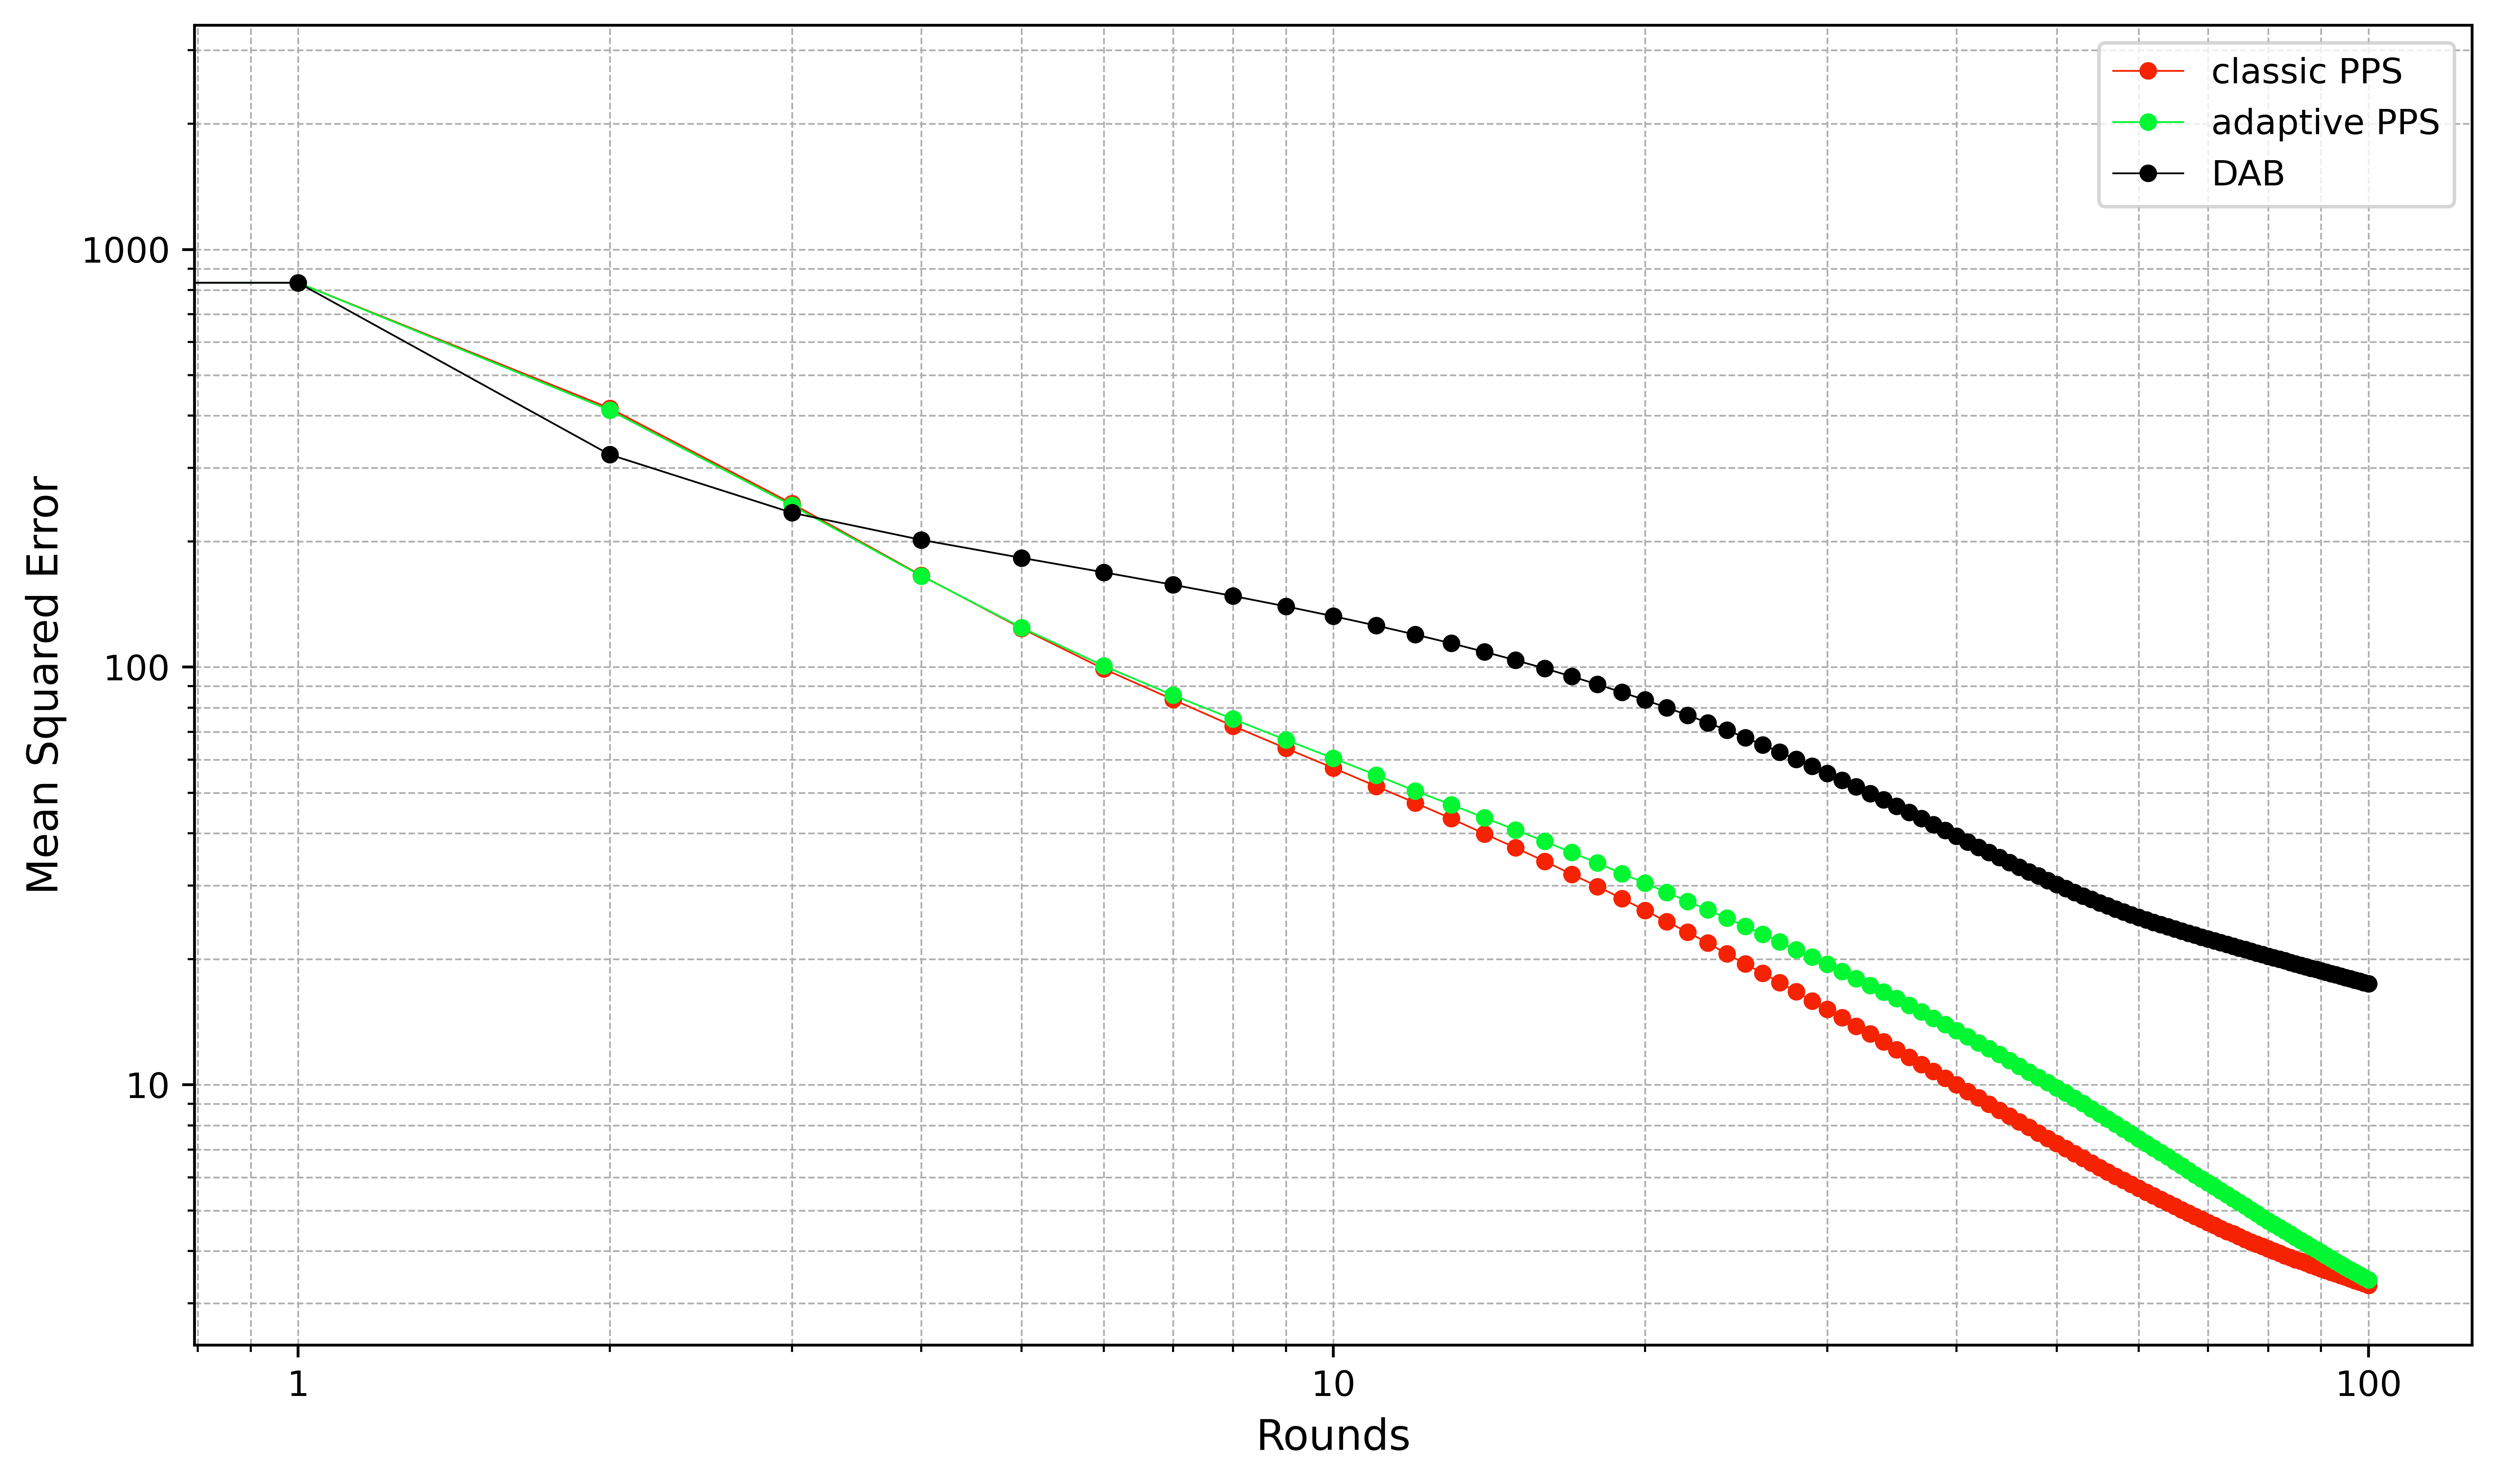
\includegraphics[width=\linewidth]{figures/Simulation_outcomes/LollipopGraph/128_896/DAB_vs_PPS_LG_r100_n1024_averaged_loglog.png}
    \caption{(128, 896)-Lollipop graph - mean squared error per rounds - log-log}
    \label{fig:128_896lollipopgraphMSEperRoundLogLog}
\end{figure}

The MSE data of all three load balancing algorithms were fitted to polynomial regression models. The MSE data for DAB and ATPPS were best approximated by polynomials of degree 4, while the PPS MSE data exhibited slightly more complex behavior, following a polynomial of degree 5. The fitted model for the DAB MSE data follows the equation: 
\begin{align}
    MSE_r=3.46\times 10^{-6}r^{4}-1.12\times 10^{-3}r^{3}+0.14r^{2}-7.69r+190.78    
\end{align}
(figure \ref{fig:dab_128x896lollipopgraphModelFit}). For ATPPS, the polynomial fit is given by:
\begin{align}
    MSE_r=1.59\times 10^{-6}r^{4}-4.74\times 10^{-4}r^{3}+0.054r^{2}-2.94r+70.59    
\end{align}
(figure \ref{fig:pps_128x896lollipopgraphModelFit}). The PPS MSE data, which required a higher-degree polynomial (degree 5), follows the equation:
\begin{align}
    MSE_r=-3.72\times10^{-8}r^{5}+1.31\times 10^{-5}r^{4}-1.85\times 10^{-3}r^{3}+0.13r^{2}-4.96r+84.91    
\end{align}
(figure \ref{fig:atpps_128x896lollipopgraphModelFit}).

\begin{figure}[]
    \centering
    \scalebox{0.8}{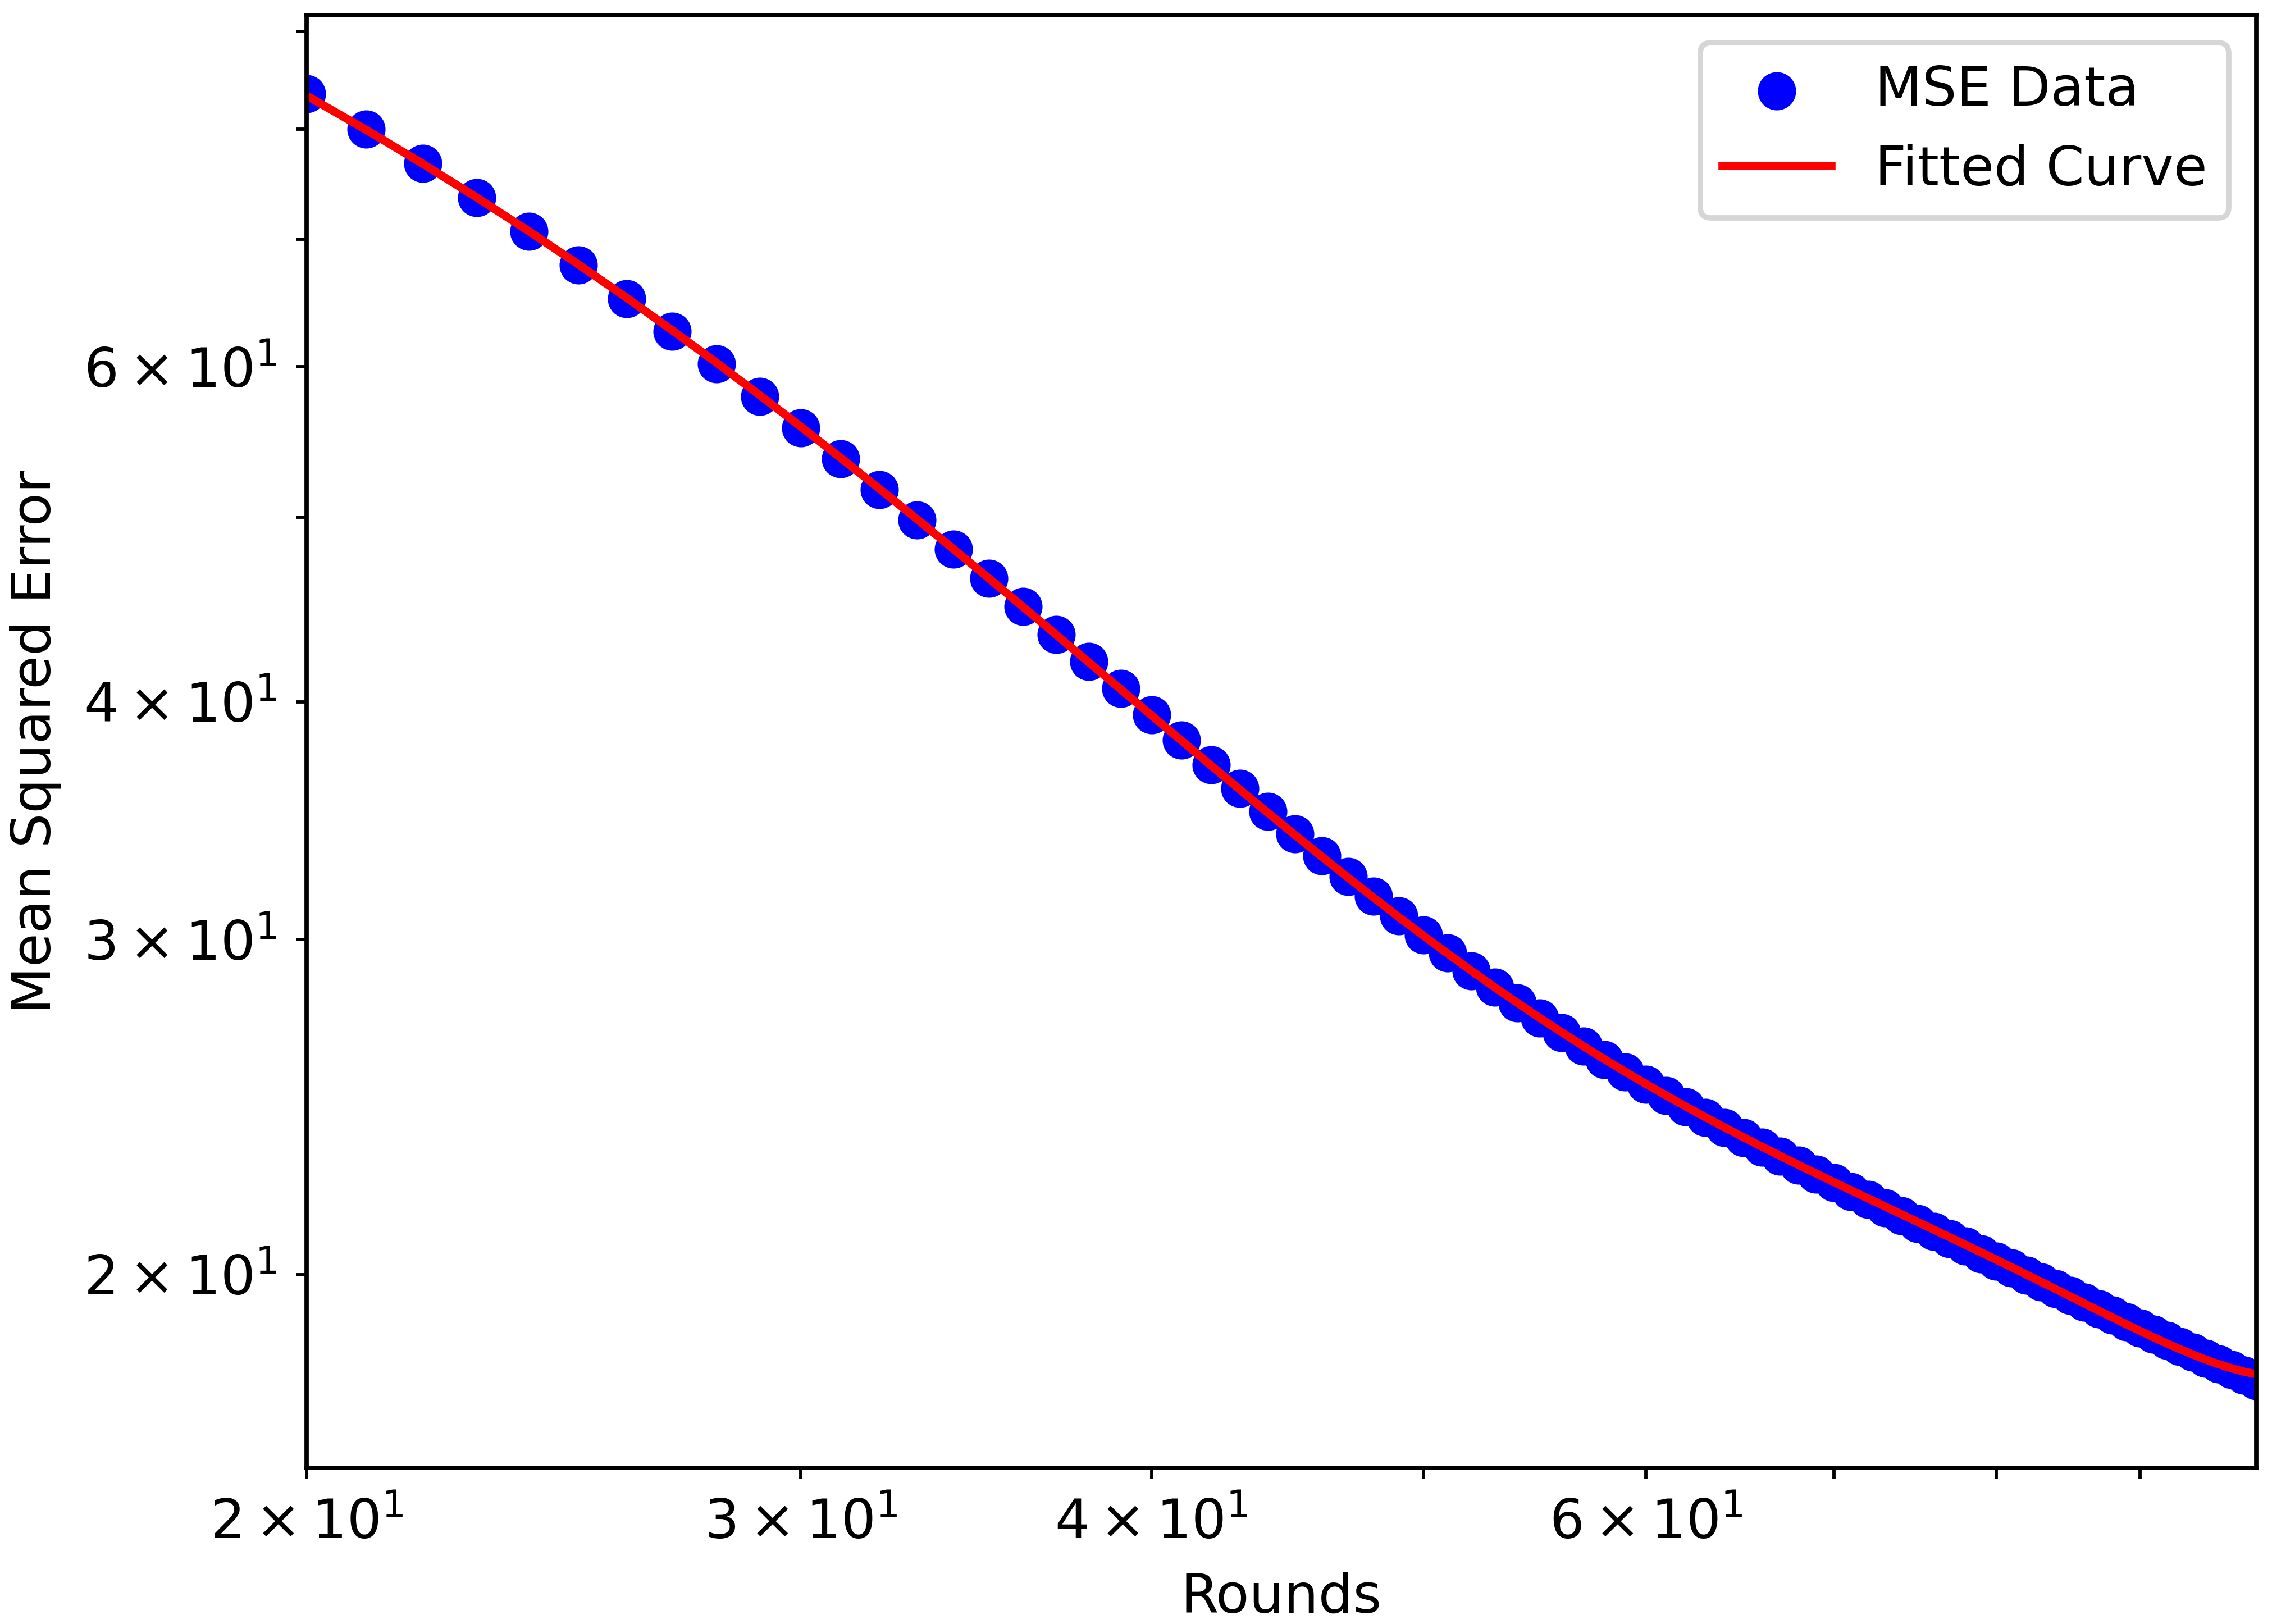
\includegraphics{figures/Simulation_outcomes/LollipopGraph/128_896/DAB/DAB_modelfitting_rounds_99_model_2.png}}
    \caption{(128, 896)-Lollipop graph - polynomial regression fit - DAB}
    \label{fig:dab_128x896lollipopgraphModelFit}
\end{figure}

\begin{figure}[]
    \centering
    \scalebox{0.8}{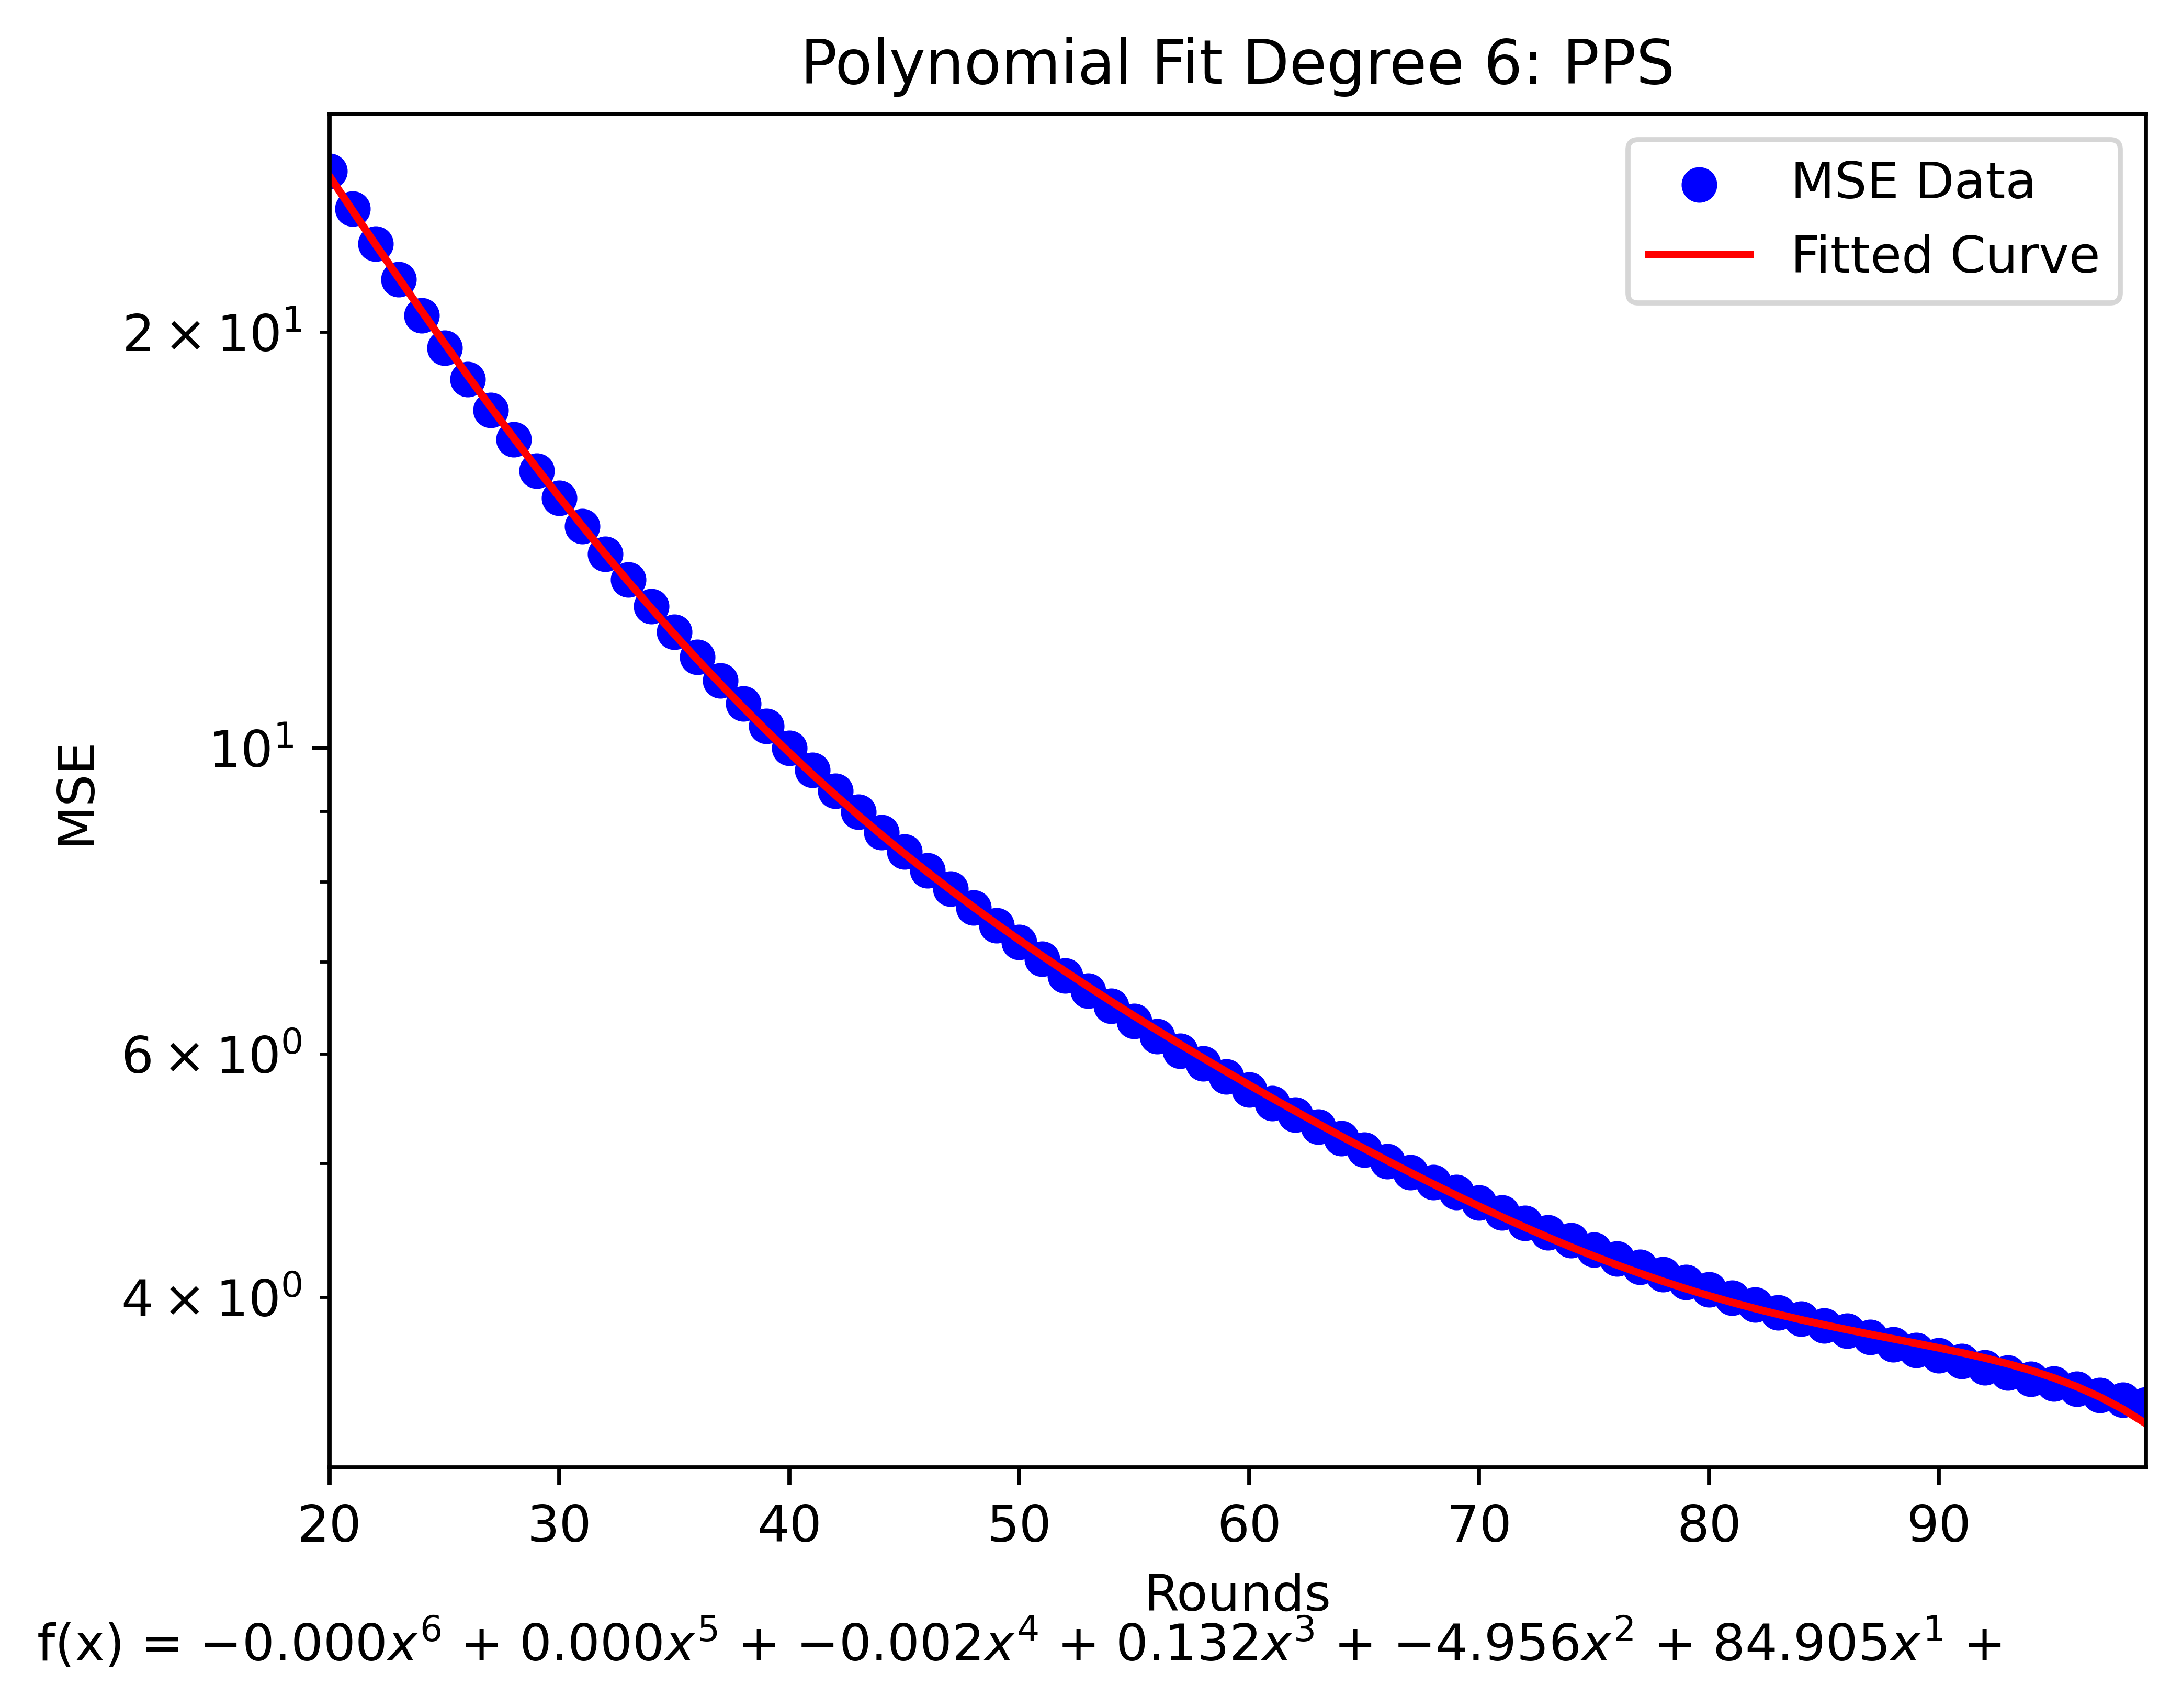
\includegraphics{figures/Simulation_outcomes/LollipopGraph/128_896/PPS/PPS_modelfitting_rounds_99_model_2.png}}
    \caption{(128, 896)-Lollipop graph - polynomial regression fit - PPS}
    \label{fig:pps_128x896lollipopgraphModelFit}
\end{figure}

\begin{figure}[]
    \centering
    \scalebox{0.8}{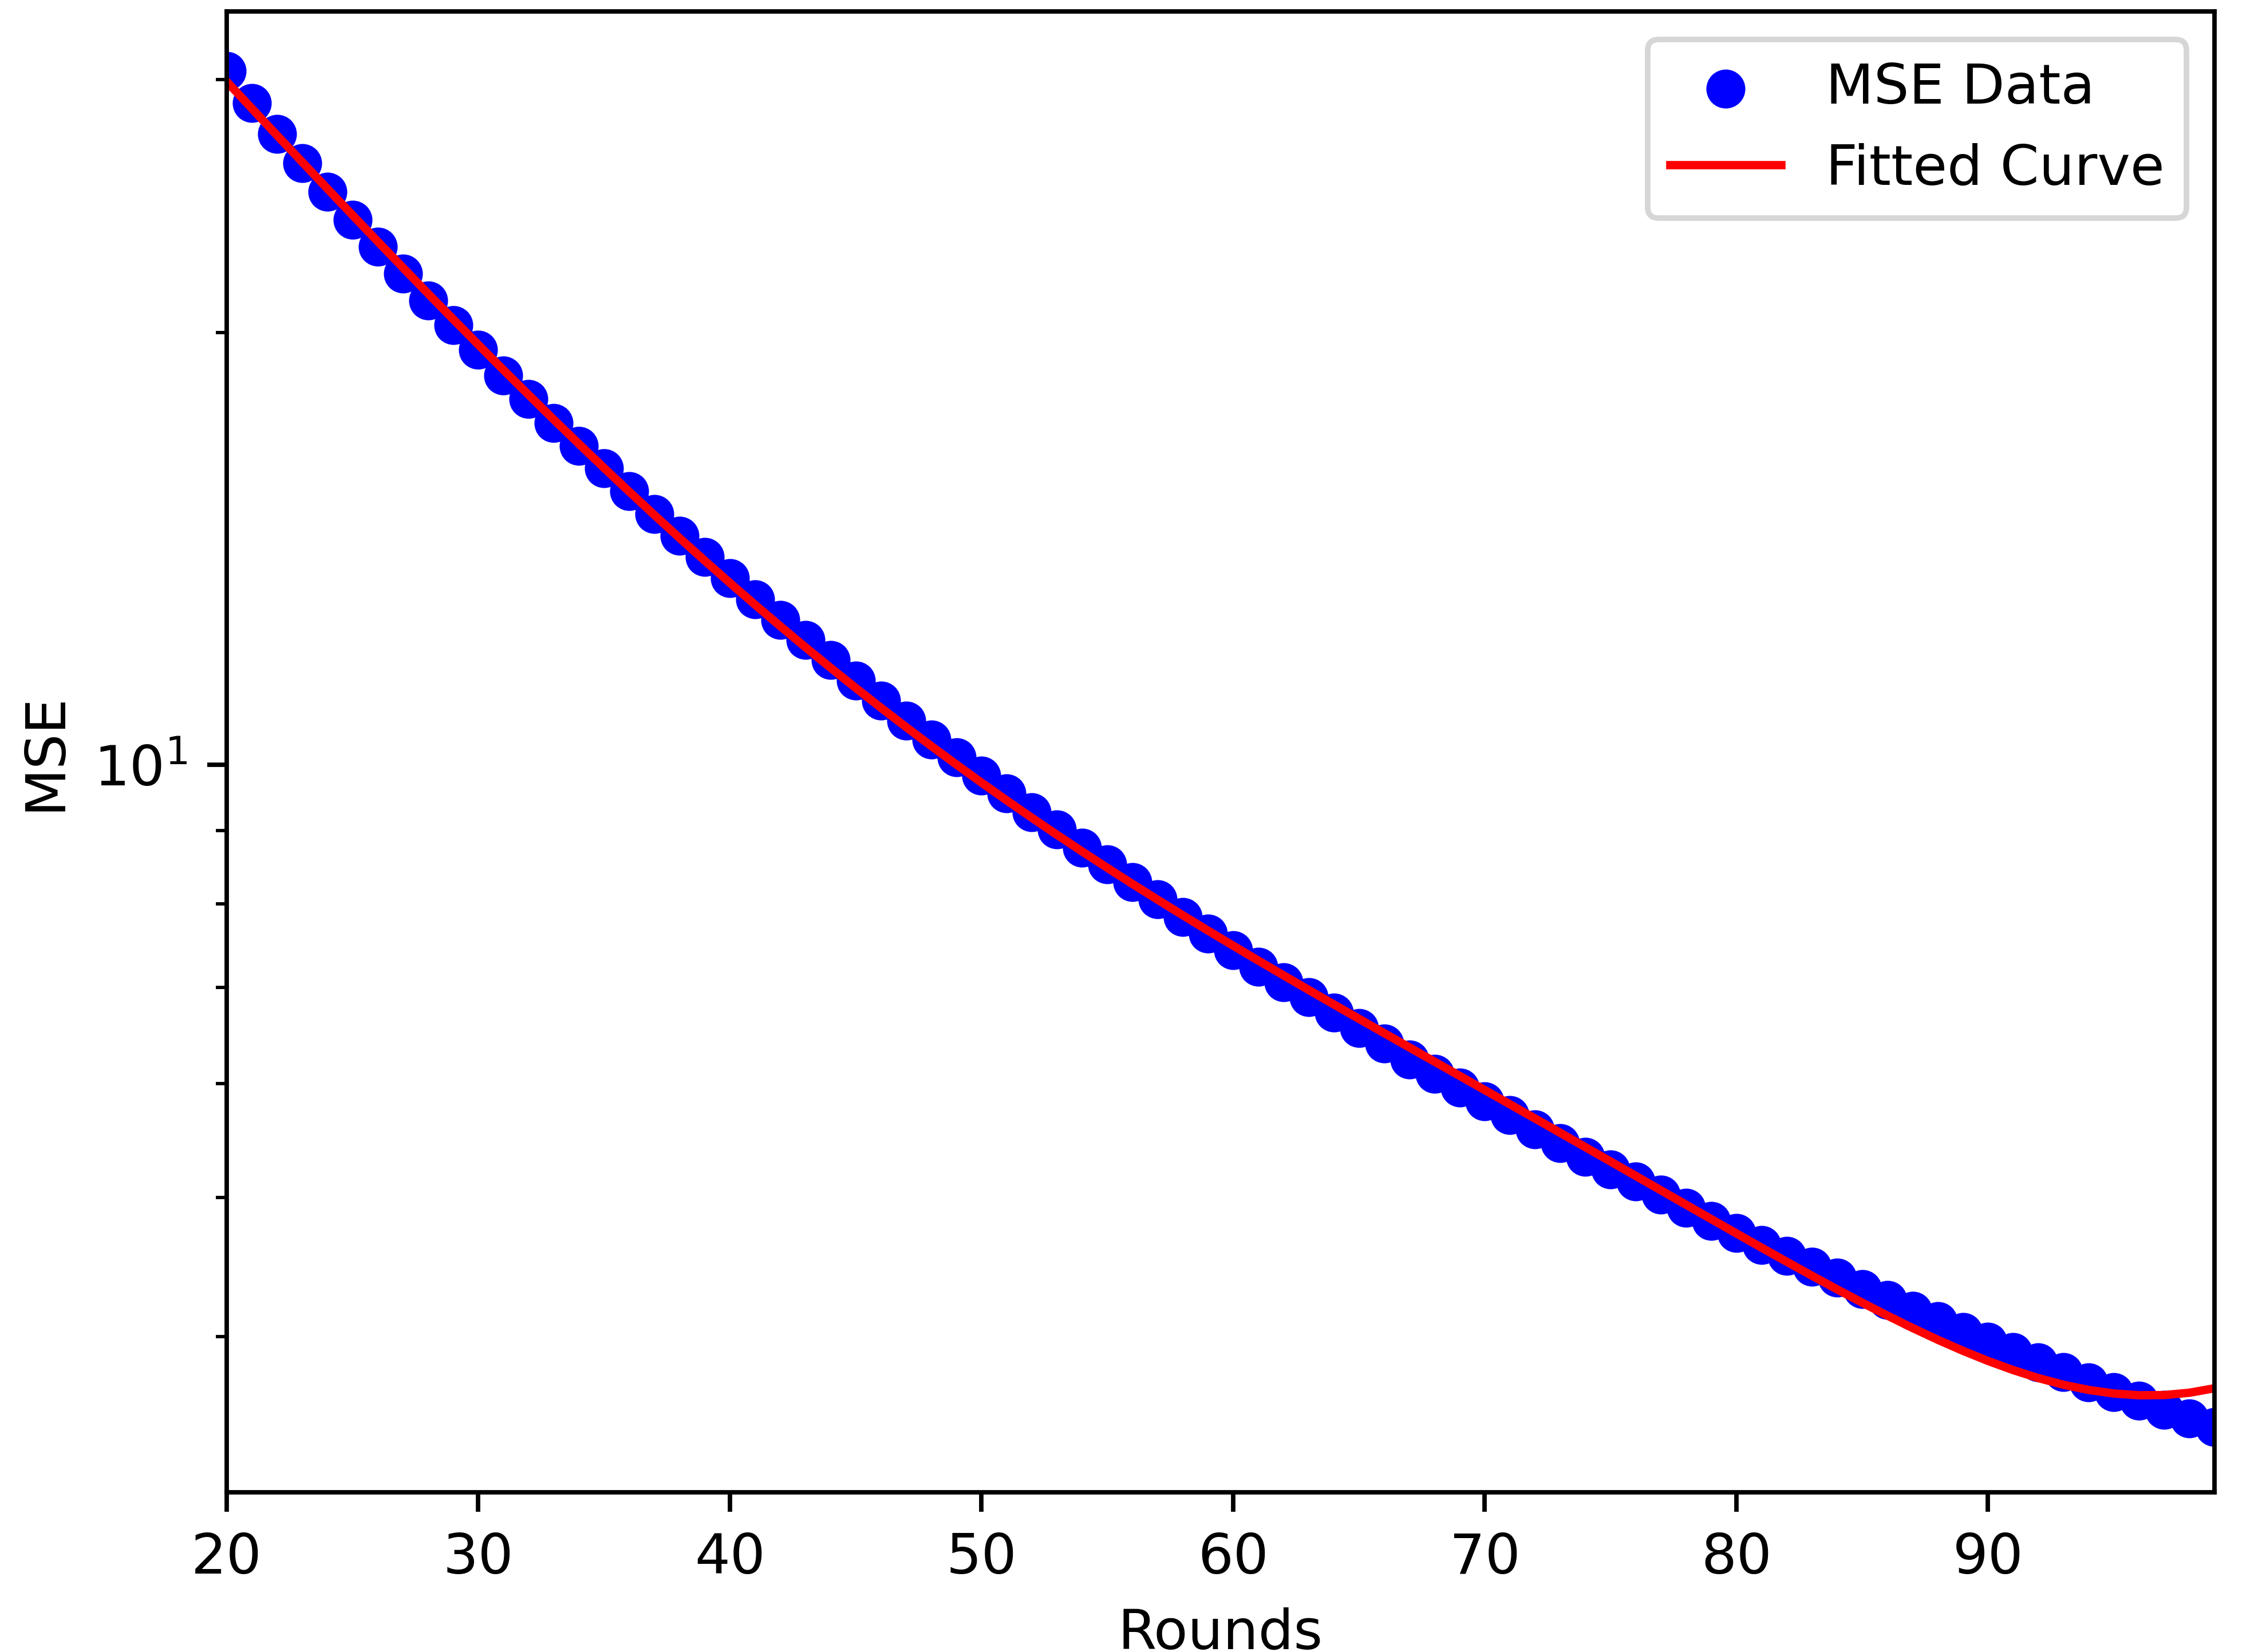
\includegraphics{figures/Simulation_outcomes/LollipopGraph/128_896/ATPPS/ATPPS_modelfitting_rounds_99_model_2.png}}
    \caption{(128, 896)-Lollipop graph - polynomial regression fit - ATPPS}
    \label{fig:atpps_128x896lollipopgraphModelFit}
\end{figure}

\begin{figure}
    \centering
    \scalebox{0.8}{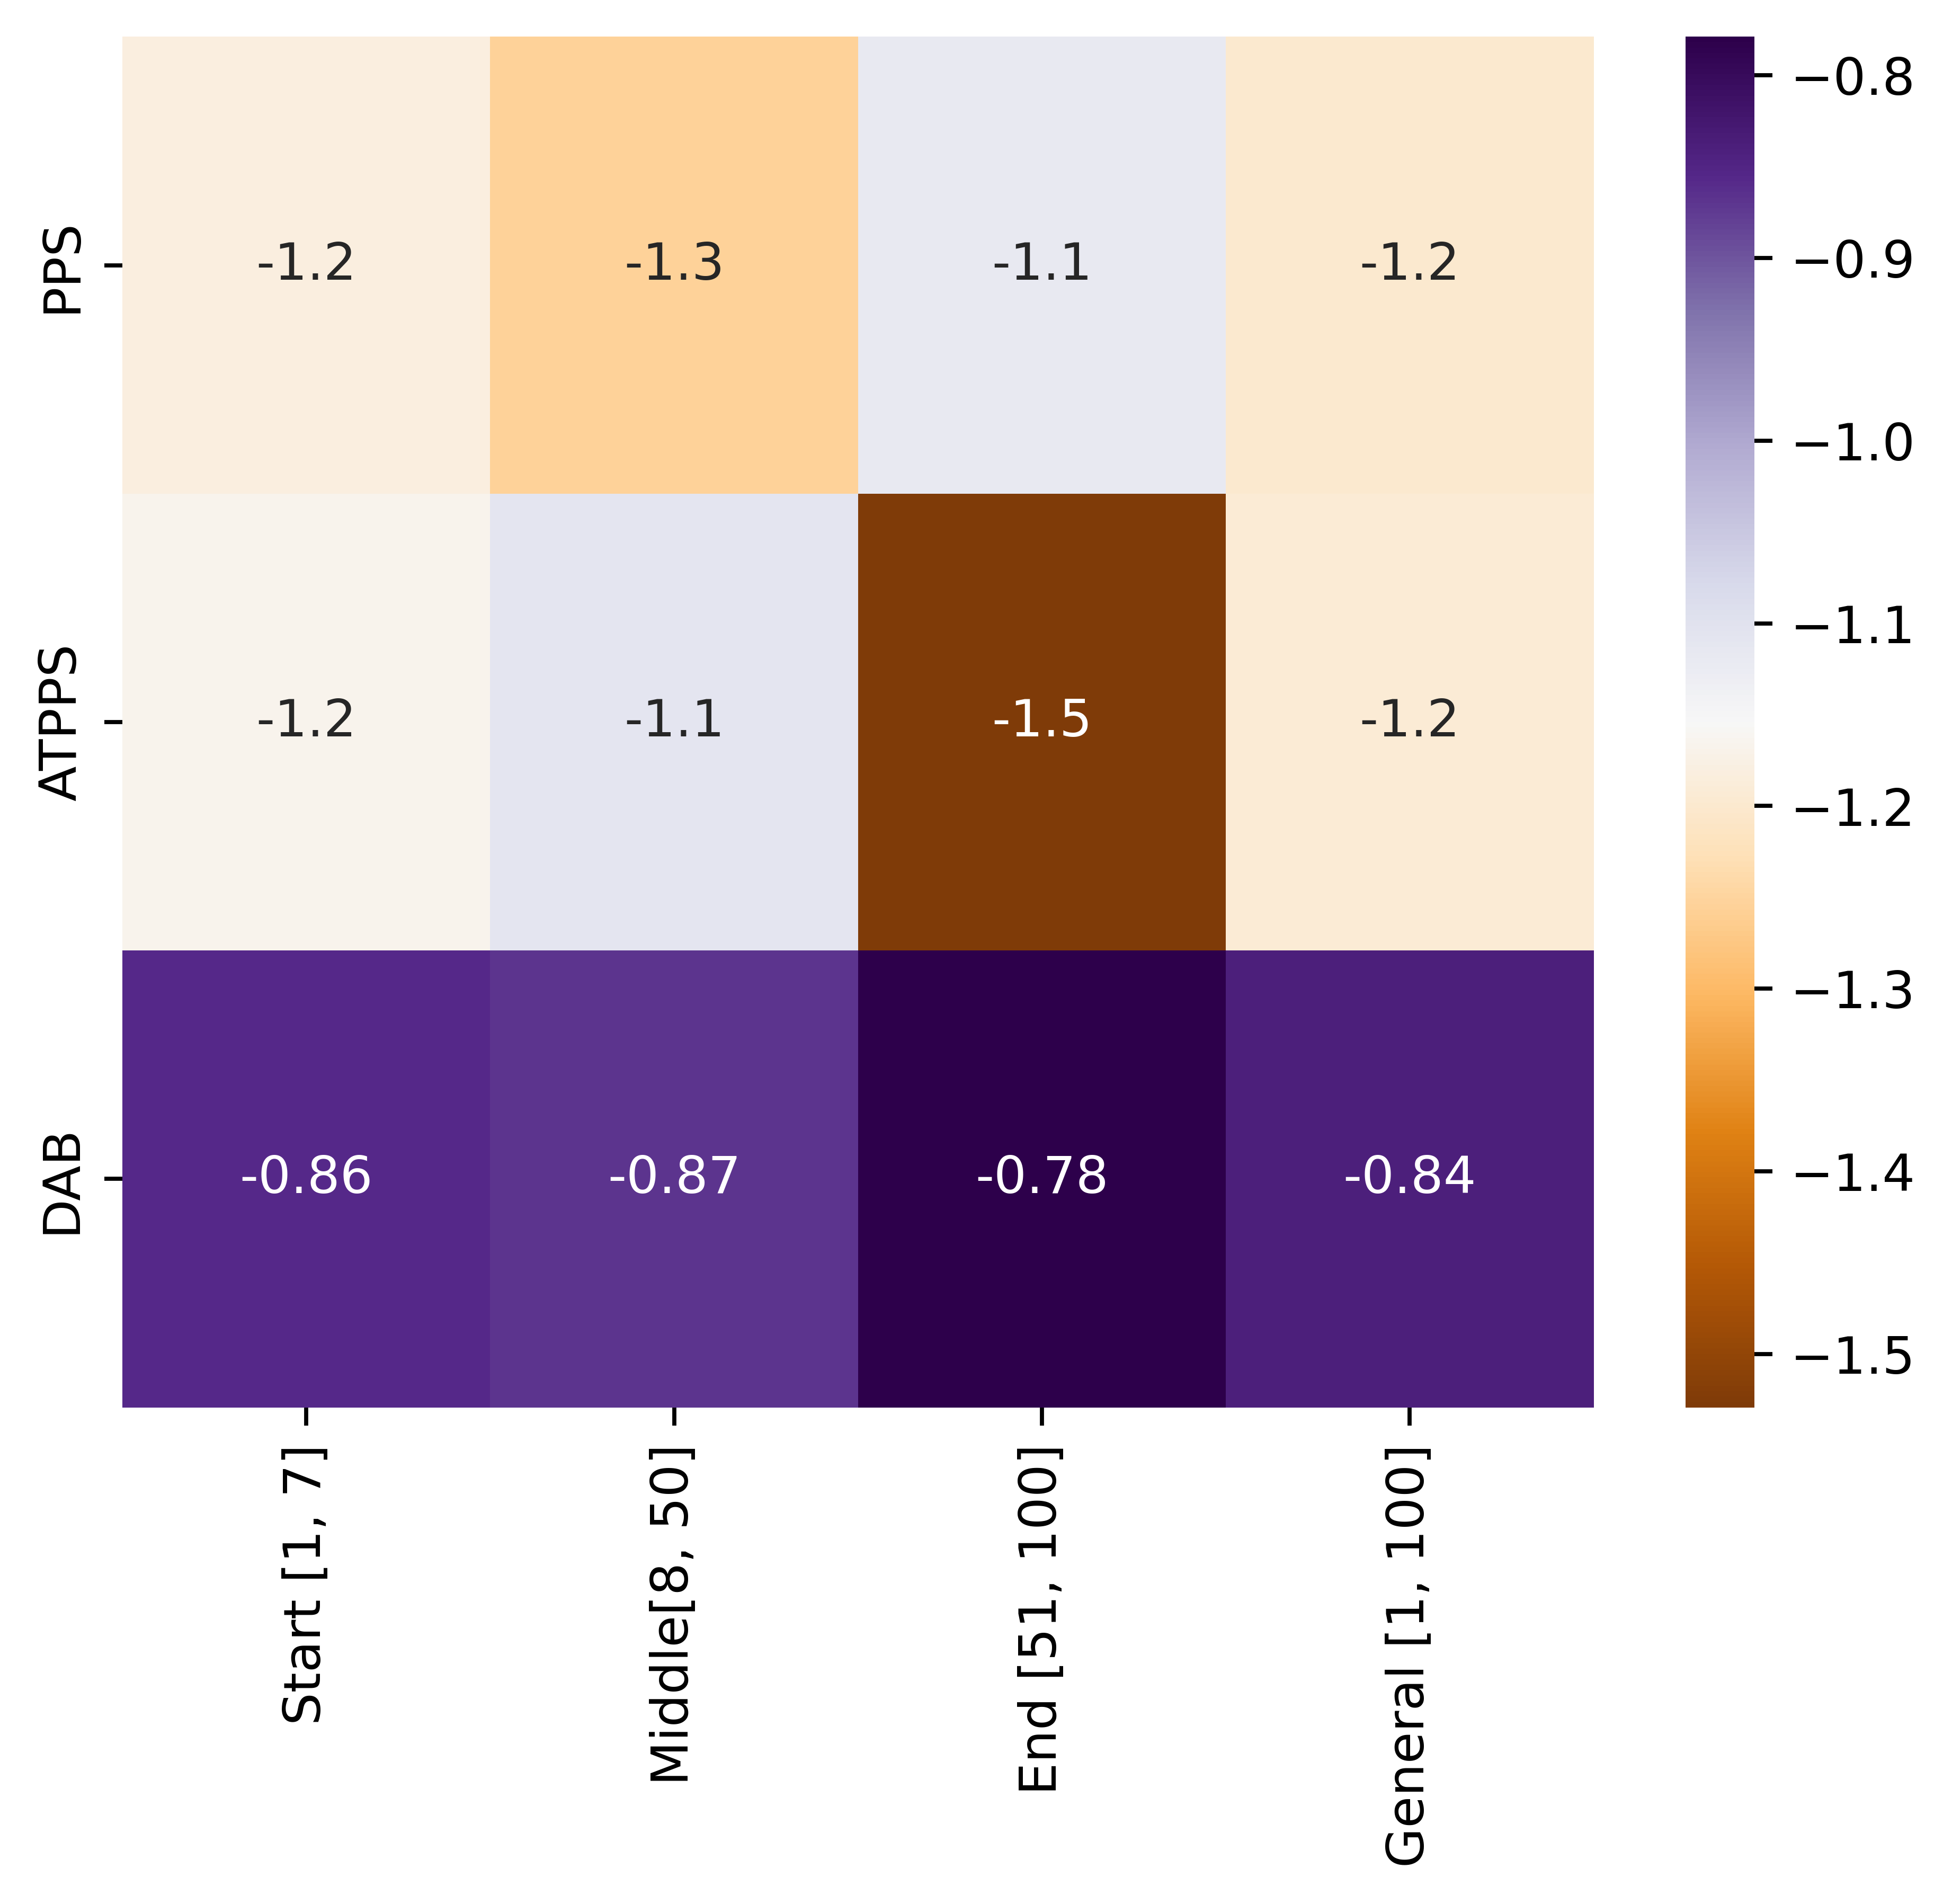
\includegraphics{figures/Simulation_outcomes/LollipopGraph/128_896/DAB_vs_PPS_vs_ATPPS_slopesheatmap_100rounds_log_log.png}}
    \caption{(128, 896)-Lollipop graph - heat map of slopes per region - log-log}
    \label{fig:128_896lollipopslopes}
\end{figure}

\subsection{(896, 128)-Lollipop Graph}\label{subsec:896_128lollipop}
As more nodes are assigned to the clique and fewer to the Path graph in $L_{896,128}$ compared to $L_{512,512}$, the performance gap between the Push-Pull Sum-based algorithms and the DAB becomes more pronounced, as shown in figure \ref{fig:896_128lollipopgraphMSEperRoundLogLog}. This is also reflected in the log-log slopes. In the start region, the Push-Pull Sum-based algorithms balance the network more quickly in $L_{896,128}$, achieving slopes of -2, compared to -1.3 in $L_{512,512}$ (figure \ref{fig:896x128lollipopslopes}). In the middle and end region, the slopes are almost quartered compared to the start region. The DAB achieves consistently low slopes: -0.08 in the start region, -0.1 in the middle region and -0.11 in the end region. The overall MSE is also lower for $L_{896,128}$, with the ATPPS reducing the error to 3.27 and the PPS to 3.59. In contrast, the MSE values for the $L_{512,512}$ graph are higher after 100 rounds, where ATPPS achieved a value of 13.83 and the PPS achieved a value of 14.71. Despite this, no significant advantage of the ATPPS over the PPS is observed. The DAB, however, struggles to reduce the error, with a substantial difference in MSE values after 100 rounds. In $L_{512,512}$, the DAB reaches an MSE of 108.90, while in $L_{896,128}$, the MSE increases to 542.09 - almost five times higher.

The best-fit polynomials for the MSE data of the load balancing algorithms are of degree 3 for the DAB and degree 4 for the Push-Pull Sum-based algorithms. The polynomial for the DAB MSE data is expressed as:
\begin{align}
    MSE_r=-1.93\times 10^{-4}r^{3}+0.05r^{2}-5.33r+745.95    
\end{align}
(figure \ref{fig:dab_896x128lollipopgraphModelFit}). For the PPS, the polynomial is: 
\begin{align}
    MSE_r=2.00\times 10^{-7}r^{4}-6.01\times 10^{-5}r^{3}+6.95\times 10^{-3}r^{2}-0.39r+13.44
\end{align}
(figure \ref{fig:pps_896x128lollipopgraphModelFit}) and for the ATPPS, is:
\begin{align}
    MSE_r=2.28\times 10^{-7}r^{4}-6.77\times 10^{-5}r^{3}+7.68\times 10^{-3}r^{2}-0.42r+13.62    
\end{align}
(figure \ref{fig:atpps_896x128lollipopgraphModelFit}).

\begin{figure}[!ht]
    \centering
        \subfloat[]{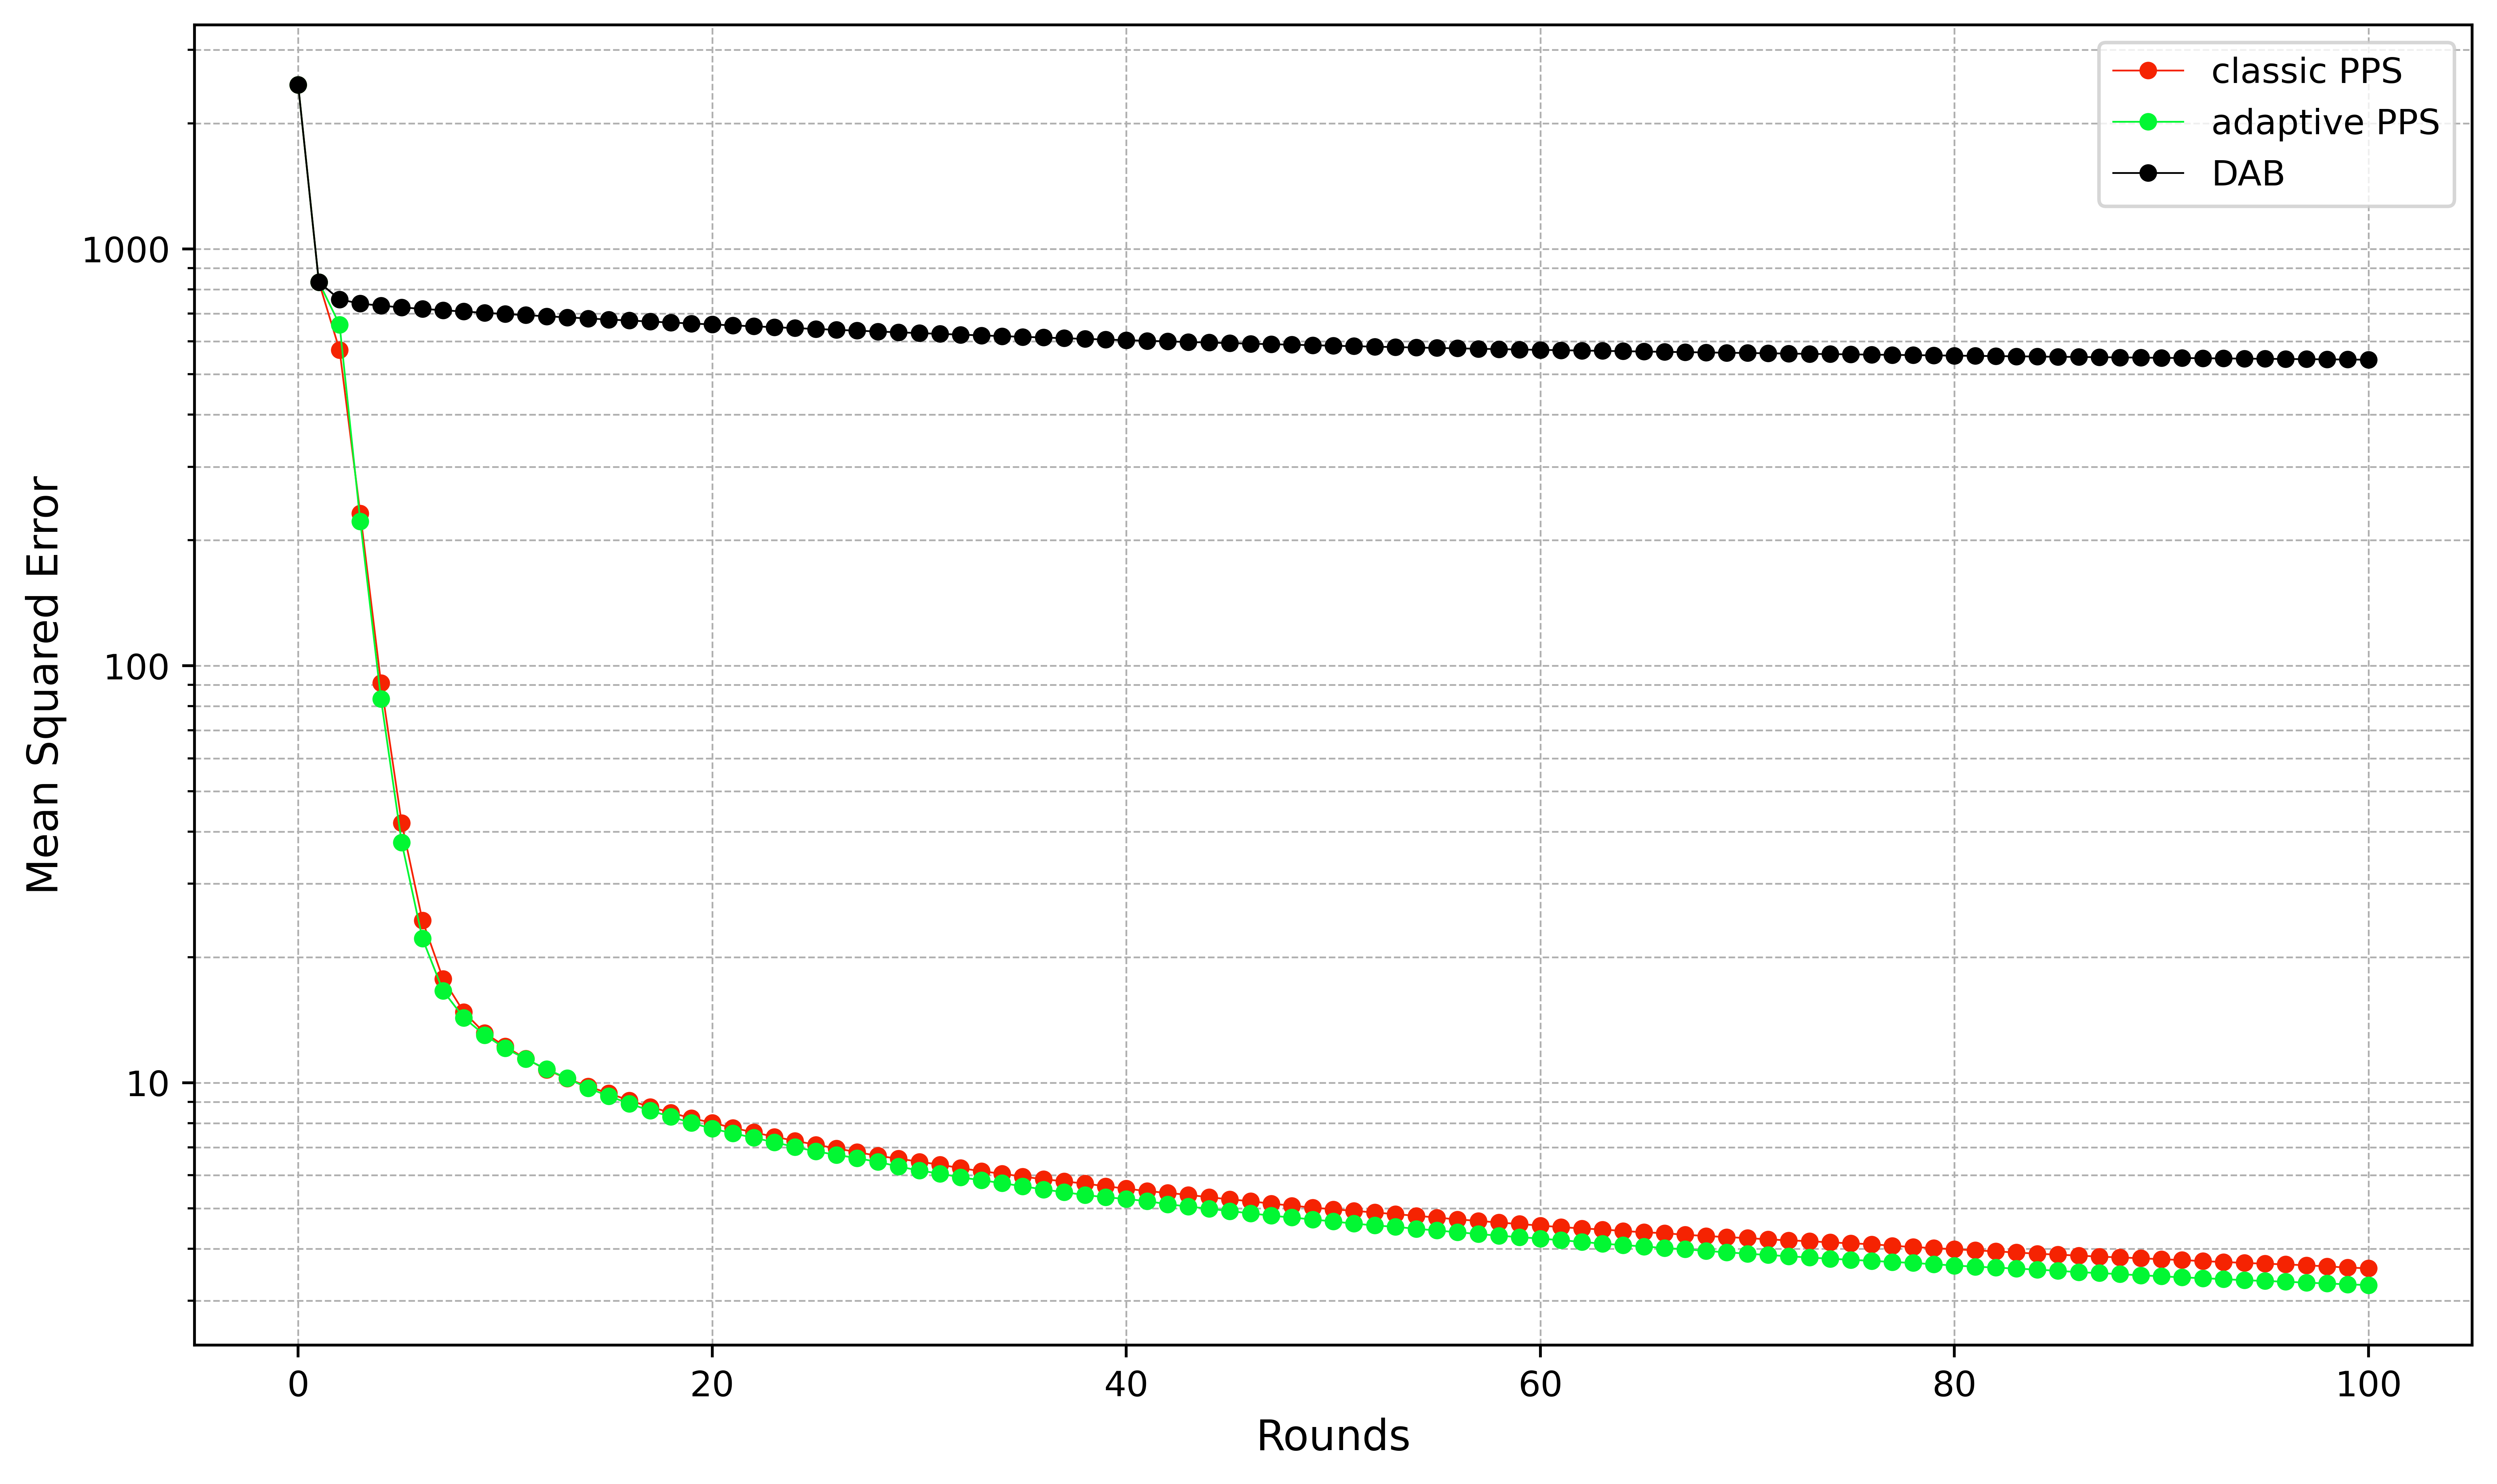
\includegraphics[width=0.49\linewidth]{figures/Simulation_outcomes/LollipopGraph/896_128/DAB_vs_PPS_LG_r100_n1024_averaged_log.png}}
    \hfil
        \subfloat[]{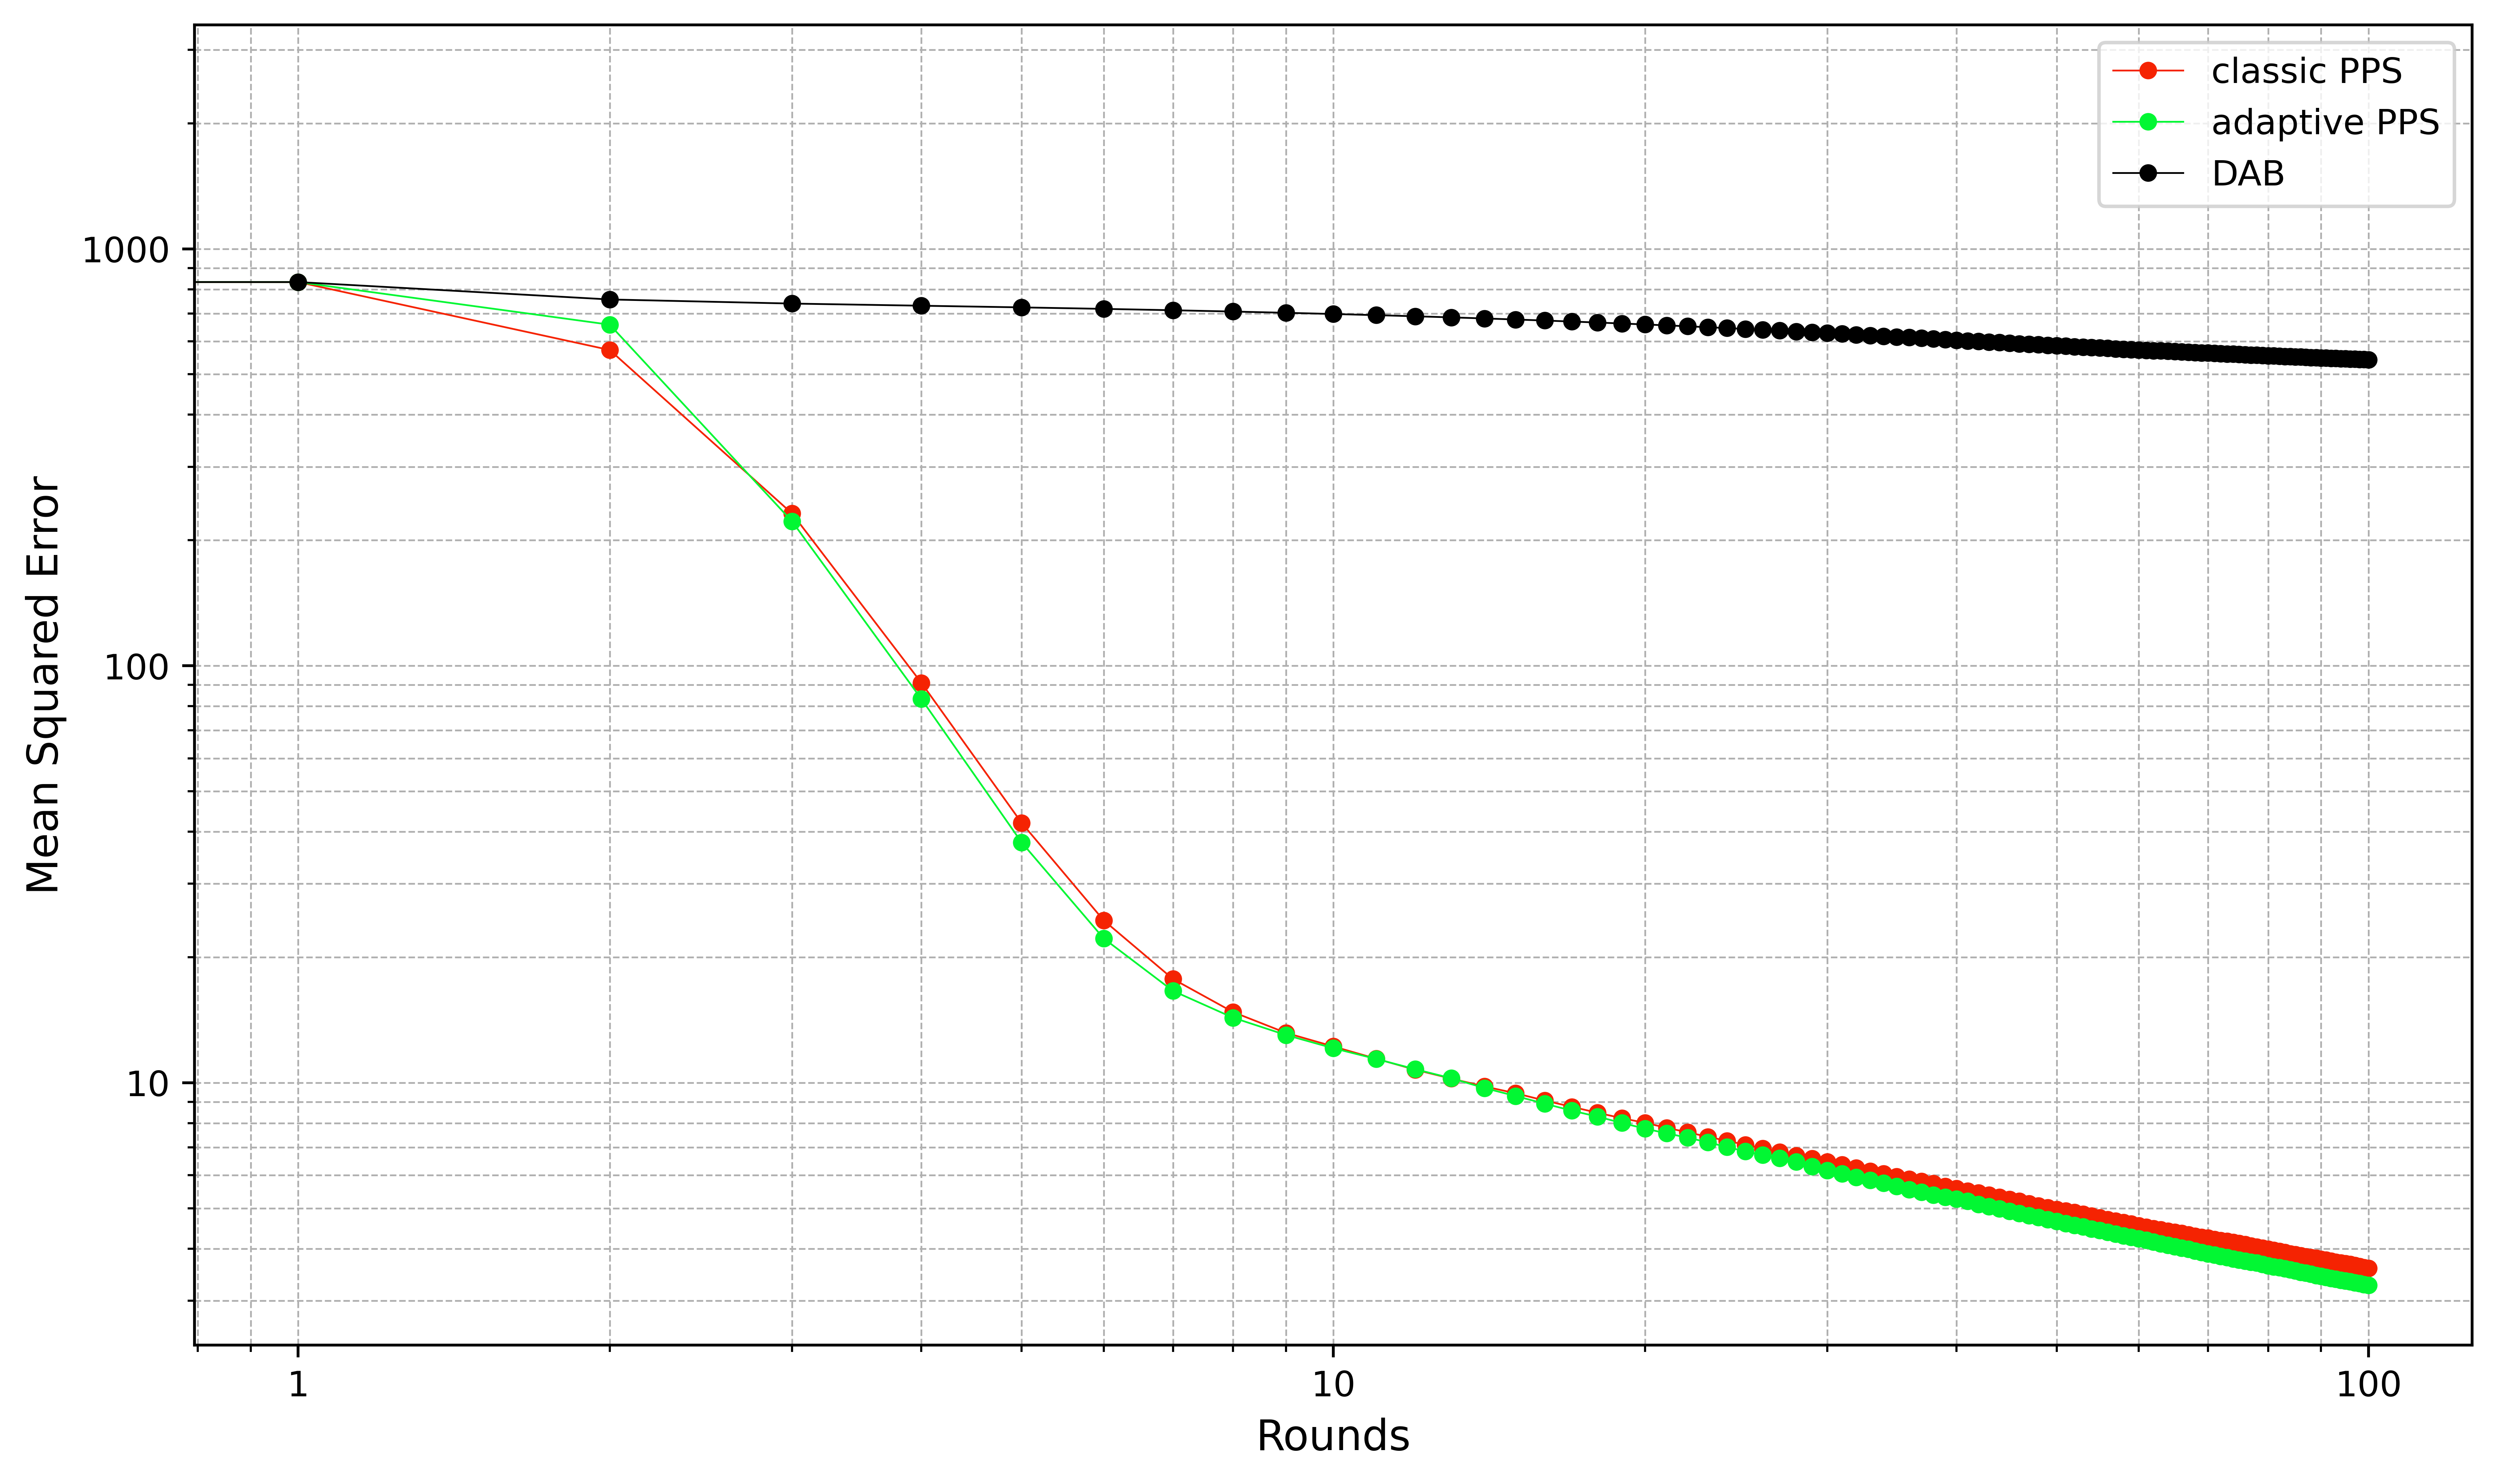
\includegraphics[width=0.49\linewidth]{figures/Simulation_outcomes/LollipopGraph/896_128/DAB_vs_PPS_LG_r100_n1024_averaged_loglog.png}}
    \caption{(896, 128)-Lollipop graph - mean squared error per rounds - log-linear
    and log-log}
        \label{fig:896_128lollipopgraphMSEperRoundLogLog}
\end{figure}

\begin{figure}[]
    \centering
    \scalebox{0.8}{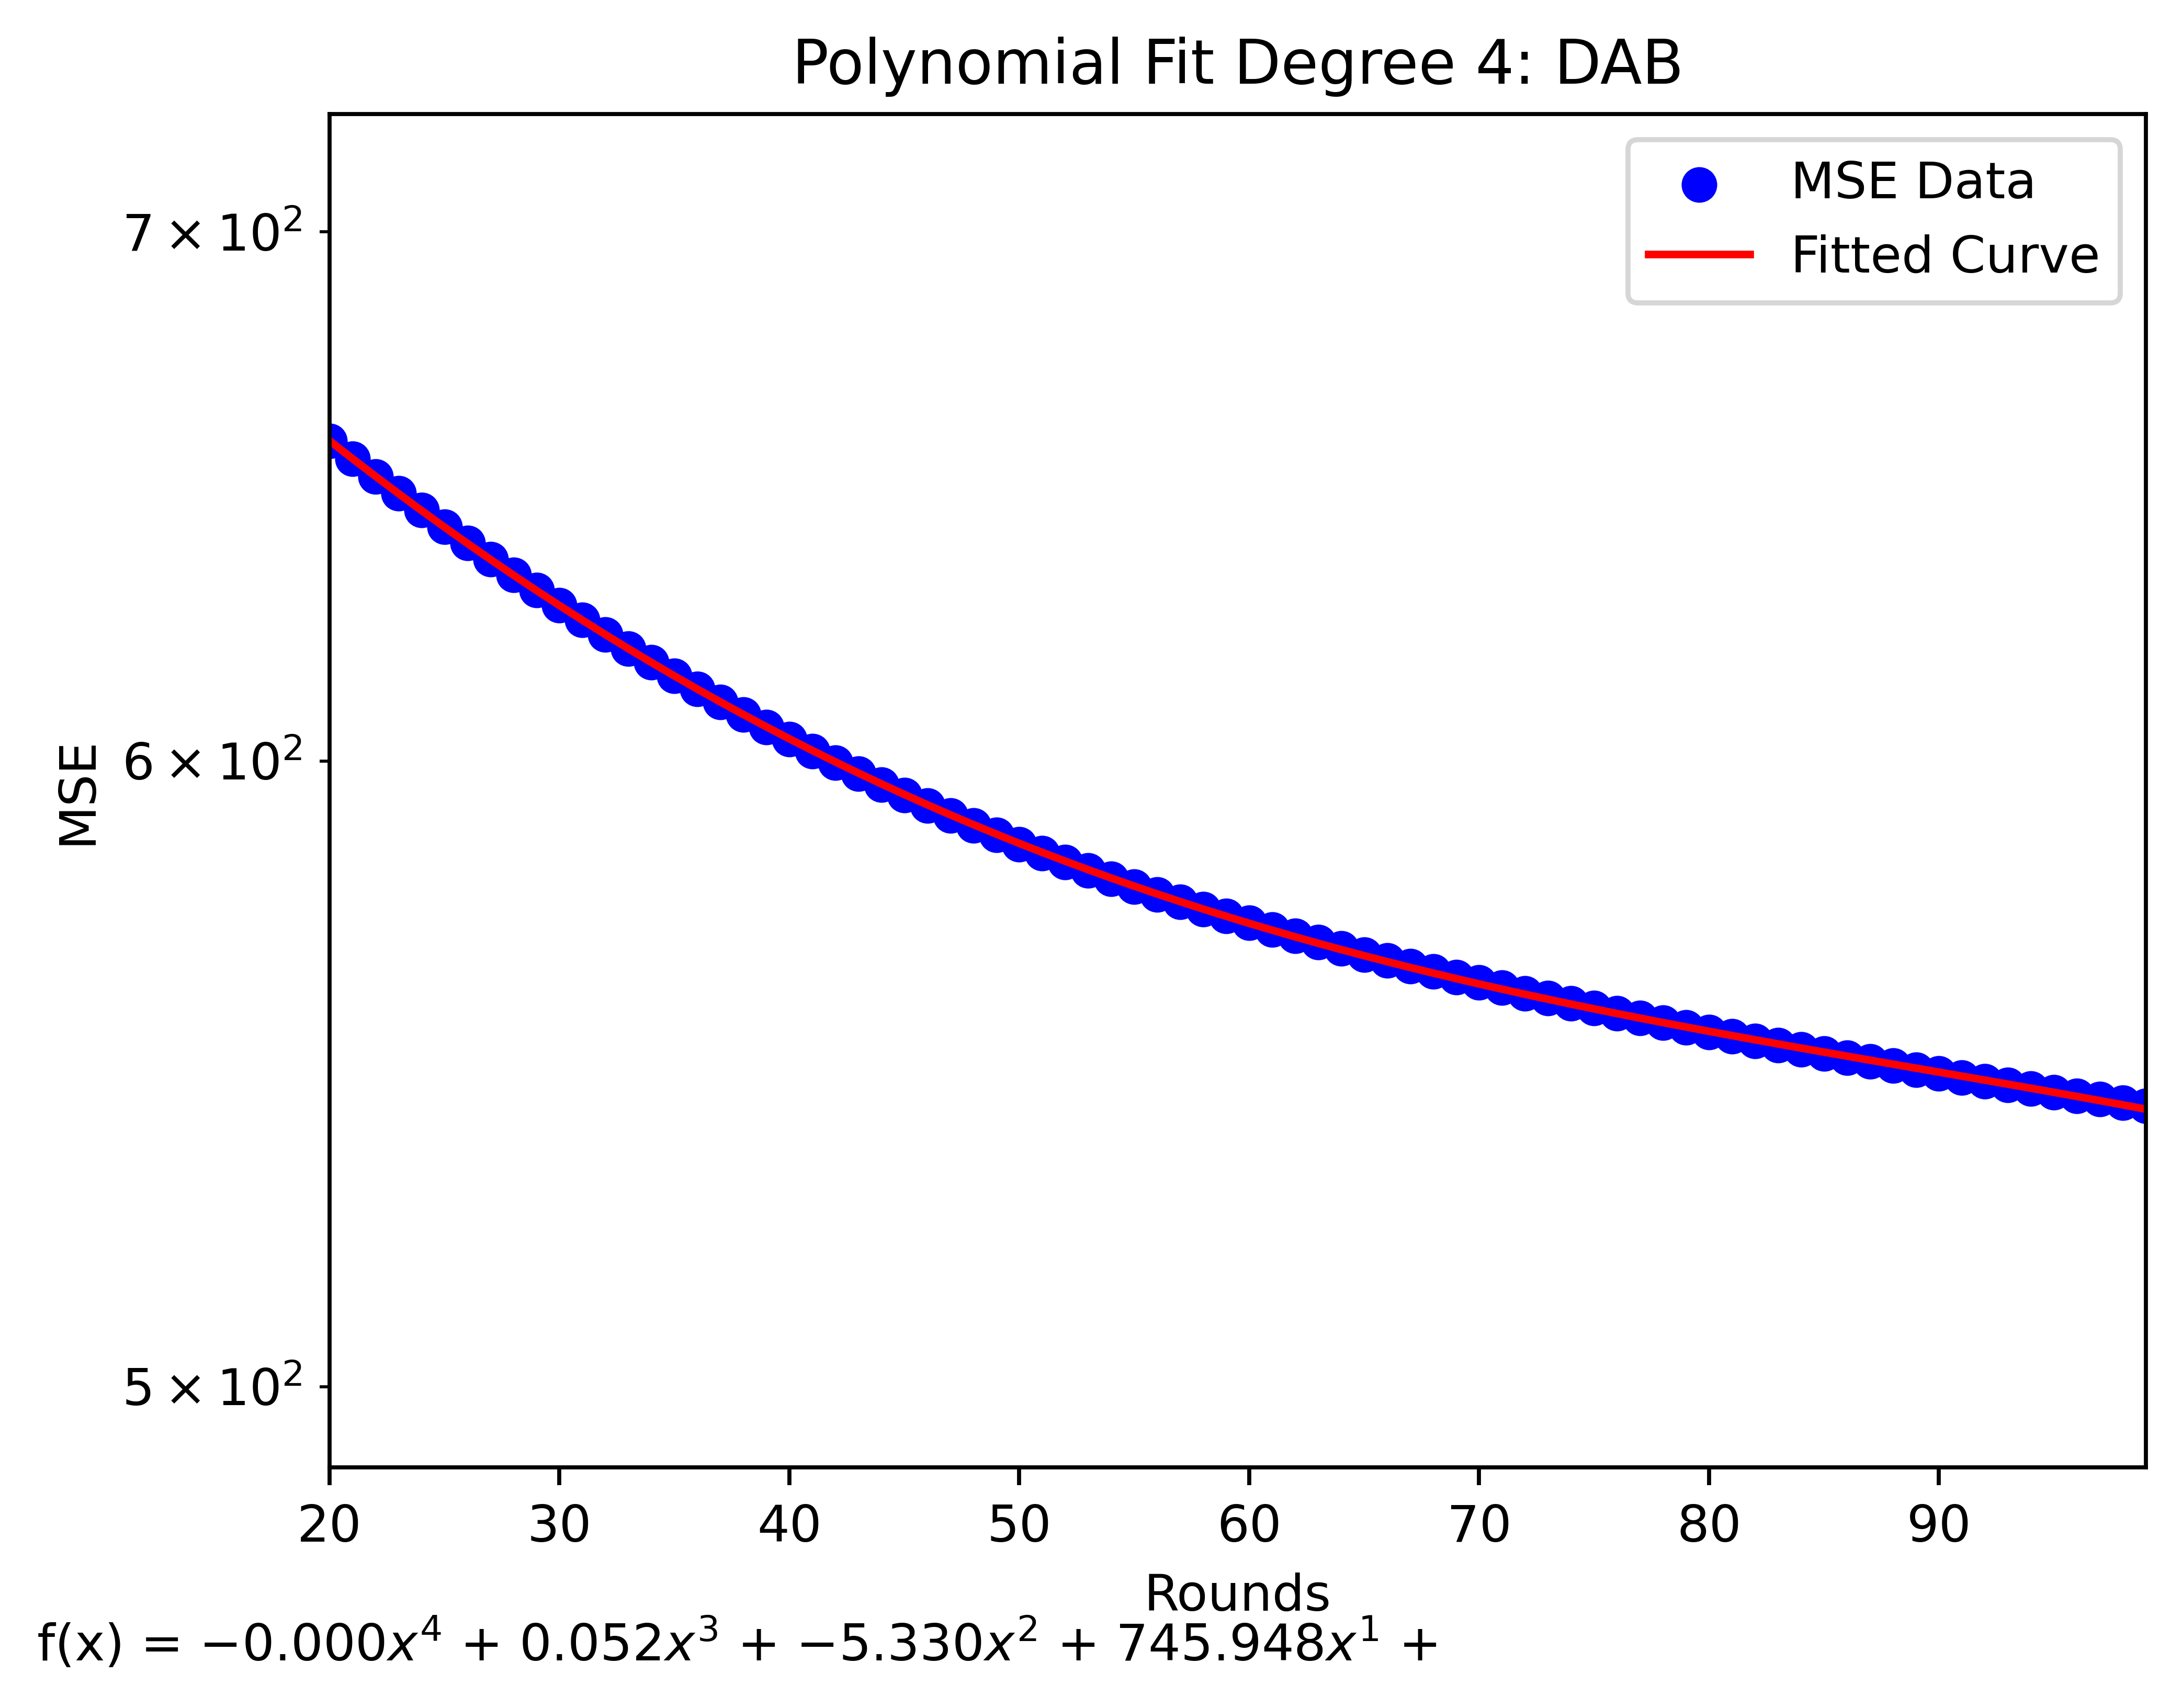
\includegraphics[width=\linewidth]{figures/Simulation_outcomes/LollipopGraph/896_128/DAB/DAB_modelfitting_rounds_99_model_2.png}}
    \caption{(896, 128)-Lollipop graph - polynomial regression fit - DAB}
    \label{fig:dab_896x128lollipopgraphModelFit}
\end{figure}

\begin{figure}[]
    \centering
    \scalebox{0.8}{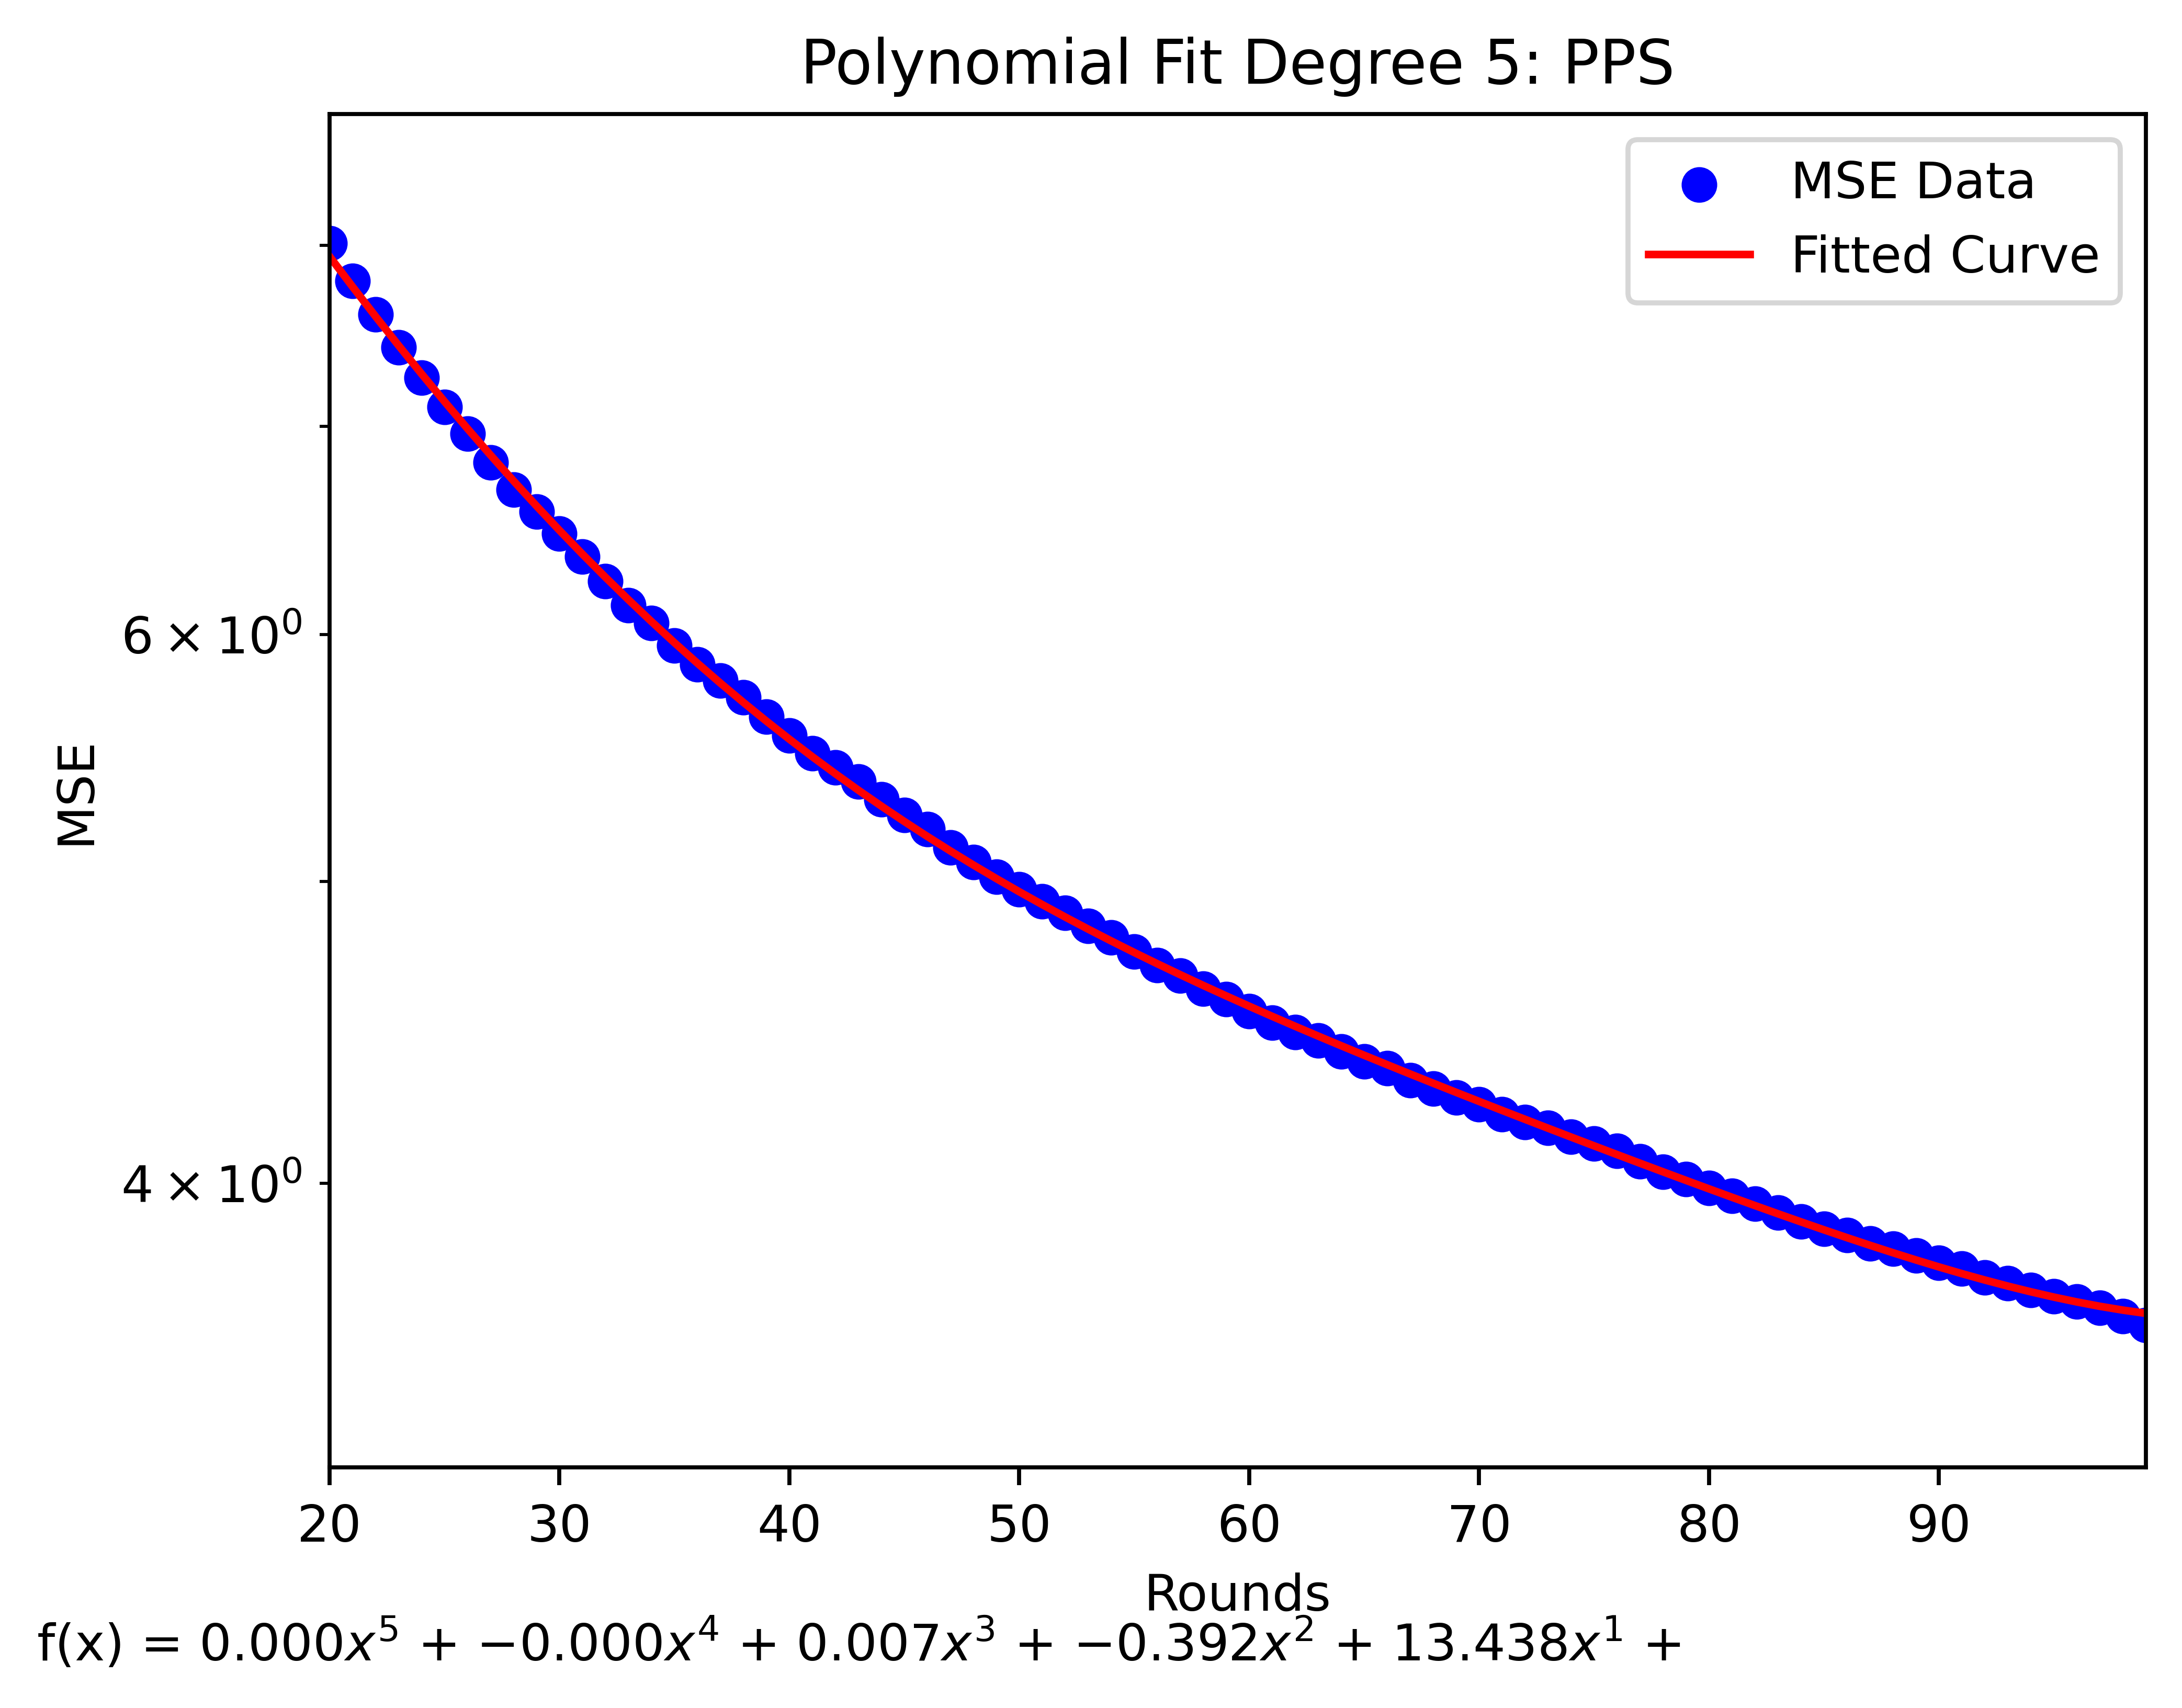
\includegraphics{figures/Simulation_outcomes/LollipopGraph/896_128/PPS/PPS_modelfitting_rounds_99_model_2.png}}
    \caption{(896, 128)-Lollipop graph - polynomial regression fit - PPS}
    \label{fig:pps_896x128lollipopgraphModelFit}
\end{figure}

\begin{figure}[]
    \centering
    \scalebox{0.8}{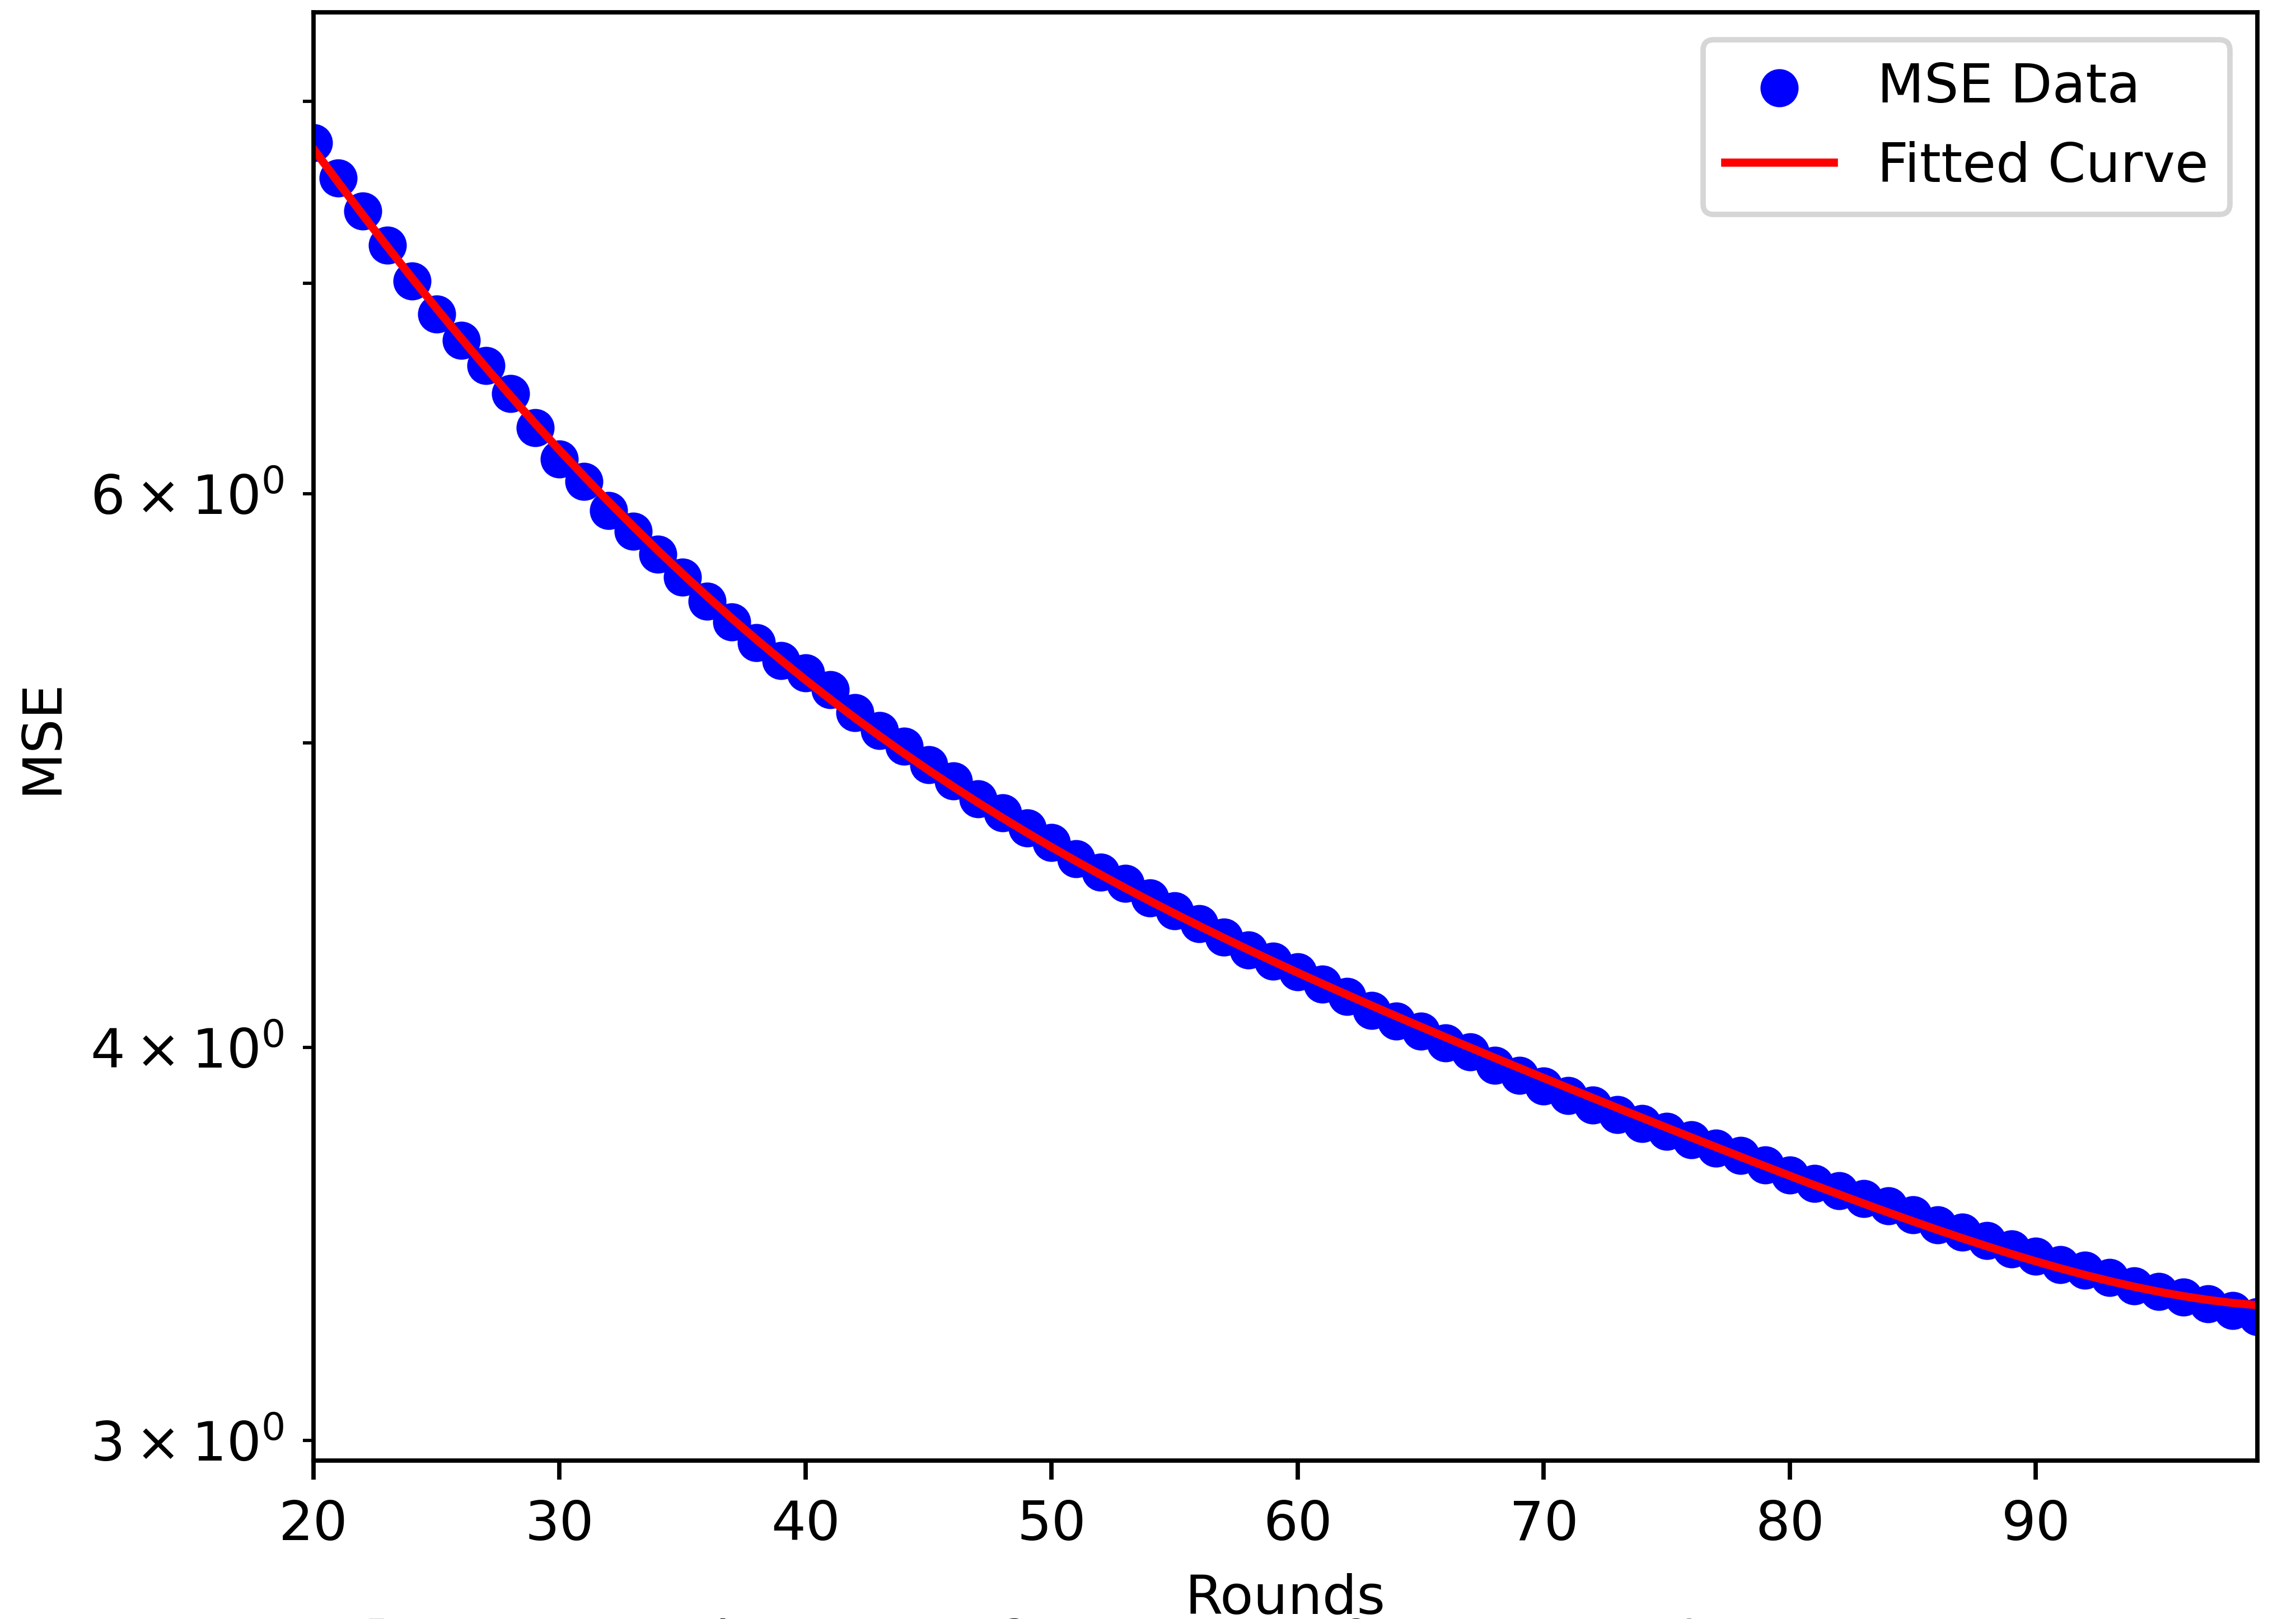
\includegraphics[width=\linewidth]{figures/Simulation_outcomes/LollipopGraph/896_128/ATPPS/ATPPS_modelfitting_rounds_99_model_2.png}}
    \caption{(896, 128)-Lollipop graph - polynomial regression fit - ATPPS}
    \label{fig:atpps_896x128lollipopgraphModelFit}
\end{figure}

\begin{figure}[!ht]
    \centering
        \subfloat[]{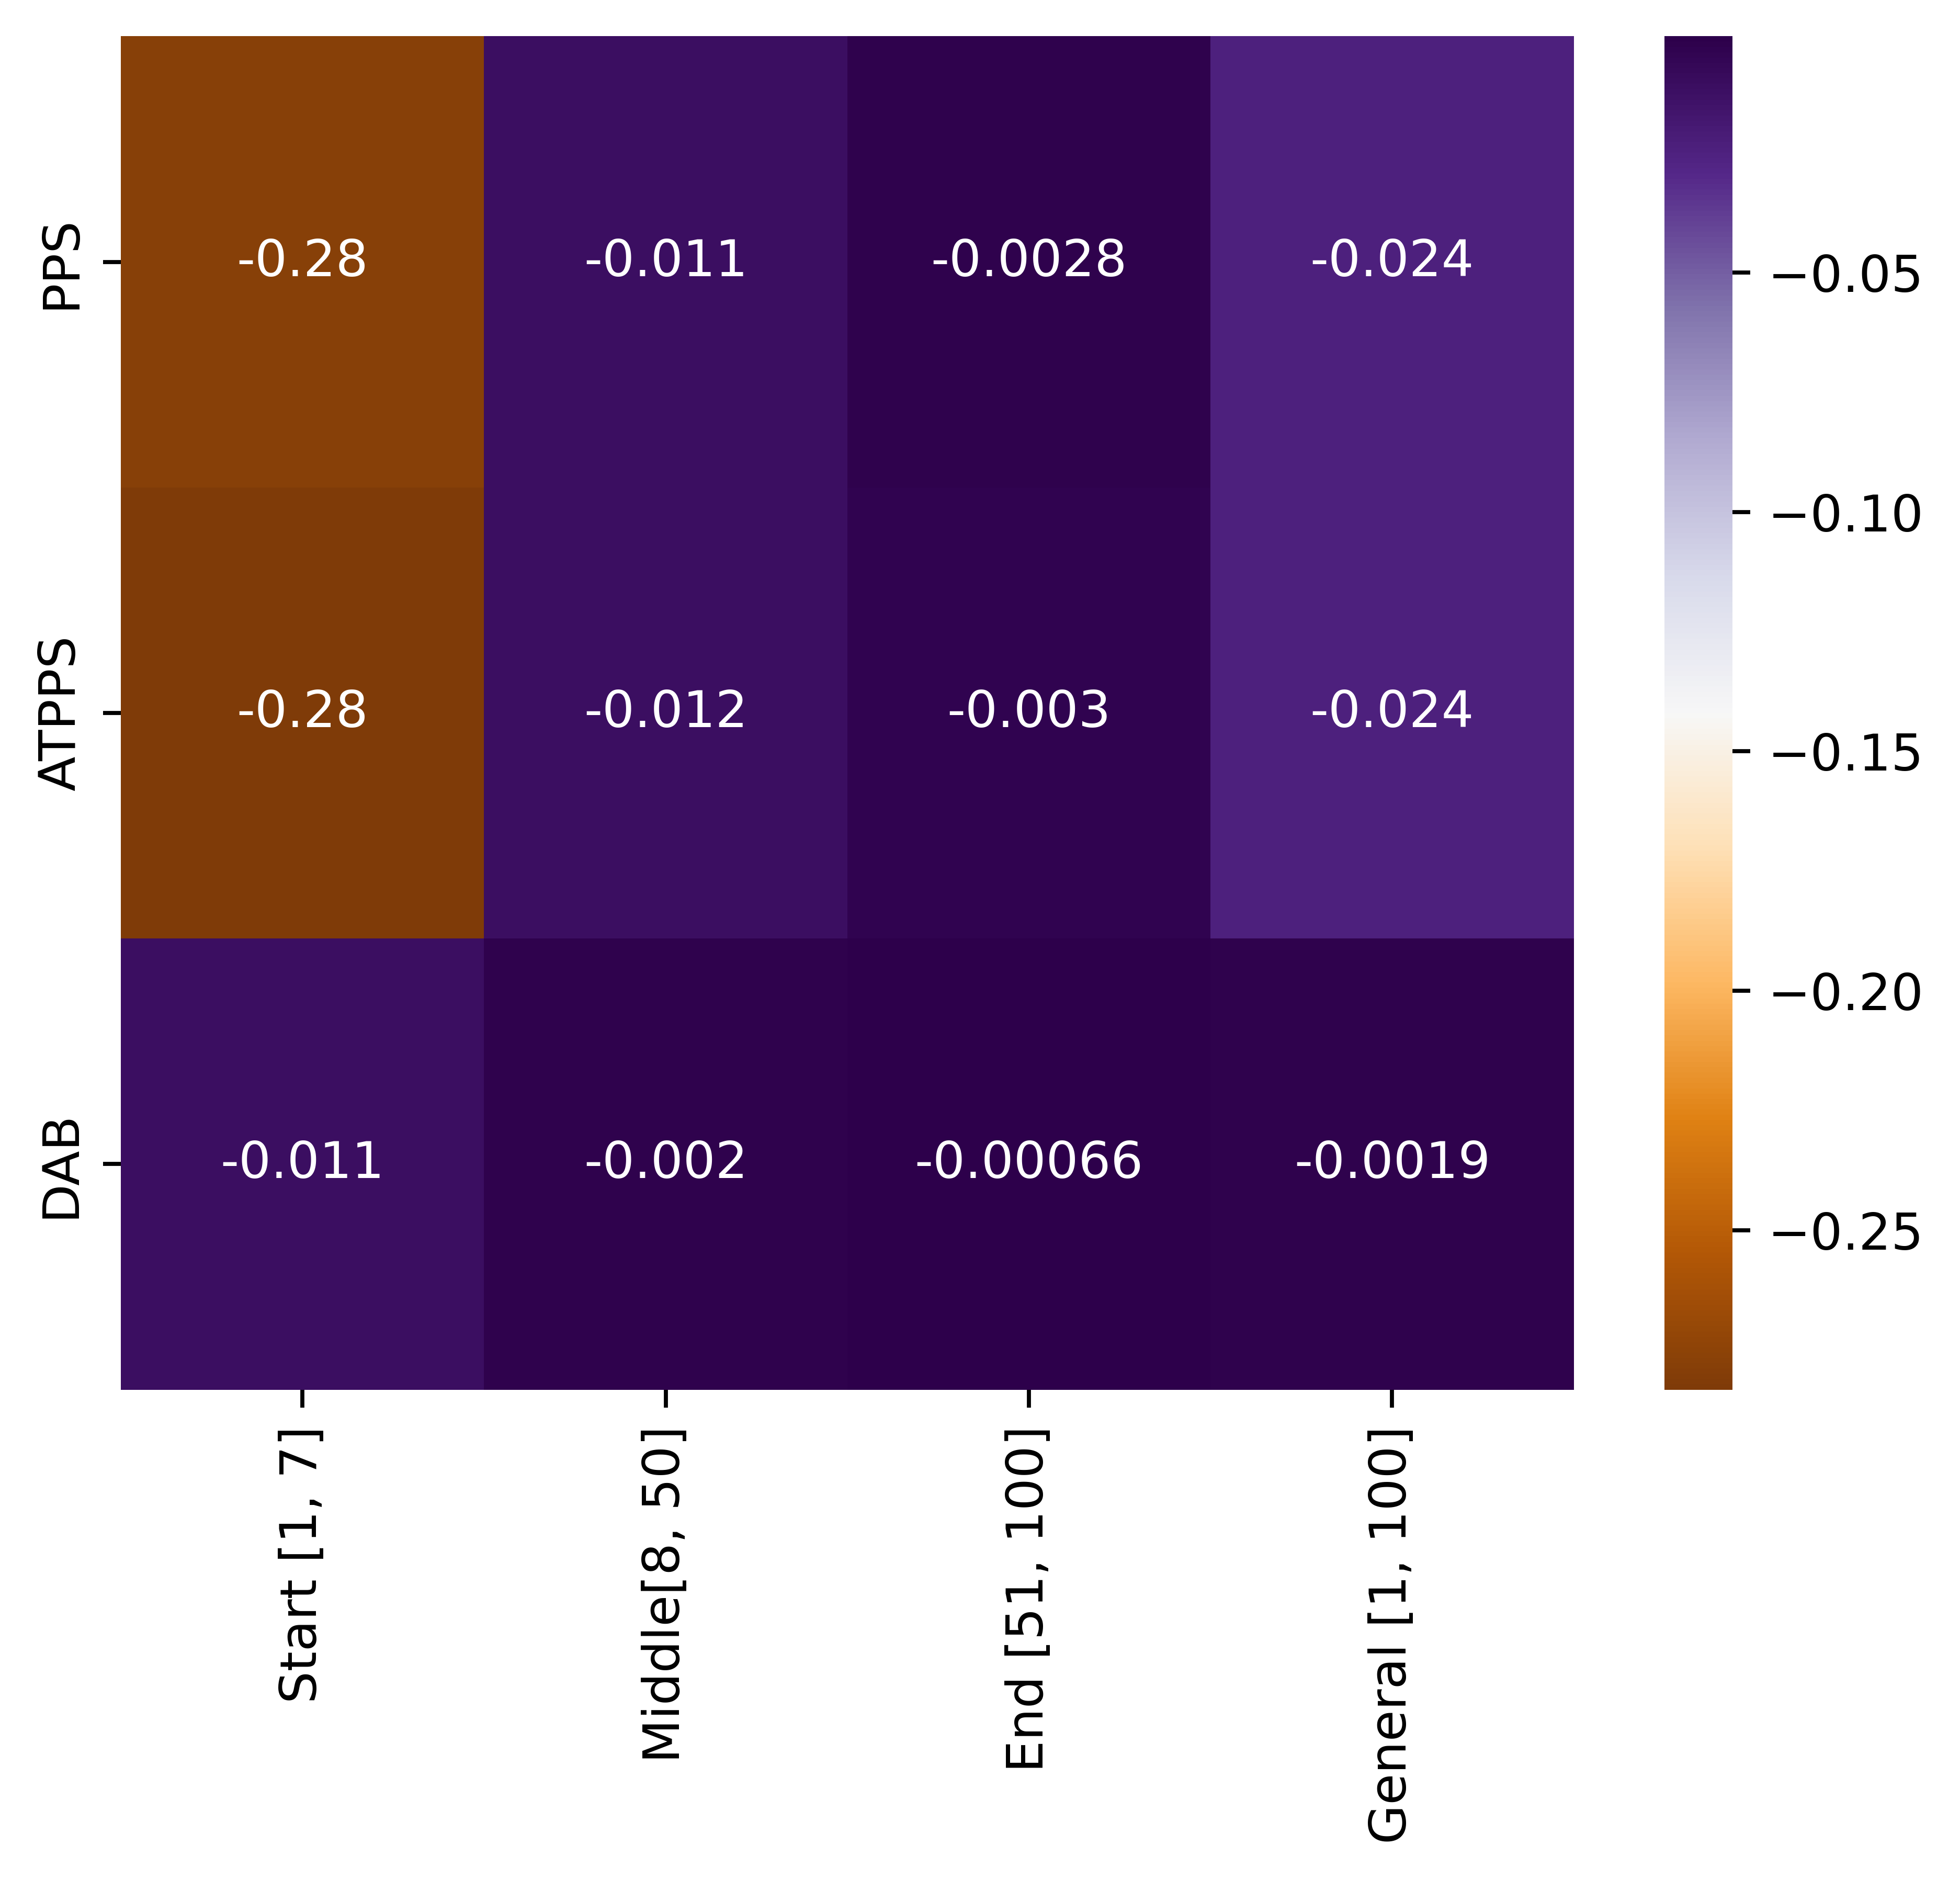
\includegraphics[width=0.49\linewidth]{figures/Simulation_outcomes/LollipopGraph/896_128/DAB_vs_PPS_vs_ATPPS_slopesheatmap_100rounds_log_linear.png}}
    \hfil
        \subfloat[]{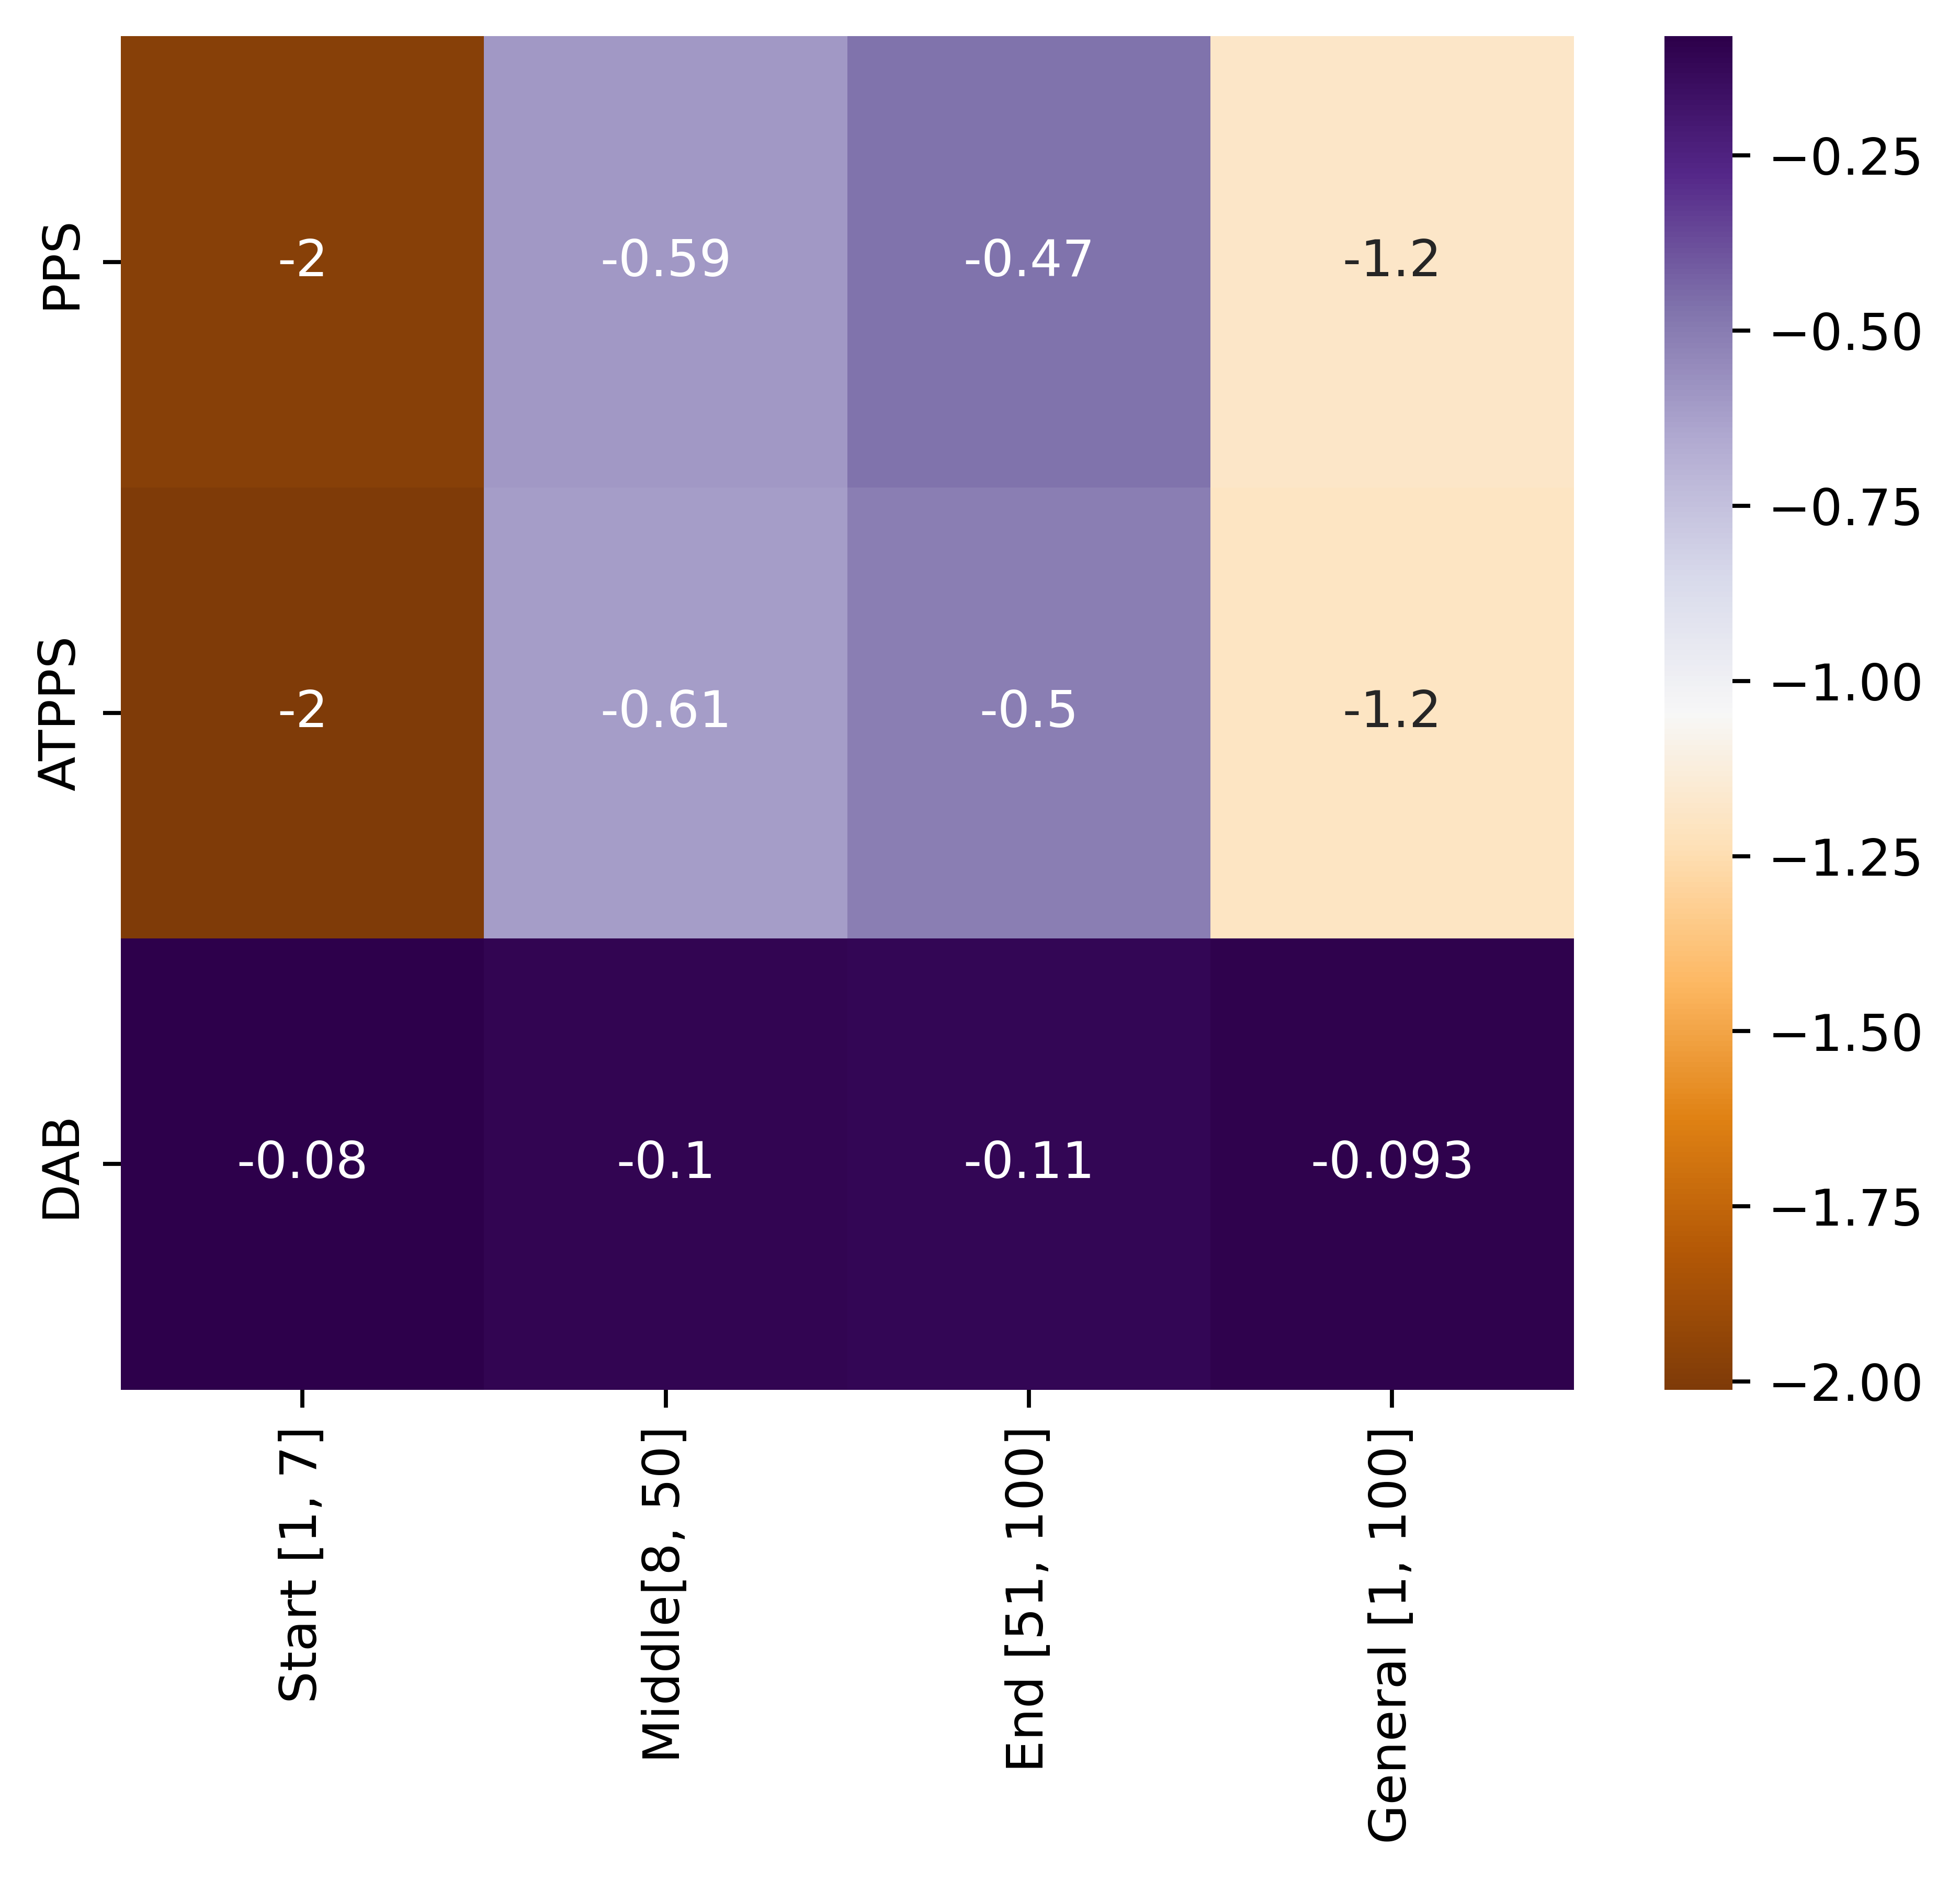
\includegraphics[width=0.49\linewidth]{figures/Simulation_outcomes/LollipopGraph/896_128/DAB_vs_PPS_vs_ATPPS_slopesheatmap_100rounds_log_log.png}}
    \caption{(896, 128)-Lollipop graph - heat map of slopes per region - log-linear and log-log}
        \label{fig:896x128lollipopslopes}
\end{figure}

\section{Ring of Cliques}\label{sec:ringofcliques}
\subsection{(32 x 32)-Ring of Cliques}\label{subsec:32_32ROC}
In the early rounds, PPS and ATPPS exhibit the fastest MSE reduction, as shown by a very steep downward trend between rounds 1 and 5 in figure \ref{fig:atppsRingOfCliquesLog_LogLog} b). Both Push-Pull Sum-based approaches demonstrate faster convergence rates compared to DAB in the $(32\times 32)$-Ring of Cliques $ROC_{32,32}$. The initial steep downward slope of around -1.8 for each Push-Pull Sum-based algorithm, as depicted in figure \ref{fig:ringOfCliquesslopes}, within the first 5 rounds is due to the fact that each clique is balanced efficiently by these algorithms. The Push-Pull Sum-based algorithms perform better than DAB in high-degree cliques. Once the cliques start to balance, round by round, DAB catches up, especially between rounds 6 and 40, where the slopes are -2.1 for the DAB compared to approximately $-0.5$ for the Push-Pull Sum-based algorithms. Nodes within cliques tend to converge quickly internally due to their dense interconnections for the Push-Pull Sum-based algorithms. However, load balancing between cliques, especially when the nodes select random neighbors, is slower, creating bottlenecks for global convergence (this is especially the case for the PPS, whose curve starts to stagnate between round 10 and 100). Thanks to the deterministic load balancing strategies, the bridging nodes start to spread the load to other cliques. The ATPPS achieves better results compared to the PPS since it has a similar mechanism in this scenario like the DAB, prioritizing communication between cliques (where differences in loads are more significant) over redundant communication within cliques (where loads are already close to balanced). This is reflected in the behavior of the curve after round 10. Again, the ATPPS acts as a compromise solution between the PPS and the DAB, achieving results close to those of the DAB. Overall, at round 100 the DAB achieved an MSE of approximately $6.55$, the PPS an MSE of 19.80, and the ATPPS an MSE of 8.42.

The polynomial fit for the DAB is expressed as:
\begin{align}
    MSE_r=1.04\times 10^{-6}r^{4}-2.94\times 10^{-4}r^{3}+0.03r^{2}-1.66r+45.30    
\end{align}
(figure \ref{fig:dabRingOfCliquesModelFit}), which models the MSE data as a function of rounds with a fourth-degree polynomial. For the PPS, the MSE data from rounds 20 to 100 is fitted to a linear regression model:
\begin{align}
    MSE_r=-0.05r+24.70
\end{align}
(figure \ref{fig:ppsRingOfCliquesModelFit}). The negative slope indicates a consistent reduction in MSE with each round in this region, though the value -0.05 is relatively small. This suggests that the PPS achieves slow and steady progress toward a balanced network. The linear fit indicates that PPS achieves only gradual improvement in balancing the load in $ROC_{32,32}$. The reason for that is that PPS focuses on a push-pull mechanism that is, relying on random neighbor interactions. In the Ring of Cliques, inter-clique connections are sparse, and PPS lacks a mechanism to prioritize balancing between these sparsely connected regions. As a result, its performance is bottlenecked by the topology. The linear regression model highlights a uniform rate of error reduction over the rounds, with no acceleration observed, unlike other approaches like DAB. The logarithmic model for the ATPPS is given by: 
\begin{align}
    \log{(MSE_r)}=-7.59\log{(r)}+43.26   
\end{align}
(figure \ref{fig:atppsRingOfCliquesModelFit}). By exponentiating this equation, the relationship between MSE and the number of rounds can be written as:
\begin{align}
    MSE_r=r^{-7.59}*10^{43.26}.    
\end{align}
The steep negative slope of -7.59 in the log-log fit indicates a rapid decrease in MSE as the number of rounds increases. This suggests that ATPPS achieves exponentially faster convergence compared to PPS, particularly in the early rounds of load balancing.

\begin{figure}[!ht]
    \centering
        \subfloat[]{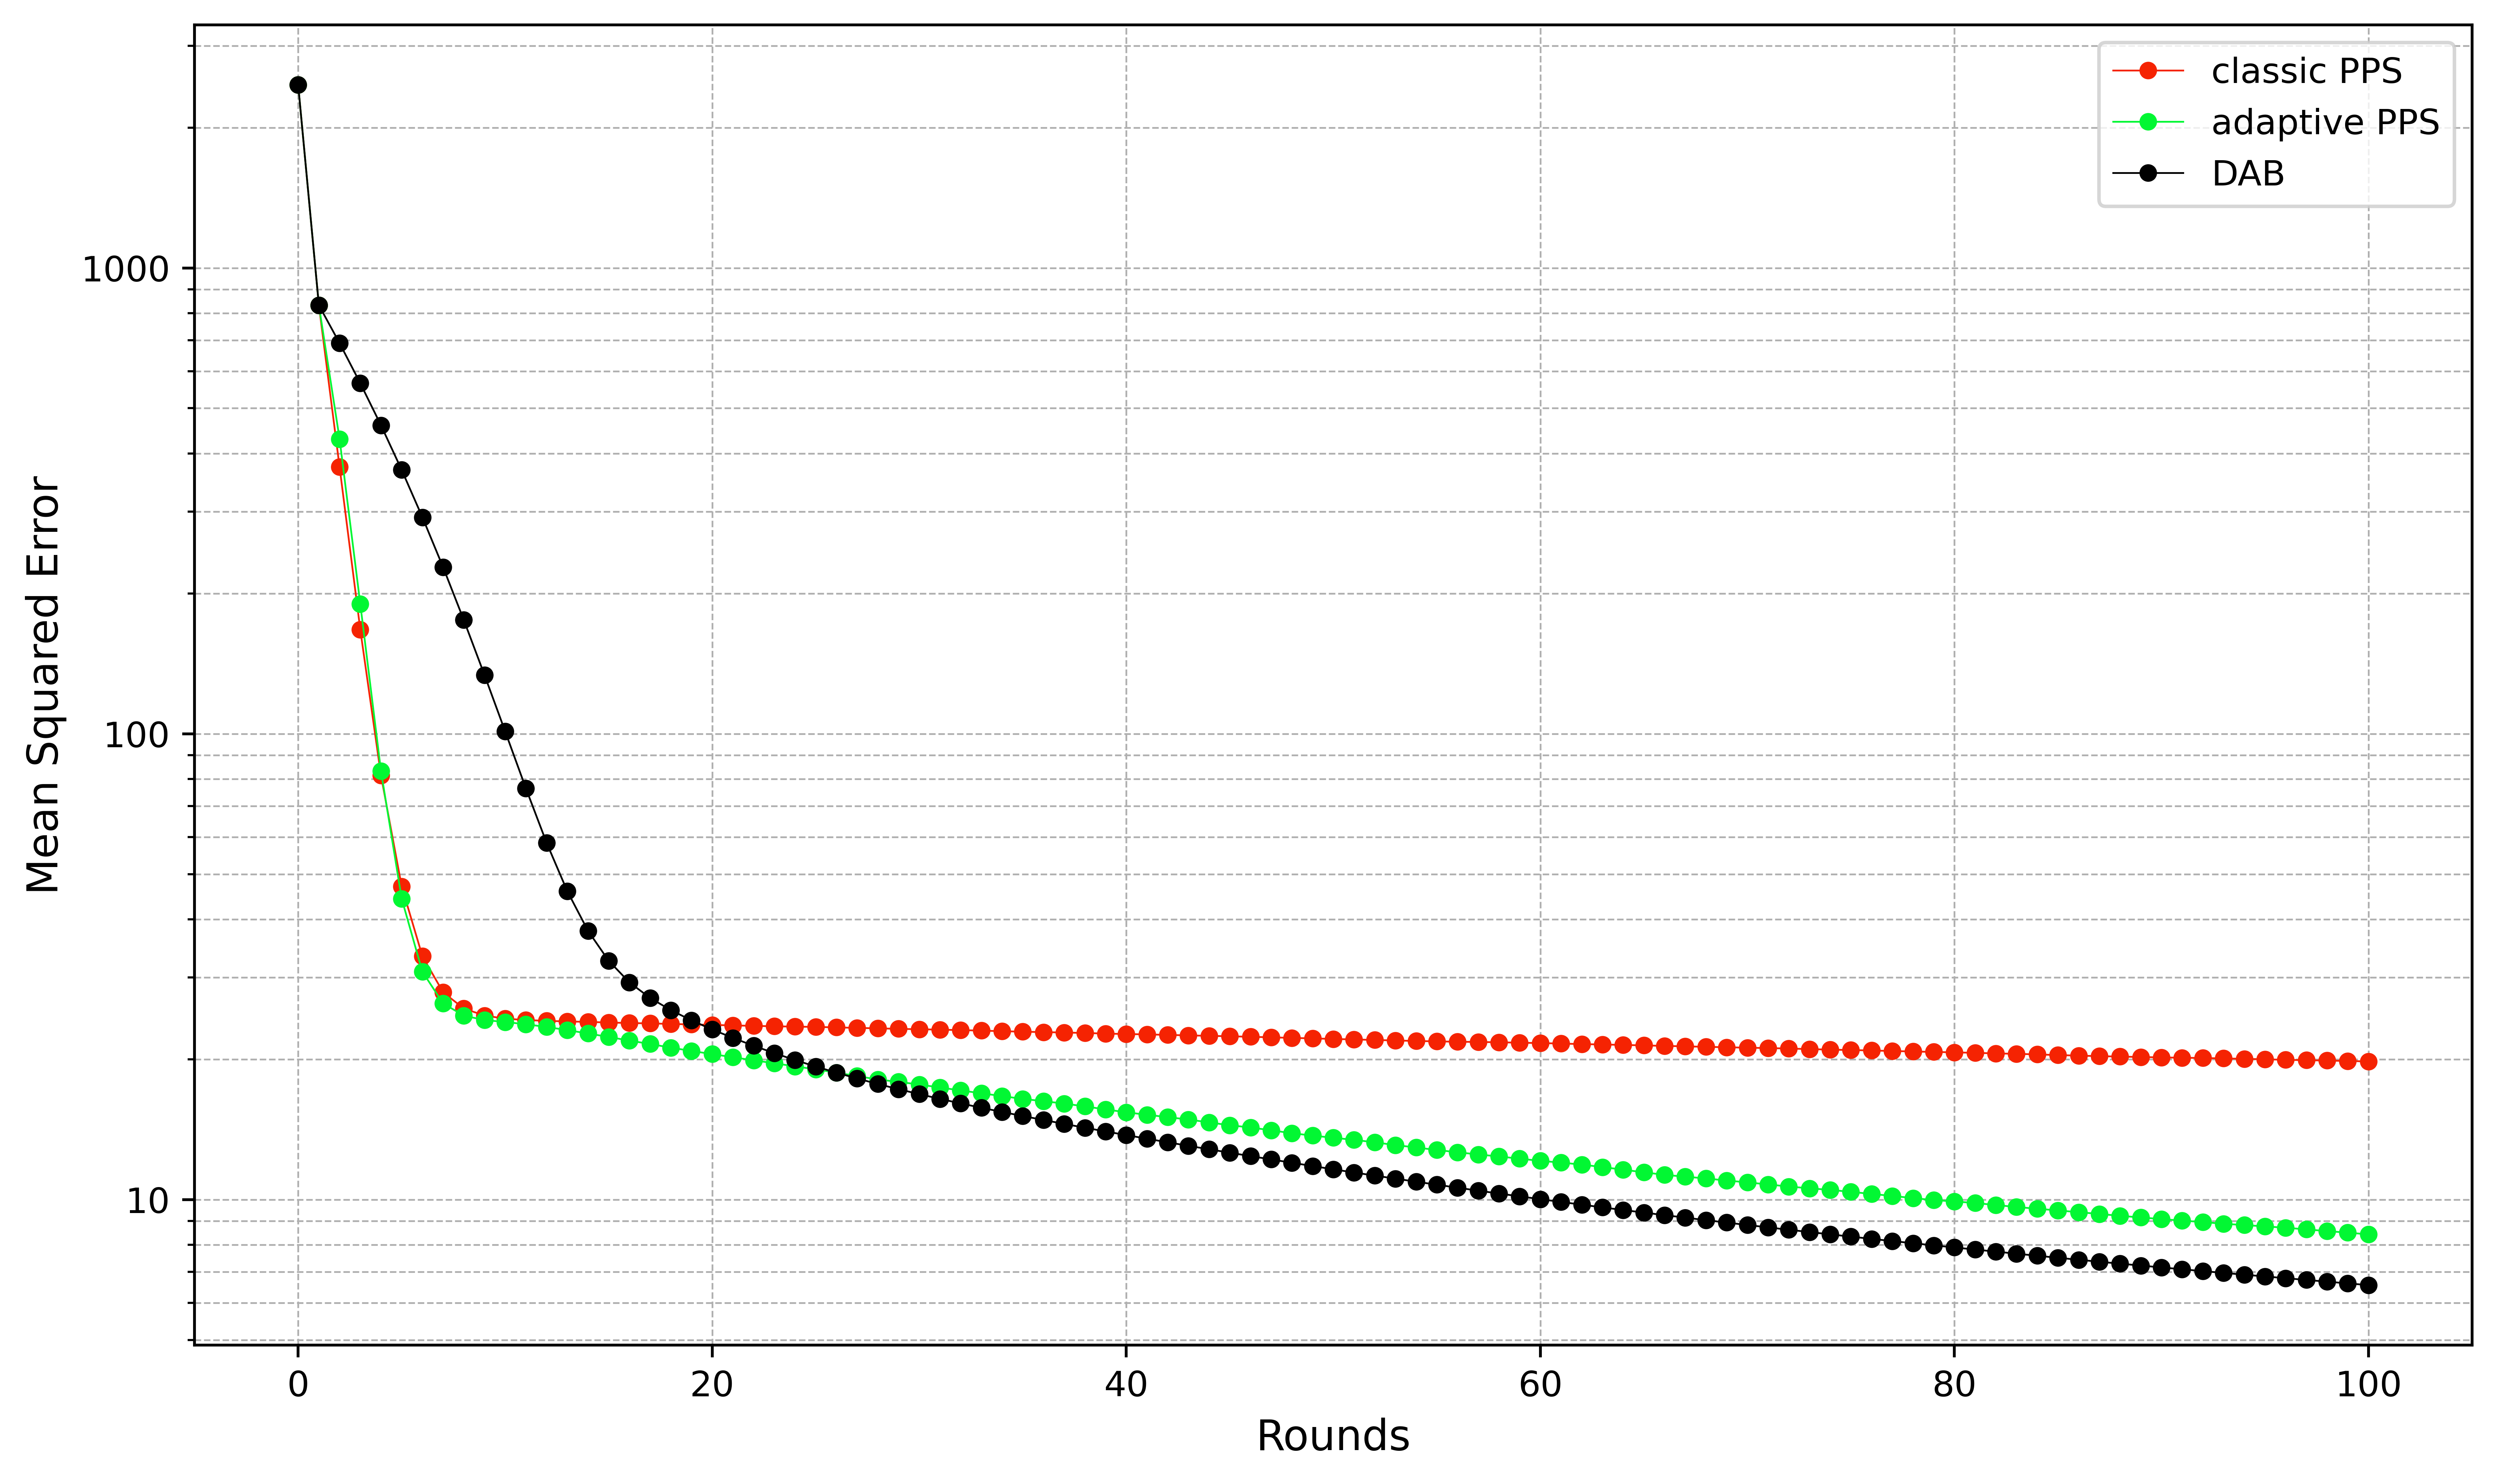
\includegraphics[width=0.49\linewidth]{figures/Simulation_outcomes/RingOfCliques/32x32/DAB_vs_PPS_RoC_r100_n1024_averaged_log.png}}
    \hfil
        \subfloat[]{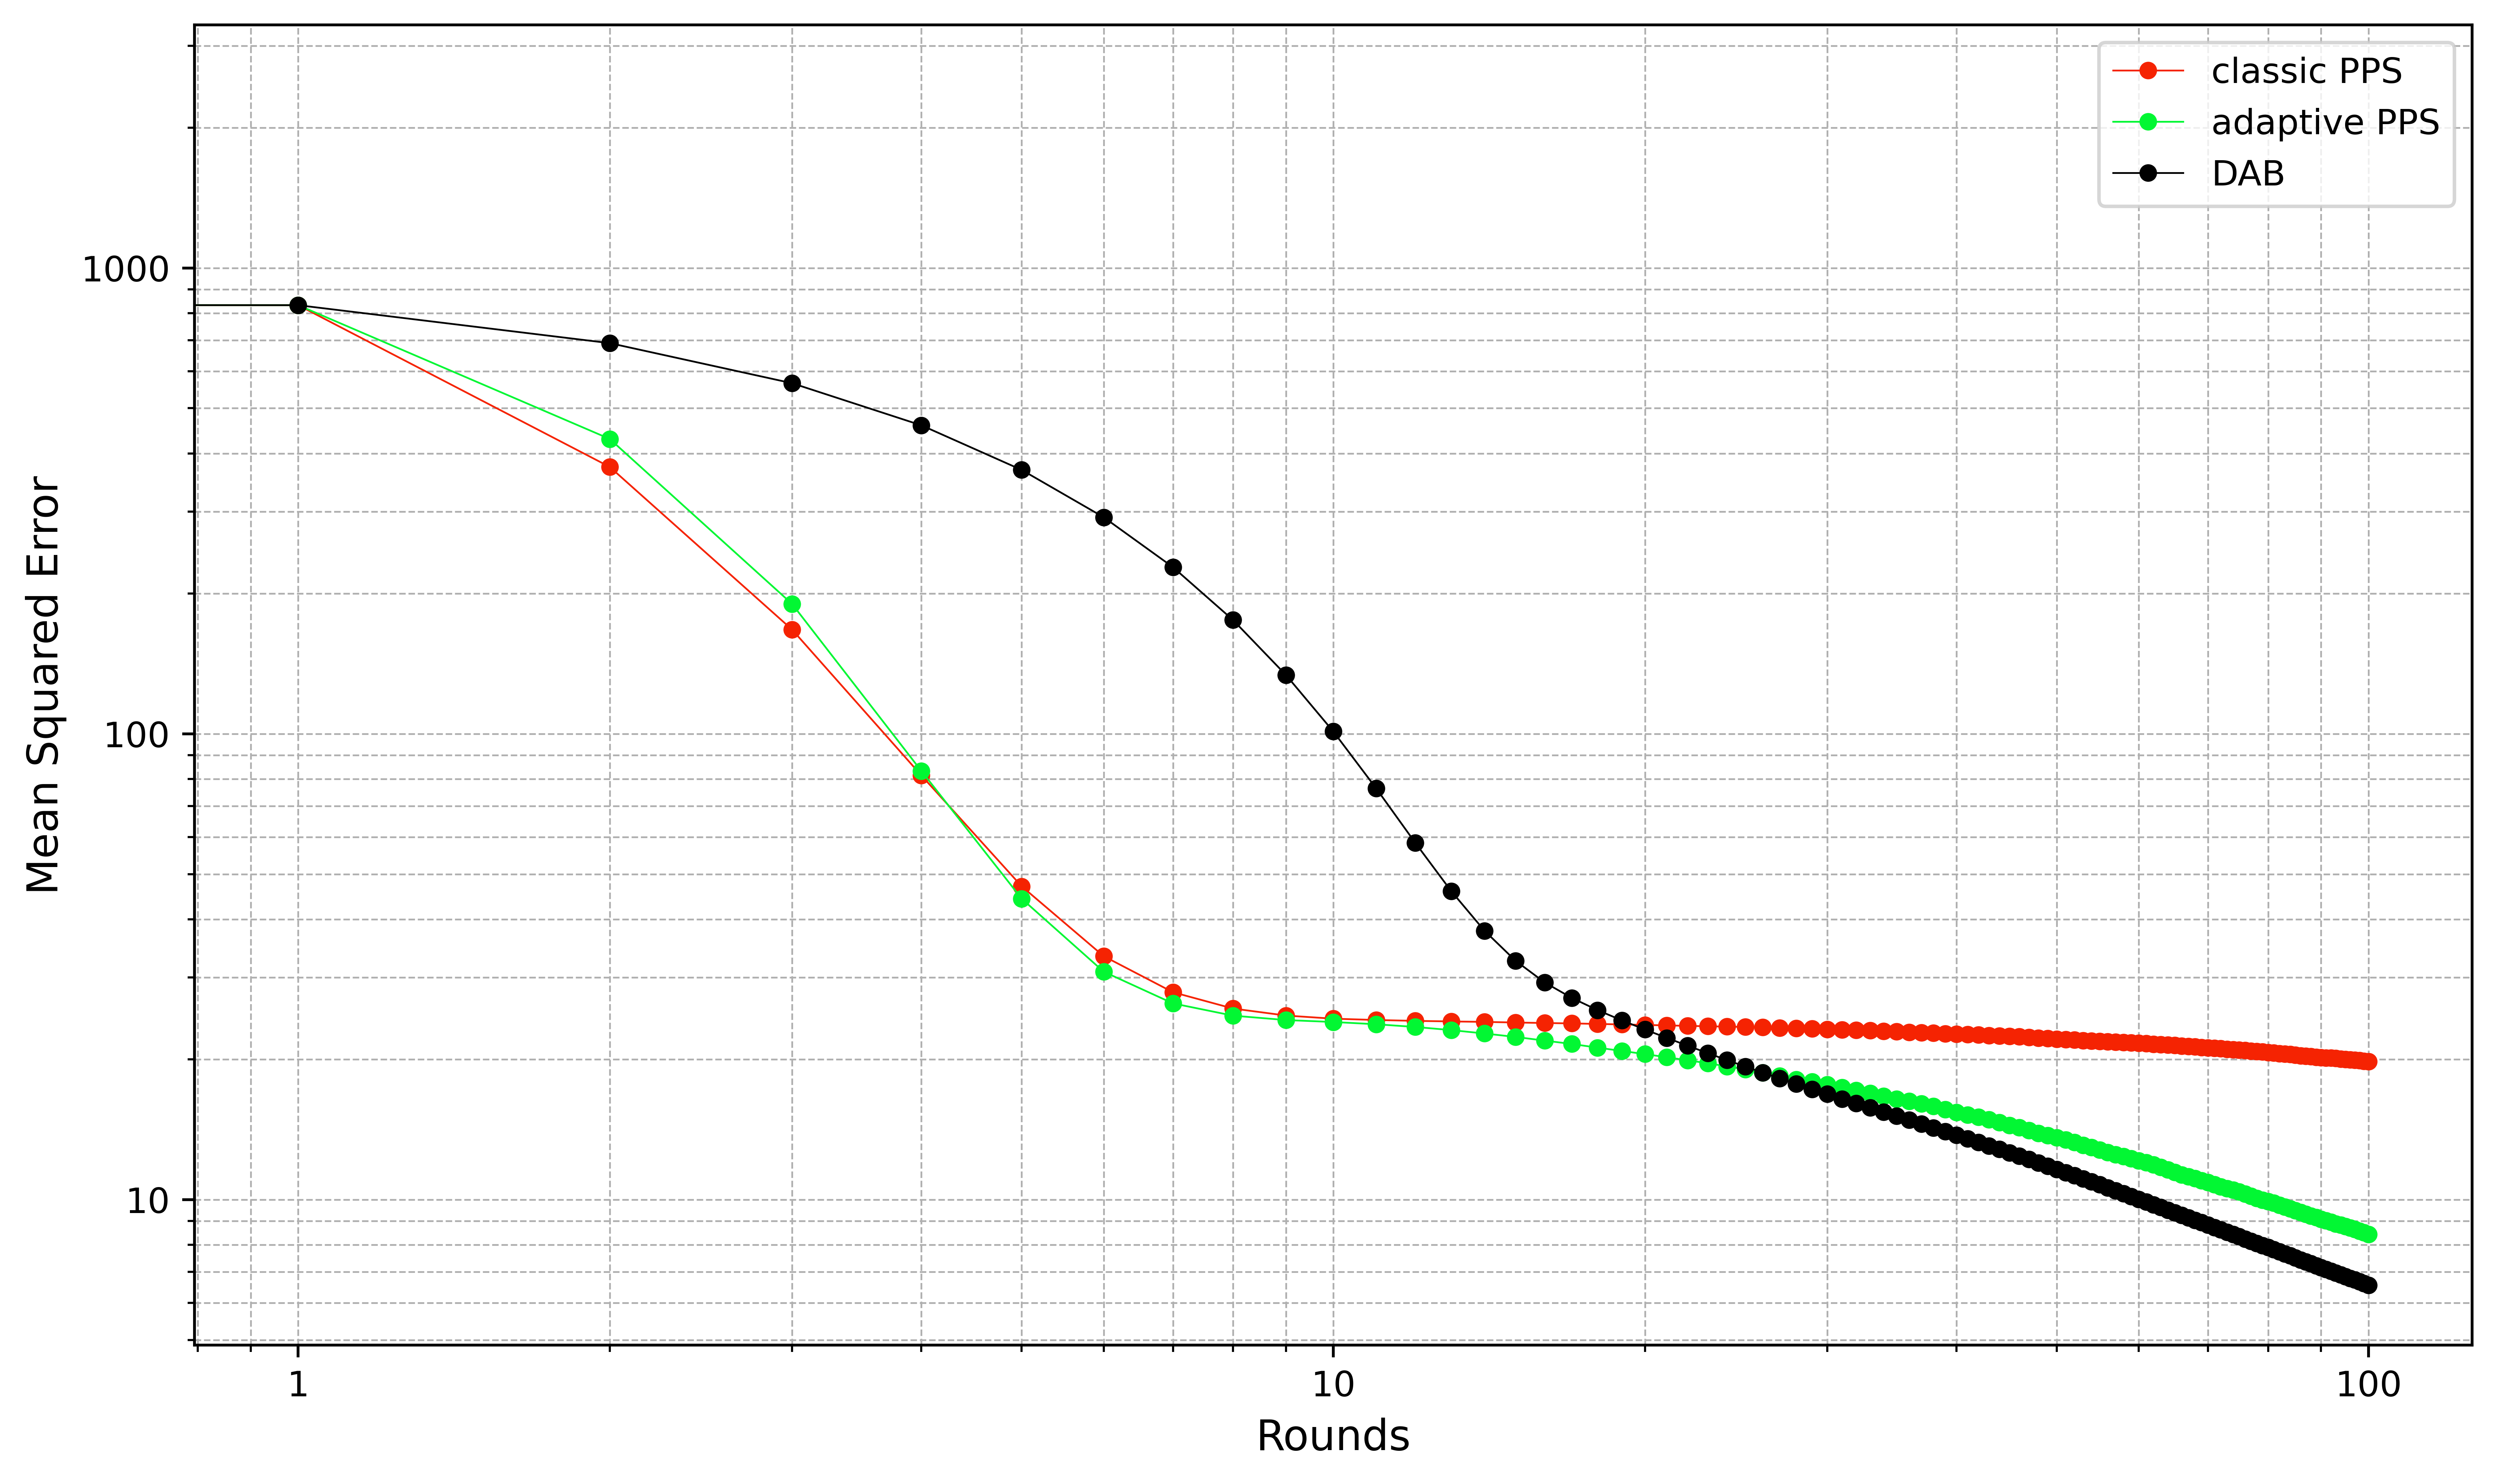
\includegraphics[width=0.49\linewidth]{figures/Simulation_outcomes/RingOfCliques/32x32/DAB_vs_PPS_RoC_r100_n1024_averaged_loglog.png}}
    \caption{$(32\times32)$-Ring of Cliques - mean squared error per rounds - log-linear and log-log}
        \label{fig:atppsRingOfCliquesLog_LogLog}
\end{figure}
 \begin{figure}[]
     \centering
     \scalebox{0.8}{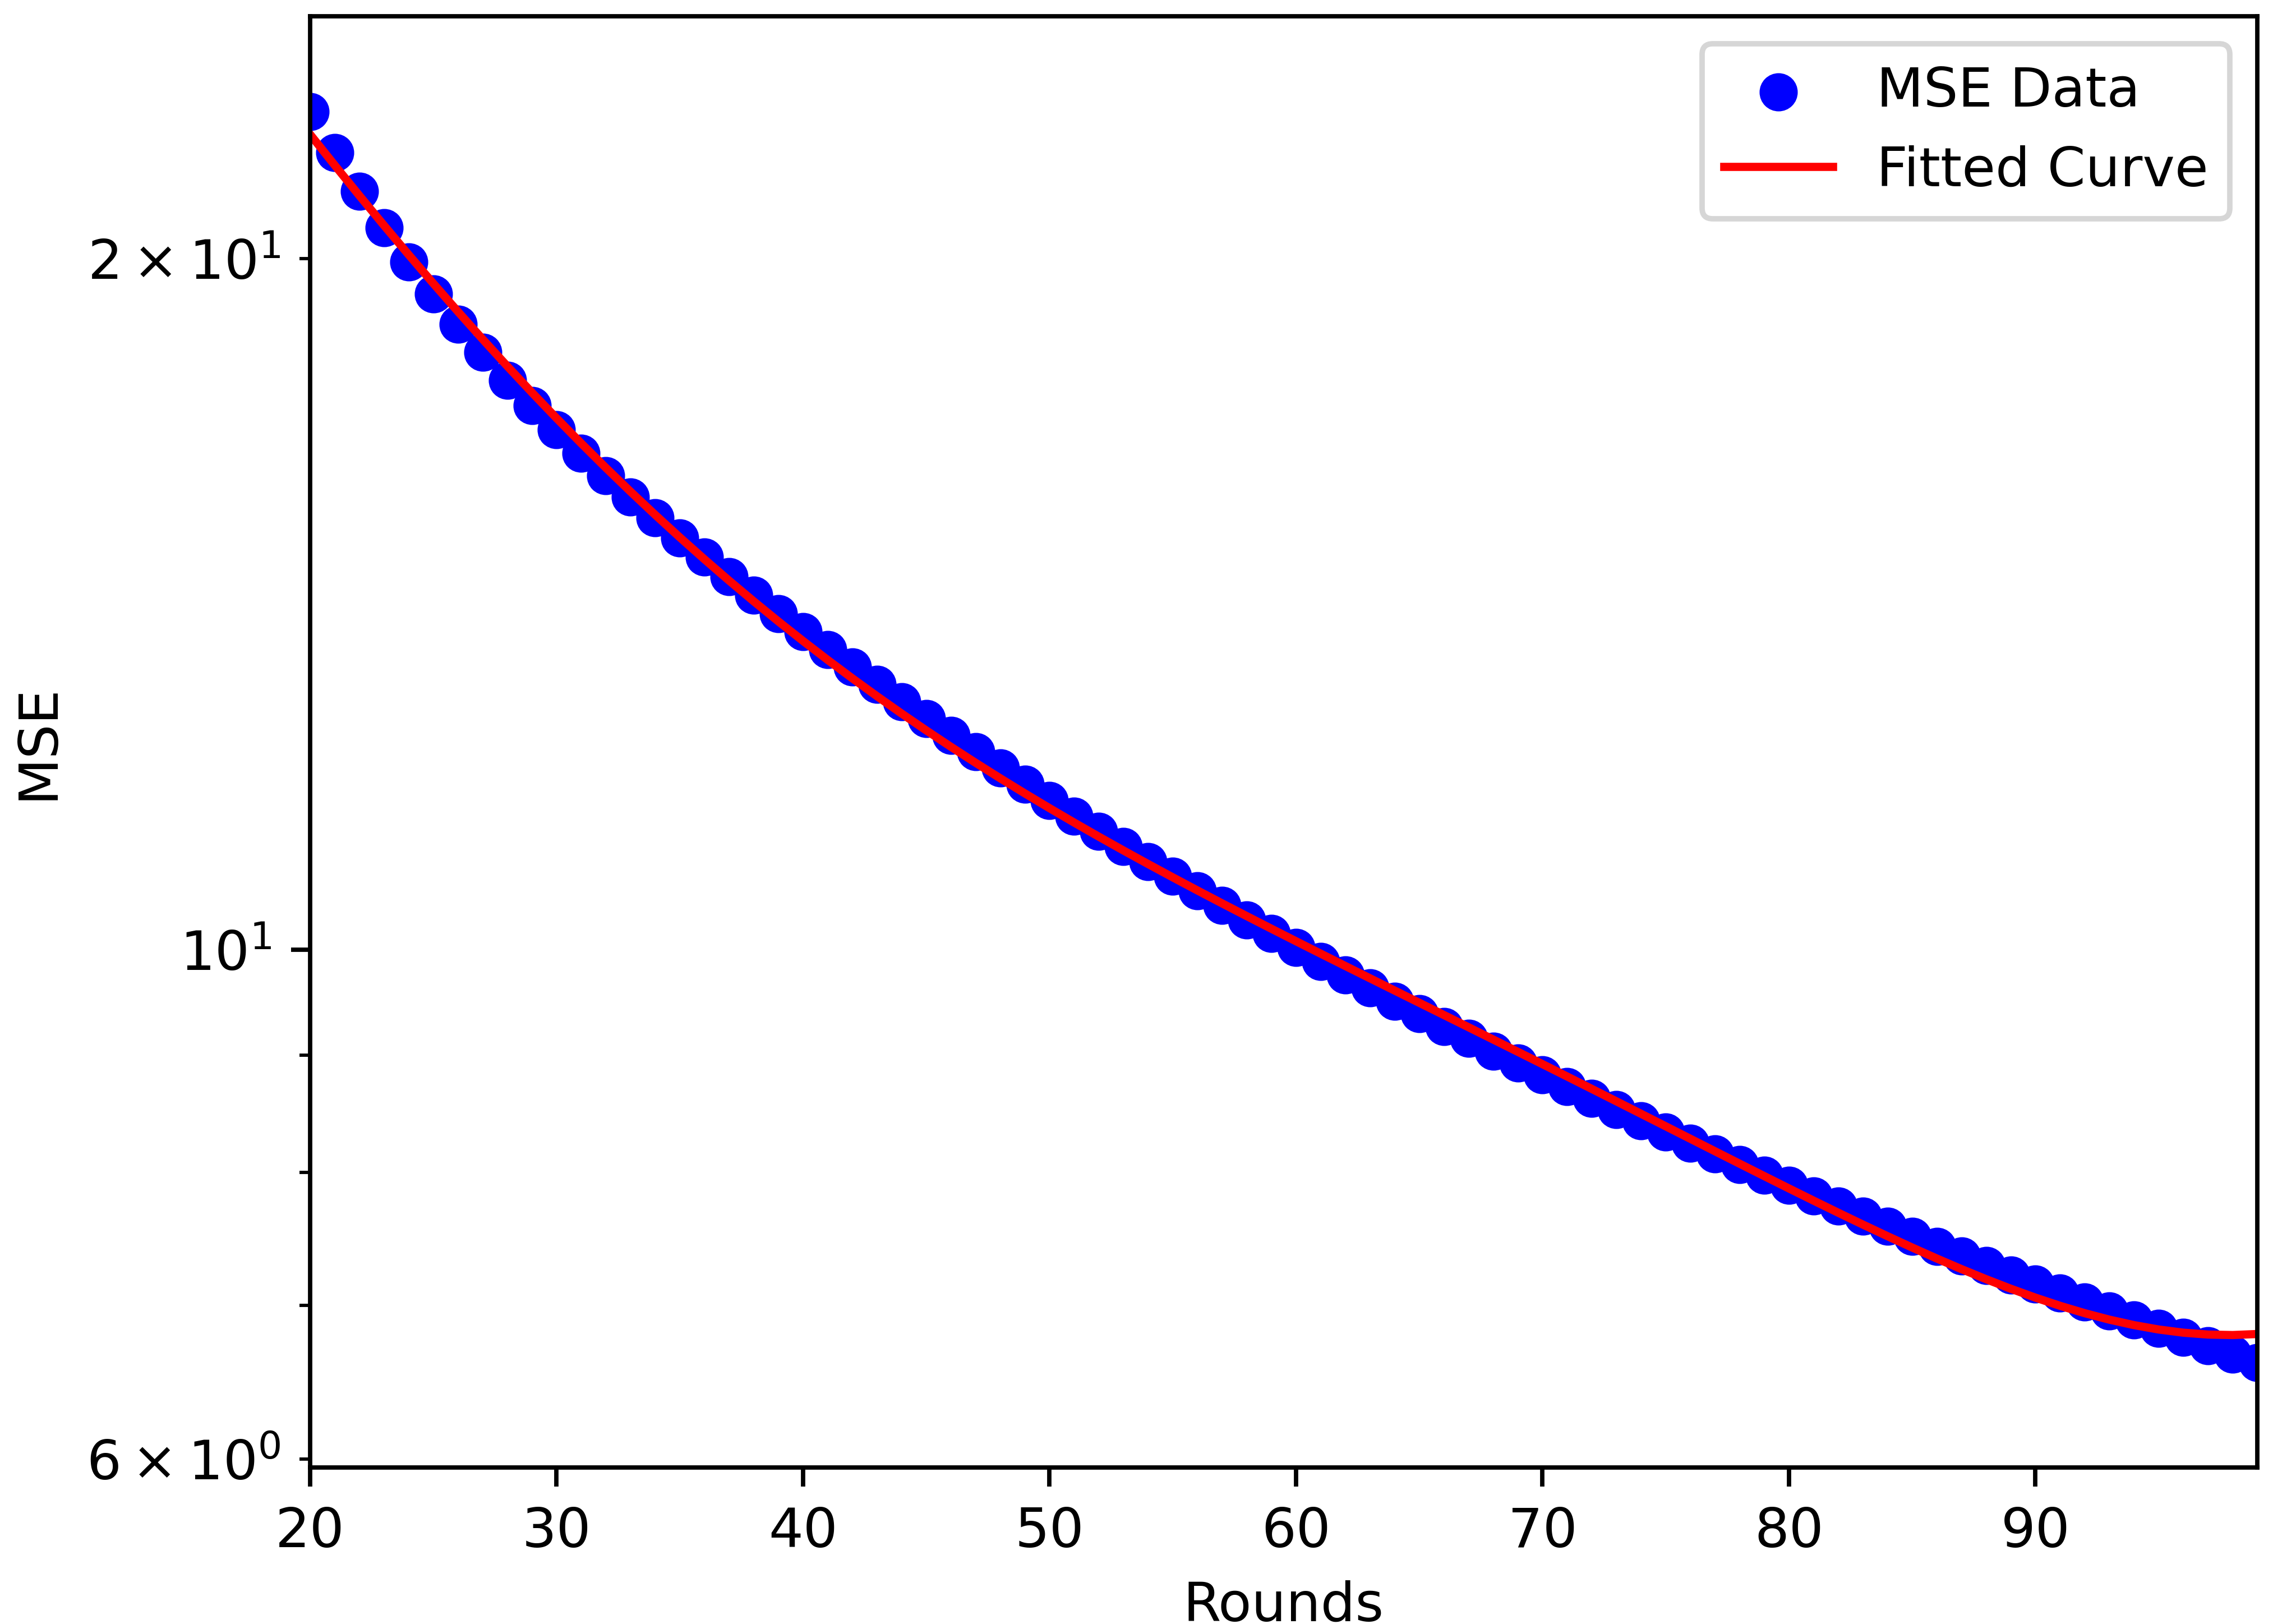
\includegraphics{figures/Simulation_outcomes/RingOfCliques/32x32/DAB/DAB_modelfitting_rounds_99_model_2.png}}
     \caption{$(32\times32)$-Ring of Cliques - polynomial regression fit - DAB}
     \label{fig:dabRingOfCliquesModelFit}
 \end{figure}
\begin{figure}[]
    \centering
    \scalebox{0.8}{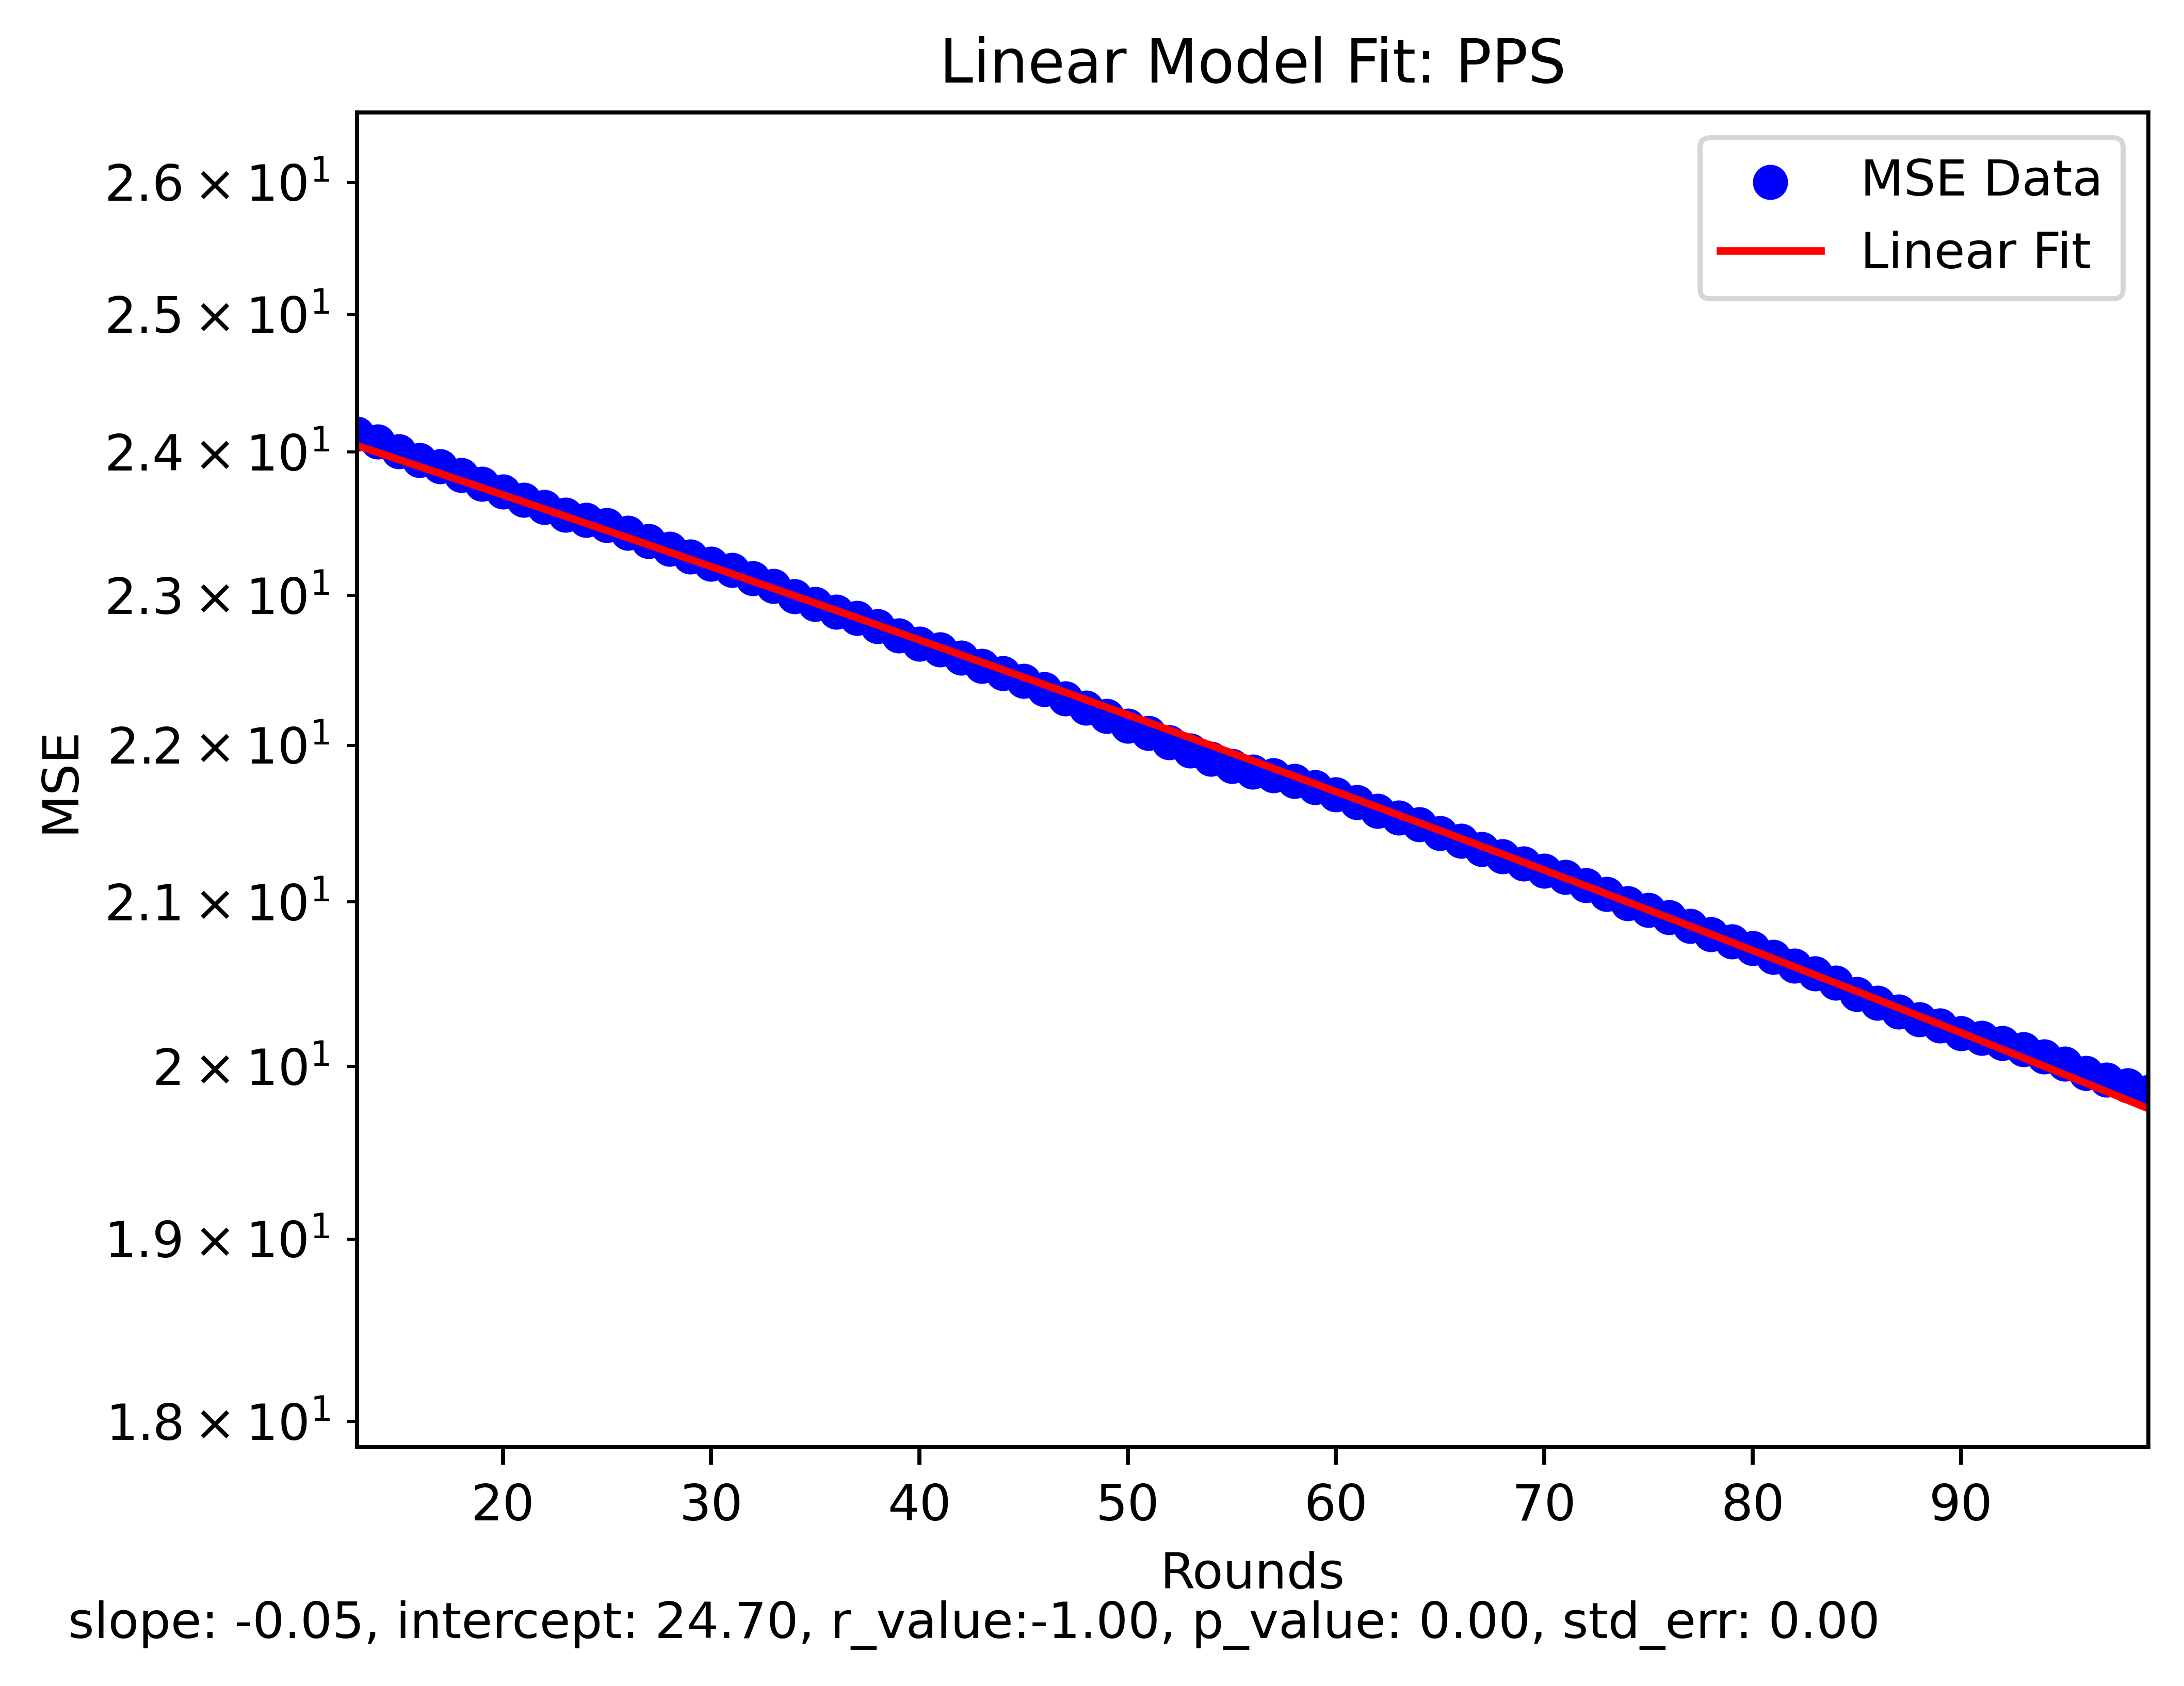
\includegraphics{figures/Simulation_outcomes/RingOfCliques/32x32/PPS/PPS_modelfitting_rounds_99_model_0.png}}
    \caption{$(32\times32)$-Ring of Cliques - linear regression fit - PPS}
    \label{fig:ppsRingOfCliquesModelFit}
\end{figure}

\begin{figure}[]
    \centering
    \scalebox{0.8}{\includegraphics{figures/Simulation_outcomes/RingOfCliques/32x32/ATPPS/ATPPS_modelfitting_rounds_99_model_3.png}}
    \caption{$(32\times32)$-Ring of Cliques - logarithmic regression fit - ATPPS}
    \label{fig:atppsRingOfCliquesModelFit}
\end{figure}

\begin{figure}[!ht]
    \centering
        \subfloat[]{\includegraphics[width=0.49\linewidth]{figures/Simulation_outcomes/RingOfCliques/32x32/DAB_vs_PPS_vs_ATPPS_slopesheatmap_100rounds_log_linear.png}}
    \hfil
        \subfloat[]{\includegraphics[width=0.49\linewidth]{figures/Simulation_outcomes/RingOfCliques/32x32/DAB_vs_PPS_vs_ATPPS_slopesheatmap_100rounds_log_log.png}}
    \caption{$(32\times32)$-Ring of Cliques - heat map of slopes per region - log-linear and log-log}
        \label{fig:ringOfCliquesslopes}
\end{figure}

In the following experiments, the structure of the Ring of Cliques is reorganized. The number of cliques is increased from $2^{5}$ to $2^{7}$ in subsection \ref{subsec:128_8ROC}, which results in a decrease in the size of each clique to $2^{3}$. Subsection \ref{subsec:8_128ROC} covers the experiment where the clique size is increased, while the number of cliques is decreased by the same magnitude.

\subsection{(128 x 8)-Ring of Cliques}\label{subsec:128_8ROC}
The clique size plays a crucial role for the efficacy of the DAB. The decreased clique size favors the DAB, which reduces the error in the network more rapidly than the Push-Pull Sum-based algorithms in the (128 x 8)-Ring of Cliques $ROC_{128,8}$, as seen in figure \ref{fig:128x8RingOfCliquesLog_LogLog}. All the load balancing algorithms show a rapid decrease of error in the network, indicated by the steep negative slopes as visualized in figure \ref{fig:128x8ringOfCliquesslopes} b). The Push-Pull Sum-based algorithms show an initial slope of -1.3, whereas the DAB achieves an even steeper slope of -1.4 in the start region (rounds 1 to 5). After this initial sharp decline, the error reduction slows down. However, DAB still maintains the steepest slope, with an average reduction of -0.95 per round, followed by ATPPS (-0.89) and PPS (-0.79). The curves in this region are relatively flat, as observed in the log-log representation in figure \ref{fig:128x8RingOfCliquesLog_LogLog} a). The decrease effect diminishes as the error of the network is already relatively low in the end region. At round 100, the final MSE values highlight the effectiveness of each algorithm. DAB achieves the lowest MSE of 10.64, ATPPS follows closely with 13.68. PPS results in the highest MSE of 22.33. Compared to $ROC_{32,32}$, the load balancing algorithms further reduced the error by 2 to 4 units. The ATPPS showed the most improvement, lowering the MSE by 5 units, followed by DAB (4 units) and PPS (2 units).

All three load balancing algorithms were fitted to fourth-degree polynomials. The best-fit equations are as follows: DAB's MSE data is fitted to a fourth-degree polynomial:
\begin{align}
    MSE_r=5.45\times 10 ^{-7}r^{4}-1.7\times 10^{-4}r^{3}+0.02r^{2}-1.33r+46.71    
\end{align}
(figure \ref{fig:128x8dabRingOfCliquesModelFit}), as are the PPS:
\begin{align}
    MSE_r=1.04\times 10 ^{-6}r^{4}-3.41\times 10^{-4}r^{3}+0.04r^{2}-2.73r+97.58    
\end{align}
(figure \ref{fig:128x8ppsRingOfCliquesModelFit}) and the ATPPS:
\begin{align}
    MSE_r=9.54\times 10^{-7}r^{4}-2.93\times 10^{-4}r^{3}+0.03r^{2}-2.05r+67.02    
\end{align}
(figure \ref{fig:128x8atppsRingOfCliquesModelFit}).

\begin{figure}[!ht]
    \centering
        \subfloat[]{\includegraphics[width=0.49\linewidth]{figures/Simulation_outcomes/RingOfCliques/128x8/DAB_vs_PPS_RoC_r100_n1024_averaged_log.png}}
    \hfil
        \subfloat[]{\includegraphics[width=0.49\linewidth]{figures/Simulation_outcomes/RingOfCliques/128x8/DAB_vs_PPS_RoC_r100_n1024_averaged_loglog.png}}
    \caption{$(128\times8)$-Ring of Cliques - mean squared error per rounds - log-linear and log-log}
        \label{fig:128x8RingOfCliquesLog_LogLog}
\end{figure}

\begin{figure}[]
     \centering
     \scalebox{0.8}{\includegraphics{figures/Simulation_outcomes/RingOfCliques/128x8/DAB/DAB_modelfitting_rounds_99_model_2.png}}
     \caption{$(128\times8)$-Ring of Cliques - polynomial regression fit - DAB}
     \label{fig:128x8dabRingOfCliquesModelFit}
\end{figure}
\begin{figure}[]
    \centering
    \scalebox{0.8}{\includegraphics{figures/Simulation_outcomes/RingOfCliques/128x8/PPS/PPS_modelfitting_rounds_99_model_2.png}}
    \caption{$(128\times8)$-Ring of Cliques - polynomial regression fit - PPS}
    \label{fig:128x8ppsRingOfCliquesModelFit}
\end{figure}

\begin{figure}[]
    \centering
    \scalebox{0.8}{\includegraphics{figures/Simulation_outcomes/RingOfCliques/128x8/ATPPS/ATPPS_modelfitting_rounds_99_model_2.png}}
    \caption{$(128\times8)$-Ring of Cliques - polynomial regression fit - ATPPS}
    \label{fig:128x8atppsRingOfCliquesModelFit}
\end{figure}

\begin{figure}[!ht]
    \centering
        \subfloat[]{\includegraphics[width=0.49\linewidth]{figures/Simulation_outcomes/RingOfCliques/128x8/DAB_vs_PPS_vs_ATPPS_slopesheatmap_100rounds_log_linear.png}}
    \hfil
        \subfloat[]{\includegraphics[width=0.49\linewidth]{figures/Simulation_outcomes/RingOfCliques/128x8/DAB_vs_PPS_vs_ATPPS_slopesheatmap_100rounds_log_log.png}}
    \caption{$(128\times8)$-Ring of Cliques - heat map of slopes per region - log-linear and log-log}
        \label{fig:128x8ringOfCliquesslopes}
\end{figure}

\subsection{(8 x 128)-Ring of Cliques}\label{subsec:8_128ROC}
Increasing the clique size and reducing the number of cliques favors the Push-Pull Sum-based algorithms (PPS and ATPPS), which exhibit a steep decrease in error during the first 5 rounds of the simulation in the (8 x 128)-Ring of Cliques $ROC_{8,128}$ (figure \ref{fig:8x128RingOfCliquesLog_LogLog}). PPS and ATPPS achieve an error reduction of approximately -2 on average for the start region. DAB shows a more moderate decrease of -0.12 in the same period. The error reduction slows, since the error of the network is already very low, showing an MSE in this region of around $-30$ for the Push-Pull Sum-based algorithms. In the middle region, the state of the network managed by the DAB is still very unbalanced, thus the balance potential is higher. The Push-Pull Sum-based algorithms reduce the error by around $-0.13$ for the ATPPS and $-0.01$ for the PPS in the final region, while the DAB shows a still very high value of approximately $-2.1$. The steep decrease and the low MSE values after rounds 5 and 10 stem from the fast error reduction in the cliques. Compared to the experiment in the $ROC_{8, 128}$ in \ref{subsec:128_8ROC}, the error after 100 rounds drops to lower values. The final MSE values for the DAB are 5.18 compared to 5.95 for the PPS and 4.56 for the ATPPS. In the final phase (rounds 12 to 100), the DAB slowly catches up to the Push-Pull Sum-based algorithms. However, both PPS and ATPPS achieve a well-balanced network state by round 10, by reducing the error to an MSE of 7. In the following rounds the inter-clique error reduction follows. The PPS algorithm struggles in this phase due to its randomized selection of transfer partners, which slows down further convergence. The ATPPS has an advantage compared to the PPS here since it prioritizes the bridging nodes once its neighbors within the clique are already balanced. This elaborates why the PPS curve is mostly stagnating, while the ATPPS curve shows a downward trend. The stagnating trend between rounds 20 to 100 is expressed by the linear mode fit in figure \ref{fig:8x128ppsRingOfCliquesModelFit}. The best-fit model follows the equation:
\begin{align}
    MSE_r=-1.5*10^{-3}r+6.05. 
\end{align}
The slope of $-1.5*10^{-3}$ is very small. The error in the network is barely reduced in this area. The behavior of the PPS is captured by this simple model. It does not involve any accelerations like in the exponential model. The PPS curve shows a more complex relation between the MSE reduction over the rounds, namely a polynomial of degree 2 following the equation:
\begin{align}
    MSE_r=6.07\times 10^{-5}r^{2}-0.02r+6.39    
\end{align}
(figure \ref{fig:8x128ppsRingOfCliquesModelFit}). The DAB does not follow a single power relationship in this region. Between rounds 15 and 50, the error reduction can be expressed by a third-degree polynomial:
\begin{align}
    MSE_r=-3.33\times 10^{-3}r^{3}+0.63r^{2}-40.23r+872.75    
\end{align}
(figure \ref{fig:8x128atppsRingOfCliquesModelFit} a)), while in later rounds the power relation is a bit more complex, expressed by a fourth-degree polynomial following the equation:
\begin{align}
    MSE_r=2.96 \times 10^{-6}r^{4}-9.97\times 10^{-3}r^{3}+0.13r^{2}-7.16r+161.73    
\end{align}
(figure \ref{fig:8x128atppsRingOfCliquesModelFit} b)).

Snippets of the simulation results confirm that within each clique, loads are balanced. However, inter-clique load balancing remains pending, which indicates that global equilibrium is not fully achieved. Listing \ref{lst:exampleROCOutcomes} shows the simulation outcomes of two connected cliques balanced by the ATPPS in round 100. While the first clique converged to a value of around $46.35$, the second clique averaged to approximately $47.90$. The ground truth of the first clique is $45.89$, and the ground truth of the second clique is $48.13$. So the simulation outcomes and the ground truths align; however, the averages do not align with the ground truth of the Ring of Cliques (which is $49.09$) itself. The PPS simulation outcomes show a similar behavior.
\begin{figure}[!ht]
    \centering
        \subfloat[]{\includegraphics[width=0.49\linewidth]{figures/Simulation_outcomes/RingOfCliques/8x128/DAB_vs_PPS_RoC_r100_n1024_averaged_log.png}}
    \hfil
        \subfloat[]{\includegraphics[width=0.49\linewidth]{figures/Simulation_outcomes/RingOfCliques/8x128/DAB_vs_PPS_RoC_r100_n1024_averaged_loglog.png}}
    \caption{$(8\times128)$-Ring of Cliques - mean squared error per rounds - log-linear and log-log}
        \label{fig:8x128RingOfCliquesLog_LogLog}
\end{figure}

\begin{figure}[!ht]
    \centering
        \subfloat[]{\includegraphics[width=0.49\linewidth]{figures/Simulation_outcomes/RingOfCliques/8x128/DAB/DAB_modelfitting_rounds_49_model_2.png}}
    \hfil
        \subfloat[]{\includegraphics[width=0.49\linewidth]{figures/Simulation_outcomes/RingOfCliques/8x128/DAB/DAB_modelfitting_rounds_99_model_2.png}}
    \caption{$(8\times128)$-Ring of Cliques - polynomial regression fit - DAB; rounds 20-50 and 55-100}
        \label{fig:8x128dabRingOfCliquesModelFit}
\end{figure}
\begin{figure}[]
    \centering
    \scalebox{0.8}{\includegraphics{figures/Simulation_outcomes/RingOfCliques/8x128/PPS/PPS_modelfitting_rounds_99_model_0.png}}
    \caption{$(8\times128)$-Ring of Cliques - linear regression fit - PPS}
    \label{fig:8x128ppsRingOfCliquesModelFit}
\end{figure}

\begin{figure}[]
    \centering
    \scalebox{0.8}{\includegraphics{figures/Simulation_outcomes/RingOfCliques/8x128/ATPPS/ATPPS_modelfitting_rounds_99_model_2.png}}
    \caption{$(8\times128)$-Ring of Cliques - polynomial regression fit - ATPPS}
    \label{fig:8x128atppsRingOfCliquesModelFit}
\end{figure}

\begin{figure}[!ht]
    \centering
        \subfloat[]{\includegraphics[width=0.49\linewidth]{figures/Simulation_outcomes/RingOfCliques/8x128/DAB_vs_PPS_vs_ATPPS_slopesheatmap_100rounds_log_linear.png}}
    \hfil
        \subfloat[]{\includegraphics[width=0.49\linewidth]{figures/Simulation_outcomes/RingOfCliques/8x128/DAB_vs_PPS_vs_ATPPS_slopesheatmap_100rounds_log_log.png}}
    \caption{$(8\times128)$-Ring of Cliques - heat map of slopes per region - log-linear and log-log}
        \label{fig:8x128ringOfCliquesslopes}
\end{figure}

\begin{lstlisting}[caption=Snippet of simulation outcomes - ATPPS: Experiment 2, captionpos=b, label=lst:exampleROCOutcomes]
# start: first clique
ID 0	 sum 23.703116631927735	 weight 0.5112902995975737	 Average 46.359410007551446
ID 1	 sum 39.52476483621201	 weight 0.852801600538612	 Average 46.34696371494727
ID 2	 sum 8.793798989811481	 weight 0.18958634077240344	 Average 46.38413798158778
...
ID 125	 sum 94.3005473042508	 weight 2.0354736681273184	 Average 46.32855181615266
ID 126	 sum 145.10578299145917	 weight 3.1321941681390815	 Average 46.32719914604474
ID 127	 sum 149.43516229432458	 weight 3.222997634840688	 Average 46.365272092950555
# end: first clique

# start: second clique
ID 128	 sum 198.97437468622982	 weight 4.149869252421544	 Average 47.947143050380134
ID 129	 sum 168.24642313171216	 weight 3.5107838866374186	 Average 47.92275131832632
ID 130	 sum 35.6266112221637	 weight 0.7449330697151406	 Average 47.82525124812511
...
ID 253	 sum 63.87360335784297	 weight 1.3317373880292274	 Average 47.962611797185005
ID 254	 sum 15.173810743452982	 weight 0.31637895519911763	 Average 47.96087253623784
ID 255	 sum 19.982619800226413	 weight 0.4175626540105257	 Average 47.85538076334456
# end: second clique
\end{lstlisting}